% Options for packages loaded elsewhere
\PassOptionsToPackage{unicode}{hyperref}
\PassOptionsToPackage{hyphens}{url}
%
\documentclass[
]{book}
\usepackage{lmodern}
\usepackage{amsmath}
\usepackage{ifxetex,ifluatex}
\ifnum 0\ifxetex 1\fi\ifluatex 1\fi=0 % if pdftex
  \usepackage[T1]{fontenc}
  \usepackage[utf8]{inputenc}
  \usepackage{textcomp} % provide euro and other symbols
  \usepackage{amssymb}
\else % if luatex or xetex
  \usepackage{unicode-math}
  \defaultfontfeatures{Scale=MatchLowercase}
  \defaultfontfeatures[\rmfamily]{Ligatures=TeX,Scale=1}
\fi
% Use upquote if available, for straight quotes in verbatim environments
\IfFileExists{upquote.sty}{\usepackage{upquote}}{}
\IfFileExists{microtype.sty}{% use microtype if available
  \usepackage[]{microtype}
  \UseMicrotypeSet[protrusion]{basicmath} % disable protrusion for tt fonts
}{}
\makeatletter
\@ifundefined{KOMAClassName}{% if non-KOMA class
  \IfFileExists{parskip.sty}{%
    \usepackage{parskip}
  }{% else
    \setlength{\parindent}{0pt}
    \setlength{\parskip}{6pt plus 2pt minus 1pt}}
}{% if KOMA class
  \KOMAoptions{parskip=half}}
\makeatother
\usepackage{xcolor}
\IfFileExists{xurl.sty}{\usepackage{xurl}}{} % add URL line breaks if available
\IfFileExists{bookmark.sty}{\usepackage{bookmark}}{\usepackage{hyperref}}
\hypersetup{
  pdftitle={Bayesian Computation with R Scripts},
  pdfauthor={Jim Albert},
  hidelinks,
  pdfcreator={LaTeX via pandoc}}
\urlstyle{same} % disable monospaced font for URLs
\usepackage{color}
\usepackage{fancyvrb}
\newcommand{\VerbBar}{|}
\newcommand{\VERB}{\Verb[commandchars=\\\{\}]}
\DefineVerbatimEnvironment{Highlighting}{Verbatim}{commandchars=\\\{\}}
% Add ',fontsize=\small' for more characters per line
\usepackage{framed}
\definecolor{shadecolor}{RGB}{248,248,248}
\newenvironment{Shaded}{\begin{snugshade}}{\end{snugshade}}
\newcommand{\AlertTok}[1]{\textcolor[rgb]{0.94,0.16,0.16}{#1}}
\newcommand{\AnnotationTok}[1]{\textcolor[rgb]{0.56,0.35,0.01}{\textbf{\textit{#1}}}}
\newcommand{\AttributeTok}[1]{\textcolor[rgb]{0.77,0.63,0.00}{#1}}
\newcommand{\BaseNTok}[1]{\textcolor[rgb]{0.00,0.00,0.81}{#1}}
\newcommand{\BuiltInTok}[1]{#1}
\newcommand{\CharTok}[1]{\textcolor[rgb]{0.31,0.60,0.02}{#1}}
\newcommand{\CommentTok}[1]{\textcolor[rgb]{0.56,0.35,0.01}{\textit{#1}}}
\newcommand{\CommentVarTok}[1]{\textcolor[rgb]{0.56,0.35,0.01}{\textbf{\textit{#1}}}}
\newcommand{\ConstantTok}[1]{\textcolor[rgb]{0.00,0.00,0.00}{#1}}
\newcommand{\ControlFlowTok}[1]{\textcolor[rgb]{0.13,0.29,0.53}{\textbf{#1}}}
\newcommand{\DataTypeTok}[1]{\textcolor[rgb]{0.13,0.29,0.53}{#1}}
\newcommand{\DecValTok}[1]{\textcolor[rgb]{0.00,0.00,0.81}{#1}}
\newcommand{\DocumentationTok}[1]{\textcolor[rgb]{0.56,0.35,0.01}{\textbf{\textit{#1}}}}
\newcommand{\ErrorTok}[1]{\textcolor[rgb]{0.64,0.00,0.00}{\textbf{#1}}}
\newcommand{\ExtensionTok}[1]{#1}
\newcommand{\FloatTok}[1]{\textcolor[rgb]{0.00,0.00,0.81}{#1}}
\newcommand{\FunctionTok}[1]{\textcolor[rgb]{0.00,0.00,0.00}{#1}}
\newcommand{\ImportTok}[1]{#1}
\newcommand{\InformationTok}[1]{\textcolor[rgb]{0.56,0.35,0.01}{\textbf{\textit{#1}}}}
\newcommand{\KeywordTok}[1]{\textcolor[rgb]{0.13,0.29,0.53}{\textbf{#1}}}
\newcommand{\NormalTok}[1]{#1}
\newcommand{\OperatorTok}[1]{\textcolor[rgb]{0.81,0.36,0.00}{\textbf{#1}}}
\newcommand{\OtherTok}[1]{\textcolor[rgb]{0.56,0.35,0.01}{#1}}
\newcommand{\PreprocessorTok}[1]{\textcolor[rgb]{0.56,0.35,0.01}{\textit{#1}}}
\newcommand{\RegionMarkerTok}[1]{#1}
\newcommand{\SpecialCharTok}[1]{\textcolor[rgb]{0.00,0.00,0.00}{#1}}
\newcommand{\SpecialStringTok}[1]{\textcolor[rgb]{0.31,0.60,0.02}{#1}}
\newcommand{\StringTok}[1]{\textcolor[rgb]{0.31,0.60,0.02}{#1}}
\newcommand{\VariableTok}[1]{\textcolor[rgb]{0.00,0.00,0.00}{#1}}
\newcommand{\VerbatimStringTok}[1]{\textcolor[rgb]{0.31,0.60,0.02}{#1}}
\newcommand{\WarningTok}[1]{\textcolor[rgb]{0.56,0.35,0.01}{\textbf{\textit{#1}}}}
\usepackage{longtable,booktabs}
\usepackage{calc} % for calculating minipage widths
% Correct order of tables after \paragraph or \subparagraph
\usepackage{etoolbox}
\makeatletter
\patchcmd\longtable{\par}{\if@noskipsec\mbox{}\fi\par}{}{}
\makeatother
% Allow footnotes in longtable head/foot
\IfFileExists{footnotehyper.sty}{\usepackage{footnotehyper}}{\usepackage{footnote}}
\makesavenoteenv{longtable}
\usepackage{graphicx}
\makeatletter
\def\maxwidth{\ifdim\Gin@nat@width>\linewidth\linewidth\else\Gin@nat@width\fi}
\def\maxheight{\ifdim\Gin@nat@height>\textheight\textheight\else\Gin@nat@height\fi}
\makeatother
% Scale images if necessary, so that they will not overflow the page
% margins by default, and it is still possible to overwrite the defaults
% using explicit options in \includegraphics[width, height, ...]{}
\setkeys{Gin}{width=\maxwidth,height=\maxheight,keepaspectratio}
% Set default figure placement to htbp
\makeatletter
\def\fps@figure{htbp}
\makeatother
\setlength{\emergencystretch}{3em} % prevent overfull lines
\providecommand{\tightlist}{%
  \setlength{\itemsep}{0pt}\setlength{\parskip}{0pt}}
\setcounter{secnumdepth}{5}
\usepackage{booktabs}
\usepackage{amsthm}
\makeatletter
\def\thm@space@setup{%
  \thm@preskip=8pt plus 2pt minus 4pt
  \thm@postskip=\thm@preskip
}
\makeatother
\ifluatex
  \usepackage{selnolig}  % disable illegal ligatures
\fi
\usepackage[]{natbib}
\bibliographystyle{apalike}

\title{Bayesian Computation with R Scripts}
\author{Jim Albert}
\date{2020-12-18}

\begin{document}
\maketitle

{
\setcounter{tocdepth}{1}
\tableofcontents
}
\hypertarget{preface}{%
\chapter{Preface}\label{preface}}

This book contains all of the R scripts and associated output for Chapters 2 through 10 of \emph{Bayesian Computation with R} second edition.

In these scripts, I have avoided the use of the \texttt{attach()} function and spaces have been added to increase readability.

\hypertarget{introduction-to-bayesian-thinking}{%
\chapter{Introduction to Bayesian Thinking}\label{introduction-to-bayesian-thinking}}

\hypertarget{learning-about-the-proportion-of-heavy-sleepers}{%
\section{Learning About the Proportion of Heavy Sleepers}\label{learning-about-the-proportion-of-heavy-sleepers}}

Want to learn about \(p\), the proportion of heavy sleepers. Take a sample of 27 students and 11 are heavy sleepers.

\hypertarget{using-a-discrete-prior}{%
\section{Using a Discrete Prior}\label{using-a-discrete-prior}}

\begin{Shaded}
\begin{Highlighting}[]
\FunctionTok{library}\NormalTok{(LearnBayes)}
\end{Highlighting}
\end{Shaded}

The prior for \(p\):

\begin{Shaded}
\begin{Highlighting}[]
\NormalTok{p }\OtherTok{\textless{}{-}} \FunctionTok{seq}\NormalTok{(}\FloatTok{0.05}\NormalTok{, }\FloatTok{0.95}\NormalTok{, }\AttributeTok{by =} \FloatTok{0.1}\NormalTok{)}
\NormalTok{prior }\OtherTok{\textless{}{-}} \FunctionTok{c}\NormalTok{(}\DecValTok{1}\NormalTok{, }\FloatTok{5.2}\NormalTok{, }\DecValTok{8}\NormalTok{, }\FloatTok{7.2}\NormalTok{, }\FloatTok{4.6}\NormalTok{, }\FloatTok{2.1}\NormalTok{, }
           \FloatTok{0.7}\NormalTok{, }\FloatTok{0.1}\NormalTok{, }\DecValTok{0}\NormalTok{, }\DecValTok{0}\NormalTok{)}
\NormalTok{prior }\OtherTok{\textless{}{-}}\NormalTok{ prior }\SpecialCharTok{/} \FunctionTok{sum}\NormalTok{(prior)}
\FunctionTok{plot}\NormalTok{(p, prior, }\AttributeTok{type =} \StringTok{"h"}\NormalTok{, }
     \AttributeTok{ylab=}\StringTok{"Prior Probability"}\NormalTok{)}
\end{Highlighting}
\end{Shaded}

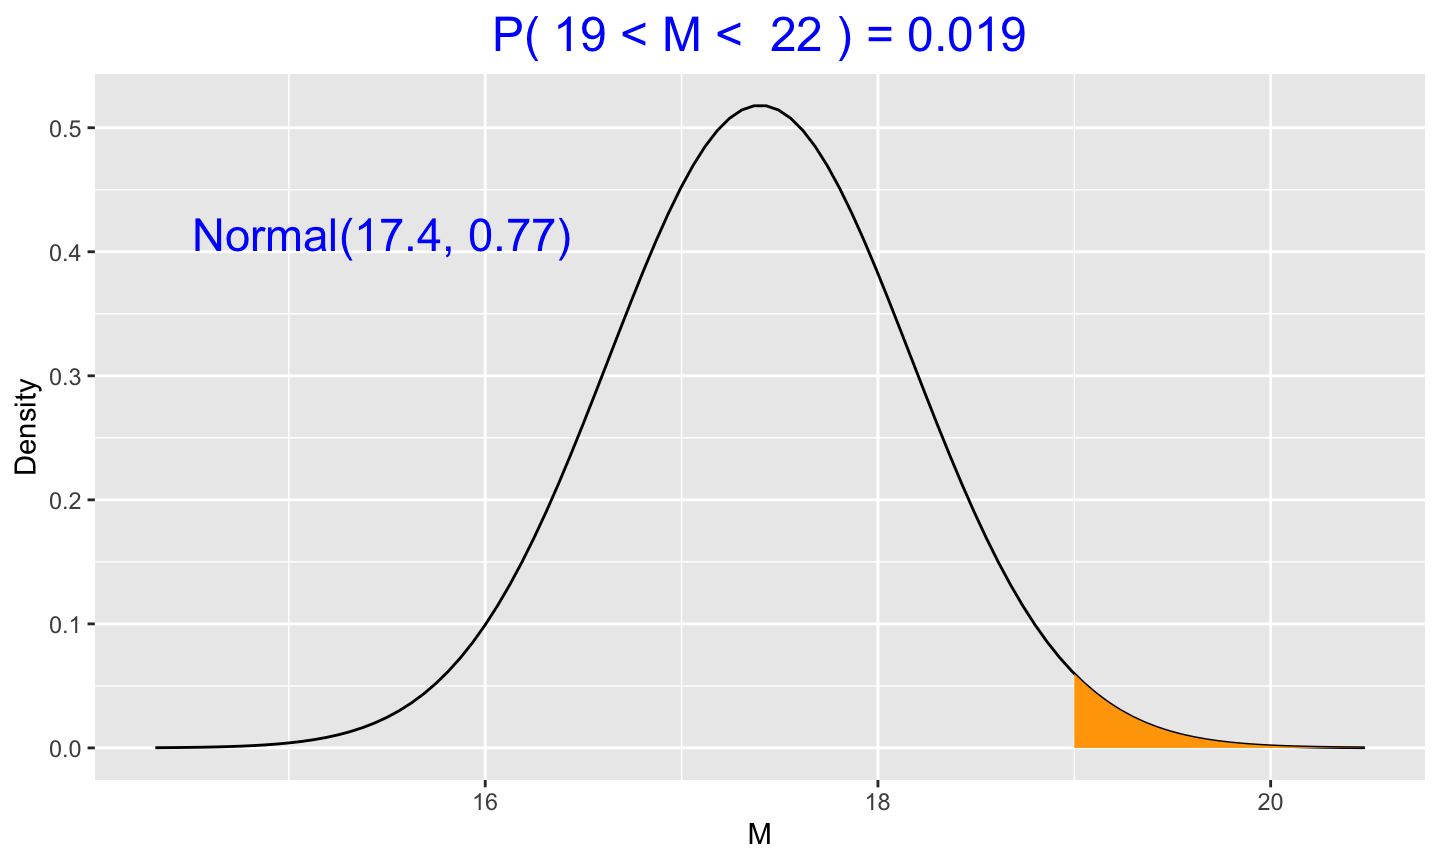
\includegraphics{bookdown-demo_files/figure-latex/unnamed-chunk-2-1.pdf}

The posterior for \(p\):

\begin{Shaded}
\begin{Highlighting}[]
\NormalTok{data }\OtherTok{\textless{}{-}} \FunctionTok{c}\NormalTok{(}\DecValTok{11}\NormalTok{, }\DecValTok{16}\NormalTok{)}
\NormalTok{post }\OtherTok{\textless{}{-}} \FunctionTok{pdisc}\NormalTok{(p, prior, data)}
\FunctionTok{round}\NormalTok{(}\FunctionTok{cbind}\NormalTok{(p, prior, post),}\DecValTok{2}\NormalTok{)}
\end{Highlighting}
\end{Shaded}

\begin{verbatim}
##          p prior post
##  [1,] 0.05  0.03 0.00
##  [2,] 0.15  0.18 0.00
##  [3,] 0.25  0.28 0.13
##  [4,] 0.35  0.25 0.48
##  [5,] 0.45  0.16 0.33
##  [6,] 0.55  0.07 0.06
##  [7,] 0.65  0.02 0.00
##  [8,] 0.75  0.00 0.00
##  [9,] 0.85  0.00 0.00
## [10,] 0.95  0.00 0.00
\end{verbatim}

\begin{Shaded}
\begin{Highlighting}[]
\FunctionTok{library}\NormalTok{(lattice)}
\NormalTok{PRIOR }\OtherTok{\textless{}{-}} \FunctionTok{data.frame}\NormalTok{(}\StringTok{"prior"}\NormalTok{, p, prior)}
\NormalTok{POST }\OtherTok{\textless{}{-}} \FunctionTok{data.frame}\NormalTok{(}\StringTok{"posterior"}\NormalTok{, p, post)}
\FunctionTok{names}\NormalTok{(PRIOR) }\OtherTok{\textless{}{-}} \FunctionTok{c}\NormalTok{(}\StringTok{"Type"}\NormalTok{, }\StringTok{"P"}\NormalTok{, }\StringTok{"Probability"}\NormalTok{)}
\FunctionTok{names}\NormalTok{(POST) }\OtherTok{\textless{}{-}} \FunctionTok{c}\NormalTok{(}\StringTok{"Type"}\NormalTok{,}\StringTok{"P"}\NormalTok{,}\StringTok{"Probability"}\NormalTok{)}
\NormalTok{data }\OtherTok{\textless{}{-}} \FunctionTok{rbind}\NormalTok{(PRIOR, POST)}
\end{Highlighting}
\end{Shaded}

\begin{Shaded}
\begin{Highlighting}[]
\FunctionTok{xyplot}\NormalTok{(Probability }\SpecialCharTok{\textasciitilde{}}\NormalTok{ P }\SpecialCharTok{|}\NormalTok{ Type, }\AttributeTok{data=}\NormalTok{data, }
       \AttributeTok{layout=}\FunctionTok{c}\NormalTok{(}\DecValTok{1}\NormalTok{,}\DecValTok{2}\NormalTok{), }\AttributeTok{type=}\StringTok{"h"}\NormalTok{, }\AttributeTok{lwd=}\DecValTok{3}\NormalTok{, }\AttributeTok{col=}\StringTok{"black"}\NormalTok{)}
\end{Highlighting}
\end{Shaded}

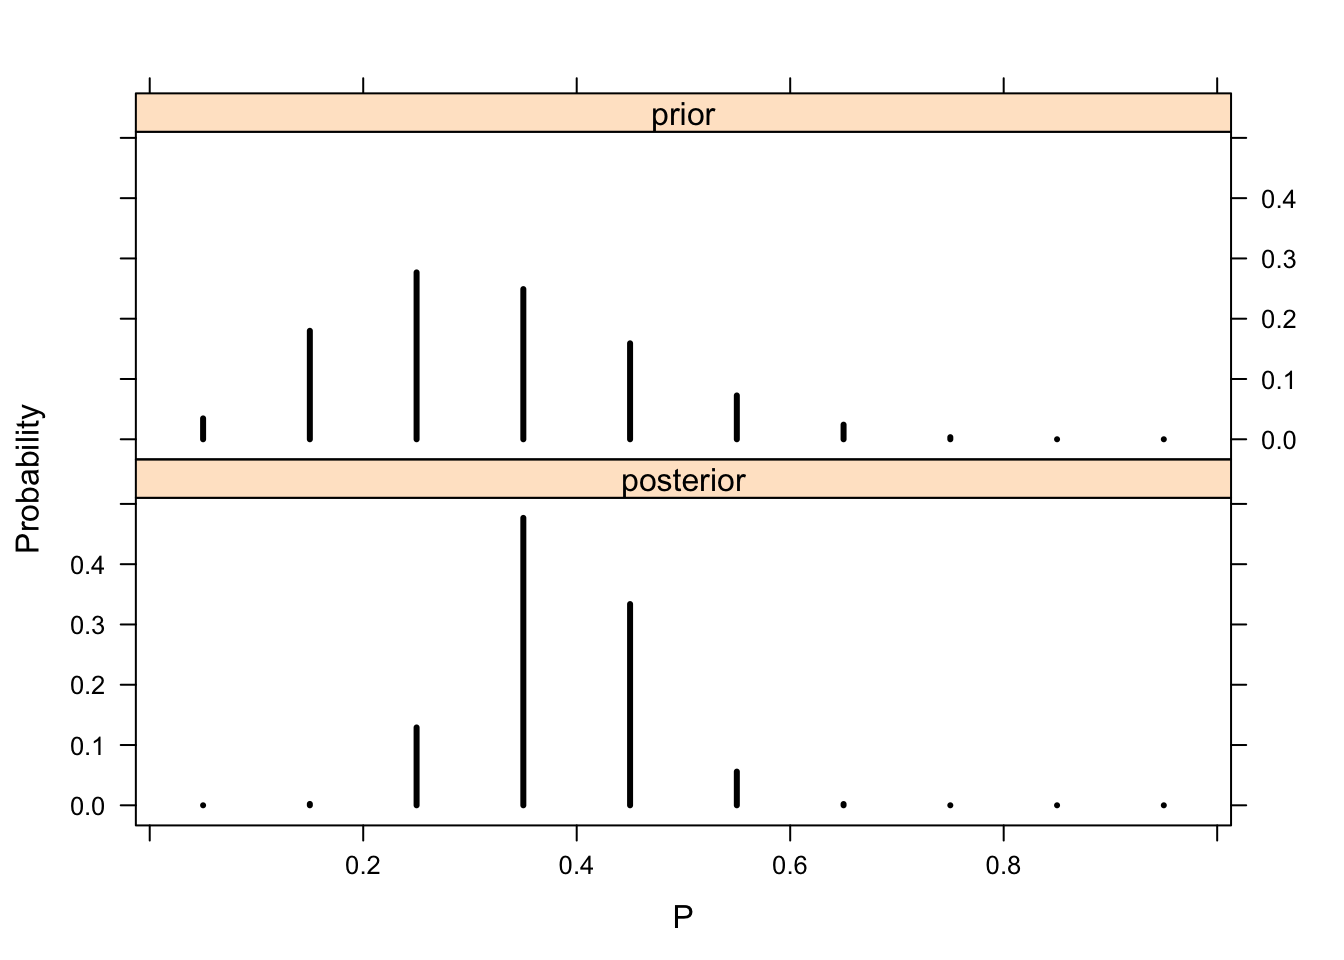
\includegraphics{bookdown-demo_files/figure-latex/unnamed-chunk-4-1.pdf}

\hypertarget{using-a-beta-prior}{%
\section{Using a Beta Prior}\label{using-a-beta-prior}}

Construct a beta prior for \(p\) by inputting two percentiles:

\begin{Shaded}
\begin{Highlighting}[]
\NormalTok{quantile2 }\OtherTok{\textless{}{-}} \FunctionTok{list}\NormalTok{(}\AttributeTok{p=}\NormalTok{.}\DecValTok{9}\NormalTok{, }\AttributeTok{x=}\NormalTok{.}\DecValTok{5}\NormalTok{)}
\NormalTok{quantile1 }\OtherTok{\textless{}{-}} \FunctionTok{list}\NormalTok{(}\AttributeTok{p=}\NormalTok{.}\DecValTok{5}\NormalTok{, }\AttributeTok{x=}\NormalTok{.}\DecValTok{3}\NormalTok{)}
\NormalTok{(ab }\OtherTok{\textless{}{-}} \FunctionTok{beta.select}\NormalTok{(quantile1,quantile2))}
\end{Highlighting}
\end{Shaded}

\begin{verbatim}
## [1] 3.26 7.19
\end{verbatim}

Bayesian triplot:

\begin{Shaded}
\begin{Highlighting}[]
\NormalTok{a }\OtherTok{\textless{}{-}}\NormalTok{ ab[}\DecValTok{1}\NormalTok{]}
\NormalTok{b }\OtherTok{\textless{}{-}}\NormalTok{ ab[}\DecValTok{2}\NormalTok{]}
\NormalTok{s }\OtherTok{\textless{}{-}} \DecValTok{11}
\NormalTok{f }\OtherTok{\textless{}{-}} \DecValTok{16}
\FunctionTok{curve}\NormalTok{(}\FunctionTok{dbeta}\NormalTok{(x, a }\SpecialCharTok{+}\NormalTok{ s, b }\SpecialCharTok{+}\NormalTok{ f), }\AttributeTok{from=}\DecValTok{0}\NormalTok{, }\AttributeTok{to=}\DecValTok{1}\NormalTok{, }
       \AttributeTok{xlab=}\StringTok{"p"}\NormalTok{, }\AttributeTok{ylab=}\StringTok{"Density"}\NormalTok{, }\AttributeTok{lty=}\DecValTok{1}\NormalTok{, }\AttributeTok{lwd=}\DecValTok{4}\NormalTok{)}
\FunctionTok{curve}\NormalTok{(}\FunctionTok{dbeta}\NormalTok{(x, s }\SpecialCharTok{+} \DecValTok{1}\NormalTok{, f }\SpecialCharTok{+} \DecValTok{1}\NormalTok{), }\AttributeTok{add=}\ConstantTok{TRUE}\NormalTok{, }
       \AttributeTok{lty=}\DecValTok{2}\NormalTok{, }\AttributeTok{lwd=}\DecValTok{4}\NormalTok{)}
\FunctionTok{curve}\NormalTok{(}\FunctionTok{dbeta}\NormalTok{(x, a, b), }\AttributeTok{add=}\ConstantTok{TRUE}\NormalTok{, }\AttributeTok{lty=}\DecValTok{3}\NormalTok{, }\AttributeTok{lwd=}\DecValTok{4}\NormalTok{)}
\FunctionTok{legend}\NormalTok{(.}\DecValTok{7}\NormalTok{, }\DecValTok{4}\NormalTok{, }\FunctionTok{c}\NormalTok{(}\StringTok{"Prior"}\NormalTok{, }\StringTok{"Likelihood"}\NormalTok{,}
                \StringTok{"Posterior"}\NormalTok{),}
       \AttributeTok{lty=}\FunctionTok{c}\NormalTok{(}\DecValTok{3}\NormalTok{, }\DecValTok{2}\NormalTok{, }\DecValTok{1}\NormalTok{), }\AttributeTok{lwd=}\FunctionTok{c}\NormalTok{(}\DecValTok{3}\NormalTok{, }\DecValTok{3}\NormalTok{, }\DecValTok{3}\NormalTok{))}
\end{Highlighting}
\end{Shaded}

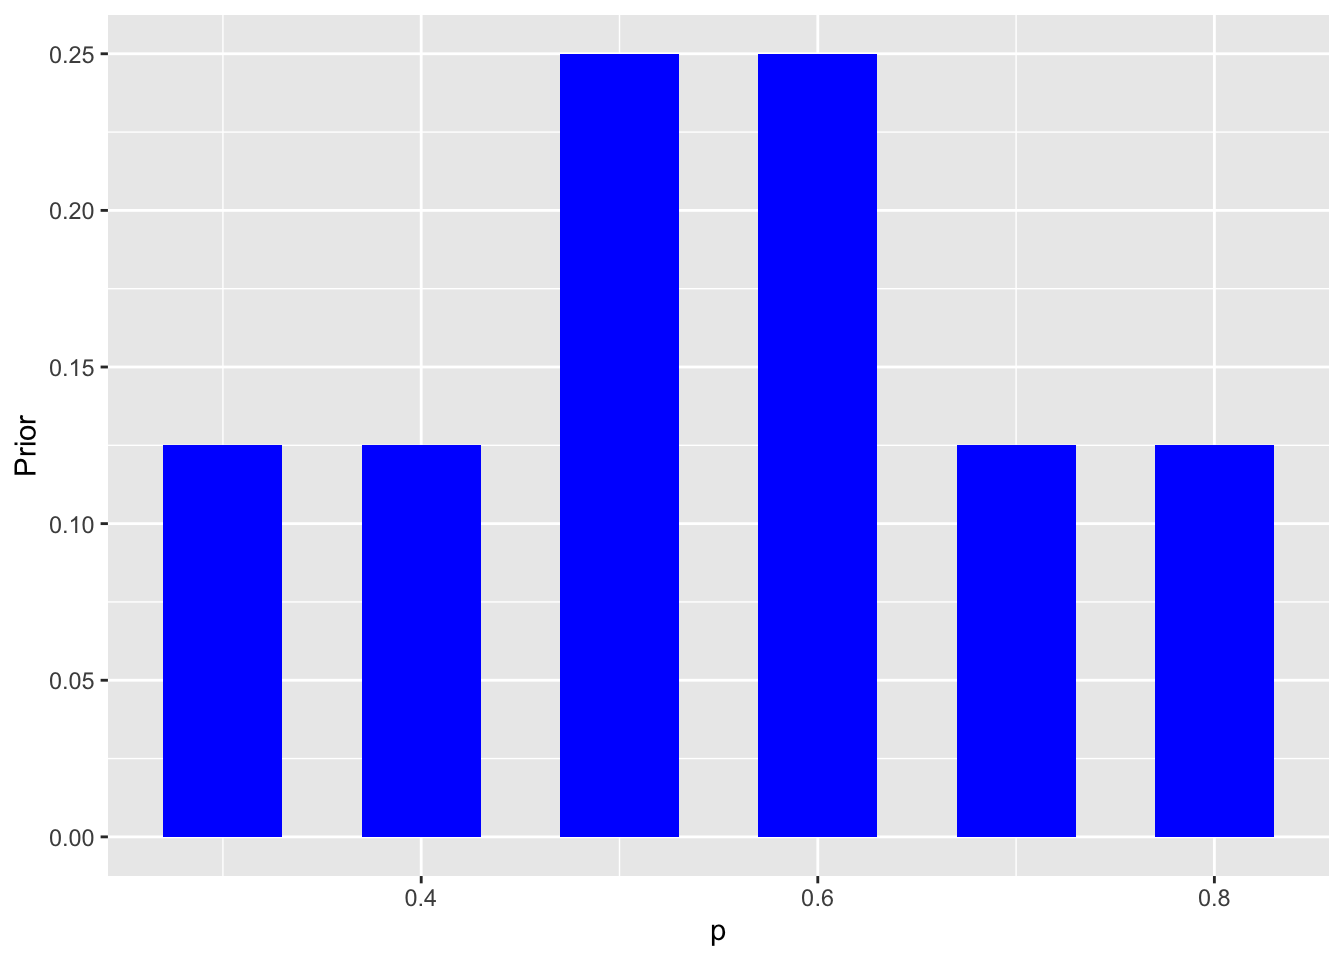
\includegraphics{bookdown-demo_files/figure-latex/unnamed-chunk-6-1.pdf}

Posterior summaries:

\begin{Shaded}
\begin{Highlighting}[]
\DecValTok{1} \SpecialCharTok{{-}} \FunctionTok{pbeta}\NormalTok{(}\FloatTok{0.5}\NormalTok{, a }\SpecialCharTok{+}\NormalTok{ s, b }\SpecialCharTok{+}\NormalTok{ f)}
\end{Highlighting}
\end{Shaded}

\begin{verbatim}
## [1] 0.0690226
\end{verbatim}

\begin{Shaded}
\begin{Highlighting}[]
\FunctionTok{qbeta}\NormalTok{(}\FunctionTok{c}\NormalTok{(}\FloatTok{0.05}\NormalTok{, }\FloatTok{0.95}\NormalTok{), a }\SpecialCharTok{+}\NormalTok{ s, b }\SpecialCharTok{+}\NormalTok{ f)}
\end{Highlighting}
\end{Shaded}

\begin{verbatim}
## [1] 0.2555267 0.5133608
\end{verbatim}

Simulating from posterior:

\begin{Shaded}
\begin{Highlighting}[]
\NormalTok{ps }\OtherTok{\textless{}{-}} \FunctionTok{rbeta}\NormalTok{(}\DecValTok{1000}\NormalTok{, a }\SpecialCharTok{+}\NormalTok{ s, b }\SpecialCharTok{+}\NormalTok{ f)}
\end{Highlighting}
\end{Shaded}

\begin{Shaded}
\begin{Highlighting}[]
\FunctionTok{hist}\NormalTok{(ps, }\AttributeTok{xlab=}\StringTok{"p"}\NormalTok{)}
\end{Highlighting}
\end{Shaded}

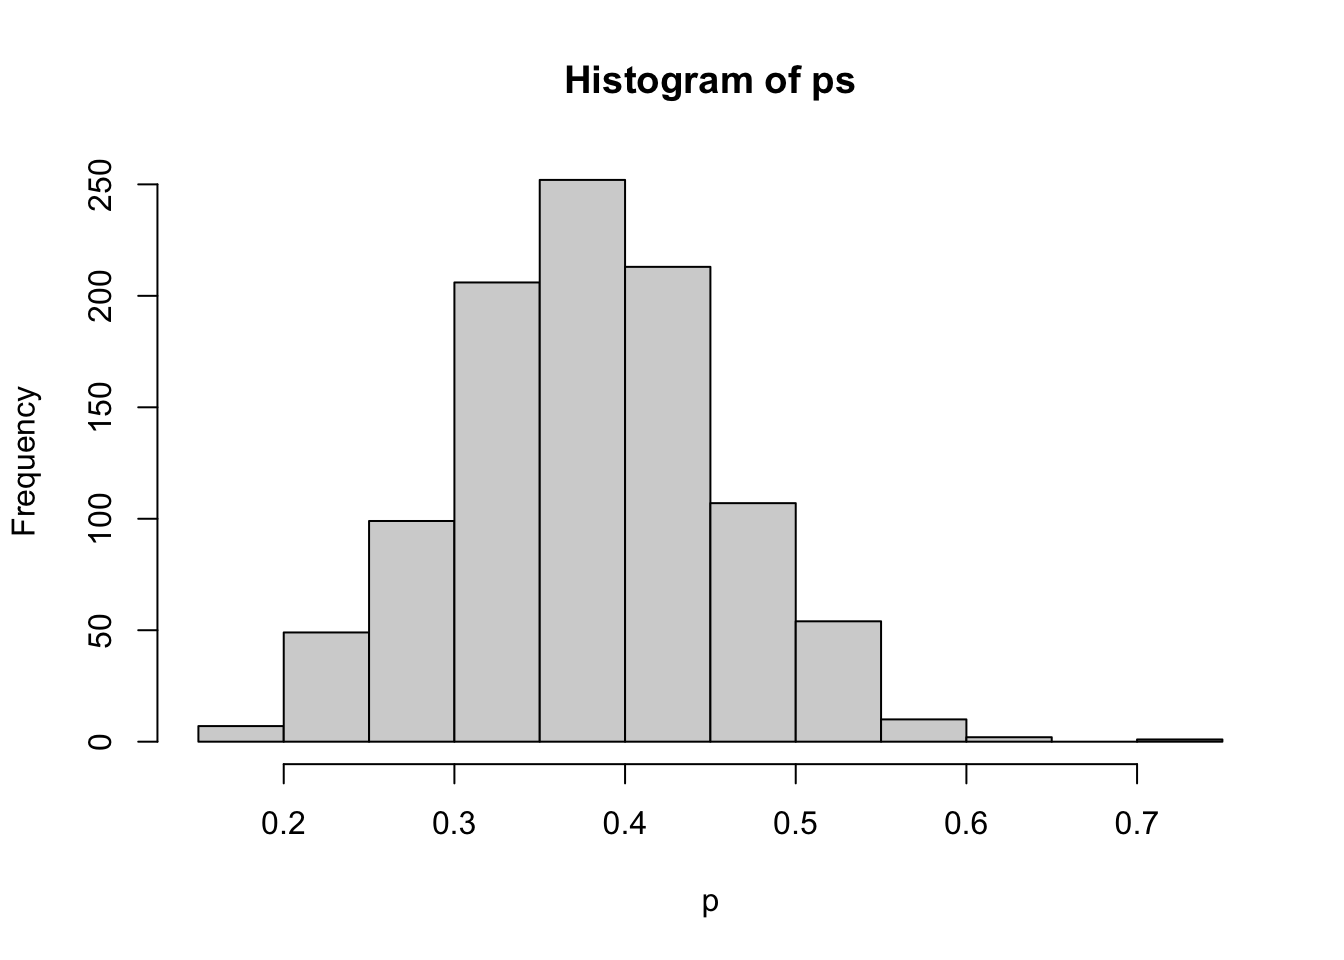
\includegraphics{bookdown-demo_files/figure-latex/unnamed-chunk-10-1.pdf}

\begin{Shaded}
\begin{Highlighting}[]
\FunctionTok{sum}\NormalTok{(ps }\SpecialCharTok{\textgreater{}=} \FloatTok{0.5}\NormalTok{) }\SpecialCharTok{/} \DecValTok{1000}
\end{Highlighting}
\end{Shaded}

\begin{verbatim}
## [1] 0.064
\end{verbatim}

\begin{Shaded}
\begin{Highlighting}[]
\FunctionTok{quantile}\NormalTok{(ps, }\FunctionTok{c}\NormalTok{(}\FloatTok{0.05}\NormalTok{, }\FloatTok{0.95}\NormalTok{))}
\end{Highlighting}
\end{Shaded}

\begin{verbatim}
##        5%       95% 
## 0.2530540 0.5124985
\end{verbatim}

\hypertarget{using-a-histogram-prior}{%
\section{Using a Histogram Prior}\label{using-a-histogram-prior}}

Beliefs about \(p\) are expressed by a histogram prior. Illustrate brute force method of computing the posterior.

\begin{Shaded}
\begin{Highlighting}[]
\NormalTok{midpt }\OtherTok{\textless{}{-}} \FunctionTok{seq}\NormalTok{(}\FloatTok{0.05}\NormalTok{, }\FloatTok{0.95}\NormalTok{, }\AttributeTok{by =} \FloatTok{0.1}\NormalTok{)}
\NormalTok{prior }\OtherTok{\textless{}{-}} \FunctionTok{c}\NormalTok{(}\DecValTok{1}\NormalTok{, }\FloatTok{5.2}\NormalTok{, }\DecValTok{8}\NormalTok{, }\FloatTok{7.2}\NormalTok{, }\FloatTok{4.6}\NormalTok{, }\FloatTok{2.1}\NormalTok{, }\FloatTok{0.7}\NormalTok{, }
           \FloatTok{0.1}\NormalTok{, }\DecValTok{0}\NormalTok{, }\DecValTok{0}\NormalTok{)}
\NormalTok{prior }\OtherTok{\textless{}{-}}\NormalTok{ prior }\SpecialCharTok{/} \FunctionTok{sum}\NormalTok{(prior)}
\end{Highlighting}
\end{Shaded}

\begin{Shaded}
\begin{Highlighting}[]
\FunctionTok{curve}\NormalTok{(}\FunctionTok{histprior}\NormalTok{(x, midpt, prior), }\AttributeTok{from=}\DecValTok{0}\NormalTok{, }\AttributeTok{to=}\DecValTok{1}\NormalTok{,}
   \AttributeTok{ylab=}\StringTok{"Prior density"}\NormalTok{, }\AttributeTok{ylim=}\FunctionTok{c}\NormalTok{(}\DecValTok{0}\NormalTok{, .}\DecValTok{3}\NormalTok{))}
\end{Highlighting}
\end{Shaded}

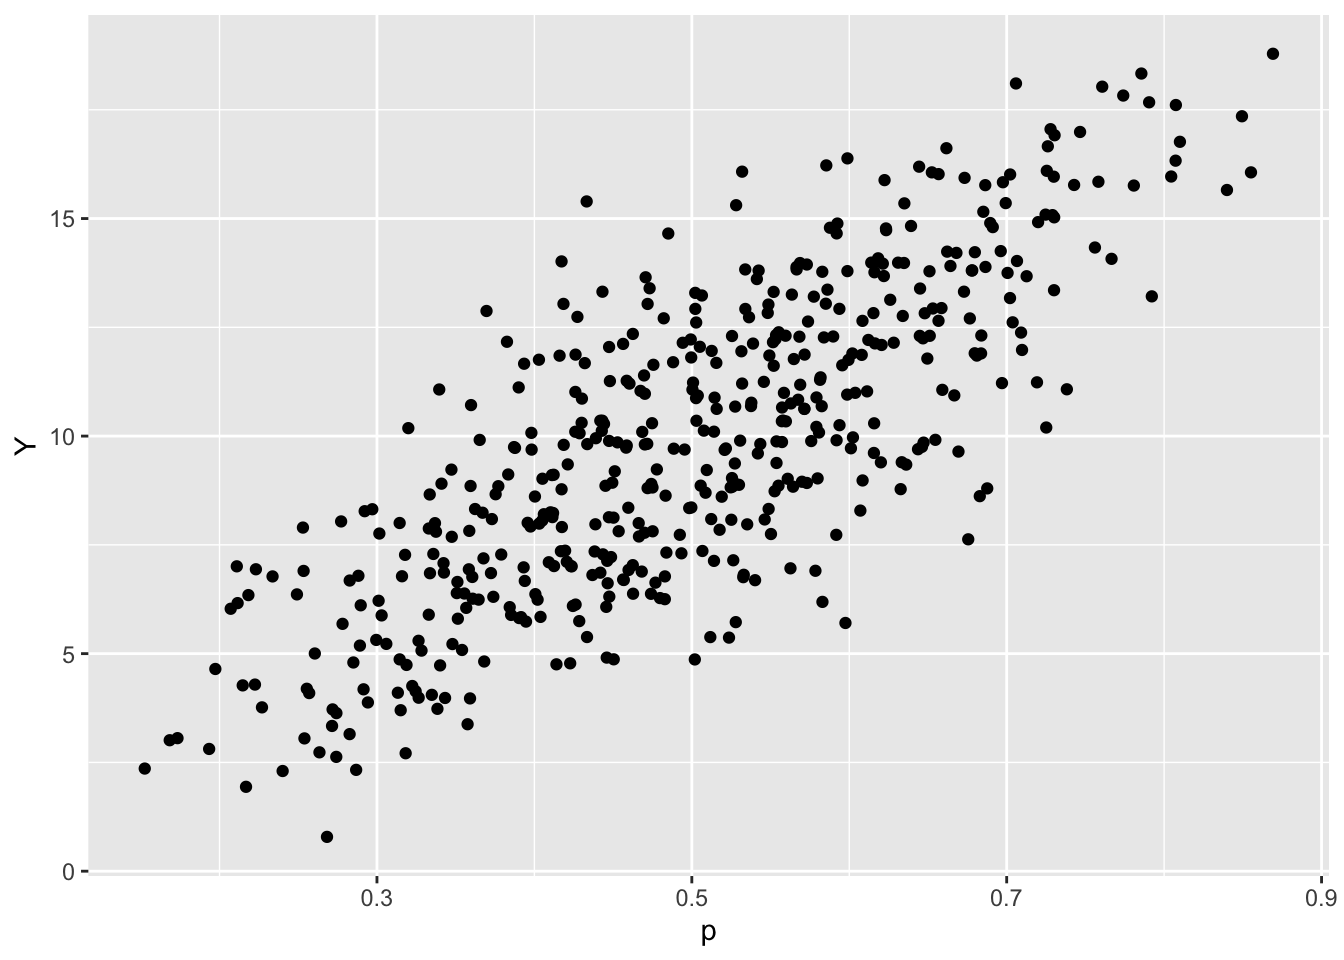
\includegraphics{bookdown-demo_files/figure-latex/unnamed-chunk-14-1.pdf}

\begin{Shaded}
\begin{Highlighting}[]
\NormalTok{s }\OtherTok{\textless{}{-}} \DecValTok{11}
\NormalTok{f }\OtherTok{\textless{}{-}} \DecValTok{16}
\end{Highlighting}
\end{Shaded}

\begin{Shaded}
\begin{Highlighting}[]
\FunctionTok{curve}\NormalTok{(}\FunctionTok{histprior}\NormalTok{(x,midpt,prior) }\SpecialCharTok{*} 
        \FunctionTok{dbeta}\NormalTok{(x, s }\SpecialCharTok{+} \DecValTok{1}\NormalTok{, f }\SpecialCharTok{+} \DecValTok{1}\NormalTok{), }
   \AttributeTok{from=}\DecValTok{0}\NormalTok{, }\AttributeTok{to=}\DecValTok{1}\NormalTok{, }\AttributeTok{ylab=}\StringTok{"Posterior density"}\NormalTok{)}
\end{Highlighting}
\end{Shaded}

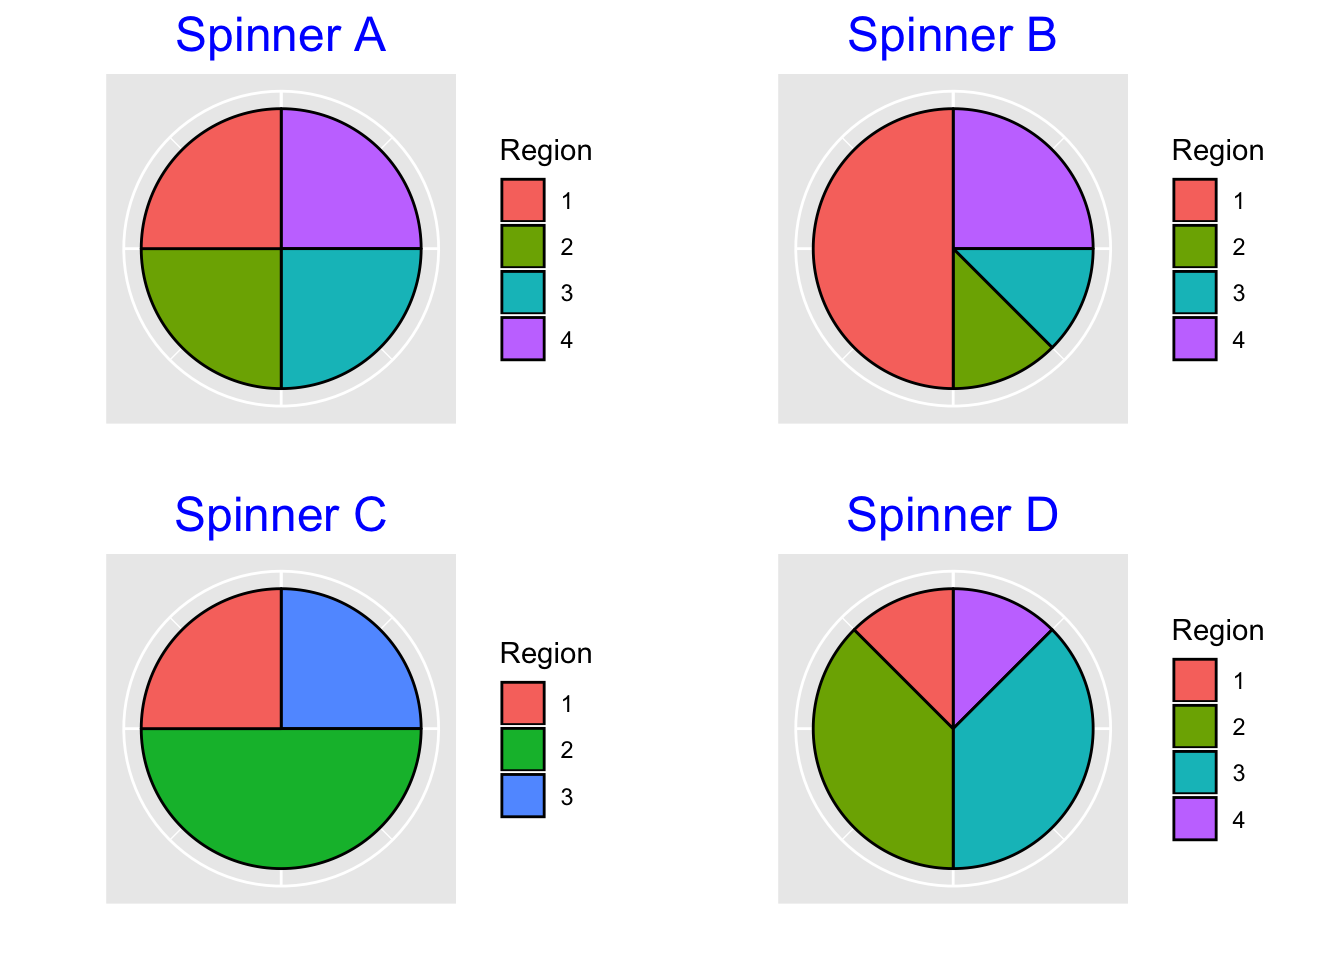
\includegraphics{bookdown-demo_files/figure-latex/unnamed-chunk-16-1.pdf}

\begin{Shaded}
\begin{Highlighting}[]
\NormalTok{p }\OtherTok{\textless{}{-}} \FunctionTok{seq}\NormalTok{(}\DecValTok{0}\NormalTok{, }\DecValTok{1}\NormalTok{, }\AttributeTok{length=}\DecValTok{500}\NormalTok{)}
\NormalTok{post }\OtherTok{\textless{}{-}} \FunctionTok{histprior}\NormalTok{(p, midpt, prior) }\SpecialCharTok{*}
        \FunctionTok{dbeta}\NormalTok{(p, s }\SpecialCharTok{+} \DecValTok{1}\NormalTok{, f }\SpecialCharTok{+} \DecValTok{1}\NormalTok{)}
\NormalTok{post }\OtherTok{\textless{}{-}}\NormalTok{ post }\SpecialCharTok{/} \FunctionTok{sum}\NormalTok{(post)}
\NormalTok{ps }\OtherTok{\textless{}{-}} \FunctionTok{sample}\NormalTok{(p, }\AttributeTok{replace =} \ConstantTok{TRUE}\NormalTok{, }\AttributeTok{prob =}\NormalTok{ post)}
\end{Highlighting}
\end{Shaded}

\begin{Shaded}
\begin{Highlighting}[]
\FunctionTok{hist}\NormalTok{(ps, }\AttributeTok{xlab=}\StringTok{"p"}\NormalTok{, }\AttributeTok{main=}\StringTok{""}\NormalTok{)}
\end{Highlighting}
\end{Shaded}

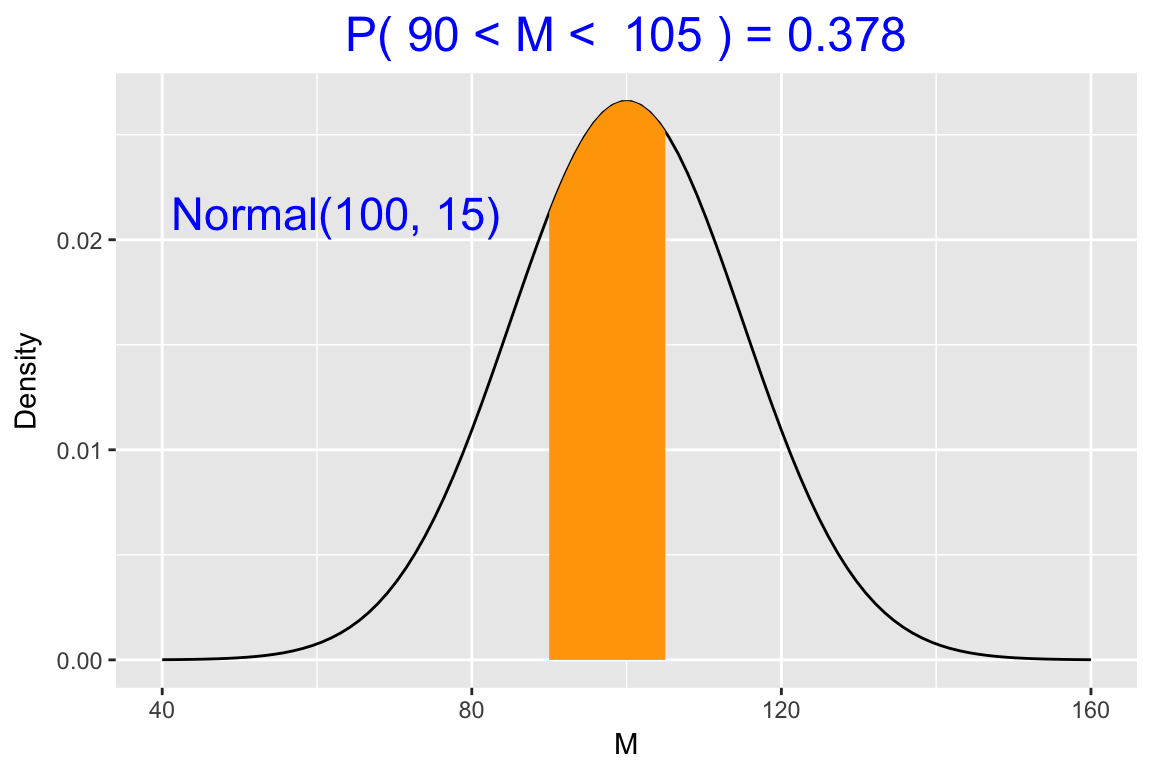
\includegraphics{bookdown-demo_files/figure-latex/unnamed-chunk-18-1.pdf}

\hypertarget{prediction}{%
\section{Prediction}\label{prediction}}

Want to predict the number of heavy sleepers in a future sample of 20.

Discrete prior approach:

\begin{Shaded}
\begin{Highlighting}[]
\NormalTok{p }\OtherTok{\textless{}{-}} \FunctionTok{seq}\NormalTok{(}\FloatTok{0.05}\NormalTok{, }\FloatTok{0.95}\NormalTok{, }\AttributeTok{by=}\NormalTok{.}\DecValTok{1}\NormalTok{)}
\NormalTok{prior }\OtherTok{\textless{}{-}} \FunctionTok{c}\NormalTok{(}\DecValTok{1}\NormalTok{, }\FloatTok{5.2}\NormalTok{, }\DecValTok{8}\NormalTok{, }\FloatTok{7.2}\NormalTok{, }\FloatTok{4.6}\NormalTok{, }
           \FloatTok{2.1}\NormalTok{, }\FloatTok{0.7}\NormalTok{, }\FloatTok{0.1}\NormalTok{, }\DecValTok{0}\NormalTok{, }\DecValTok{0}\NormalTok{)}
\NormalTok{prior }\OtherTok{\textless{}{-}}\NormalTok{ prior }\SpecialCharTok{/} \FunctionTok{sum}\NormalTok{(prior)}
\NormalTok{m }\OtherTok{\textless{}{-}} \DecValTok{20}
\NormalTok{ys }\OtherTok{\textless{}{-}} \DecValTok{0}\SpecialCharTok{:}\DecValTok{20}
\NormalTok{pred }\OtherTok{\textless{}{-}} \FunctionTok{pdiscp}\NormalTok{(p, prior, m, ys)}
\FunctionTok{cbind}\NormalTok{(}\DecValTok{0}\SpecialCharTok{:}\DecValTok{20}\NormalTok{, pred)}
\end{Highlighting}
\end{Shaded}

\begin{verbatim}
##                  pred
##  [1,]  0 2.030242e-02
##  [2,]  1 4.402694e-02
##  [3,]  2 6.894572e-02
##  [4,]  3 9.151046e-02
##  [5,]  4 1.064393e-01
##  [6,]  5 1.124487e-01
##  [7,]  6 1.104993e-01
##  [8,]  7 1.021397e-01
##  [9,]  8 8.932837e-02
## [10,]  9 7.416372e-02
## [11,] 10 5.851740e-02
## [12,] 11 4.383668e-02
## [13,] 12 3.107700e-02
## [14,] 13 2.071698e-02
## [15,] 14 1.284467e-02
## [16,] 15 7.277453e-03
## [17,] 16 3.667160e-03
## [18,] 17 1.575535e-03
## [19,] 18 5.381536e-04
## [20,] 19 1.285179e-04
## [21,] 20 1.584793e-05
\end{verbatim}

Continuous prior approach:

\begin{Shaded}
\begin{Highlighting}[]
\NormalTok{ab }\OtherTok{\textless{}{-}} \FunctionTok{c}\NormalTok{(}\FloatTok{3.26}\NormalTok{, }\FloatTok{7.19}\NormalTok{)}
\NormalTok{m }\OtherTok{\textless{}{-}} \DecValTok{20}
\NormalTok{ys }\OtherTok{\textless{}{-}} \DecValTok{0}\SpecialCharTok{:}\DecValTok{20}
\NormalTok{pred }\OtherTok{\textless{}{-}} \FunctionTok{pbetap}\NormalTok{(ab, m, ys)}
\end{Highlighting}
\end{Shaded}

Simulating predictive distribution:

\begin{Shaded}
\begin{Highlighting}[]
\NormalTok{p }\OtherTok{\textless{}{-}} \FunctionTok{rbeta}\NormalTok{(}\DecValTok{1000}\NormalTok{, }\FloatTok{3.26}\NormalTok{, }\FloatTok{7.19}\NormalTok{)}
\end{Highlighting}
\end{Shaded}

\begin{Shaded}
\begin{Highlighting}[]
\NormalTok{y }\OtherTok{\textless{}{-}} \FunctionTok{rbinom}\NormalTok{(}\DecValTok{1000}\NormalTok{, }\DecValTok{20}\NormalTok{, p)}
\end{Highlighting}
\end{Shaded}

\begin{Shaded}
\begin{Highlighting}[]
\FunctionTok{table}\NormalTok{(y)}
\end{Highlighting}
\end{Shaded}

\begin{verbatim}
## y
##   0   1   2   3   4   5   6   7   8   9  10  11  12  13  14  15  16  18  19 
##  11  52  70 101 105 102 116 100  84  67  47  50  32  20  21   9  10   2   1
\end{verbatim}

\begin{Shaded}
\begin{Highlighting}[]
\NormalTok{freq }\OtherTok{\textless{}{-}} \FunctionTok{table}\NormalTok{(y)}
\NormalTok{ys }\OtherTok{\textless{}{-}} \FunctionTok{as.integer}\NormalTok{(}\FunctionTok{names}\NormalTok{(freq))}
\NormalTok{predprob }\OtherTok{\textless{}{-}}\NormalTok{ freq }\SpecialCharTok{/} \FunctionTok{sum}\NormalTok{(freq)}
\FunctionTok{plot}\NormalTok{(ys, predprob, }\AttributeTok{type=}\StringTok{"h"}\NormalTok{, }\AttributeTok{xlab=}\StringTok{"y"}\NormalTok{,}
   \AttributeTok{ylab=}\StringTok{"Predictive Probability"}\NormalTok{)}
\end{Highlighting}
\end{Shaded}

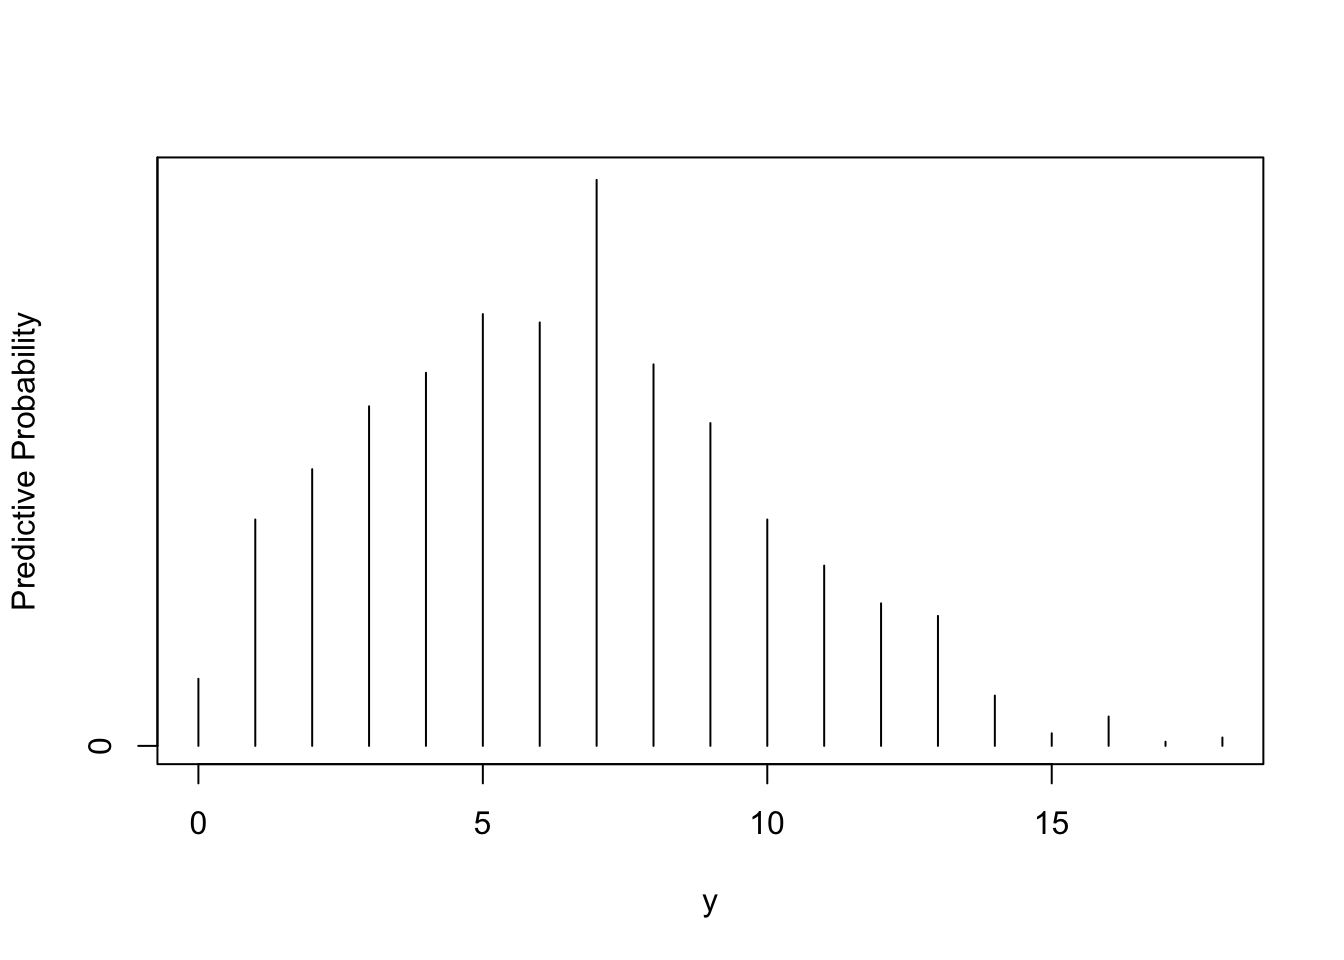
\includegraphics{bookdown-demo_files/figure-latex/unnamed-chunk-24-1.pdf}

\begin{Shaded}
\begin{Highlighting}[]
\NormalTok{dist }\OtherTok{\textless{}{-}} \FunctionTok{cbind}\NormalTok{(ys, predprob)}
\end{Highlighting}
\end{Shaded}

Construction of a prediction interval:

\begin{Shaded}
\begin{Highlighting}[]
\NormalTok{covprob }\OtherTok{\textless{}{-}}\NormalTok{ .}\DecValTok{9}
\FunctionTok{discint}\NormalTok{(dist, covprob)}
\end{Highlighting}
\end{Shaded}

\begin{verbatim}
## $prob
##    12 
## 0.926 
## 
## $set
##  1  2  3  4  5  6  7  8  9 10 11 12 
##  1  2  3  4  5  6  7  8  9 10 11 12
\end{verbatim}

\hypertarget{single-parameter-models}{%
\chapter{Single-Parameter Models}\label{single-parameter-models}}

\hypertarget{normal-distribution-with-known-mean-but-unknown-variance}{%
\section{Normal Distribution with Known Mean but Unknown Variance}\label{normal-distribution-with-known-mean-but-unknown-variance}}

Assuming we have a sample \{\(y_j\)\} from a normal distribution with mean 0 and variance \(\sigma^2\). Assuming the prior \(g(\sigma^2) \propto 1/\sigma^2\), simulating from the posterior.

\begin{Shaded}
\begin{Highlighting}[]
\FunctionTok{library}\NormalTok{(LearnBayes)}
\end{Highlighting}
\end{Shaded}

\begin{Shaded}
\begin{Highlighting}[]
\NormalTok{d }\OtherTok{\textless{}{-}} \FunctionTok{with}\NormalTok{(footballscores,}
\NormalTok{          favorite }\SpecialCharTok{{-}}\NormalTok{ underdog }\SpecialCharTok{{-}}\NormalTok{ spread)}
\NormalTok{n }\OtherTok{\textless{}{-}} \FunctionTok{length}\NormalTok{(d)}
\NormalTok{v }\OtherTok{\textless{}{-}} \FunctionTok{sum}\NormalTok{(d }\SpecialCharTok{\^{}} \DecValTok{2}\NormalTok{)}
\end{Highlighting}
\end{Shaded}

\begin{Shaded}
\begin{Highlighting}[]
\NormalTok{P }\OtherTok{\textless{}{-}} \FunctionTok{rchisq}\NormalTok{(}\DecValTok{1000}\NormalTok{, n) }\SpecialCharTok{/}\NormalTok{ v}
\NormalTok{s }\OtherTok{\textless{}{-}} \FunctionTok{sqrt}\NormalTok{(}\DecValTok{1} \SpecialCharTok{/}\NormalTok{ P)}
\FunctionTok{hist}\NormalTok{(s)}
\end{Highlighting}
\end{Shaded}

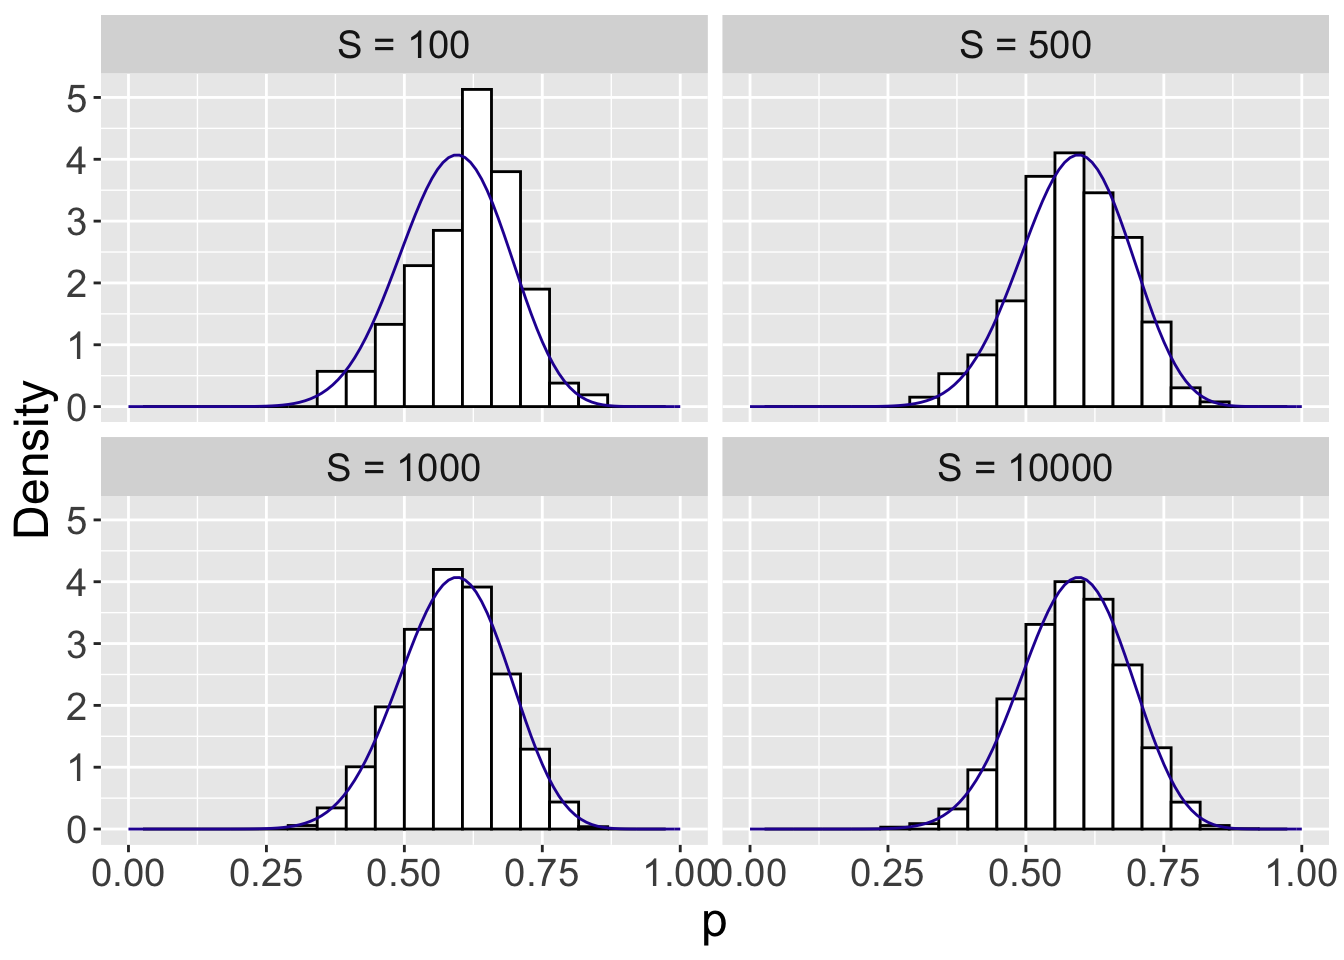
\includegraphics{bookdown-demo_files/figure-latex/unnamed-chunk-29-1.pdf}

\begin{Shaded}
\begin{Highlighting}[]
\FunctionTok{quantile}\NormalTok{(s, }\AttributeTok{probs =} \FunctionTok{c}\NormalTok{(}\FloatTok{0.025}\NormalTok{, }\FloatTok{0.5}\NormalTok{, }\FloatTok{0.975}\NormalTok{))}
\end{Highlighting}
\end{Shaded}

\begin{verbatim}
##     2.5%      50%    97.5% 
## 13.16744 13.85293 14.60743
\end{verbatim}

\hypertarget{estimating-a-heart-transplant-mortality-rate}{%
\section{Estimating a Heart Transplant Mortality Rate}\label{estimating-a-heart-transplant-mortality-rate}}

Have a sample \{\(y_j\)\} from a Poisson(\(e \lambda\)) distribution where the exposure \(e\) is known. Assigning \(\lambda\) a gamma(\(\alpha, \beta\)) prior.

Predictive density:

\begin{Shaded}
\begin{Highlighting}[]
\NormalTok{alpha }\OtherTok{\textless{}{-}} \DecValTok{16}\NormalTok{; beta }\OtherTok{\textless{}{-}} \DecValTok{15174}
\NormalTok{yobs }\OtherTok{\textless{}{-}} \DecValTok{1}\NormalTok{; ex }\OtherTok{\textless{}{-}} \DecValTok{66}
\NormalTok{y }\OtherTok{\textless{}{-}} \DecValTok{0}\SpecialCharTok{:}\DecValTok{10}
\NormalTok{lam }\OtherTok{\textless{}{-}}\NormalTok{ alpha }\SpecialCharTok{/}\NormalTok{ beta}
\NormalTok{py }\OtherTok{\textless{}{-}} \FunctionTok{dpois}\NormalTok{(y, lam }\SpecialCharTok{*}\NormalTok{ ex) }\SpecialCharTok{*} 
  \FunctionTok{dgamma}\NormalTok{(lam, }\AttributeTok{shape =}\NormalTok{ alpha, }\AttributeTok{rate =}\NormalTok{ beta) }\SpecialCharTok{/} 
  \FunctionTok{dgamma}\NormalTok{(lam, }\AttributeTok{shape =}\NormalTok{ alpha }\SpecialCharTok{+}\NormalTok{ y, }\AttributeTok{rate =}\NormalTok{ beta }\SpecialCharTok{+}\NormalTok{ ex)}
\FunctionTok{cbind}\NormalTok{(y, }\FunctionTok{round}\NormalTok{(py, }\DecValTok{3}\NormalTok{))}
\end{Highlighting}
\end{Shaded}

\begin{verbatim}
##        y      
##  [1,]  0 0.933
##  [2,]  1 0.065
##  [3,]  2 0.002
##  [4,]  3 0.000
##  [5,]  4 0.000
##  [6,]  5 0.000
##  [7,]  6 0.000
##  [8,]  7 0.000
##  [9,]  8 0.000
## [10,]  9 0.000
## [11,] 10 0.000
\end{verbatim}

Posterior density:

\begin{Shaded}
\begin{Highlighting}[]
\NormalTok{lambdaA }\OtherTok{\textless{}{-}} \FunctionTok{rgamma}\NormalTok{(}\DecValTok{1000}\NormalTok{, }\AttributeTok{shape =}\NormalTok{ alpha }\SpecialCharTok{+}\NormalTok{ yobs, }
                  \AttributeTok{rate =}\NormalTok{ beta }\SpecialCharTok{+}\NormalTok{ ex)}
\end{Highlighting}
\end{Shaded}

Data from a different hospital:

\begin{Shaded}
\begin{Highlighting}[]
\NormalTok{ex }\OtherTok{\textless{}{-}} \DecValTok{1767}\NormalTok{; yobs }\OtherTok{\textless{}{-}}\DecValTok{4}
\NormalTok{y }\OtherTok{\textless{}{-}} \DecValTok{0}\SpecialCharTok{:}\DecValTok{10}
\NormalTok{py }\OtherTok{\textless{}{-}} \FunctionTok{dpois}\NormalTok{(y, lam }\SpecialCharTok{*}\NormalTok{ ex) }\SpecialCharTok{*} 
  \FunctionTok{dgamma}\NormalTok{(lam, }\AttributeTok{shape =}\NormalTok{ alpha, }\AttributeTok{rate =}\NormalTok{ beta) }\SpecialCharTok{/}   
  \FunctionTok{dgamma}\NormalTok{(lam, }\AttributeTok{shape =}\NormalTok{ alpha }\SpecialCharTok{+}\NormalTok{ y, }\AttributeTok{rate =}\NormalTok{ beta }\SpecialCharTok{+}\NormalTok{ ex)}
 \FunctionTok{cbind}\NormalTok{(y, }\FunctionTok{round}\NormalTok{(py, }\DecValTok{3}\NormalTok{))}
\end{Highlighting}
\end{Shaded}

\begin{verbatim}
##        y      
##  [1,]  0 0.172
##  [2,]  1 0.286
##  [3,]  2 0.254
##  [4,]  3 0.159
##  [5,]  4 0.079
##  [6,]  5 0.033
##  [7,]  6 0.012
##  [8,]  7 0.004
##  [9,]  8 0.001
## [10,]  9 0.000
## [11,] 10 0.000
\end{verbatim}

\begin{Shaded}
\begin{Highlighting}[]
\NormalTok{lambdaB }\OtherTok{\textless{}{-}} \FunctionTok{rgamma}\NormalTok{(}\DecValTok{1000}\NormalTok{, }\AttributeTok{shape =}\NormalTok{ alpha }\SpecialCharTok{+}\NormalTok{ yobs,}
                  \AttributeTok{rate =}\NormalTok{ beta }\SpecialCharTok{+}\NormalTok{ ex)}
\end{Highlighting}
\end{Shaded}

Prior and posteriors for two hospitals:

\begin{Shaded}
\begin{Highlighting}[]
\FunctionTok{par}\NormalTok{(}\AttributeTok{mfrow =} \FunctionTok{c}\NormalTok{(}\DecValTok{2}\NormalTok{, }\DecValTok{1}\NormalTok{))}
 \FunctionTok{plot}\NormalTok{(}\FunctionTok{density}\NormalTok{(lambdaA), }\AttributeTok{main=}\StringTok{"HOSPITAL A"}\NormalTok{,}
      \AttributeTok{xlab=}\StringTok{"lambdaA"}\NormalTok{, }\AttributeTok{lwd=}\DecValTok{3}\NormalTok{)}
 \FunctionTok{curve}\NormalTok{(}\FunctionTok{dgamma}\NormalTok{(x, }\AttributeTok{shape =}\NormalTok{ alpha, }\AttributeTok{rate =}\NormalTok{ beta),}
       \AttributeTok{add=}\ConstantTok{TRUE}\NormalTok{)}
 \FunctionTok{legend}\NormalTok{(}\StringTok{"topright"}\NormalTok{,}\AttributeTok{legend=}\FunctionTok{c}\NormalTok{(}\StringTok{"prior"}\NormalTok{,}\StringTok{"posterior"}\NormalTok{),}
        \AttributeTok{lwd=}\FunctionTok{c}\NormalTok{(}\DecValTok{1}\NormalTok{,}\DecValTok{3}\NormalTok{))}
 \FunctionTok{plot}\NormalTok{(}\FunctionTok{density}\NormalTok{(lambdaB), }\AttributeTok{main=}\StringTok{"HOSPITAL B"}\NormalTok{,}
      \AttributeTok{xlab=}\StringTok{"lambdaB"}\NormalTok{, }\AttributeTok{lwd=}\DecValTok{3}\NormalTok{)}
 \FunctionTok{curve}\NormalTok{(}\FunctionTok{dgamma}\NormalTok{(x, }\AttributeTok{shape =}\NormalTok{ alpha, }\AttributeTok{rate =}\NormalTok{ beta),}
       \AttributeTok{add=}\ConstantTok{TRUE}\NormalTok{)}
 \FunctionTok{legend}\NormalTok{(}\StringTok{"topright"}\NormalTok{,}\AttributeTok{legend=}\FunctionTok{c}\NormalTok{(}\StringTok{"prior"}\NormalTok{,}\StringTok{"posterior"}\NormalTok{),}
        \AttributeTok{lwd=}\FunctionTok{c}\NormalTok{(}\DecValTok{1}\NormalTok{,}\DecValTok{3}\NormalTok{))}
\end{Highlighting}
\end{Shaded}

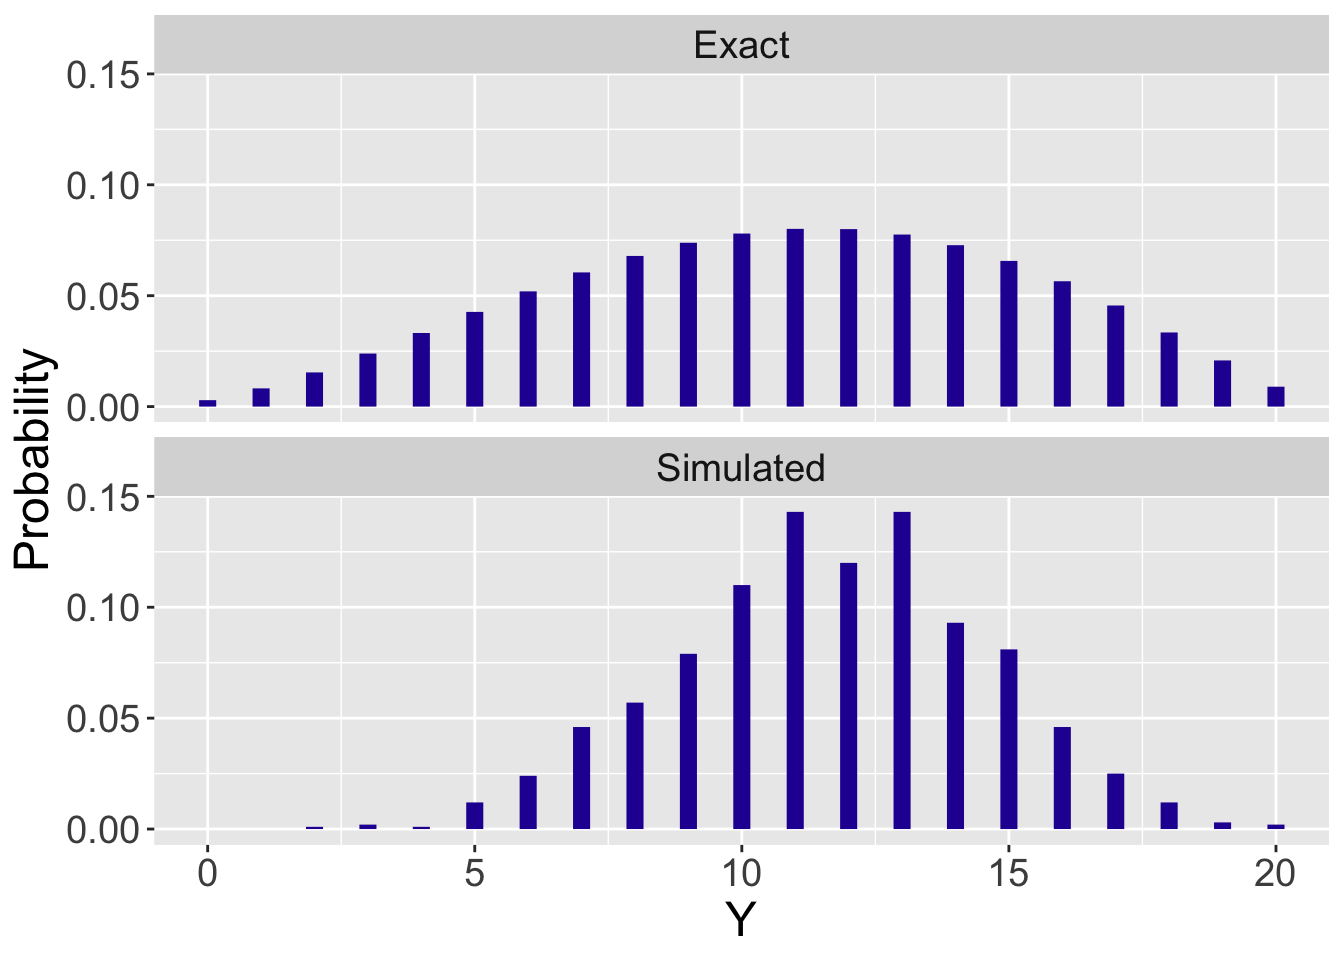
\includegraphics{bookdown-demo_files/figure-latex/unnamed-chunk-35-1.pdf}

\hypertarget{an-illustration-of-bayesian-robustness}{%
\section{An Illustration of Bayesian Robustness}\label{an-illustration-of-bayesian-robustness}}

Assuming normal sampling (known standard deviation), compare the use of two priors on the mean \(\mu\).

\begin{Shaded}
\begin{Highlighting}[]
\NormalTok{quantile1 }\OtherTok{\textless{}{-}} \FunctionTok{list}\NormalTok{(}\AttributeTok{p=}\NormalTok{.}\DecValTok{5}\NormalTok{, }\AttributeTok{x=}\DecValTok{100}\NormalTok{)}
\NormalTok{quantile2 }\OtherTok{\textless{}{-}} \FunctionTok{list}\NormalTok{(}\AttributeTok{p=}\NormalTok{.}\DecValTok{95}\NormalTok{, }\AttributeTok{x=}\DecValTok{120}\NormalTok{)}
\FunctionTok{normal.select}\NormalTok{(quantile1, quantile2)}
\end{Highlighting}
\end{Shaded}

\begin{verbatim}
## $mu
## [1] 100
## 
## $sigma
## [1] 12.15914
\end{verbatim}

\begin{Shaded}
\begin{Highlighting}[]
\NormalTok{mu }\OtherTok{\textless{}{-}} \DecValTok{100}
\NormalTok{tau }\OtherTok{\textless{}{-}} \FloatTok{12.16}
\NormalTok{sigma }\OtherTok{\textless{}{-}} \DecValTok{15}
\NormalTok{n }\OtherTok{\textless{}{-}} \DecValTok{4}
\NormalTok{se }\OtherTok{\textless{}{-}}\NormalTok{ sigma }\SpecialCharTok{/} \FunctionTok{sqrt}\NormalTok{(}\DecValTok{4}\NormalTok{)}
\NormalTok{ybar }\OtherTok{\textless{}{-}} \FunctionTok{c}\NormalTok{(}\DecValTok{110}\NormalTok{, }\DecValTok{125}\NormalTok{, }\DecValTok{140}\NormalTok{)}
\NormalTok{tau1 }\OtherTok{\textless{}{-}} \DecValTok{1} \SpecialCharTok{/} \FunctionTok{sqrt}\NormalTok{(}\DecValTok{1} \SpecialCharTok{/}\NormalTok{ se }\SpecialCharTok{\^{}} \DecValTok{2} \SpecialCharTok{+} \DecValTok{1} \SpecialCharTok{/}\NormalTok{ tau }\SpecialCharTok{\^{}} \DecValTok{2}\NormalTok{)}
\NormalTok{mu1 }\OtherTok{\textless{}{-}}\NormalTok{ (ybar }\SpecialCharTok{/}\NormalTok{ se }\SpecialCharTok{\^{}} \DecValTok{2} \SpecialCharTok{+}\NormalTok{ mu }\SpecialCharTok{/}\NormalTok{ tau }\SpecialCharTok{\^{}} \DecValTok{2}\NormalTok{) }\SpecialCharTok{*}\NormalTok{ tau1 }\SpecialCharTok{\^{}} \DecValTok{2}
\NormalTok{summ1 }\OtherTok{\textless{}{-}} \FunctionTok{cbind}\NormalTok{(ybar, mu1, tau1)}
\NormalTok{summ1}
\end{Highlighting}
\end{Shaded}

\begin{verbatim}
##      ybar      mu1     tau1
## [1,]  110 107.2442 6.383469
## [2,]  125 118.1105 6.383469
## [3,]  140 128.9768 6.383469
\end{verbatim}

Compare two possible priors for \(\mu\):

\begin{Shaded}
\begin{Highlighting}[]
\NormalTok{tscale }\OtherTok{\textless{}{-}} \DecValTok{20} \SpecialCharTok{/} \FunctionTok{qt}\NormalTok{(}\FloatTok{0.95}\NormalTok{, }\DecValTok{2}\NormalTok{)}
\NormalTok{tscale}
\end{Highlighting}
\end{Shaded}

\begin{verbatim}
## [1] 6.849349
\end{verbatim}

\begin{Shaded}
\begin{Highlighting}[]
\FunctionTok{par}\NormalTok{(}\AttributeTok{mfrow=}\FunctionTok{c}\NormalTok{(}\DecValTok{1}\NormalTok{, }\DecValTok{1}\NormalTok{))}
\FunctionTok{curve}\NormalTok{(}\DecValTok{1} \SpecialCharTok{/}\NormalTok{ tscale }\SpecialCharTok{*} \FunctionTok{dt}\NormalTok{((x }\SpecialCharTok{{-}}\NormalTok{ mu) }\SpecialCharTok{/}\NormalTok{ tscale, }\DecValTok{2}\NormalTok{),}
   \AttributeTok{from=}\DecValTok{60}\NormalTok{, }\AttributeTok{to=}\DecValTok{140}\NormalTok{, }\AttributeTok{xlab=}\StringTok{"theta"}\NormalTok{, }
   \AttributeTok{ylab=}\StringTok{"Prior Density"}\NormalTok{)}
\FunctionTok{curve}\NormalTok{(}\FunctionTok{dnorm}\NormalTok{(x, }\AttributeTok{mean=}\NormalTok{mu, }\AttributeTok{sd=}\NormalTok{tau), }\AttributeTok{add=}\ConstantTok{TRUE}\NormalTok{, }\AttributeTok{lwd=}\DecValTok{3}\NormalTok{)}
\FunctionTok{legend}\NormalTok{(}\StringTok{"topright"}\NormalTok{, }\AttributeTok{legend=}\FunctionTok{c}\NormalTok{(}\StringTok{"t density"}\NormalTok{,}
                            \StringTok{"normal density"}\NormalTok{),}
       \AttributeTok{lwd=}\FunctionTok{c}\NormalTok{(}\DecValTok{1}\NormalTok{,}\DecValTok{3}\NormalTok{))}
\end{Highlighting}
\end{Shaded}

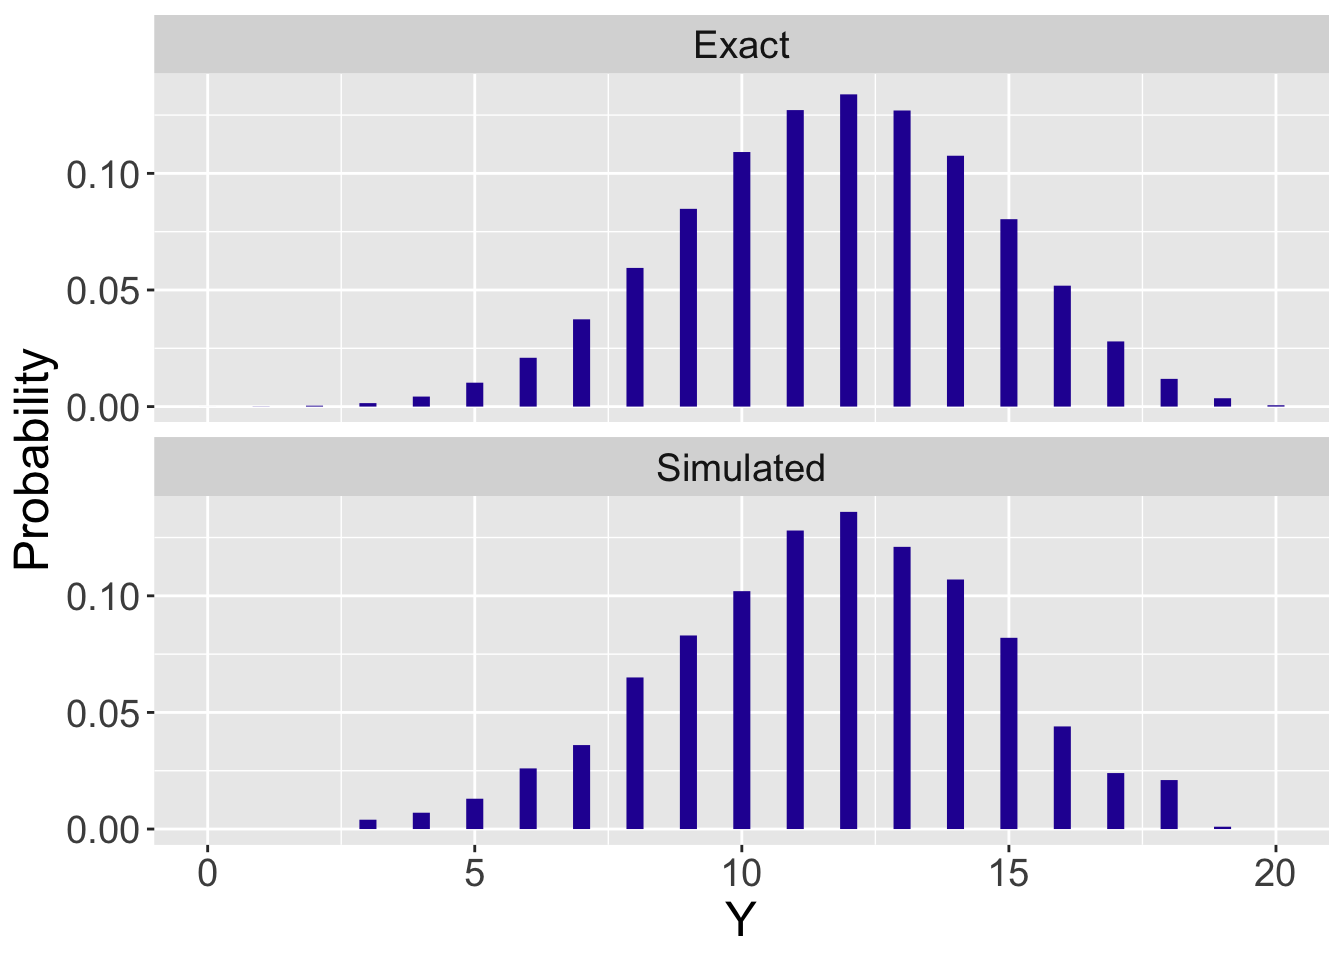
\includegraphics{bookdown-demo_files/figure-latex/unnamed-chunk-38-1.pdf}

\begin{Shaded}
\begin{Highlighting}[]
\NormalTok{norm.t.compute }\OtherTok{\textless{}{-}} \ControlFlowTok{function}\NormalTok{(ybar)\{}
\NormalTok{     theta }\OtherTok{\textless{}{-}} \FunctionTok{seq}\NormalTok{(}\DecValTok{60}\NormalTok{, }\DecValTok{180}\NormalTok{, }\AttributeTok{length =} \DecValTok{500}\NormalTok{)}
\NormalTok{     like }\OtherTok{\textless{}{-}} \FunctionTok{dnorm}\NormalTok{(theta, }\AttributeTok{mean=}\NormalTok{ybar,}
                   \AttributeTok{sd=}\NormalTok{sigma}\SpecialCharTok{/}\FunctionTok{sqrt}\NormalTok{(n))}
\NormalTok{     prior }\OtherTok{\textless{}{-}} \FunctionTok{dt}\NormalTok{((theta }\SpecialCharTok{{-}}\NormalTok{ mu) }\SpecialCharTok{/}\NormalTok{ tscale, }\DecValTok{2}\NormalTok{)}
\NormalTok{     post }\OtherTok{\textless{}{-}}\NormalTok{ prior }\SpecialCharTok{*}\NormalTok{ like}
\NormalTok{     post }\OtherTok{\textless{}{-}}\NormalTok{ post }\SpecialCharTok{/} \FunctionTok{sum}\NormalTok{(post)}
\NormalTok{     m }\OtherTok{\textless{}{-}} \FunctionTok{sum}\NormalTok{(theta }\SpecialCharTok{*}\NormalTok{ post)}
\NormalTok{     s }\OtherTok{\textless{}{-}} \FunctionTok{sqrt}\NormalTok{(}\FunctionTok{sum}\NormalTok{(theta }\SpecialCharTok{\^{}} \DecValTok{2} \SpecialCharTok{*}\NormalTok{ post) }\SpecialCharTok{{-}}\NormalTok{ m }\SpecialCharTok{\^{}} \DecValTok{2}\NormalTok{)}
     \FunctionTok{c}\NormalTok{(ybar, m, s) }
\NormalTok{\}}
\end{Highlighting}
\end{Shaded}

\begin{Shaded}
\begin{Highlighting}[]
\NormalTok{summ2 }\OtherTok{\textless{}{-}} \FunctionTok{t}\NormalTok{(}\FunctionTok{sapply}\NormalTok{(}\FunctionTok{c}\NormalTok{(}\DecValTok{110}\NormalTok{, }\DecValTok{125}\NormalTok{, }\DecValTok{140}\NormalTok{),}
\NormalTok{                  norm.t.compute))}
\FunctionTok{dimnames}\NormalTok{(summ2)[[}\DecValTok{2}\NormalTok{]] }\OtherTok{\textless{}{-}} \FunctionTok{c}\NormalTok{(}\StringTok{"ybar"}\NormalTok{, }\StringTok{"mu1 t"}\NormalTok{, }
                          \StringTok{"tau1 t"}\NormalTok{)}
\NormalTok{summ2}
\end{Highlighting}
\end{Shaded}

\begin{verbatim}
##      ybar    mu1 t   tau1 t
## [1,]  110 105.2921 5.841676
## [2,]  125 118.0841 7.885174
## [3,]  140 135.4134 7.973498
\end{verbatim}

\begin{Shaded}
\begin{Highlighting}[]
\FunctionTok{cbind}\NormalTok{(summ1, summ2)}
\end{Highlighting}
\end{Shaded}

\begin{verbatim}
##      ybar      mu1     tau1 ybar    mu1 t   tau1 t
## [1,]  110 107.2442 6.383469  110 105.2921 5.841676
## [2,]  125 118.1105 6.383469  125 118.0841 7.885174
## [3,]  140 128.9768 6.383469  140 135.4134 7.973498
\end{verbatim}

Compare two posterior densities:

\begin{Shaded}
\begin{Highlighting}[]
\NormalTok{theta }\OtherTok{\textless{}{-}} \FunctionTok{seq}\NormalTok{(}\DecValTok{60}\NormalTok{, }\DecValTok{180}\NormalTok{, }\AttributeTok{length=}\DecValTok{500}\NormalTok{)}
\NormalTok{normpost }\OtherTok{\textless{}{-}} \FunctionTok{dnorm}\NormalTok{(theta, mu1[}\DecValTok{3}\NormalTok{], tau1)}
\NormalTok{normpost }\OtherTok{\textless{}{-}}\NormalTok{ normpost }\SpecialCharTok{/} \FunctionTok{sum}\NormalTok{(normpost)}
\FunctionTok{plot}\NormalTok{(theta, normpost, }\AttributeTok{type=}\StringTok{"l"}\NormalTok{, }\AttributeTok{lwd=}\DecValTok{3}\NormalTok{,}
     \AttributeTok{ylab=}\StringTok{"Posterior Density"}\NormalTok{)}
\NormalTok{like }\OtherTok{\textless{}{-}} \FunctionTok{dnorm}\NormalTok{(theta, }\AttributeTok{mean=}\DecValTok{140}\NormalTok{, }\AttributeTok{sd=}\NormalTok{sigma }\SpecialCharTok{/} \FunctionTok{sqrt}\NormalTok{(n))}
\NormalTok{prior }\OtherTok{\textless{}{-}} \FunctionTok{dt}\NormalTok{((theta }\SpecialCharTok{{-}}\NormalTok{ mu) }\SpecialCharTok{/}\NormalTok{ tscale, }\DecValTok{2}\NormalTok{)}
\NormalTok{tpost }\OtherTok{\textless{}{-}}\NormalTok{ prior }\SpecialCharTok{*}\NormalTok{ like }\SpecialCharTok{/} \FunctionTok{sum}\NormalTok{(prior }\SpecialCharTok{*}\NormalTok{ like)  }
\FunctionTok{lines}\NormalTok{(theta, tpost)}
\FunctionTok{legend}\NormalTok{(}\StringTok{"topright"}\NormalTok{, }\AttributeTok{legend=}\FunctionTok{c}\NormalTok{(}\StringTok{"t prior"}\NormalTok{, }
                            \StringTok{"normal prior"}\NormalTok{), }
       \AttributeTok{lwd=}\FunctionTok{c}\NormalTok{(}\DecValTok{1}\NormalTok{,}\DecValTok{3}\NormalTok{))}
\end{Highlighting}
\end{Shaded}

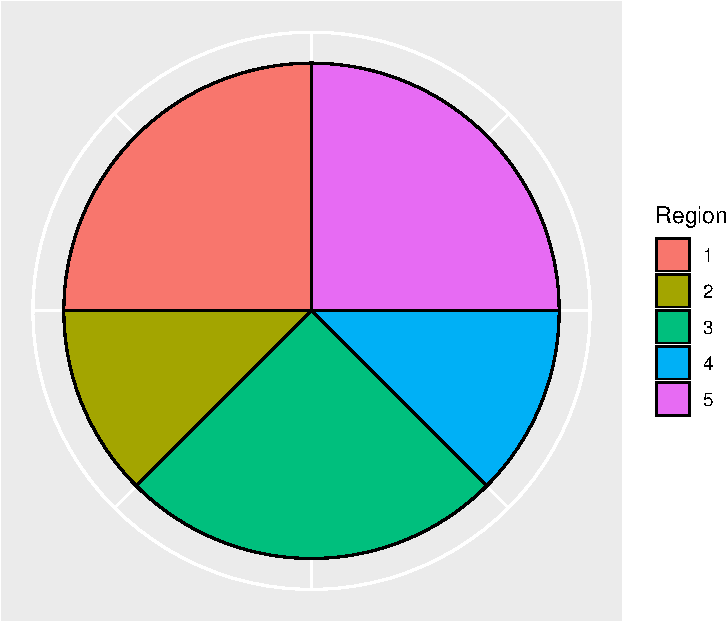
\includegraphics{bookdown-demo_files/figure-latex/unnamed-chunk-42-1.pdf}

\hypertarget{mixtures-of-conjugate-priors}{%
\section{Mixtures of Conjugate Priors}\label{mixtures-of-conjugate-priors}}

Use a mixture of beta curves to reflect beliefs that a particular coin is biased.

\begin{Shaded}
\begin{Highlighting}[]
\FunctionTok{curve}\NormalTok{(.}\DecValTok{5} \SpecialCharTok{*} \FunctionTok{dbeta}\NormalTok{(x, }\DecValTok{6}\NormalTok{, }\DecValTok{14}\NormalTok{) }\SpecialCharTok{+}\NormalTok{ .}\DecValTok{5} \SpecialCharTok{*} \FunctionTok{dbeta}\NormalTok{(x, }\DecValTok{14}\NormalTok{, }\DecValTok{6}\NormalTok{),}
      \AttributeTok{from=}\DecValTok{0}\NormalTok{, }\AttributeTok{to=}\DecValTok{1}\NormalTok{, }\AttributeTok{xlab=}\StringTok{"P"}\NormalTok{, }\AttributeTok{ylab=}\StringTok{"Density"}\NormalTok{)}
\end{Highlighting}
\end{Shaded}

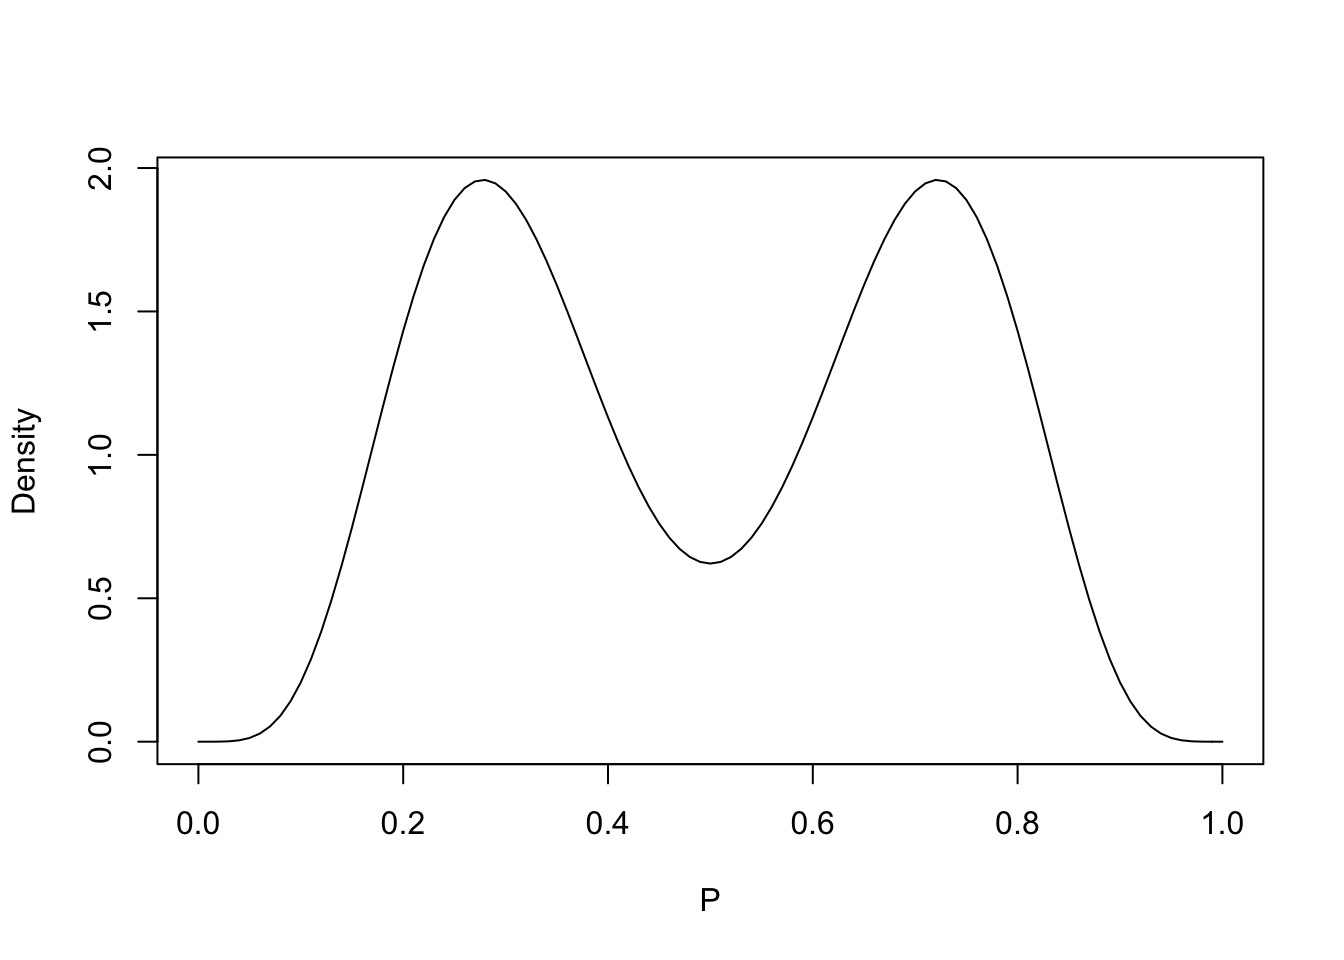
\includegraphics{bookdown-demo_files/figure-latex/unnamed-chunk-43-1.pdf}

\begin{Shaded}
\begin{Highlighting}[]
\NormalTok{probs }\OtherTok{\textless{}{-}} \FunctionTok{c}\NormalTok{(.}\DecValTok{5}\NormalTok{, .}\DecValTok{5}\NormalTok{)}
\NormalTok{beta.par1 }\OtherTok{\textless{}{-}} \FunctionTok{c}\NormalTok{(}\DecValTok{6}\NormalTok{, }\DecValTok{14}\NormalTok{)}
\NormalTok{beta.par2 }\OtherTok{\textless{}{-}} \FunctionTok{c}\NormalTok{(}\DecValTok{14}\NormalTok{, }\DecValTok{6}\NormalTok{)}
\NormalTok{betapar }\OtherTok{\textless{}{-}} \FunctionTok{rbind}\NormalTok{(beta.par1, beta.par2)}
\NormalTok{data }\OtherTok{\textless{}{-}} \FunctionTok{c}\NormalTok{(}\DecValTok{7}\NormalTok{, }\DecValTok{3}\NormalTok{)}
\NormalTok{post }\OtherTok{\textless{}{-}} \FunctionTok{binomial.beta.mix}\NormalTok{(probs, betapar, data)}
\NormalTok{post}
\end{Highlighting}
\end{Shaded}

\begin{verbatim}
## $probs
##  beta.par1  beta.par2 
## 0.09269663 0.90730337 
## 
## $betapar
##           [,1] [,2]
## beta.par1   13   17
## beta.par2   21    9
\end{verbatim}

Compare prior and posterior densities for the probability coin lands heads.

\begin{Shaded}
\begin{Highlighting}[]
\FunctionTok{curve}\NormalTok{(post}\SpecialCharTok{$}\NormalTok{probs[}\DecValTok{1}\NormalTok{] }\SpecialCharTok{*} \FunctionTok{dbeta}\NormalTok{(x,}\DecValTok{13}\NormalTok{,}\DecValTok{17}\NormalTok{) }\SpecialCharTok{+}
\NormalTok{        post}\SpecialCharTok{$}\NormalTok{probs[}\DecValTok{2}\NormalTok{] }\SpecialCharTok{*} \FunctionTok{dbeta}\NormalTok{(x,}\DecValTok{21}\NormalTok{,}\DecValTok{9}\NormalTok{),}
  \AttributeTok{from=}\DecValTok{0}\NormalTok{, }\AttributeTok{to=}\DecValTok{1}\NormalTok{, }\AttributeTok{lwd=}\DecValTok{3}\NormalTok{, }
  \AttributeTok{xlab=}\StringTok{"P"}\NormalTok{, }\AttributeTok{ylab=}\StringTok{"DENSITY"}\NormalTok{)}
\FunctionTok{curve}\NormalTok{(.}\DecValTok{5} \SpecialCharTok{*} \FunctionTok{dbeta}\NormalTok{(x, }\DecValTok{6}\NormalTok{, }\DecValTok{12}\NormalTok{) }\SpecialCharTok{+} 
\NormalTok{        .}\DecValTok{5} \SpecialCharTok{*} \FunctionTok{dbeta}\NormalTok{(x, }\DecValTok{12}\NormalTok{, }\DecValTok{6}\NormalTok{), }\DecValTok{0}\NormalTok{, }\DecValTok{1}\NormalTok{, }\AttributeTok{add=}\ConstantTok{TRUE}\NormalTok{)}
\FunctionTok{legend}\NormalTok{(}\StringTok{"topleft"}\NormalTok{, }\AttributeTok{legend=}\FunctionTok{c}\NormalTok{(}\StringTok{"Prior"}\NormalTok{, }\StringTok{"Posterior"}\NormalTok{),}
       \AttributeTok{lwd=}\FunctionTok{c}\NormalTok{(}\DecValTok{1}\NormalTok{, }\DecValTok{3}\NormalTok{))}
\end{Highlighting}
\end{Shaded}

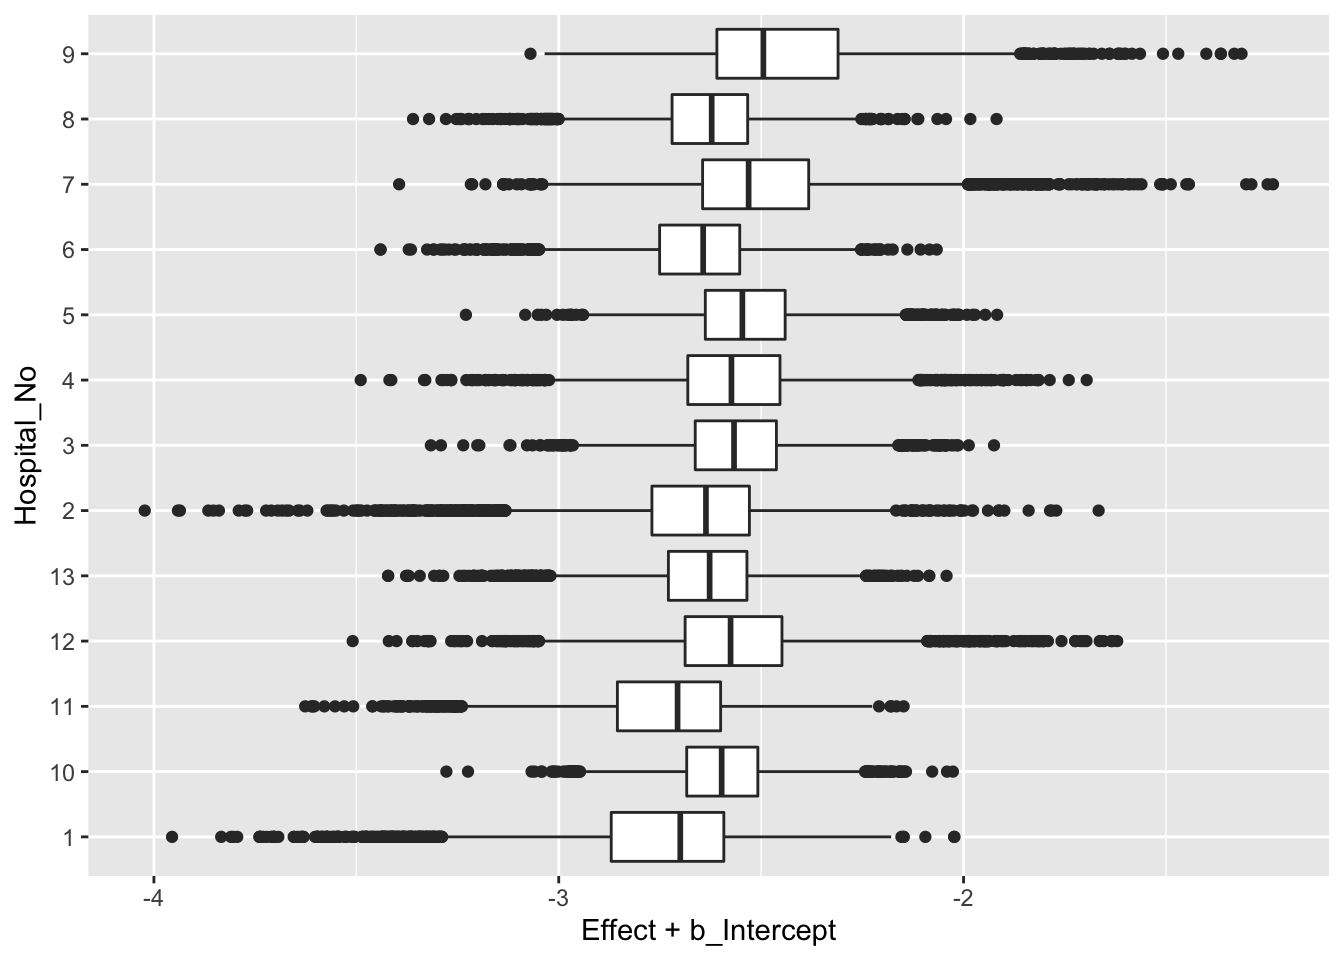
\includegraphics{bookdown-demo_files/figure-latex/unnamed-chunk-45-1.pdf}

\hypertarget{a-bayesian-test-of-the-fairness-of-a-coin}{%
\section{A Bayesian Test of the Fairness of a Coin}\label{a-bayesian-test-of-the-fairness-of-a-coin}}

Testing if a coin is fair. Observe 5 heads in 20 flips.

P-value calculation:

\begin{Shaded}
\begin{Highlighting}[]
\FunctionTok{pbinom}\NormalTok{(}\DecValTok{5}\NormalTok{, }\DecValTok{20}\NormalTok{, }\FloatTok{0.5}\NormalTok{)}
\end{Highlighting}
\end{Shaded}

\begin{verbatim}
## [1] 0.02069473
\end{verbatim}

Bayesian test of fairness using a mixture prior.

\begin{Shaded}
\begin{Highlighting}[]
\NormalTok{n }\OtherTok{\textless{}{-}} \DecValTok{20}
\NormalTok{y }\OtherTok{\textless{}{-}} \DecValTok{5}
\NormalTok{a }\OtherTok{\textless{}{-}} \DecValTok{10}
\NormalTok{p }\OtherTok{\textless{}{-}} \FloatTok{0.5}
\NormalTok{m1 }\OtherTok{\textless{}{-}} \FunctionTok{dbinom}\NormalTok{(y, n, p) }\SpecialCharTok{*} \FunctionTok{dbeta}\NormalTok{(p, a, a) }\SpecialCharTok{/} 
  \FunctionTok{dbeta}\NormalTok{(p, a }\SpecialCharTok{+}\NormalTok{ y, a }\SpecialCharTok{+}\NormalTok{ n }\SpecialCharTok{{-}}\NormalTok{ y)}
\NormalTok{lambda }\OtherTok{\textless{}{-}} \FunctionTok{dbinom}\NormalTok{(y, n, p) }\SpecialCharTok{/}\NormalTok{ (}\FunctionTok{dbinom}\NormalTok{(y, n, p) }\SpecialCharTok{+}\NormalTok{ m1)}
\NormalTok{lambda}
\end{Highlighting}
\end{Shaded}

\begin{verbatim}
## [1] 0.2802215
\end{verbatim}

\begin{Shaded}
\begin{Highlighting}[]
\FunctionTok{pbetat}\NormalTok{(p, .}\DecValTok{5}\NormalTok{, }\FunctionTok{c}\NormalTok{(a, a), }\FunctionTok{c}\NormalTok{(y, n }\SpecialCharTok{{-}}\NormalTok{ y))}
\end{Highlighting}
\end{Shaded}

\begin{verbatim}
## $bf
## [1] 0.3893163
## 
## $post
## [1] 0.2802215
\end{verbatim}

\begin{Shaded}
\begin{Highlighting}[]
\NormalTok{prob.fair }\OtherTok{\textless{}{-}} \ControlFlowTok{function}\NormalTok{(log.a)\{}
\NormalTok{  a }\OtherTok{\textless{}{-}} \FunctionTok{exp}\NormalTok{(log.a)}
\NormalTok{  m2 }\OtherTok{\textless{}{-}} \FunctionTok{dbinom}\NormalTok{(y, n, p) }\SpecialCharTok{*} \FunctionTok{dbeta}\NormalTok{(p, a, a) }\SpecialCharTok{/}
             \FunctionTok{dbeta}\NormalTok{(p, a }\SpecialCharTok{+}\NormalTok{ y, a }\SpecialCharTok{+}\NormalTok{ n }\SpecialCharTok{{-}}\NormalTok{ y)}
  \FunctionTok{dbinom}\NormalTok{(y, n, p) }\SpecialCharTok{/}\NormalTok{ (}\FunctionTok{dbinom}\NormalTok{(y, n, p) }\SpecialCharTok{+}\NormalTok{ m2)}
\NormalTok{\}}
\end{Highlighting}
\end{Shaded}

\begin{Shaded}
\begin{Highlighting}[]
\NormalTok{n }\OtherTok{\textless{}{-}} \DecValTok{20}\NormalTok{; y }\OtherTok{\textless{}{-}} \DecValTok{5}\NormalTok{; p }\OtherTok{\textless{}{-}} \FloatTok{0.5}
\FunctionTok{curve}\NormalTok{(}\FunctionTok{prob.fair}\NormalTok{(x), }\AttributeTok{from =} \SpecialCharTok{{-}}\DecValTok{4}\NormalTok{, }\AttributeTok{to =} \DecValTok{5}\NormalTok{, }
      \AttributeTok{xlab=}\StringTok{"log a"}\NormalTok{, }
      \AttributeTok{ylab=}\StringTok{"Prob(coin is fair)"}\NormalTok{, }\AttributeTok{lwd=}\DecValTok{2}\NormalTok{)}
\end{Highlighting}
\end{Shaded}

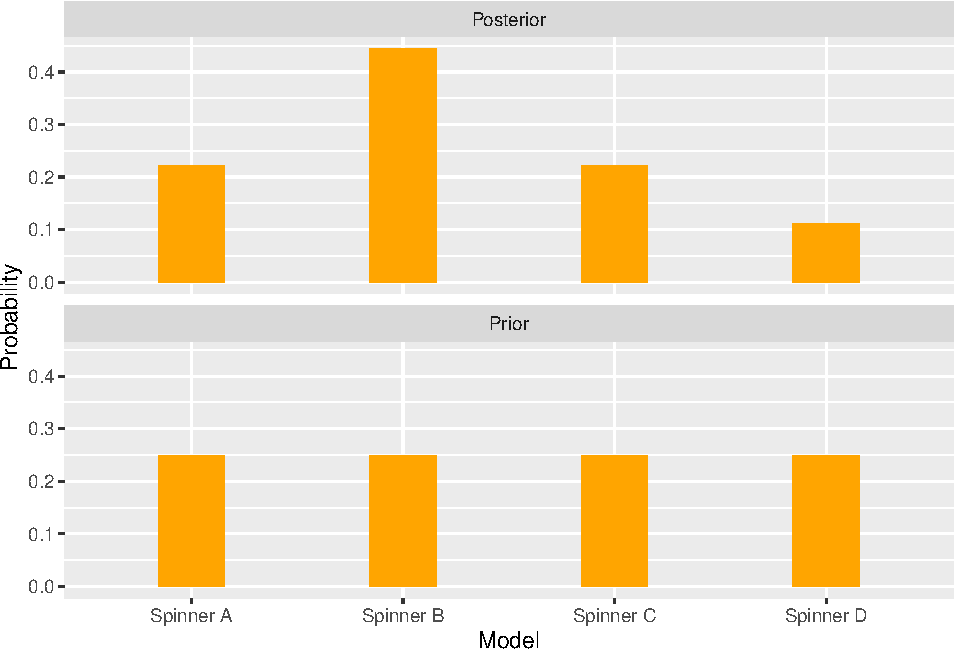
\includegraphics{bookdown-demo_files/figure-latex/unnamed-chunk-50-1.pdf}

\begin{Shaded}
\begin{Highlighting}[]
\NormalTok{n }\OtherTok{\textless{}{-}} \DecValTok{20}\NormalTok{; y }\OtherTok{\textless{}{-}} \DecValTok{5}
\NormalTok{a }\OtherTok{\textless{}{-}} \DecValTok{10}\NormalTok{; p }\OtherTok{\textless{}{-}}\NormalTok{ .}\DecValTok{5}
\NormalTok{m2 }\OtherTok{\textless{}{-}} \DecValTok{0}
 \ControlFlowTok{for}\NormalTok{ (k }\ControlFlowTok{in} \DecValTok{0}\SpecialCharTok{:}\NormalTok{y)\{}
\NormalTok{   m2 }\OtherTok{\textless{}{-}}\NormalTok{ m2 }\SpecialCharTok{+} \FunctionTok{dbinom}\NormalTok{(k, n, p) }\SpecialCharTok{*} \FunctionTok{dbeta}\NormalTok{(p, a, a) }\SpecialCharTok{/}
     \FunctionTok{dbeta}\NormalTok{(p, a }\SpecialCharTok{+}\NormalTok{ k, a }\SpecialCharTok{+}\NormalTok{ n }\SpecialCharTok{{-}}\NormalTok{ k)}
\NormalTok{\}}
\NormalTok{lambda }\OtherTok{\textless{}{-}} \FunctionTok{pbinom}\NormalTok{(y, n, p) }\SpecialCharTok{/}\NormalTok{ (}\FunctionTok{pbinom}\NormalTok{(y, n, p) }\SpecialCharTok{+}\NormalTok{ m2)}
\NormalTok{lambda}
\end{Highlighting}
\end{Shaded}

\begin{verbatim}
## [1] 0.2184649
\end{verbatim}

\hypertarget{multiparameter-models}{%
\chapter{Multiparameter Models}\label{multiparameter-models}}

\hypertarget{normal-data-with-both-parameters-unknown}{%
\section{Normal Data with Both Parameters Unknown}\label{normal-data-with-both-parameters-unknown}}

Illustrates exact posterior sampling of (\(\mu, \sigma^2\)) for normal sampling with a noninformative prior.

\begin{Shaded}
\begin{Highlighting}[]
\FunctionTok{library}\NormalTok{(LearnBayes)}
\end{Highlighting}
\end{Shaded}

\begin{Shaded}
\begin{Highlighting}[]
\FunctionTok{mycontour}\NormalTok{(normchi2post, }
               \FunctionTok{c}\NormalTok{(}\DecValTok{220}\NormalTok{, }\DecValTok{330}\NormalTok{, }\DecValTok{500}\NormalTok{, }\DecValTok{9000}\NormalTok{), }
\NormalTok{               marathontimes}\SpecialCharTok{$}\NormalTok{time,}
               \AttributeTok{xlab=}\StringTok{"mean"}\NormalTok{, }\AttributeTok{ylab=}\StringTok{"variance"}\NormalTok{)}
\end{Highlighting}
\end{Shaded}

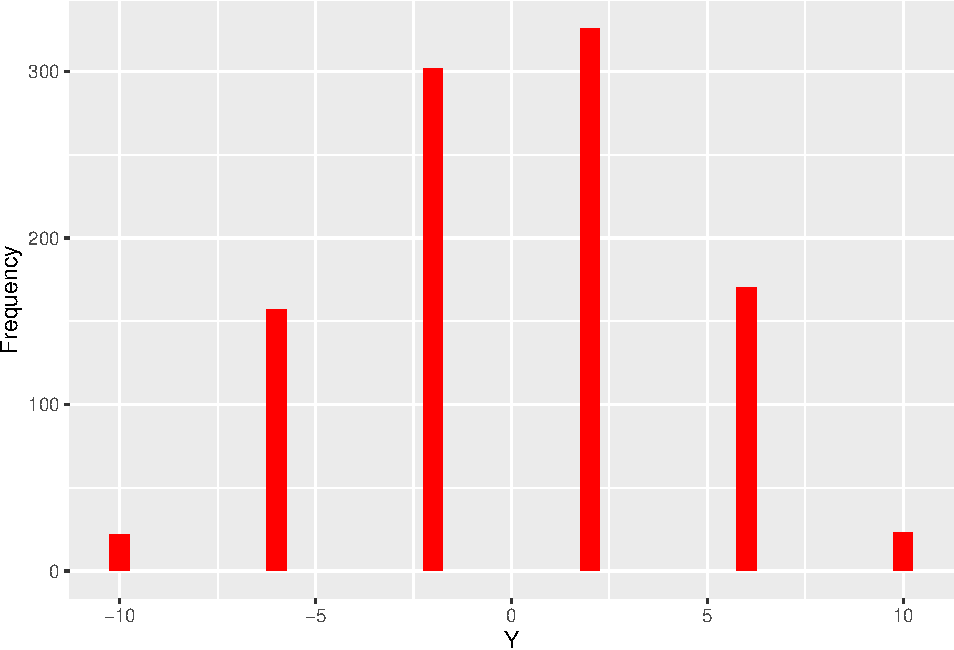
\includegraphics{bookdown-demo_files/figure-latex/unnamed-chunk-53-1.pdf}

\begin{Shaded}
\begin{Highlighting}[]
\NormalTok{S }\OtherTok{\textless{}{-}} \FunctionTok{with}\NormalTok{(marathontimes, }
          \FunctionTok{sum}\NormalTok{((time }\SpecialCharTok{{-}} \FunctionTok{mean}\NormalTok{(time))}\SpecialCharTok{\^{}}\DecValTok{2}\NormalTok{))}
\NormalTok{n }\OtherTok{\textless{}{-}} \FunctionTok{length}\NormalTok{(marathontimes}\SpecialCharTok{$}\NormalTok{time)}
\NormalTok{sigma2 }\OtherTok{\textless{}{-}}\NormalTok{ S }\SpecialCharTok{/} \FunctionTok{rchisq}\NormalTok{(}\DecValTok{1000}\NormalTok{, n }\SpecialCharTok{{-}} \DecValTok{1}\NormalTok{)}
\NormalTok{mu }\OtherTok{\textless{}{-}} \FunctionTok{rnorm}\NormalTok{(}\DecValTok{1000}\NormalTok{, }\AttributeTok{mean =} \FunctionTok{mean}\NormalTok{(marathontimes}\SpecialCharTok{$}\NormalTok{time),}
            \AttributeTok{sd =} \FunctionTok{sqrt}\NormalTok{(sigma2) }\SpecialCharTok{/} \FunctionTok{sqrt}\NormalTok{(n))}
\FunctionTok{mycontour}\NormalTok{(normchi2post, }
               \FunctionTok{c}\NormalTok{(}\DecValTok{220}\NormalTok{, }\DecValTok{330}\NormalTok{, }\DecValTok{500}\NormalTok{, }\DecValTok{9000}\NormalTok{), }
\NormalTok{               marathontimes}\SpecialCharTok{$}\NormalTok{time,}
               \AttributeTok{xlab=}\StringTok{"mean"}\NormalTok{, }\AttributeTok{ylab=}\StringTok{"variance"}\NormalTok{)}
\FunctionTok{points}\NormalTok{(mu, sigma2)}
\end{Highlighting}
\end{Shaded}

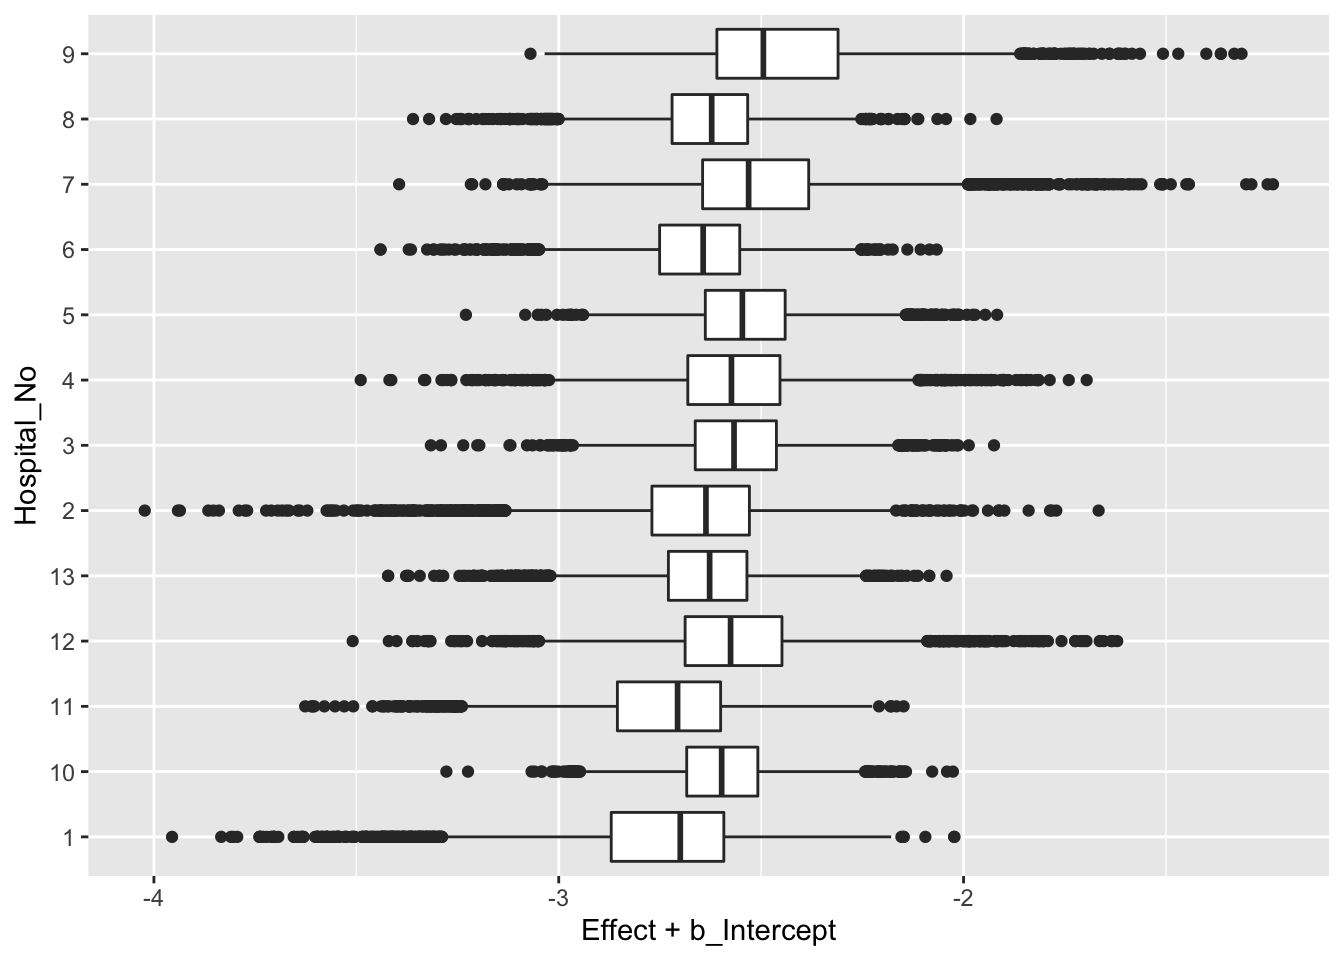
\includegraphics{bookdown-demo_files/figure-latex/unnamed-chunk-54-1.pdf}

\begin{Shaded}
\begin{Highlighting}[]
\FunctionTok{quantile}\NormalTok{(mu, }\FunctionTok{c}\NormalTok{(}\FloatTok{0.025}\NormalTok{, }\FloatTok{0.975}\NormalTok{))}
\end{Highlighting}
\end{Shaded}

\begin{verbatim}
##     2.5%    97.5% 
## 256.7045 301.1136
\end{verbatim}

\begin{Shaded}
\begin{Highlighting}[]
\FunctionTok{quantile}\NormalTok{(}\FunctionTok{sqrt}\NormalTok{(sigma2), }\FunctionTok{c}\NormalTok{(}\FloatTok{0.025}\NormalTok{, }\FloatTok{0.975}\NormalTok{))}
\end{Highlighting}
\end{Shaded}

\begin{verbatim}
##     2.5%    97.5% 
## 37.85306 73.41654
\end{verbatim}

\hypertarget{a-multinomial-model}{%
\section{A Multinomial Model}\label{a-multinomial-model}}

Multinomial data and a uniform prior placed on the proportions. Sampling from the Dirichlet posterior distribution.

\begin{Shaded}
\begin{Highlighting}[]
\NormalTok{alpha }\OtherTok{\textless{}{-}} \FunctionTok{c}\NormalTok{(}\DecValTok{728}\NormalTok{, }\DecValTok{584}\NormalTok{, }\DecValTok{138}\NormalTok{)}
\NormalTok{theta }\OtherTok{\textless{}{-}} \FunctionTok{rdirichlet}\NormalTok{(}\DecValTok{1000}\NormalTok{, alpha)}
\FunctionTok{hist}\NormalTok{(theta[, }\DecValTok{1}\NormalTok{] }\SpecialCharTok{{-}}\NormalTok{ theta[, }\DecValTok{2}\NormalTok{], }\AttributeTok{main=}\StringTok{""}\NormalTok{)}
\end{Highlighting}
\end{Shaded}

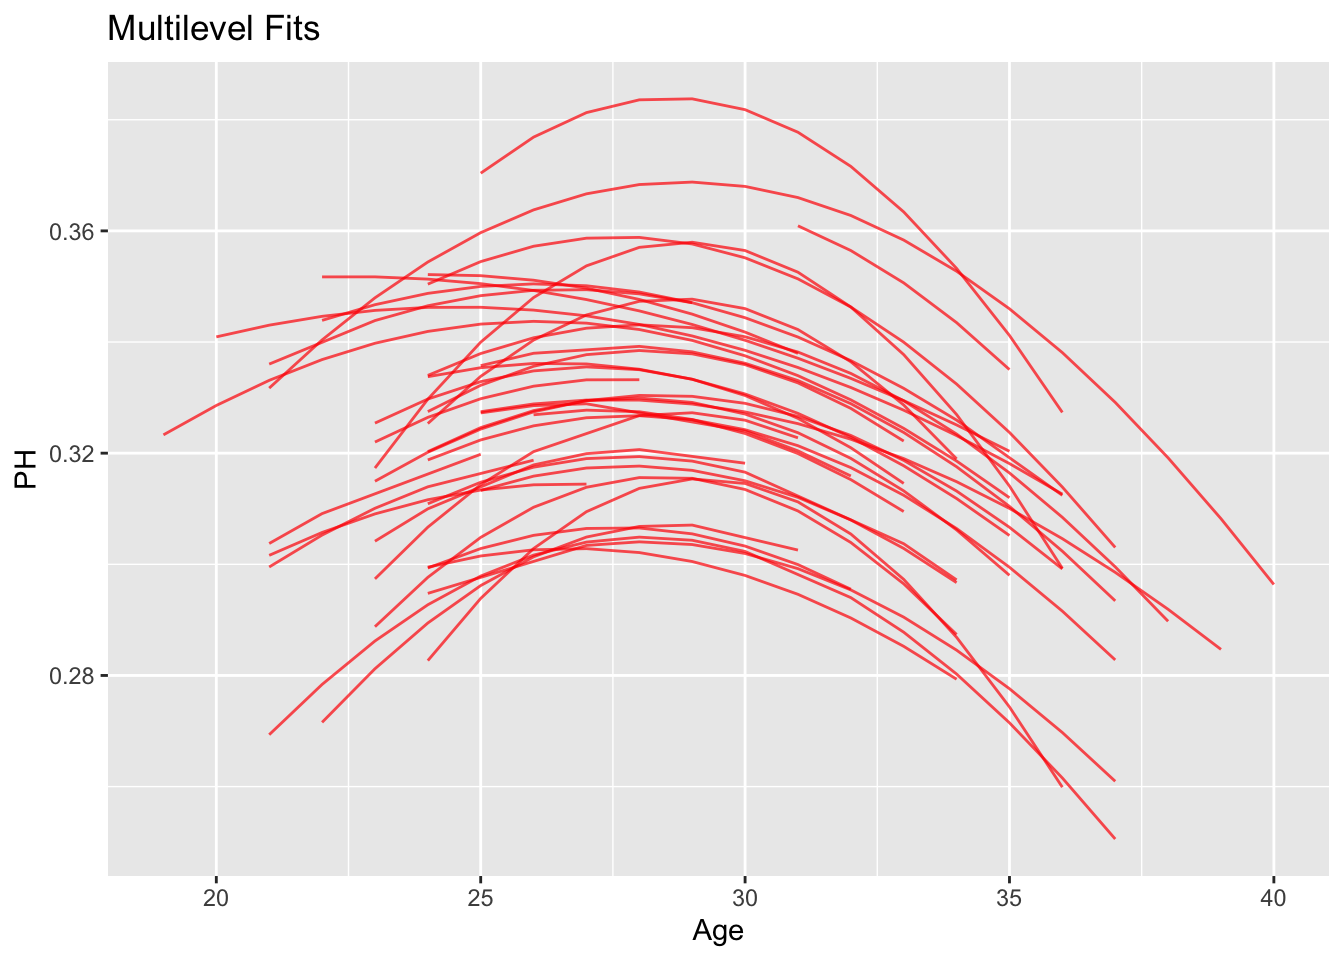
\includegraphics{bookdown-demo_files/figure-latex/unnamed-chunk-57-1.pdf}

Considers posterior distribution of Obama electoral votes for the 2008 presidential election.

\begin{Shaded}
\begin{Highlighting}[]
\NormalTok{prob.Obama }\OtherTok{\textless{}{-}} \ControlFlowTok{function}\NormalTok{(j)\{}
\NormalTok{  p }\OtherTok{\textless{}{-}} \FunctionTok{with}\NormalTok{(election}\FloatTok{.2008}\NormalTok{, }
            \FunctionTok{rdirichlet}\NormalTok{(}\DecValTok{5000}\NormalTok{,}
          \DecValTok{500} \SpecialCharTok{*} \FunctionTok{c}\NormalTok{(M.pct[j], O.pct[j], }
          \DecValTok{100} \SpecialCharTok{{-}}\NormalTok{ M.pct[j] }\SpecialCharTok{{-}}\NormalTok{ O.pct[j]) }\SpecialCharTok{/} \DecValTok{100} \SpecialCharTok{+} \DecValTok{1}\NormalTok{))}
  \FunctionTok{mean}\NormalTok{(p[, }\DecValTok{2}\NormalTok{] }\SpecialCharTok{\textgreater{}}\NormalTok{ p[, }\DecValTok{1}\NormalTok{])}
\NormalTok{\}}
\NormalTok{Obama.win.probs }\OtherTok{\textless{}{-}} \FunctionTok{sapply}\NormalTok{(}\DecValTok{1} \SpecialCharTok{:} \DecValTok{51}\NormalTok{, prob.Obama)}
\end{Highlighting}
\end{Shaded}

\begin{Shaded}
\begin{Highlighting}[]
\NormalTok{sim.election }\OtherTok{\textless{}{-}} \ControlFlowTok{function}\NormalTok{()\{}
\NormalTok{  winner }\OtherTok{\textless{}{-}} \FunctionTok{rbinom}\NormalTok{(}\DecValTok{51}\NormalTok{, }\DecValTok{1}\NormalTok{, }
\NormalTok{              Obama.win.probs)  }
  \FunctionTok{sum}\NormalTok{(election}\FloatTok{.2008}\SpecialCharTok{$}\NormalTok{EV }\SpecialCharTok{*}\NormalTok{ winner)         }
\NormalTok{\}}
\end{Highlighting}
\end{Shaded}

\begin{Shaded}
\begin{Highlighting}[]
\NormalTok{sim.EV }\OtherTok{\textless{}{-}} \FunctionTok{replicate}\NormalTok{(}\DecValTok{1000}\NormalTok{, }\FunctionTok{sim.election}\NormalTok{())}
\end{Highlighting}
\end{Shaded}

\begin{Shaded}
\begin{Highlighting}[]
\FunctionTok{hist}\NormalTok{(sim.EV, }\FunctionTok{min}\NormalTok{(sim.EV) }\SpecialCharTok{:} \FunctionTok{max}\NormalTok{(sim.EV), }\AttributeTok{col=}\StringTok{"blue"}\NormalTok{)}
\FunctionTok{abline}\NormalTok{(}\AttributeTok{v=}\DecValTok{365}\NormalTok{, }\AttributeTok{lwd=}\DecValTok{3}\NormalTok{)  }\CommentTok{\# Obama received 365 votes}
\FunctionTok{text}\NormalTok{(}\DecValTok{375}\NormalTok{, }\DecValTok{30}\NormalTok{, }\StringTok{"Actual }\SpecialCharTok{\textbackslash{}n}\StringTok{ Obama }\SpecialCharTok{\textbackslash{}n}\StringTok{ total"}\NormalTok{)}
\end{Highlighting}
\end{Shaded}

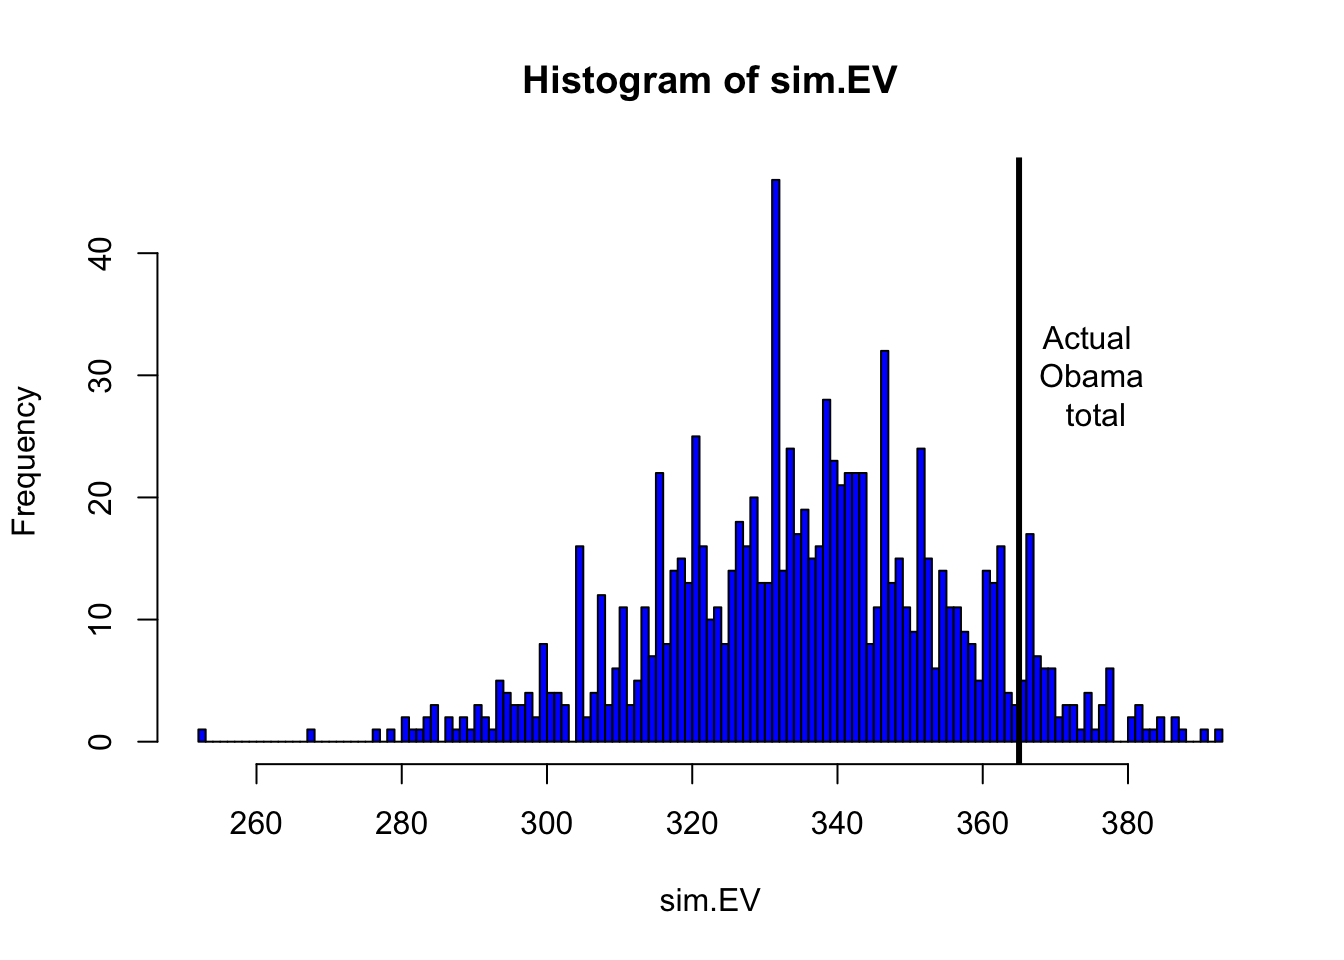
\includegraphics{bookdown-demo_files/figure-latex/unnamed-chunk-61-1.pdf}

\hypertarget{a-bioassay-experiment}{%
\section{A Bioassay Experiment}\label{a-bioassay-experiment}}

Bayesian fitting of a logistic model using data from a dose-response experiment.

\begin{Shaded}
\begin{Highlighting}[]
\NormalTok{x }\OtherTok{\textless{}{-}} \FunctionTok{c}\NormalTok{(}\SpecialCharTok{{-}}\FloatTok{0.86}\NormalTok{, }\SpecialCharTok{{-}}\FloatTok{0.3}\NormalTok{, }\SpecialCharTok{{-}}\FloatTok{0.05}\NormalTok{, }\FloatTok{0.73}\NormalTok{)}
\NormalTok{n }\OtherTok{\textless{}{-}} \FunctionTok{c}\NormalTok{(}\DecValTok{5}\NormalTok{, }\DecValTok{5}\NormalTok{, }\DecValTok{5}\NormalTok{, }\DecValTok{5}\NormalTok{)}
\NormalTok{y }\OtherTok{\textless{}{-}} \FunctionTok{c}\NormalTok{(}\DecValTok{0}\NormalTok{, }\DecValTok{1}\NormalTok{, }\DecValTok{3}\NormalTok{, }\DecValTok{5}\NormalTok{)}
\NormalTok{data }\OtherTok{\textless{}{-}} \FunctionTok{cbind}\NormalTok{(x, n, y)}
\end{Highlighting}
\end{Shaded}

Traditional logistic model fit.

\begin{Shaded}
\begin{Highlighting}[]
\NormalTok{glmdata }\OtherTok{\textless{}{-}} \FunctionTok{cbind}\NormalTok{(y, n }\SpecialCharTok{{-}}\NormalTok{ y)}
\NormalTok{results }\OtherTok{\textless{}{-}} \FunctionTok{glm}\NormalTok{(glmdata }\SpecialCharTok{\textasciitilde{}}\NormalTok{ x, }\AttributeTok{family =}\NormalTok{ binomial)}
\FunctionTok{summary}\NormalTok{(results)}
\end{Highlighting}
\end{Shaded}

\begin{verbatim}
## 
## Call:
## glm(formula = glmdata ~ x, family = binomial)
## 
## Deviance Residuals: 
##        1         2         3         4  
## -0.17236   0.08133  -0.05869   0.12237  
## 
## Coefficients:
##             Estimate Std. Error z value Pr(>|z|)
## (Intercept)   0.8466     1.0191   0.831    0.406
## x             7.7488     4.8728   1.590    0.112
## 
## (Dispersion parameter for binomial family taken to be 1)
## 
##     Null deviance: 15.791412  on 3  degrees of freedom
## Residual deviance:  0.054742  on 2  degrees of freedom
## AIC: 7.9648
## 
## Number of Fisher Scoring iterations: 7
\end{verbatim}

Illustration of a conditional means prior. When x = -.7, median and 90th percentile of p are (.2,.4). When x = +.6, median and 90th percentile of p are (.8, .95)

\begin{Shaded}
\begin{Highlighting}[]
\NormalTok{a1.b1 }\OtherTok{\textless{}{-}} \FunctionTok{beta.select}\NormalTok{(}\FunctionTok{list}\NormalTok{(}\AttributeTok{p=}\NormalTok{.}\DecValTok{5}\NormalTok{, }\AttributeTok{x=}\NormalTok{.}\DecValTok{2}\NormalTok{),}
                    \FunctionTok{list}\NormalTok{(}\AttributeTok{p=}\NormalTok{.}\DecValTok{9}\NormalTok{, }\AttributeTok{x=}\NormalTok{.}\DecValTok{5}\NormalTok{))}
\NormalTok{a2.b2 }\OtherTok{\textless{}{-}} \FunctionTok{beta.select}\NormalTok{(}\FunctionTok{list}\NormalTok{(}\AttributeTok{p=}\NormalTok{.}\DecValTok{5}\NormalTok{, }\AttributeTok{x=}\NormalTok{.}\DecValTok{8}\NormalTok{),}
                  \FunctionTok{list}\NormalTok{(}\AttributeTok{p=}\NormalTok{.}\DecValTok{9}\NormalTok{, }\AttributeTok{x=}\NormalTok{.}\DecValTok{98}\NormalTok{))}
\end{Highlighting}
\end{Shaded}

\begin{Shaded}
\begin{Highlighting}[]
\NormalTok{prior }\OtherTok{\textless{}{-}} \FunctionTok{rbind}\NormalTok{(}\FunctionTok{c}\NormalTok{(}\SpecialCharTok{{-}}\FloatTok{0.7}\NormalTok{, }\FloatTok{4.68}\NormalTok{, }\FloatTok{1.12}\NormalTok{),}
            \FunctionTok{c}\NormalTok{(}\FloatTok{0.6}\NormalTok{, }\FloatTok{2.10}\NormalTok{, }\FloatTok{0.74}\NormalTok{))}
\NormalTok{data.new }\OtherTok{\textless{}{-}} \FunctionTok{rbind}\NormalTok{(data, prior)}
\end{Highlighting}
\end{Shaded}

Plot prior.

\begin{Shaded}
\begin{Highlighting}[]
\FunctionTok{plot}\NormalTok{(}\FunctionTok{c}\NormalTok{(}\SpecialCharTok{{-}}\DecValTok{1}\NormalTok{,}\DecValTok{1}\NormalTok{), }\FunctionTok{c}\NormalTok{(}\DecValTok{0}\NormalTok{, }\DecValTok{1}\NormalTok{), }\AttributeTok{type=}\StringTok{"n"}\NormalTok{, }
     \AttributeTok{xlab=}\StringTok{"Dose"}\NormalTok{, }\AttributeTok{ylab=}\StringTok{"Prob(death)"}\NormalTok{)}
\FunctionTok{lines}\NormalTok{(}\SpecialCharTok{{-}}\FloatTok{0.7} \SpecialCharTok{*} \FunctionTok{c}\NormalTok{(}\DecValTok{1}\NormalTok{, }\DecValTok{1}\NormalTok{), }\FunctionTok{qbeta}\NormalTok{(}\FunctionTok{c}\NormalTok{(.}\DecValTok{25}\NormalTok{, .}\DecValTok{75}\NormalTok{), }
\NormalTok{      a1.b1[}\DecValTok{1}\NormalTok{], a1.b1[}\DecValTok{2}\NormalTok{]), }\AttributeTok{lwd=}\DecValTok{4}\NormalTok{)}
\FunctionTok{lines}\NormalTok{(}\FloatTok{0.6} \SpecialCharTok{*} \FunctionTok{c}\NormalTok{(}\DecValTok{1}\NormalTok{, }\DecValTok{1}\NormalTok{), }\FunctionTok{qbeta}\NormalTok{(}\FunctionTok{c}\NormalTok{(.}\DecValTok{25}\NormalTok{, .}\DecValTok{75}\NormalTok{), }
\NormalTok{      a2.b2[}\DecValTok{1}\NormalTok{], a2.b2[}\DecValTok{2}\NormalTok{]), }\AttributeTok{lwd=}\DecValTok{4}\NormalTok{)}
\FunctionTok{points}\NormalTok{(}\FunctionTok{c}\NormalTok{(}\SpecialCharTok{{-}}\FloatTok{0.7}\NormalTok{, }\FloatTok{0.6}\NormalTok{), }\FunctionTok{qbeta}\NormalTok{(.}\DecValTok{5}\NormalTok{, }\FunctionTok{c}\NormalTok{(a1.b1[}\DecValTok{1}\NormalTok{],}
\NormalTok{          a2.b2[}\DecValTok{1}\NormalTok{]), }\FunctionTok{c}\NormalTok{(a1.b1[}\DecValTok{2}\NormalTok{], a2.b2[}\DecValTok{2}\NormalTok{])),}
         \AttributeTok{pch=}\DecValTok{19}\NormalTok{, }\AttributeTok{cex=}\DecValTok{2}\NormalTok{)}
\FunctionTok{text}\NormalTok{(}\SpecialCharTok{{-}}\FloatTok{0.3}\NormalTok{, .}\DecValTok{2}\NormalTok{, }\StringTok{"Beta(1.12, 3.56)"}\NormalTok{)}
\FunctionTok{text}\NormalTok{(.}\DecValTok{2}\NormalTok{, .}\DecValTok{8}\NormalTok{, }\StringTok{"Beta(2.10, 0.74)"}\NormalTok{)}
\NormalTok{response }\OtherTok{\textless{}{-}} \FunctionTok{rbind}\NormalTok{(a1.b1, a2.b2)}
\NormalTok{x }\OtherTok{\textless{}{-}} \FunctionTok{c}\NormalTok{(}\SpecialCharTok{{-}}\FloatTok{0.7}\NormalTok{, }\FloatTok{0.6}\NormalTok{)}
\NormalTok{fit }\OtherTok{\textless{}{-}} \FunctionTok{glm}\NormalTok{(response }\SpecialCharTok{\textasciitilde{}}\NormalTok{ x, }\AttributeTok{family =}\NormalTok{ binomial)}
\end{Highlighting}
\end{Shaded}

\begin{verbatim}
## Warning in eval(family$initialize): non-integer counts in a binomial glm!
\end{verbatim}

\begin{Shaded}
\begin{Highlighting}[]
\FunctionTok{curve}\NormalTok{(}\FunctionTok{exp}\NormalTok{(fit}\SpecialCharTok{$}\NormalTok{coef[}\DecValTok{1}\NormalTok{] }\SpecialCharTok{+}\NormalTok{ fit}\SpecialCharTok{$}\NormalTok{coef[}\DecValTok{2}\NormalTok{] }\SpecialCharTok{*}\NormalTok{ x) }\SpecialCharTok{/}
\NormalTok{     (}\DecValTok{1} \SpecialCharTok{+} \FunctionTok{exp}\NormalTok{(fit}\SpecialCharTok{$}\NormalTok{coef[}\DecValTok{1}\NormalTok{] }\SpecialCharTok{+}\NormalTok{ fit}\SpecialCharTok{$}\NormalTok{coef[}\DecValTok{2}\NormalTok{] }\SpecialCharTok{*}\NormalTok{ x)),}
     \AttributeTok{add=}\NormalTok{T)}
\end{Highlighting}
\end{Shaded}

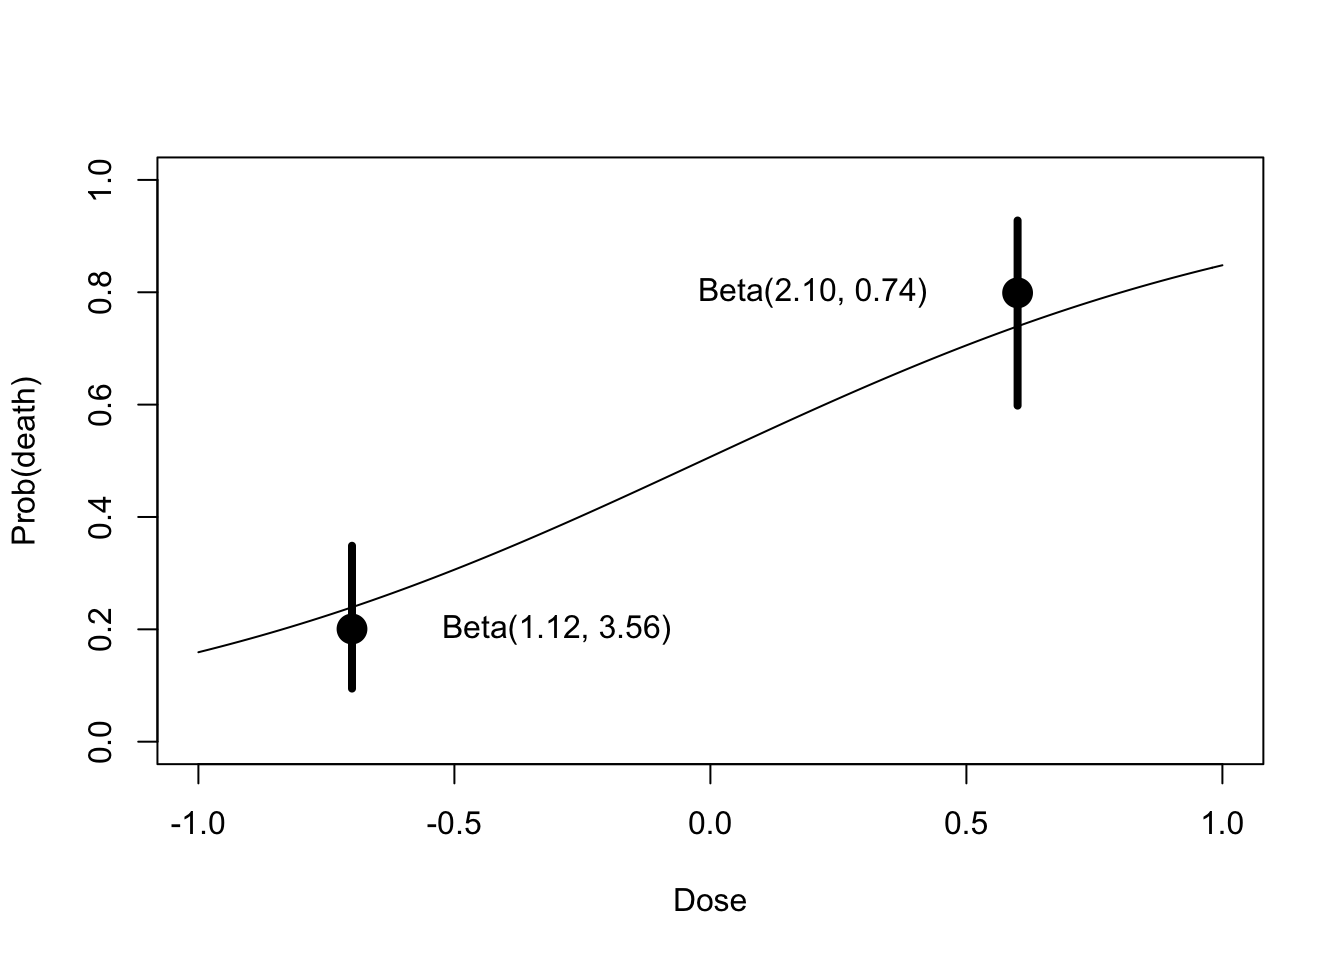
\includegraphics{bookdown-demo_files/figure-latex/unnamed-chunk-66-1.pdf}

Posterior of regression coefficients.

\begin{Shaded}
\begin{Highlighting}[]
\FunctionTok{mycontour}\NormalTok{(logisticpost, }\FunctionTok{c}\NormalTok{(}\SpecialCharTok{{-}}\DecValTok{3}\NormalTok{, }\DecValTok{3}\NormalTok{, }\SpecialCharTok{{-}}\DecValTok{1}\NormalTok{, }\DecValTok{9}\NormalTok{), data.new,}
  \AttributeTok{xlab=}\StringTok{"beta0"}\NormalTok{, }\AttributeTok{ylab=}\StringTok{"beta1"}\NormalTok{)}
\end{Highlighting}
\end{Shaded}

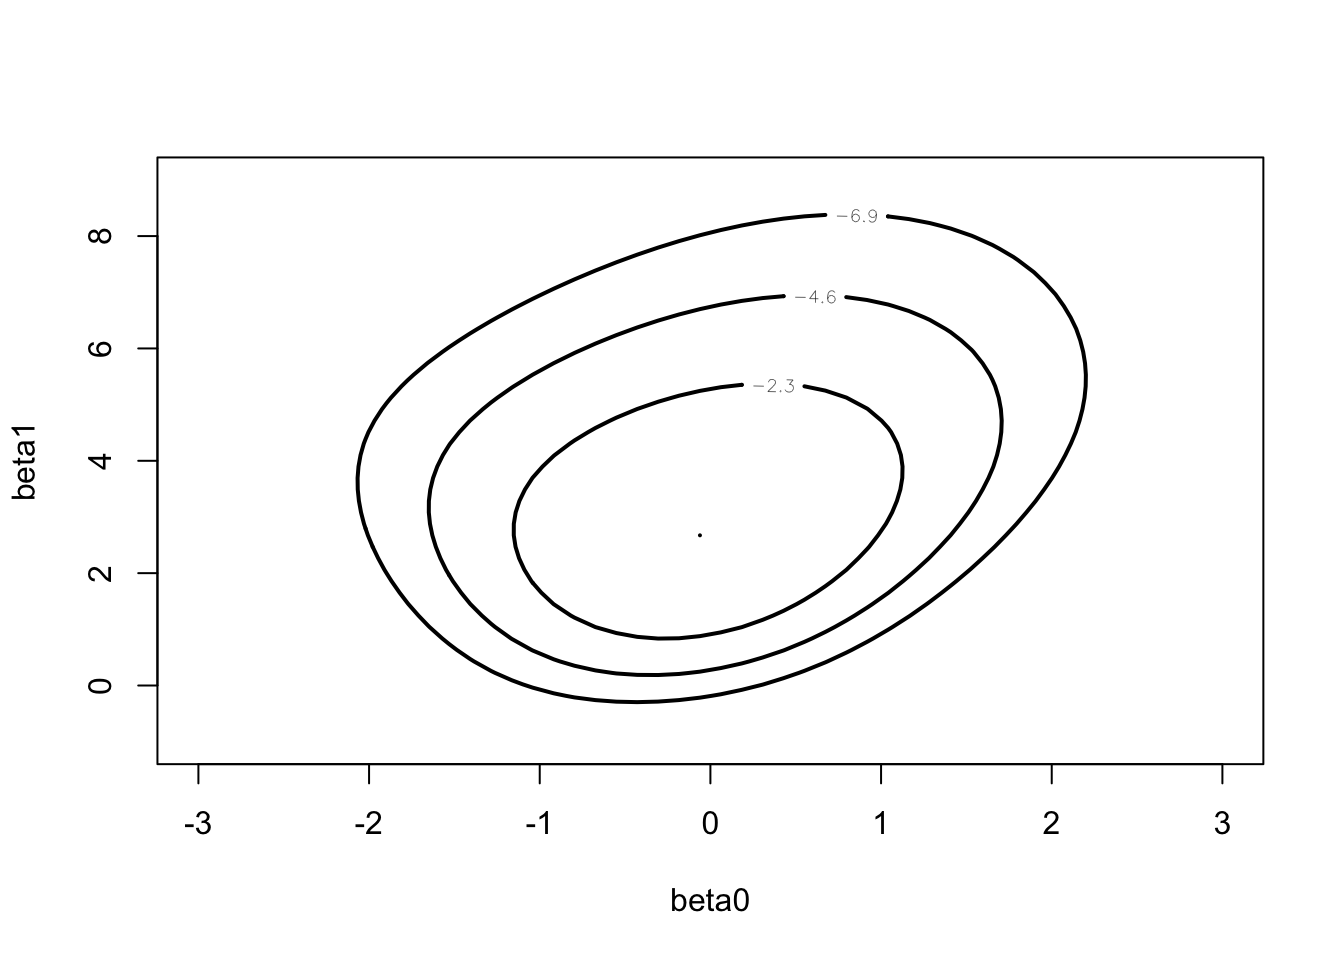
\includegraphics{bookdown-demo_files/figure-latex/unnamed-chunk-67-1.pdf}

\begin{Shaded}
\begin{Highlighting}[]
\FunctionTok{mycontour}\NormalTok{(logisticpost, }\FunctionTok{c}\NormalTok{(}\SpecialCharTok{{-}}\DecValTok{3}\NormalTok{, }\DecValTok{3}\NormalTok{, }\SpecialCharTok{{-}}\DecValTok{1}\NormalTok{, }\DecValTok{9}\NormalTok{), data.new,}
  \AttributeTok{xlab=}\StringTok{"beta0"}\NormalTok{, }\AttributeTok{ylab=}\StringTok{"beta1"}\NormalTok{)}
\NormalTok{s }\OtherTok{\textless{}{-}} \FunctionTok{simcontour}\NormalTok{(logisticpost, }\FunctionTok{c}\NormalTok{(}\SpecialCharTok{{-}}\DecValTok{2}\NormalTok{, }\DecValTok{3}\NormalTok{, }\SpecialCharTok{{-}}\DecValTok{1}\NormalTok{, }\DecValTok{11}\NormalTok{),}
\NormalTok{                data.new, }\DecValTok{1000}\NormalTok{)}
\FunctionTok{points}\NormalTok{(s)}
\end{Highlighting}
\end{Shaded}

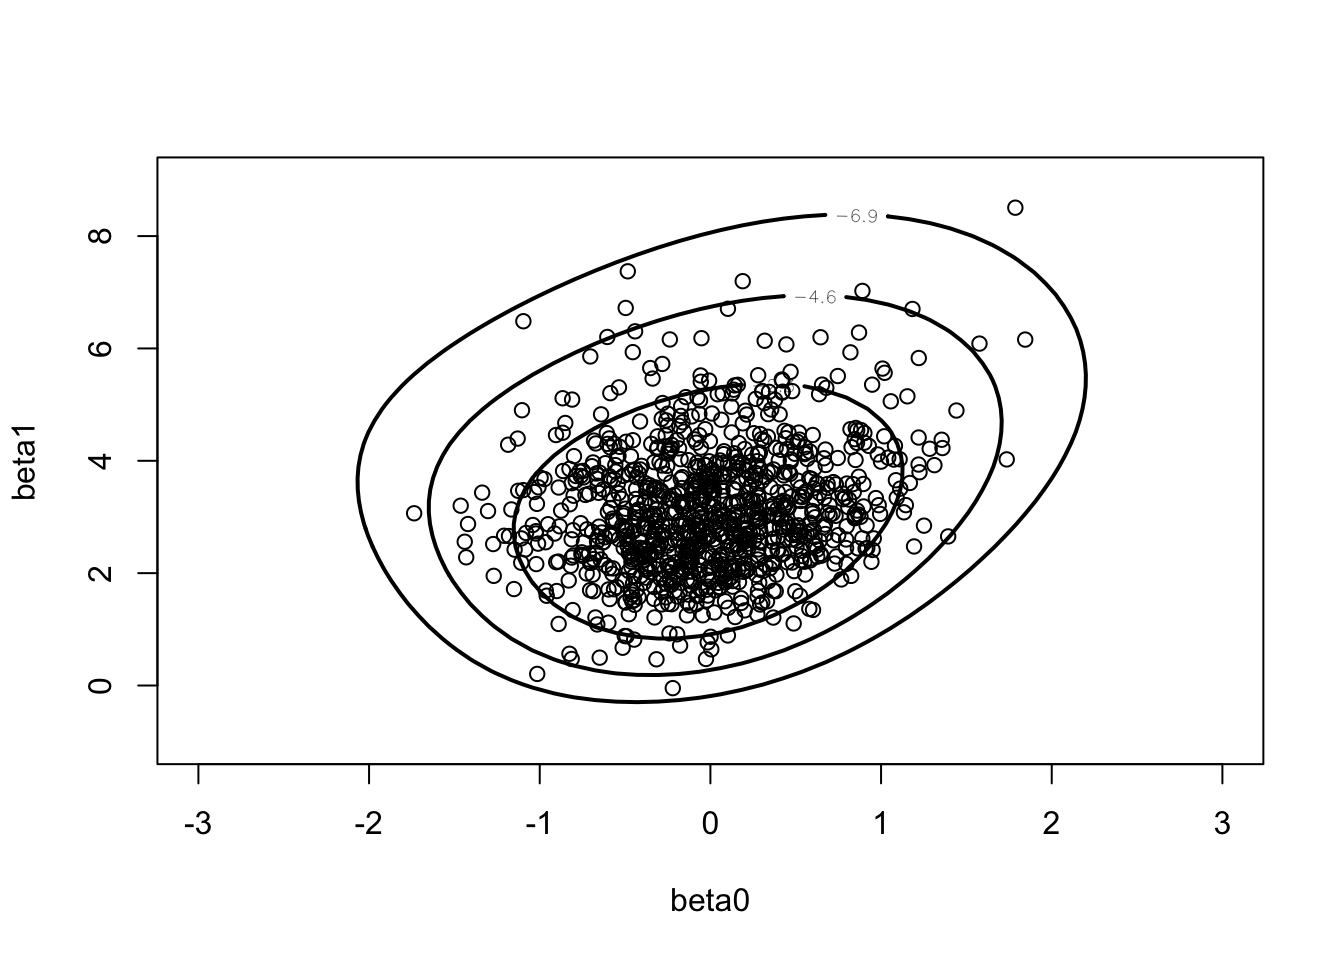
\includegraphics{bookdown-demo_files/figure-latex/unnamed-chunk-68-1.pdf}

\begin{Shaded}
\begin{Highlighting}[]
\FunctionTok{plot}\NormalTok{(}\FunctionTok{density}\NormalTok{(s}\SpecialCharTok{$}\NormalTok{y), }\AttributeTok{xlab=}\StringTok{"beta1"}\NormalTok{)}
\end{Highlighting}
\end{Shaded}

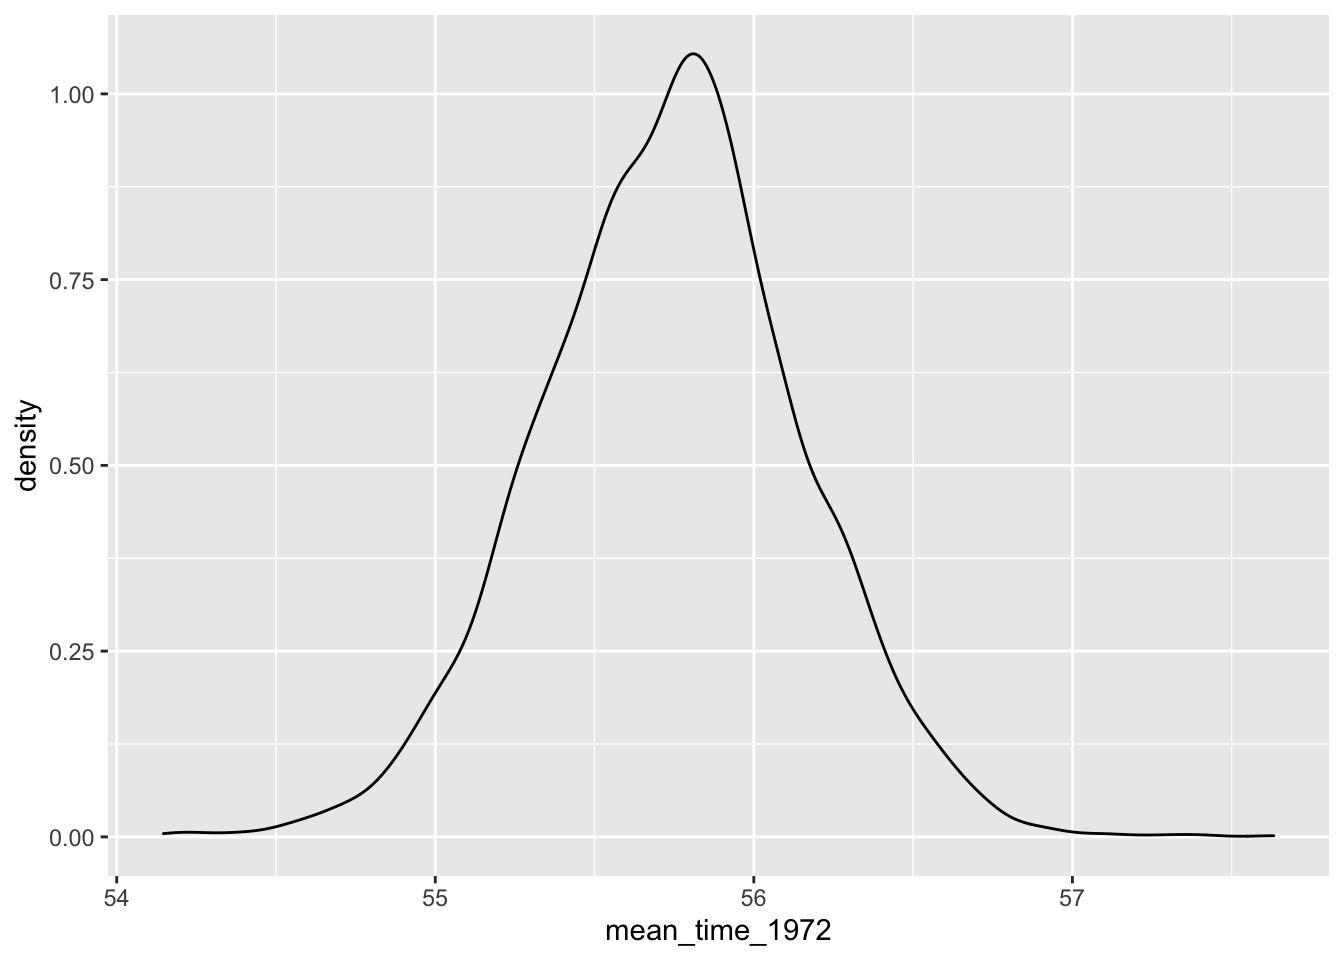
\includegraphics{bookdown-demo_files/figure-latex/unnamed-chunk-69-1.pdf}

Estimation of LD50 parameter.

\begin{Shaded}
\begin{Highlighting}[]
\NormalTok{theta }\OtherTok{\textless{}{-}} \SpecialCharTok{{-}}\NormalTok{s}\SpecialCharTok{$}\NormalTok{x }\SpecialCharTok{/}\NormalTok{ s}\SpecialCharTok{$}\NormalTok{y}
\FunctionTok{hist}\NormalTok{(theta, }\AttributeTok{xlab=}\StringTok{"LD{-}50"}\NormalTok{, }\AttributeTok{breaks=}\DecValTok{20}\NormalTok{,}
     \AttributeTok{xlim =} \FunctionTok{c}\NormalTok{(}\SpecialCharTok{{-}}\DecValTok{1}\NormalTok{, }\FloatTok{1.5}\NormalTok{))}
\end{Highlighting}
\end{Shaded}

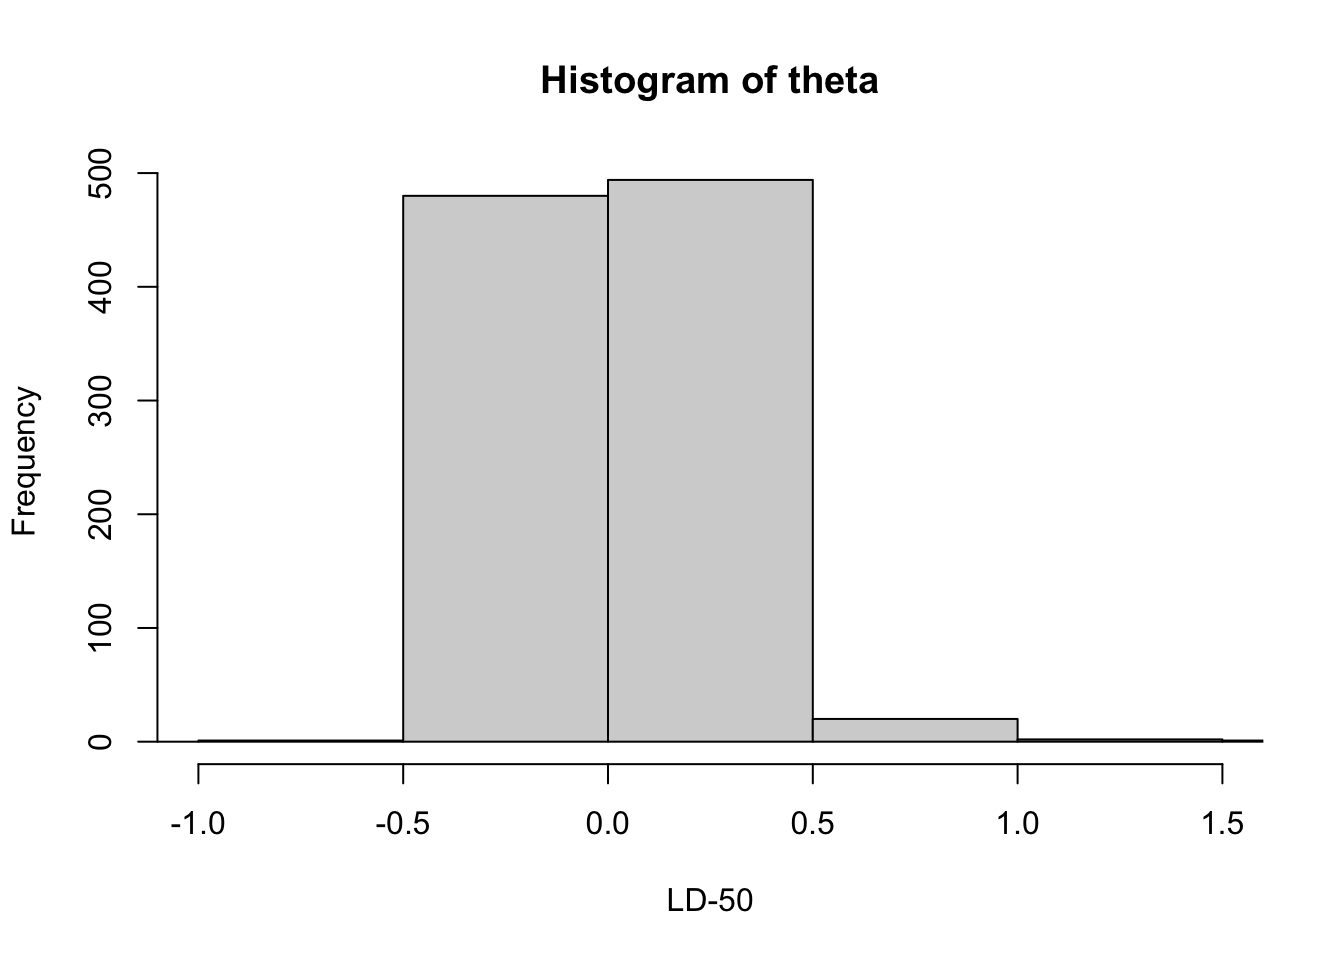
\includegraphics{bookdown-demo_files/figure-latex/unnamed-chunk-70-1.pdf}

\begin{Shaded}
\begin{Highlighting}[]
\FunctionTok{quantile}\NormalTok{(theta, }\FunctionTok{c}\NormalTok{(.}\DecValTok{025}\NormalTok{, .}\DecValTok{975}\NormalTok{))}
\end{Highlighting}
\end{Shaded}

\begin{verbatim}
##       2.5%      97.5% 
## -0.3194579  0.5101581
\end{verbatim}

\hypertarget{comparing-two-proportions}{%
\section{Comparing Two Proportions}\label{comparing-two-proportions}}

Using Howard's dependent prior for two proportions.
Graph of the prior.

\begin{Shaded}
\begin{Highlighting}[]
\NormalTok{sigma }\OtherTok{\textless{}{-}} \FunctionTok{c}\NormalTok{(}\DecValTok{2}\NormalTok{, }\DecValTok{1}\NormalTok{, .}\DecValTok{5}\NormalTok{, .}\DecValTok{25}\NormalTok{)}
\NormalTok{plo }\OtherTok{\textless{}{-}}\NormalTok{ .}\DecValTok{0001}\NormalTok{; phi }\OtherTok{\textless{}{-}}\NormalTok{ .}\DecValTok{9999}
\FunctionTok{par}\NormalTok{(}\AttributeTok{mfrow=}\FunctionTok{c}\NormalTok{(}\DecValTok{2}\NormalTok{, }\DecValTok{2}\NormalTok{))}
\ControlFlowTok{for}\NormalTok{ (i }\ControlFlowTok{in} \DecValTok{1}\SpecialCharTok{:}\DecValTok{4}\NormalTok{)\{}
    \FunctionTok{mycontour}\NormalTok{(howardprior, }
              \FunctionTok{c}\NormalTok{(plo, phi, plo, phi),}
              \FunctionTok{c}\NormalTok{(}\DecValTok{1}\NormalTok{, }\DecValTok{1}\NormalTok{, }\DecValTok{1}\NormalTok{, }\DecValTok{1}\NormalTok{, sigma[i]),}
      \AttributeTok{main=}\FunctionTok{paste}\NormalTok{(}\StringTok{"sigma="}\NormalTok{, }\FunctionTok{as.character}\NormalTok{(sigma[i])),}
      \AttributeTok{xlab=}\StringTok{"p1"}\NormalTok{, }\AttributeTok{ylab=}\StringTok{"p2"}\NormalTok{)}
\NormalTok{\}}
\end{Highlighting}
\end{Shaded}

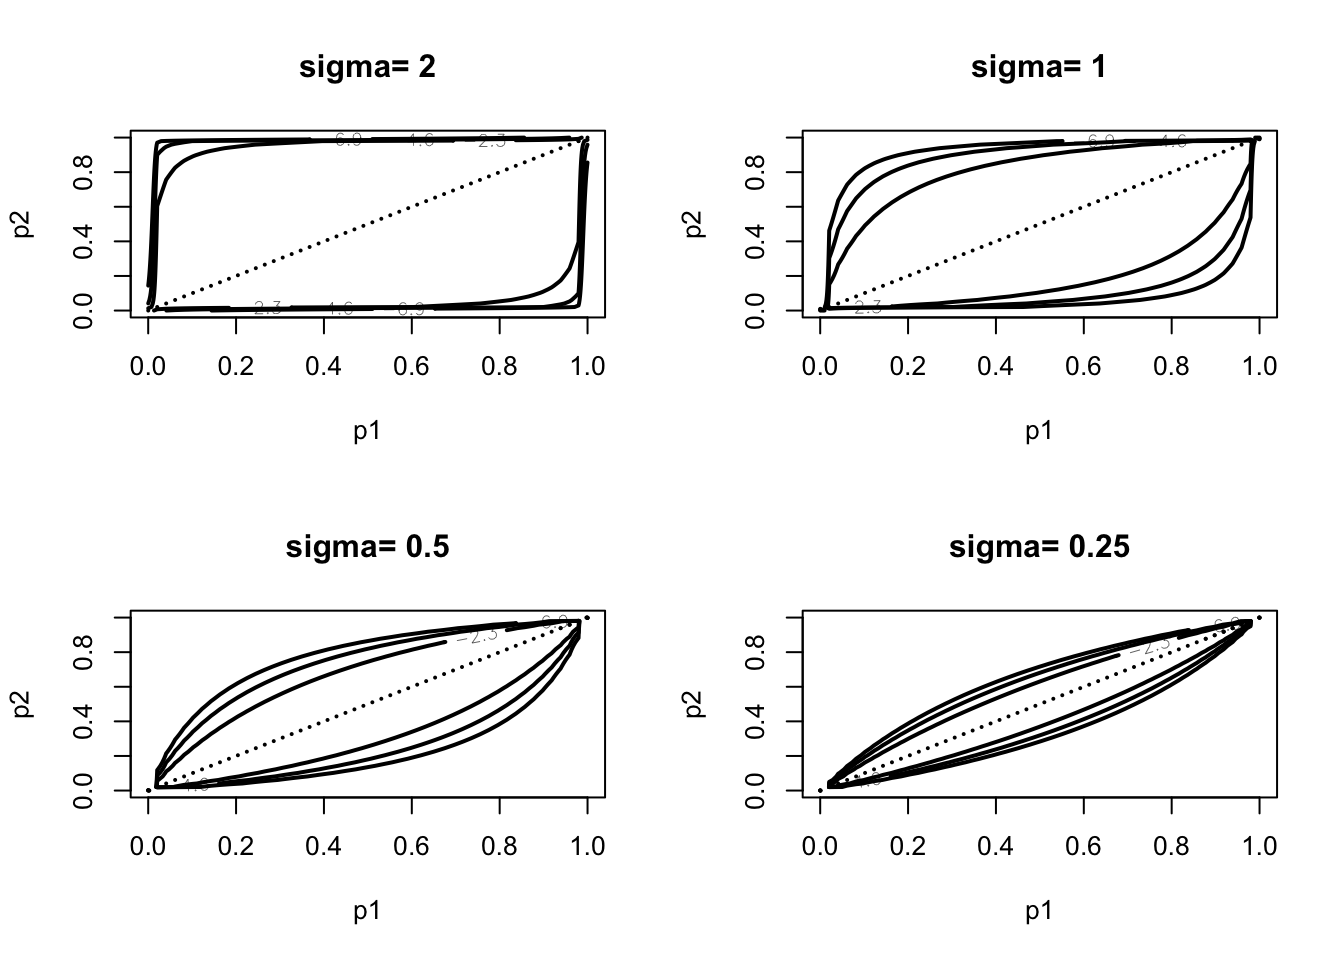
\includegraphics{bookdown-demo_files/figure-latex/unnamed-chunk-72-1.pdf}

Graphs of the posterior.

\begin{Shaded}
\begin{Highlighting}[]
\NormalTok{sigma }\OtherTok{\textless{}{-}} \FunctionTok{c}\NormalTok{(}\DecValTok{2}\NormalTok{, }\DecValTok{1}\NormalTok{, .}\DecValTok{5}\NormalTok{, .}\DecValTok{25}\NormalTok{)}
\FunctionTok{par}\NormalTok{(}\AttributeTok{mfrow=}\FunctionTok{c}\NormalTok{(}\DecValTok{2}\NormalTok{, }\DecValTok{2}\NormalTok{))}
\ControlFlowTok{for}\NormalTok{ (i }\ControlFlowTok{in} \DecValTok{1}\SpecialCharTok{:}\DecValTok{4}\NormalTok{)\{}
   \FunctionTok{mycontour}\NormalTok{(howardprior,}
             \FunctionTok{c}\NormalTok{(plo, phi, plo, phi),}
     \FunctionTok{c}\NormalTok{(}\DecValTok{1} \SpecialCharTok{+} \DecValTok{3}\NormalTok{, }\DecValTok{1} \SpecialCharTok{+} \DecValTok{15}\NormalTok{, }\DecValTok{1} \SpecialCharTok{+} \DecValTok{7}\NormalTok{, }\DecValTok{1} \SpecialCharTok{+} \DecValTok{5}\NormalTok{, sigma[i]),}
     \AttributeTok{main=}\FunctionTok{paste}\NormalTok{(}\StringTok{"sigma="}\NormalTok{, }\FunctionTok{as.character}\NormalTok{(sigma[i])),}
     \AttributeTok{xlab=}\StringTok{"p1"}\NormalTok{, }\AttributeTok{ylab=}\StringTok{"p2"}\NormalTok{)}
   \FunctionTok{lines}\NormalTok{(}\FunctionTok{c}\NormalTok{(}\DecValTok{0}\NormalTok{, }\DecValTok{1}\NormalTok{), }\FunctionTok{c}\NormalTok{(}\DecValTok{0}\NormalTok{, }\DecValTok{1}\NormalTok{))}
\NormalTok{ \}}
\end{Highlighting}
\end{Shaded}

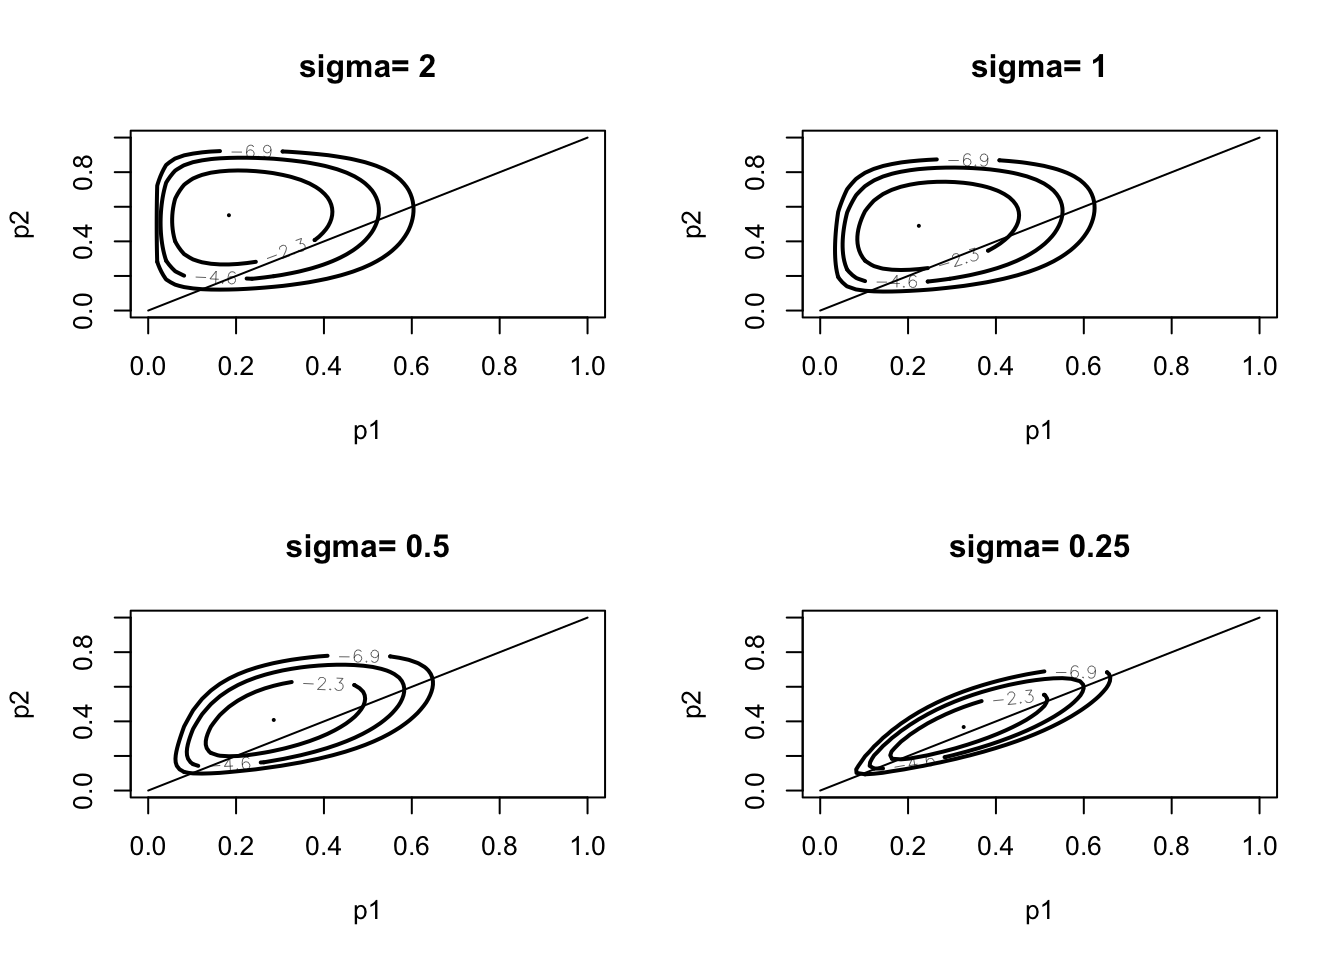
\includegraphics{bookdown-demo_files/figure-latex/unnamed-chunk-73-1.pdf}

\begin{Shaded}
\begin{Highlighting}[]
\NormalTok{s }\OtherTok{\textless{}{-}} \FunctionTok{simcontour}\NormalTok{(howardprior, }\FunctionTok{c}\NormalTok{(plo, phi, plo, phi),}
   \FunctionTok{c}\NormalTok{(}\DecValTok{1} \SpecialCharTok{+} \DecValTok{3}\NormalTok{, }\DecValTok{1} \SpecialCharTok{+} \DecValTok{15}\NormalTok{, }\DecValTok{1} \SpecialCharTok{+} \DecValTok{7}\NormalTok{, }\DecValTok{1} \SpecialCharTok{+} \DecValTok{5}\NormalTok{, }\DecValTok{2}\NormalTok{), }\DecValTok{1000}\NormalTok{)}
\FunctionTok{sum}\NormalTok{(s}\SpecialCharTok{$}\NormalTok{x }\SpecialCharTok{\textgreater{}}\NormalTok{ s}\SpecialCharTok{$}\NormalTok{y) }\SpecialCharTok{/} \DecValTok{1000}
\end{Highlighting}
\end{Shaded}

\begin{verbatim}
## [1] 0.012
\end{verbatim}

\hypertarget{introduction-to-bayesian-computation}{%
\chapter{Introduction to Bayesian Computation}\label{introduction-to-bayesian-computation}}

\hypertarget{a-beta-binomial-model-for-overdispersion}{%
\section{A Beta-Binomial Model for Overdispersion}\label{a-beta-binomial-model-for-overdispersion}}

\begin{Shaded}
\begin{Highlighting}[]
\FunctionTok{library}\NormalTok{(LearnBayes)}
\end{Highlighting}
\end{Shaded}

First consider posterior of \((\eta, K)\).

\begin{Shaded}
\begin{Highlighting}[]
\FunctionTok{mycontour}\NormalTok{(betabinexch0,}
          \FunctionTok{c}\NormalTok{(.}\DecValTok{0001}\NormalTok{, .}\DecValTok{003}\NormalTok{, }\DecValTok{1}\NormalTok{, }\DecValTok{20000}\NormalTok{),}
\NormalTok{          cancermortality,}
          \AttributeTok{xlab=}\StringTok{"eta"}\NormalTok{, }\AttributeTok{ylab=}\StringTok{"K"}\NormalTok{)}
\end{Highlighting}
\end{Shaded}

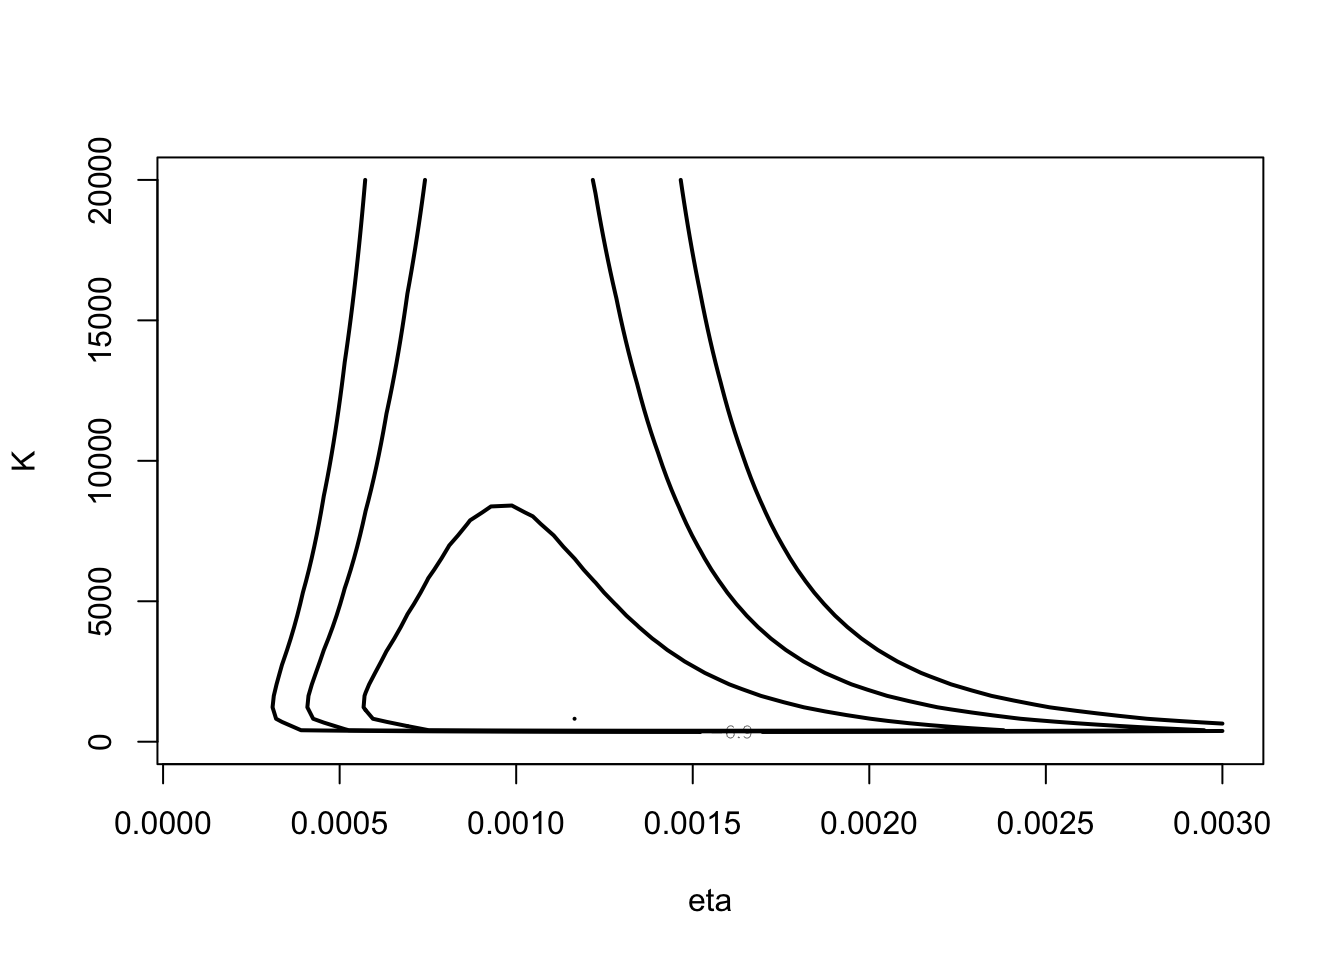
\includegraphics{bookdown-demo_files/figure-latex/unnamed-chunk-76-1.pdf}

Instead look at posterior of \((\log \frac{\eta}{1-\eta}, \log I\).

\begin{Shaded}
\begin{Highlighting}[]
\FunctionTok{mycontour}\NormalTok{(betabinexch,}
          \FunctionTok{c}\NormalTok{(}\SpecialCharTok{{-}}\DecValTok{8}\NormalTok{, }\SpecialCharTok{{-}}\FloatTok{4.5}\NormalTok{, }\DecValTok{3}\NormalTok{, }\FloatTok{16.5}\NormalTok{),}
\NormalTok{          cancermortality,}
          \AttributeTok{xlab=}\StringTok{"logit eta"}\NormalTok{, }\AttributeTok{ylab=}\StringTok{"log K"}\NormalTok{)}
\end{Highlighting}
\end{Shaded}

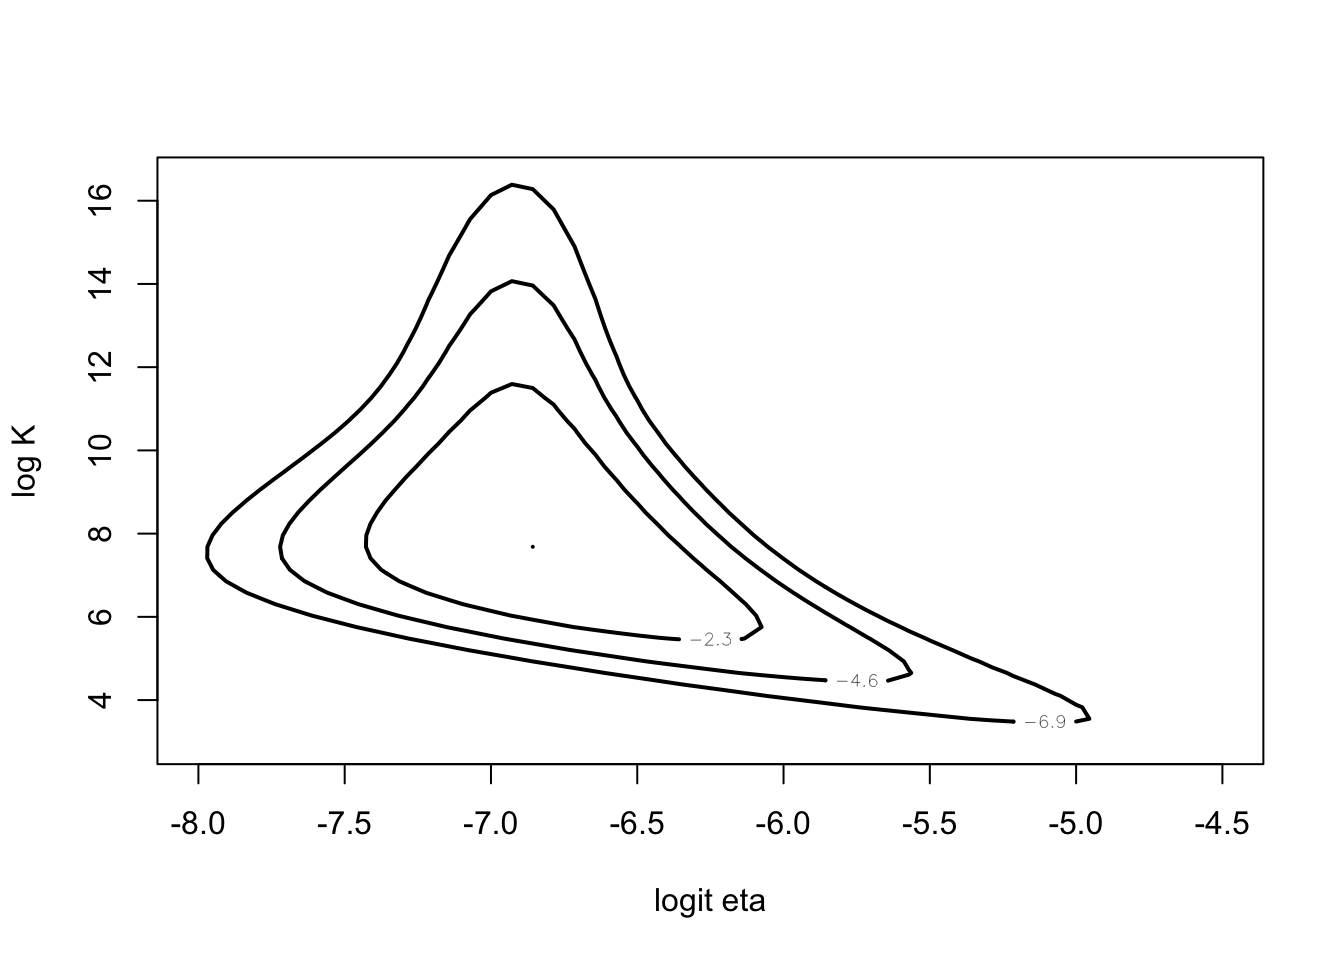
\includegraphics{bookdown-demo_files/figure-latex/unnamed-chunk-77-1.pdf}

\hypertarget{approximations-based-on-posterior-modes}{%
\section{Approximations Based on Posterior Modes}\label{approximations-based-on-posterior-modes}}

\begin{Shaded}
\begin{Highlighting}[]
\NormalTok{fit }\OtherTok{\textless{}{-}} \FunctionTok{laplace}\NormalTok{(betabinexch, }
               \FunctionTok{c}\NormalTok{(}\SpecialCharTok{{-}}\DecValTok{7}\NormalTok{, }\DecValTok{6}\NormalTok{), }
\NormalTok{               cancermortality)}
\NormalTok{fit}
\end{Highlighting}
\end{Shaded}

\begin{verbatim}
## $mode
## [1] -6.819793  7.576111
## 
## $var
##             [,1]       [,2]
## [1,]  0.07896568 -0.1485087
## [2,] -0.14850874  1.3483208
## 
## $int
## [1] -570.7743
## 
## $converge
## [1] TRUE
\end{verbatim}

\begin{Shaded}
\begin{Highlighting}[]
\NormalTok{npar }\OtherTok{\textless{}{-}} \FunctionTok{list}\NormalTok{(}\AttributeTok{m=}\NormalTok{fit}\SpecialCharTok{$}\NormalTok{mode, }\AttributeTok{v=}\NormalTok{fit}\SpecialCharTok{$}\NormalTok{var)}
\FunctionTok{mycontour}\NormalTok{(lbinorm,}
          \FunctionTok{c}\NormalTok{(}\SpecialCharTok{{-}}\DecValTok{8}\NormalTok{, }\SpecialCharTok{{-}}\FloatTok{4.5}\NormalTok{, }\DecValTok{3}\NormalTok{, }\FloatTok{16.5}\NormalTok{), }
\NormalTok{          npar,}
          \AttributeTok{xlab=}\StringTok{"logit eta"}\NormalTok{, }\AttributeTok{ylab=}\StringTok{"log K"}\NormalTok{)}
\end{Highlighting}
\end{Shaded}

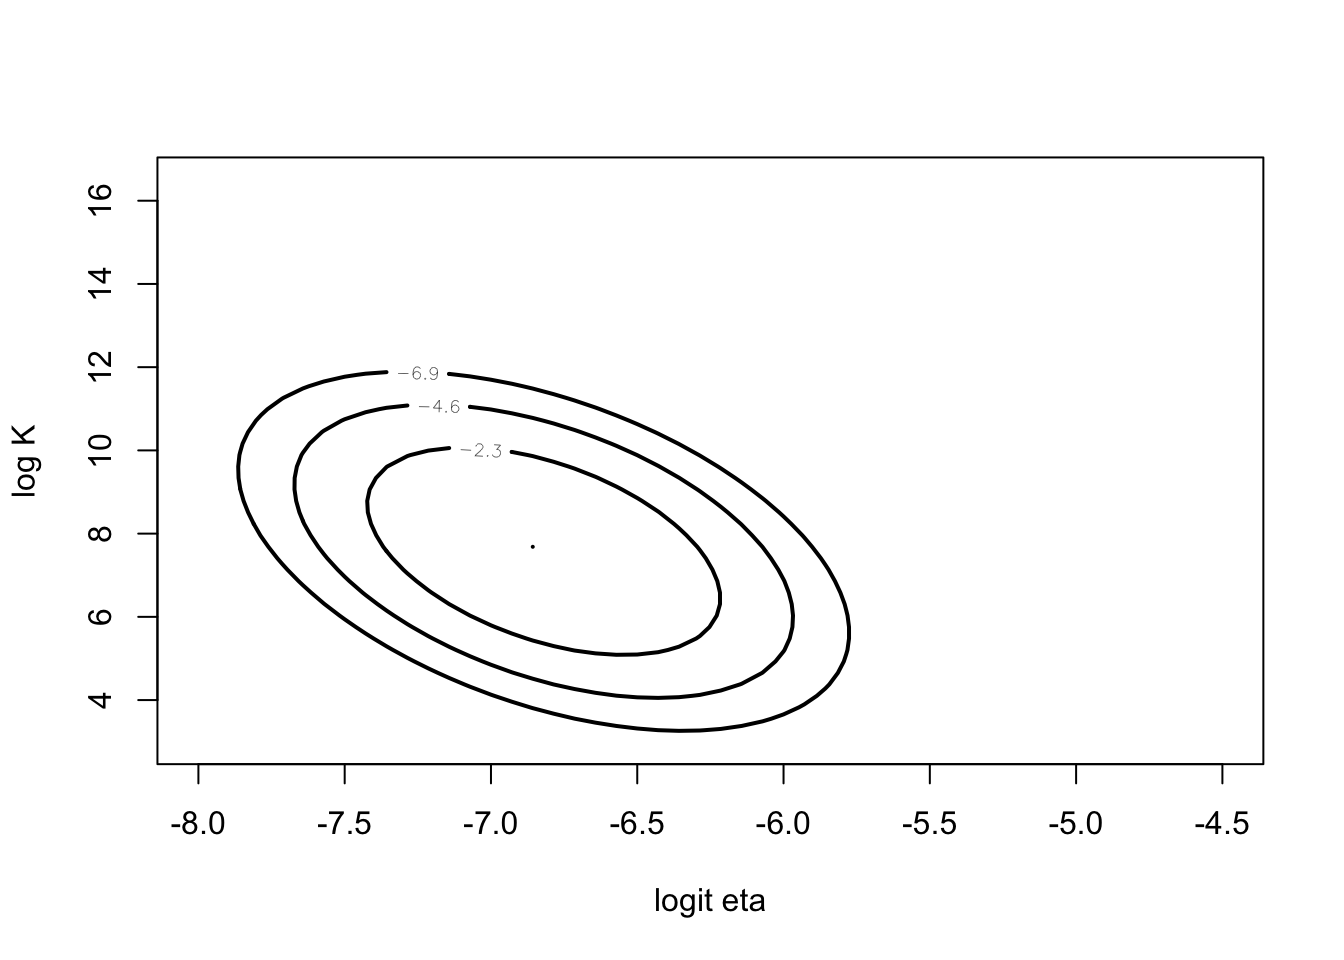
\includegraphics{bookdown-demo_files/figure-latex/unnamed-chunk-79-1.pdf}

\begin{Shaded}
\begin{Highlighting}[]
\NormalTok{se }\OtherTok{\textless{}{-}} \FunctionTok{sqrt}\NormalTok{(}\FunctionTok{diag}\NormalTok{(fit}\SpecialCharTok{$}\NormalTok{var))}
\NormalTok{fit}\SpecialCharTok{$}\NormalTok{mode }\SpecialCharTok{{-}} \FloatTok{1.645} \SpecialCharTok{*}\NormalTok{ se}
\end{Highlighting}
\end{Shaded}

\begin{verbatim}
## [1] -7.282052  5.665982
\end{verbatim}

\begin{Shaded}
\begin{Highlighting}[]
\NormalTok{fit}\SpecialCharTok{$}\NormalTok{mode }\SpecialCharTok{+} \FloatTok{1.645} \SpecialCharTok{*}\NormalTok{ se}
\end{Highlighting}
\end{Shaded}

\begin{verbatim}
## [1] -6.357535  9.486239
\end{verbatim}

\hypertarget{monte-carlo-method-for-computing-integrals}{%
\section{Monte Carlo Method for Computing Integrals}\label{monte-carlo-method-for-computing-integrals}}

Illustration of a simple estimate of an integral by Monte Carlo.

\begin{Shaded}
\begin{Highlighting}[]
\NormalTok{p }\OtherTok{\textless{}{-}} \FunctionTok{rbeta}\NormalTok{(}\DecValTok{1000}\NormalTok{, }\FloatTok{14.26}\NormalTok{, }\FloatTok{23.19}\NormalTok{)}
\NormalTok{est }\OtherTok{\textless{}{-}} \FunctionTok{mean}\NormalTok{(p }\SpecialCharTok{\^{}} \DecValTok{2}\NormalTok{)}
\NormalTok{se }\OtherTok{\textless{}{-}} \FunctionTok{sd}\NormalTok{(p }\SpecialCharTok{\^{}} \DecValTok{2}\NormalTok{) }\SpecialCharTok{/} \FunctionTok{sqrt}\NormalTok{(}\DecValTok{1000}\NormalTok{)}
\FunctionTok{c}\NormalTok{(est,se)}
\end{Highlighting}
\end{Shaded}

\begin{verbatim}
## [1] 0.151521812 0.001944763
\end{verbatim}

\hypertarget{rejection-sampling}{%
\section{Rejection Sampling}\label{rejection-sampling}}

Using rejection sampling for the overdispersion posterior with a multivariate t proposal density.

\begin{Shaded}
\begin{Highlighting}[]
\NormalTok{fit }\OtherTok{\textless{}{-}} \FunctionTok{laplace}\NormalTok{(betabinexch,}
               \FunctionTok{c}\NormalTok{(}\SpecialCharTok{{-}}\DecValTok{7}\NormalTok{, }\DecValTok{6}\NormalTok{),}
\NormalTok{               cancermortality)}
\end{Highlighting}
\end{Shaded}

\begin{Shaded}
\begin{Highlighting}[]
\NormalTok{betabinT }\OtherTok{\textless{}{-}} \ControlFlowTok{function}\NormalTok{(theta, datapar)\{}
\NormalTok{  data }\OtherTok{\textless{}{-}}\NormalTok{ datapar}\SpecialCharTok{$}\NormalTok{data}
\NormalTok{  tpar }\OtherTok{\textless{}{-}}\NormalTok{datapar}\SpecialCharTok{$}\NormalTok{par}
\NormalTok{  d }\OtherTok{\textless{}{-}} \FunctionTok{betabinexch}\NormalTok{(theta,data) }\SpecialCharTok{{-}}
         \FunctionTok{dmt}\NormalTok{(theta, }\AttributeTok{mean=}\FunctionTok{c}\NormalTok{(tpar}\SpecialCharTok{$}\NormalTok{m),}
             \AttributeTok{S=}\NormalTok{tpar}\SpecialCharTok{$}\NormalTok{var, }\AttributeTok{df=}\NormalTok{tpar}\SpecialCharTok{$}\NormalTok{df, }\AttributeTok{log=}\ConstantTok{TRUE}\NormalTok{)}
\NormalTok{  d}
\NormalTok{\}}
\end{Highlighting}
\end{Shaded}

\begin{Shaded}
\begin{Highlighting}[]
\NormalTok{tpar }\OtherTok{\textless{}{-}} \FunctionTok{list}\NormalTok{(}\AttributeTok{m=}\NormalTok{fit}\SpecialCharTok{$}\NormalTok{mode, }\AttributeTok{var=}\DecValTok{2} \SpecialCharTok{*}\NormalTok{ fit}\SpecialCharTok{$}\NormalTok{var, }\AttributeTok{df=}\DecValTok{4}\NormalTok{)}
\NormalTok{datapar }\OtherTok{\textless{}{-}} \FunctionTok{list}\NormalTok{(}\AttributeTok{data=}\NormalTok{cancermortality, }\AttributeTok{par=}\NormalTok{tpar)}
\end{Highlighting}
\end{Shaded}

\begin{Shaded}
\begin{Highlighting}[]
\NormalTok{start }\OtherTok{\textless{}{-}} \FunctionTok{c}\NormalTok{(}\SpecialCharTok{{-}}\FloatTok{6.9}\NormalTok{, }\FloatTok{12.4}\NormalTok{)}
\NormalTok{fit1 }\OtherTok{\textless{}{-}} \FunctionTok{laplace}\NormalTok{(betabinT, start, datapar)}
\NormalTok{fit1}\SpecialCharTok{$}\NormalTok{mode}
\end{Highlighting}
\end{Shaded}

\begin{verbatim}
## [1] -6.888963 12.421993
\end{verbatim}

\begin{Shaded}
\begin{Highlighting}[]
\FunctionTok{betabinT}\NormalTok{(fit1}\SpecialCharTok{$}\NormalTok{mode, datapar)}
\end{Highlighting}
\end{Shaded}

\begin{verbatim}
## [1] -569.2829
\end{verbatim}

\begin{Shaded}
\begin{Highlighting}[]
\NormalTok{theta }\OtherTok{\textless{}{-}} \FunctionTok{rejectsampling}\NormalTok{(betabinexch,}
\NormalTok{                        tpar,}
                      \SpecialCharTok{{-}}\FloatTok{569.2813}\NormalTok{, }
                      \DecValTok{10000}\NormalTok{,}
\NormalTok{                      cancermortality)}
\FunctionTok{dim}\NormalTok{(theta)}
\end{Highlighting}
\end{Shaded}

\begin{verbatim}
## [1] 2389    2
\end{verbatim}

\begin{Shaded}
\begin{Highlighting}[]
\FunctionTok{mycontour}\NormalTok{(betabinexch, }
          \FunctionTok{c}\NormalTok{(}\SpecialCharTok{{-}}\DecValTok{8}\NormalTok{, }\SpecialCharTok{{-}}\FloatTok{4.5}\NormalTok{, }\DecValTok{3}\NormalTok{, }\FloatTok{16.5}\NormalTok{), }
\NormalTok{          cancermortality,}
          \AttributeTok{xlab=}\StringTok{"logit eta"}\NormalTok{, }\AttributeTok{ylab=}\StringTok{"log K"}\NormalTok{)}
\FunctionTok{points}\NormalTok{(theta[,}\DecValTok{1}\NormalTok{],theta[,}\DecValTok{2}\NormalTok{])}
\end{Highlighting}
\end{Shaded}

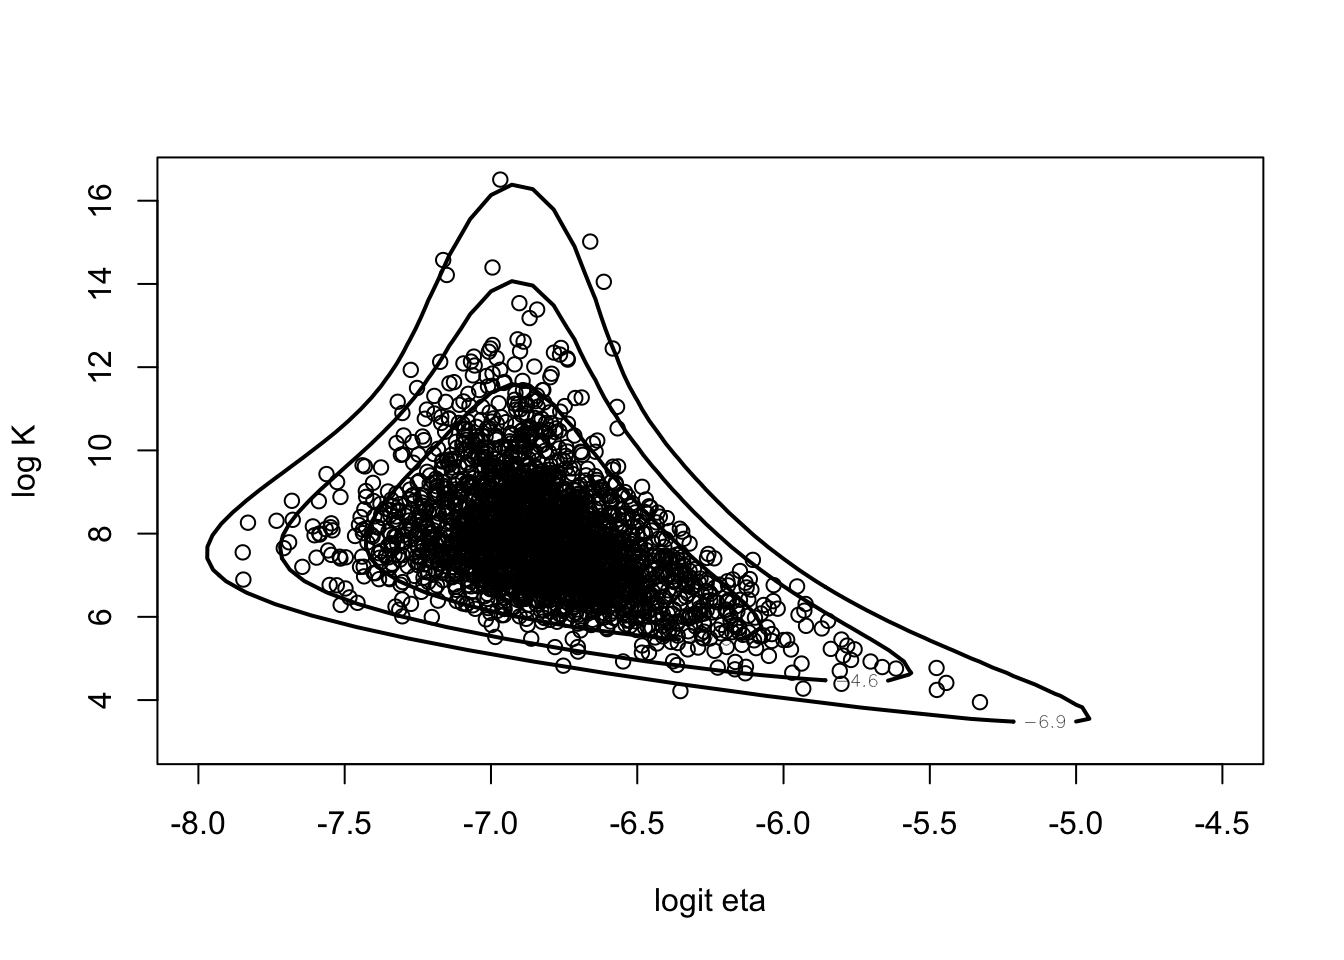
\includegraphics{bookdown-demo_files/figure-latex/unnamed-chunk-88-1.pdf}

\hypertarget{importance-sampling}{%
\section{Importance Sampling}\label{importance-sampling}}

\begin{Shaded}
\begin{Highlighting}[]
\NormalTok{fit }\OtherTok{\textless{}{-}} \FunctionTok{laplace}\NormalTok{(betabinexch,}
               \FunctionTok{c}\NormalTok{(}\SpecialCharTok{{-}}\DecValTok{7}\NormalTok{, }\DecValTok{6}\NormalTok{),}
\NormalTok{               cancermortality)}
\end{Highlighting}
\end{Shaded}

Posterior density of \(\log K\)\$ conditional on a value of \(\eta\).

\begin{Shaded}
\begin{Highlighting}[]
\NormalTok{betabinexch.cond }\OtherTok{\textless{}{-}} \ControlFlowTok{function}\NormalTok{ (log.K, data)\{}
\NormalTok{  eta }\OtherTok{\textless{}{-}} \FunctionTok{exp}\NormalTok{(}\SpecialCharTok{{-}}\FloatTok{6.818793}\NormalTok{) }\SpecialCharTok{/}\NormalTok{ (}\DecValTok{1} \SpecialCharTok{+} \FunctionTok{exp}\NormalTok{(}\SpecialCharTok{{-}}\FloatTok{6.818793}\NormalTok{))}
\NormalTok{  K }\OtherTok{\textless{}{-}} \FunctionTok{exp}\NormalTok{(log.K)}
\NormalTok{  y }\OtherTok{\textless{}{-}}\NormalTok{ data[, }\DecValTok{1}\NormalTok{]}
\NormalTok{  n }\OtherTok{\textless{}{-}}\NormalTok{ data[, }\DecValTok{2}\NormalTok{]}
\NormalTok{  N }\OtherTok{\textless{}{-}} \FunctionTok{length}\NormalTok{(y)}
\NormalTok{  logf }\OtherTok{\textless{}{-}} \DecValTok{0} \SpecialCharTok{*}\NormalTok{ log.K}
  \ControlFlowTok{for}\NormalTok{ (j }\ControlFlowTok{in} \DecValTok{1}\SpecialCharTok{:}\FunctionTok{length}\NormalTok{(y))\{}
\NormalTok{     logf }\OtherTok{=}\NormalTok{ logf }\SpecialCharTok{+} \FunctionTok{lbeta}\NormalTok{(K }\SpecialCharTok{*}\NormalTok{ eta }\SpecialCharTok{+}\NormalTok{ y[j], }
\NormalTok{                 K }\SpecialCharTok{*}\NormalTok{ (}\DecValTok{1} \SpecialCharTok{{-}}\NormalTok{ eta) }\SpecialCharTok{+}\NormalTok{ n[j] }\SpecialCharTok{{-}}\NormalTok{ y[j]) }\SpecialCharTok{{-}}
                \FunctionTok{lbeta}\NormalTok{(K }\SpecialCharTok{*}\NormalTok{ eta, K }\SpecialCharTok{*}\NormalTok{ (}\DecValTok{1} \SpecialCharTok{{-}}\NormalTok{ eta))}
\NormalTok{  \}}
\NormalTok{  val }\OtherTok{\textless{}{-}}\NormalTok{ logf }\SpecialCharTok{+}\NormalTok{ log.K }\SpecialCharTok{{-}} \DecValTok{2} \SpecialCharTok{*} \FunctionTok{log}\NormalTok{(}\DecValTok{1} \SpecialCharTok{+}\NormalTok{ K)}
  \FunctionTok{exp}\NormalTok{(val}\SpecialCharTok{{-}}\FunctionTok{max}\NormalTok{(val))}
\NormalTok{\}}
\end{Highlighting}
\end{Shaded}

Illustrate different choices of importance sampler.

\begin{Shaded}
\begin{Highlighting}[]
\NormalTok{I }\OtherTok{\textless{}{-}} \FunctionTok{integrate}\NormalTok{(betabinexch.cond, }\DecValTok{2}\NormalTok{, }\DecValTok{16}\NormalTok{,}
\NormalTok{               cancermortality)}
\FunctionTok{par}\NormalTok{(}\AttributeTok{mfrow=}\FunctionTok{c}\NormalTok{(}\DecValTok{2}\NormalTok{, }\DecValTok{2}\NormalTok{))}
\FunctionTok{curve}\NormalTok{(}\FunctionTok{betabinexch.cond}\NormalTok{(x, }
\NormalTok{            cancermortality) }\SpecialCharTok{/}\NormalTok{ I}\SpecialCharTok{$}\NormalTok{value, }
            \AttributeTok{from=}\DecValTok{3}\NormalTok{, }\AttributeTok{to=}\DecValTok{16}\NormalTok{,}
            \AttributeTok{ylab=}\StringTok{"Density"}\NormalTok{, }\AttributeTok{xlab=}\StringTok{"log K"}\NormalTok{, }\AttributeTok{lwd=}\DecValTok{3}\NormalTok{,              }\AttributeTok{main=}\StringTok{"Densities"}\NormalTok{)}
\FunctionTok{curve}\NormalTok{(}\FunctionTok{dnorm}\NormalTok{(x, }\DecValTok{8}\NormalTok{, }\DecValTok{2}\NormalTok{), }\AttributeTok{add=}\ConstantTok{TRUE}\NormalTok{)}
\FunctionTok{legend}\NormalTok{(}\StringTok{"topright"}\NormalTok{,}
       \AttributeTok{legend=}\FunctionTok{c}\NormalTok{(}\StringTok{"Exact"}\NormalTok{, }\StringTok{"Normal"}\NormalTok{),}
       \AttributeTok{lwd=}\FunctionTok{c}\NormalTok{(}\DecValTok{3}\NormalTok{, }\DecValTok{1}\NormalTok{))}
\FunctionTok{curve}\NormalTok{(}\FunctionTok{betabinexch.cond}\NormalTok{(x,}
\NormalTok{            cancermortality) }\SpecialCharTok{/}\NormalTok{ I}\SpecialCharTok{$}\NormalTok{value }\SpecialCharTok{/}
           \FunctionTok{dnorm}\NormalTok{(x, }\DecValTok{8}\NormalTok{, }\DecValTok{2}\NormalTok{), }\AttributeTok{from=}\DecValTok{3}\NormalTok{, }\AttributeTok{to=}\DecValTok{16}\NormalTok{,                 }\AttributeTok{ylab=}\StringTok{"Weight"}\NormalTok{, }\AttributeTok{xlab=}\StringTok{"log K"}\NormalTok{,}
       \AttributeTok{main=}\StringTok{"Weight = g/p"}\NormalTok{)}
\FunctionTok{curve}\NormalTok{(}\FunctionTok{betabinexch.cond}\NormalTok{(x, }
\NormalTok{            cancermortality) }\SpecialCharTok{/}\NormalTok{I}\SpecialCharTok{$}\NormalTok{value, }
          \AttributeTok{from=}\DecValTok{3}\NormalTok{, }\AttributeTok{to=}\DecValTok{16}\NormalTok{,}
          \AttributeTok{ylab=}\StringTok{"Density"}\NormalTok{, }\AttributeTok{xlab=}\StringTok{"log K"}\NormalTok{, }
          \AttributeTok{lwd=}\DecValTok{3}\NormalTok{, }\AttributeTok{main=}\StringTok{"Densities"}\NormalTok{)}
\FunctionTok{curve}\NormalTok{(}\DecValTok{1} \SpecialCharTok{/} \DecValTok{2} \SpecialCharTok{*} \FunctionTok{dt}\NormalTok{(x }\SpecialCharTok{{-}} \DecValTok{8}\NormalTok{, }\AttributeTok{df=}\DecValTok{2}\NormalTok{), }\AttributeTok{add=}\ConstantTok{TRUE}\NormalTok{)}
\FunctionTok{legend}\NormalTok{(}\StringTok{"topright"}\NormalTok{, }\AttributeTok{legend=}\FunctionTok{c}\NormalTok{(}\StringTok{"Exact"}\NormalTok{, }\StringTok{"T(2)"}\NormalTok{), }\AttributeTok{lwd=}\FunctionTok{c}\NormalTok{(}\DecValTok{3}\NormalTok{, }\DecValTok{1}\NormalTok{))}
\FunctionTok{curve}\NormalTok{(}\FunctionTok{betabinexch.cond}\NormalTok{(x, }
\NormalTok{          cancermortality) }\SpecialCharTok{/}\NormalTok{ I}\SpecialCharTok{$}\NormalTok{value }\SpecialCharTok{/}
\NormalTok{        (}\DecValTok{1} \SpecialCharTok{/} \DecValTok{2} \SpecialCharTok{*} \FunctionTok{dt}\NormalTok{(x }\SpecialCharTok{{-}} \DecValTok{8}\NormalTok{, }\AttributeTok{df=}\DecValTok{2}\NormalTok{)), }
        \AttributeTok{from=}\DecValTok{3}\NormalTok{, }\AttributeTok{to=}\DecValTok{16}\NormalTok{, }
        \AttributeTok{ylab=}\StringTok{"Weight"}\NormalTok{, }\AttributeTok{xlab=}\StringTok{"log K"}\NormalTok{,}
        \AttributeTok{main=}\StringTok{"Weight = g/p"}\NormalTok{)}
\end{Highlighting}
\end{Shaded}

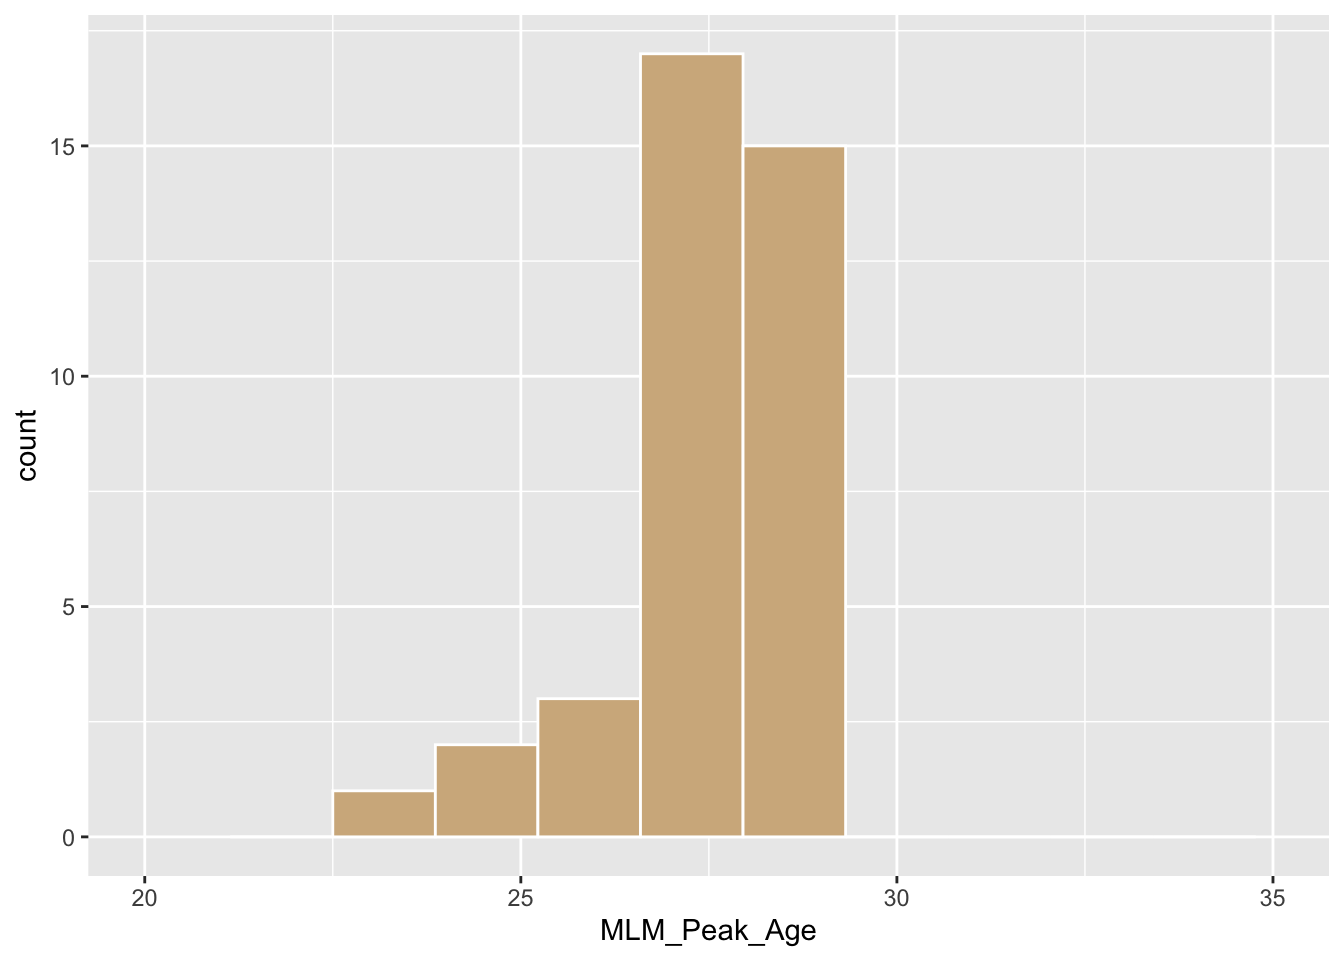
\includegraphics{bookdown-demo_files/figure-latex/unnamed-chunk-91-1.pdf}

\begin{Shaded}
\begin{Highlighting}[]
\NormalTok{tpar }\OtherTok{\textless{}{-}} \FunctionTok{list}\NormalTok{(}\AttributeTok{m=}\NormalTok{fit}\SpecialCharTok{$}\NormalTok{mode,}
             \AttributeTok{var=}\DecValTok{2} \SpecialCharTok{*}\NormalTok{ fit}\SpecialCharTok{$}\NormalTok{var, }
             \AttributeTok{df=}\DecValTok{4}\NormalTok{)}
\NormalTok{myfunc }\OtherTok{\textless{}{-}} \ControlFlowTok{function}\NormalTok{(theta)\{}
   \FunctionTok{return}\NormalTok{(theta[}\DecValTok{2}\NormalTok{])}
\NormalTok{\}}
\NormalTok{s }\OtherTok{\textless{}{-}} \FunctionTok{impsampling}\NormalTok{(betabinexch,}
\NormalTok{                 tpar,}
\NormalTok{                 myfunc,}
                 \DecValTok{10000}\NormalTok{,}
\NormalTok{                 cancermortality)}
\FunctionTok{cbind}\NormalTok{(s}\SpecialCharTok{$}\NormalTok{est, s}\SpecialCharTok{$}\NormalTok{se)}
\end{Highlighting}
\end{Shaded}

\begin{verbatim}
##          [,1]       [,2]
## [1,] 7.965118 0.01952959
\end{verbatim}

\hypertarget{sampling-importance-resampling}{%
\section{Sampling Importance Resampling}\label{sampling-importance-resampling}}

Illustrate using the SIR algorithm for the beta-binomial density with a multivariate t proposal density.

\begin{Shaded}
\begin{Highlighting}[]
\NormalTok{fit }\OtherTok{\textless{}{-}} \FunctionTok{laplace}\NormalTok{(betabinexch, }
               \FunctionTok{c}\NormalTok{(}\SpecialCharTok{{-}}\DecValTok{7}\NormalTok{, }\DecValTok{6}\NormalTok{), }
\NormalTok{               cancermortality)}
\end{Highlighting}
\end{Shaded}

\begin{Shaded}
\begin{Highlighting}[]
\NormalTok{tpar }\OtherTok{\textless{}{-}} \FunctionTok{list}\NormalTok{(}\AttributeTok{m=}\NormalTok{fit}\SpecialCharTok{$}\NormalTok{mode,}
             \AttributeTok{var=}\DecValTok{2} \SpecialCharTok{*}\NormalTok{ fit}\SpecialCharTok{$}\NormalTok{var, }\AttributeTok{df=}\DecValTok{4}\NormalTok{)}
\end{Highlighting}
\end{Shaded}

\begin{Shaded}
\begin{Highlighting}[]
\NormalTok{theta.s }\OtherTok{\textless{}{-}} \FunctionTok{sir}\NormalTok{(betabinexch, }
\NormalTok{               tpar, }\DecValTok{10000}\NormalTok{, }
\NormalTok{               cancermortality)}
\end{Highlighting}
\end{Shaded}

Use SIR to examine the sensitivity of the posterior inference to removal of individual observations.

\begin{Shaded}
\begin{Highlighting}[]
\NormalTok{S }\OtherTok{\textless{}{-}} \FunctionTok{bayes.influence}\NormalTok{(theta.s, cancermortality)}
\FunctionTok{plot}\NormalTok{(}\FunctionTok{c}\NormalTok{(}\DecValTok{0}\NormalTok{, }\DecValTok{0}\NormalTok{, }\DecValTok{0}\NormalTok{), S}\SpecialCharTok{$}\NormalTok{summary, }
     \AttributeTok{type=}\StringTok{"b"}\NormalTok{, }\AttributeTok{lwd=}\DecValTok{3}\NormalTok{, }\AttributeTok{xlim=}\FunctionTok{c}\NormalTok{(}\SpecialCharTok{{-}}\DecValTok{1}\NormalTok{, }\DecValTok{21}\NormalTok{),}
     \AttributeTok{ylim=}\FunctionTok{c}\NormalTok{(}\DecValTok{5}\NormalTok{, }\DecValTok{11}\NormalTok{), }
     \AttributeTok{xlab=}\StringTok{"Observation removed"}\NormalTok{,  }\AttributeTok{ylab=}\StringTok{"log K"}\NormalTok{)}
\ControlFlowTok{for}\NormalTok{ (i }\ControlFlowTok{in} \DecValTok{1}\SpecialCharTok{:}\DecValTok{20}\NormalTok{)\{}
  \FunctionTok{lines}\NormalTok{(}\FunctionTok{c}\NormalTok{(i, i, i), S}\SpecialCharTok{$}\NormalTok{summary.obs[i, ], }\AttributeTok{type=}\StringTok{"b"}\NormalTok{)}
\NormalTok{\}}
\end{Highlighting}
\end{Shaded}

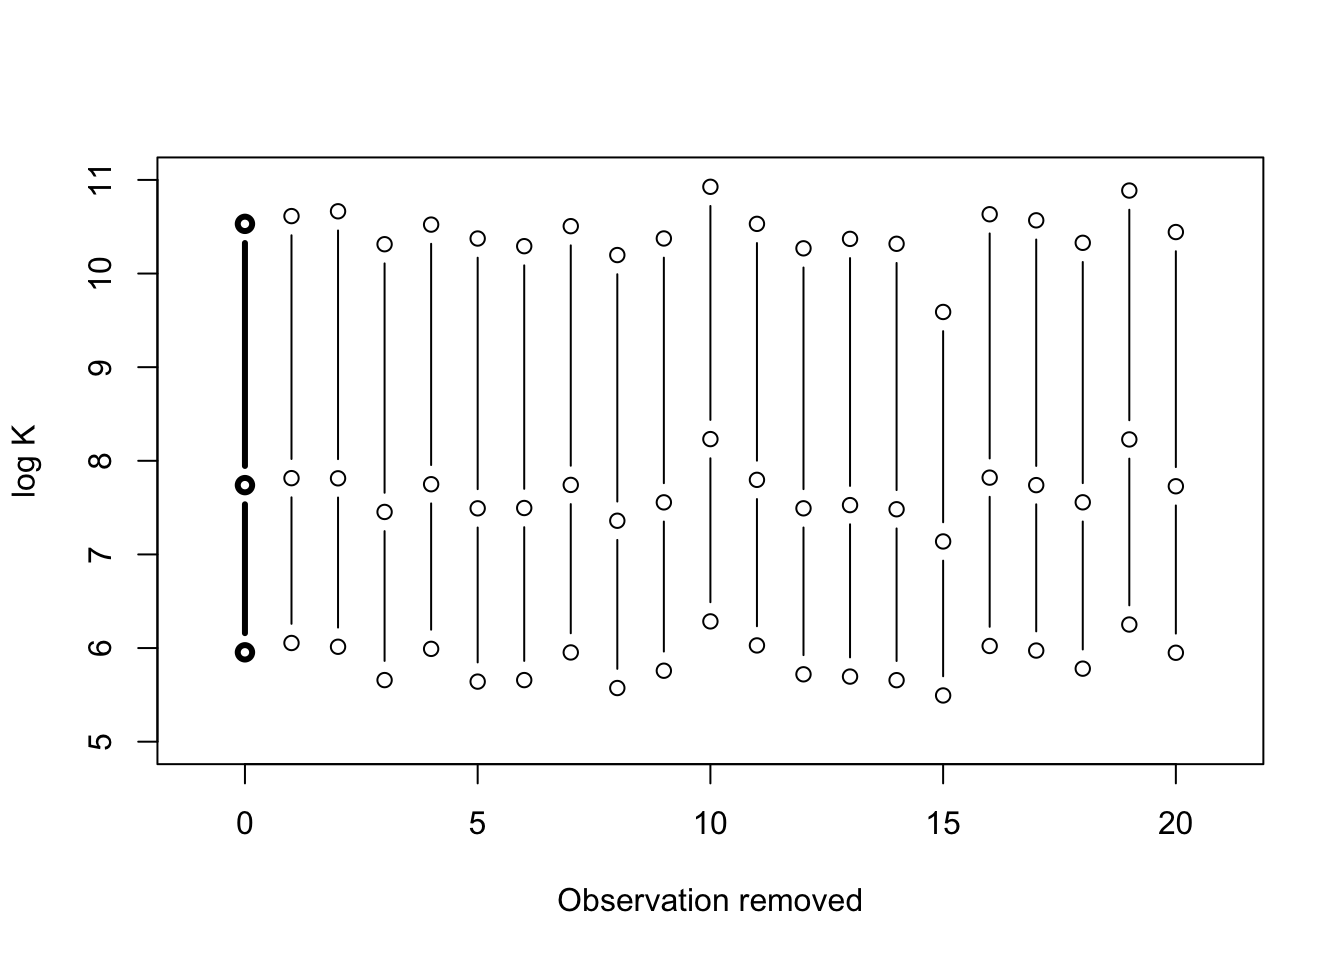
\includegraphics{bookdown-demo_files/figure-latex/unnamed-chunk-96-1.pdf}

\hypertarget{markov-chain-monte-carlo-methods}{%
\chapter{Markov Chain Monte Carlo Methods}\label{markov-chain-monte-carlo-methods}}

\hypertarget{introduction-to-discrete-markov-chains}{%
\section{Introduction to Discrete Markov Chains}\label{introduction-to-discrete-markov-chains}}

Illustration of sampling from a random walk distribution.

\begin{Shaded}
\begin{Highlighting}[]
\NormalTok{P }\OtherTok{\textless{}{-}} \FunctionTok{matrix}\NormalTok{(}\FunctionTok{c}\NormalTok{(.}\DecValTok{5}\NormalTok{, .}\DecValTok{5}\NormalTok{, }\DecValTok{0}\NormalTok{, }\DecValTok{0}\NormalTok{, }\DecValTok{0}\NormalTok{, }\DecValTok{0}\NormalTok{, }
\NormalTok{           .}\DecValTok{25}\NormalTok{, .}\DecValTok{5}\NormalTok{, .}\DecValTok{25}\NormalTok{, }\DecValTok{0}\NormalTok{, }\DecValTok{0}\NormalTok{, }\DecValTok{0}\NormalTok{, }
           \DecValTok{0}\NormalTok{, .}\DecValTok{25}\NormalTok{, .}\DecValTok{5}\NormalTok{, .}\DecValTok{25}\NormalTok{, }\DecValTok{0}\NormalTok{, }\DecValTok{0}\NormalTok{,}
           \DecValTok{0}\NormalTok{, }\DecValTok{0}\NormalTok{, .}\DecValTok{25}\NormalTok{, .}\DecValTok{5}\NormalTok{, .}\DecValTok{25}\NormalTok{, }\DecValTok{0}\NormalTok{, }
           \DecValTok{0}\NormalTok{, }\DecValTok{0}\NormalTok{, }\DecValTok{0}\NormalTok{, .}\DecValTok{25}\NormalTok{, .}\DecValTok{5}\NormalTok{, .}\DecValTok{25}\NormalTok{, }
           \DecValTok{0}\NormalTok{, }\DecValTok{0}\NormalTok{, }\DecValTok{0}\NormalTok{, }\DecValTok{0}\NormalTok{, .}\DecValTok{5}\NormalTok{, .}\DecValTok{5}\NormalTok{),}
           \AttributeTok{nrow=}\DecValTok{6}\NormalTok{, }\AttributeTok{ncol=}\DecValTok{6}\NormalTok{, }\AttributeTok{byrow=}\ConstantTok{TRUE}\NormalTok{)}
\NormalTok{ P}
\end{Highlighting}
\end{Shaded}

\begin{verbatim}
##      [,1] [,2] [,3] [,4] [,5] [,6]
## [1,] 0.50 0.50 0.00 0.00 0.00 0.00
## [2,] 0.25 0.50 0.25 0.00 0.00 0.00
## [3,] 0.00 0.25 0.50 0.25 0.00 0.00
## [4,] 0.00 0.00 0.25 0.50 0.25 0.00
## [5,] 0.00 0.00 0.00 0.25 0.50 0.25
## [6,] 0.00 0.00 0.00 0.00 0.50 0.50
\end{verbatim}

\begin{Shaded}
\begin{Highlighting}[]
\NormalTok{s }\OtherTok{\textless{}{-}} \FunctionTok{array}\NormalTok{(}\DecValTok{0}\NormalTok{, }\FunctionTok{c}\NormalTok{(}\DecValTok{50000}\NormalTok{, }\DecValTok{1}\NormalTok{))}
\NormalTok{s[}\DecValTok{1}\NormalTok{] }\OtherTok{\textless{}{-}} \DecValTok{3}
\ControlFlowTok{for}\NormalTok{ (j }\ControlFlowTok{in} \DecValTok{2}\SpecialCharTok{:}\DecValTok{50000}\NormalTok{)\{}
\NormalTok{   s[j] }\OtherTok{\textless{}{-}} \FunctionTok{sample}\NormalTok{(}\DecValTok{1}\SpecialCharTok{:}\DecValTok{6}\NormalTok{, }\AttributeTok{size=}\DecValTok{1}\NormalTok{, }\AttributeTok{prob=}\NormalTok{P[s[j }\SpecialCharTok{{-}} \DecValTok{1}\NormalTok{],])}
\NormalTok{\}}
\end{Highlighting}
\end{Shaded}

\begin{Shaded}
\begin{Highlighting}[]
\NormalTok{m }\OtherTok{\textless{}{-}} \FunctionTok{c}\NormalTok{(}\DecValTok{500}\NormalTok{, }\DecValTok{2000}\NormalTok{, }\DecValTok{8000}\NormalTok{, }\DecValTok{50000}\NormalTok{)}
\ControlFlowTok{for}\NormalTok{ (i }\ControlFlowTok{in} \DecValTok{1}\SpecialCharTok{:}\DecValTok{4}\NormalTok{)\{}
   \FunctionTok{print}\NormalTok{(}\FunctionTok{table}\NormalTok{(s[}\DecValTok{1}\SpecialCharTok{:}\NormalTok{m[i]]) }\SpecialCharTok{/}\NormalTok{ m[i])}
\NormalTok{\}}
\end{Highlighting}
\end{Shaded}

\begin{verbatim}
## 
##     1     2     3     4     5     6 
## 0.138 0.158 0.142 0.194 0.236 0.132 
## 
##      1      2      3      4      5      6 
## 0.1010 0.1895 0.1810 0.1905 0.2080 0.1300 
## 
##        1        2        3        4        5        6 
## 0.111250 0.209375 0.195000 0.190625 0.186625 0.107125 
## 
##       1       2       3       4       5       6 
## 0.10062 0.19684 0.20054 0.20030 0.19934 0.10236
\end{verbatim}

\begin{Shaded}
\begin{Highlighting}[]
\NormalTok{w }\OtherTok{\textless{}{-}} \FunctionTok{matrix}\NormalTok{(}\FunctionTok{c}\NormalTok{(.}\DecValTok{1}\NormalTok{, .}\DecValTok{2}\NormalTok{, .}\DecValTok{2}\NormalTok{, .}\DecValTok{2}\NormalTok{, .}\DecValTok{2}\NormalTok{, .}\DecValTok{1}\NormalTok{), }
            \AttributeTok{nrow=}\DecValTok{1}\NormalTok{, }\AttributeTok{ncol=}\DecValTok{6}\NormalTok{)}
\NormalTok{w }\SpecialCharTok{\%*\%}\NormalTok{ P}
\end{Highlighting}
\end{Shaded}

\begin{verbatim}
##      [,1] [,2] [,3] [,4] [,5] [,6]
## [1,]  0.1  0.2  0.2  0.2  0.2  0.1
\end{verbatim}

\hypertarget{learning-about-a-normal-population-from-grouped-data}{%
\section{Learning about a Normal Population from Grouped Data}\label{learning-about-a-normal-population-from-grouped-data}}

Have normally distributed data where the data is observed in grouped form. Consider the posterior of \((\mu, \log \sigma)\).

\begin{Shaded}
\begin{Highlighting}[]
\NormalTok{d }\OtherTok{\textless{}{-}} \FunctionTok{list}\NormalTok{(}\AttributeTok{int.lo=}\FunctionTok{c}\NormalTok{(}\SpecialCharTok{{-}}\ConstantTok{Inf}\NormalTok{, }\FunctionTok{seq}\NormalTok{(}\DecValTok{66}\NormalTok{, }\DecValTok{74}\NormalTok{, }\AttributeTok{by=}\DecValTok{2}\NormalTok{)),}
        \AttributeTok{int.hi=}\FunctionTok{c}\NormalTok{(}\FunctionTok{seq}\NormalTok{(}\DecValTok{66}\NormalTok{, }\DecValTok{74}\NormalTok{, }\AttributeTok{by=}\DecValTok{2}\NormalTok{), }\ConstantTok{Inf}\NormalTok{),}
        \AttributeTok{f=}\FunctionTok{c}\NormalTok{(}\DecValTok{14}\NormalTok{, }\DecValTok{30}\NormalTok{, }\DecValTok{49}\NormalTok{, }\DecValTok{70}\NormalTok{, }\DecValTok{33}\NormalTok{, }\DecValTok{15}\NormalTok{))}
\end{Highlighting}
\end{Shaded}

\begin{Shaded}
\begin{Highlighting}[]
\NormalTok{y }\OtherTok{\textless{}{-}} \FunctionTok{c}\NormalTok{(}\FunctionTok{rep}\NormalTok{(}\DecValTok{65}\NormalTok{,}\DecValTok{14}\NormalTok{), }\FunctionTok{rep}\NormalTok{(}\DecValTok{67}\NormalTok{,}\DecValTok{30}\NormalTok{), }\FunctionTok{rep}\NormalTok{(}\DecValTok{69}\NormalTok{,}\DecValTok{49}\NormalTok{),}
       \FunctionTok{rep}\NormalTok{(}\DecValTok{71}\NormalTok{,}\DecValTok{70}\NormalTok{), }\FunctionTok{rep}\NormalTok{(}\DecValTok{73}\NormalTok{,}\DecValTok{33}\NormalTok{), }\FunctionTok{rep}\NormalTok{(}\DecValTok{75}\NormalTok{,}\DecValTok{15}\NormalTok{))}
\FunctionTok{mean}\NormalTok{(y)}
\end{Highlighting}
\end{Shaded}

\begin{verbatim}
## [1] 70.16588
\end{verbatim}

\begin{Shaded}
\begin{Highlighting}[]
\FunctionTok{log}\NormalTok{(}\FunctionTok{sd}\NormalTok{(y))}
\end{Highlighting}
\end{Shaded}

\begin{verbatim}
## [1] 0.9504117
\end{verbatim}

First obtain normal approximation to posterior.

\begin{Shaded}
\begin{Highlighting}[]
\NormalTok{start }\OtherTok{\textless{}{-}} \FunctionTok{c}\NormalTok{(}\DecValTok{70}\NormalTok{, }\DecValTok{1}\NormalTok{)}
\NormalTok{fit }\OtherTok{\textless{}{-}} \FunctionTok{laplace}\NormalTok{(groupeddatapost, start, d)}
\NormalTok{fit}
\end{Highlighting}
\end{Shaded}

\begin{verbatim}
## $mode
## [1] 70.169880  0.973644
## 
## $var
##              [,1]         [,2]
## [1,] 3.534713e-02 3.520776e-05
## [2,] 3.520776e-05 3.146470e-03
## 
## $int
## [1] -350.6305
## 
## $converge
## [1] TRUE
\end{verbatim}

Now use a Metropolis (random walk) MCMC algorithm.

\begin{Shaded}
\begin{Highlighting}[]
\NormalTok{modal.sds }\OtherTok{\textless{}{-}} \FunctionTok{sqrt}\NormalTok{(}\FunctionTok{diag}\NormalTok{(fit}\SpecialCharTok{$}\NormalTok{var))}
\NormalTok{proposal }\OtherTok{\textless{}{-}} \FunctionTok{list}\NormalTok{(}\AttributeTok{var=}\NormalTok{fit}\SpecialCharTok{$}\NormalTok{var, }\AttributeTok{scale=}\DecValTok{2}\NormalTok{)}
\NormalTok{fit2 }\OtherTok{\textless{}{-}} \FunctionTok{rwmetrop}\NormalTok{(groupeddatapost,}
\NormalTok{                 proposal,}
\NormalTok{                 start,}
                 \DecValTok{10000}\NormalTok{, d)}
\end{Highlighting}
\end{Shaded}

\begin{Shaded}
\begin{Highlighting}[]
\NormalTok{fit2}\SpecialCharTok{$}\NormalTok{accept}
\end{Highlighting}
\end{Shaded}

\begin{verbatim}
## [1] 0.3011
\end{verbatim}

\begin{Shaded}
\begin{Highlighting}[]
\NormalTok{post.means }\OtherTok{\textless{}{-}} \FunctionTok{apply}\NormalTok{(fit2}\SpecialCharTok{$}\NormalTok{par, }\DecValTok{2}\NormalTok{, mean)}
\NormalTok{post.sds }\OtherTok{\textless{}{-}} \FunctionTok{apply}\NormalTok{(fit2}\SpecialCharTok{$}\NormalTok{par, }\DecValTok{2}\NormalTok{, sd)}
\FunctionTok{cbind}\NormalTok{(}\FunctionTok{c}\NormalTok{(fit}\SpecialCharTok{$}\NormalTok{mode), modal.sds)}
\end{Highlighting}
\end{Shaded}

\begin{verbatim}
##                 modal.sds
## [1,] 70.169880 0.18800834
## [2,]  0.973644 0.05609341
\end{verbatim}

\begin{Shaded}
\begin{Highlighting}[]
\FunctionTok{cbind}\NormalTok{(post.means, post.sds)}
\end{Highlighting}
\end{Shaded}

\begin{verbatim}
##      post.means   post.sds
## [1,] 70.1683845 0.18297635
## [2,]  0.9803531 0.05545176
\end{verbatim}

\begin{Shaded}
\begin{Highlighting}[]
\FunctionTok{mycontour}\NormalTok{(groupeddatapost,}
          \FunctionTok{c}\NormalTok{(}\DecValTok{69}\NormalTok{, }\DecValTok{71}\NormalTok{, .}\DecValTok{6}\NormalTok{, }\FloatTok{1.3}\NormalTok{), d,}
       \AttributeTok{xlab=}\StringTok{"mu"}\NormalTok{,}\AttributeTok{ylab=}\StringTok{"log sigma"}\NormalTok{)}
\FunctionTok{points}\NormalTok{(fit2}\SpecialCharTok{$}\NormalTok{par[}\DecValTok{5001}\SpecialCharTok{:}\DecValTok{10000}\NormalTok{, }\DecValTok{1}\NormalTok{],}
\NormalTok{       fit2}\SpecialCharTok{$}\NormalTok{par[}\DecValTok{5001}\SpecialCharTok{:}\DecValTok{10000}\NormalTok{, }\DecValTok{2}\NormalTok{])}
\end{Highlighting}
\end{Shaded}

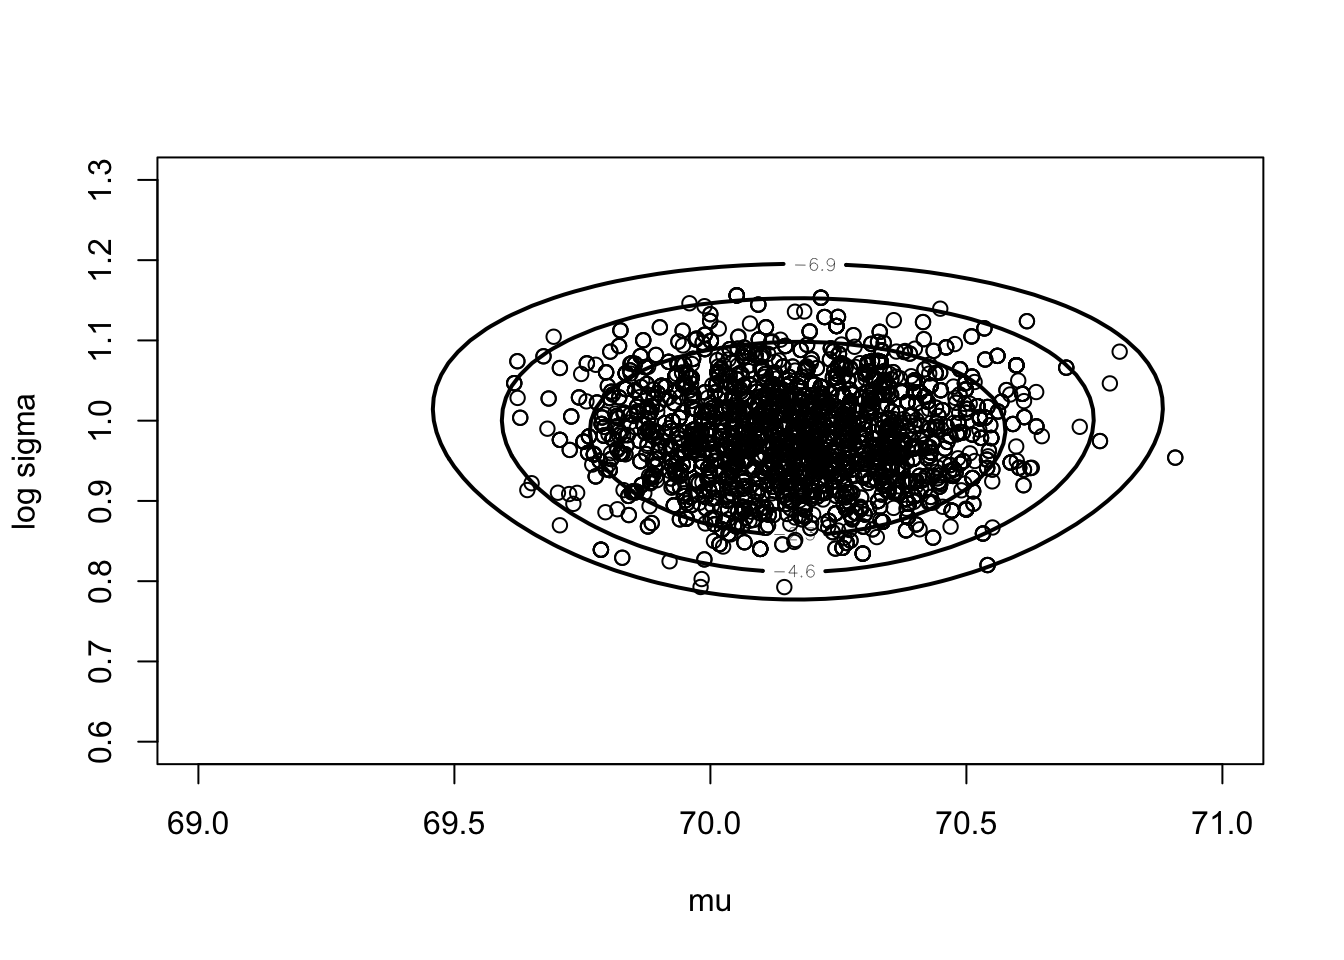
\includegraphics{bookdown-demo_files/figure-latex/unnamed-chunk-108-1.pdf}

\hypertarget{example-of-output-analysis}{%
\section{Example of Output Analysis}\label{example-of-output-analysis}}

Illustrate MCMC diagnositics for different Metropolis chains with different proposal widths.

\begin{Shaded}
\begin{Highlighting}[]
\NormalTok{d }\OtherTok{\textless{}{-}} \FunctionTok{list}\NormalTok{(}\AttributeTok{int.lo=}\FunctionTok{c}\NormalTok{(}\SpecialCharTok{{-}}\ConstantTok{Inf}\NormalTok{, }\FunctionTok{seq}\NormalTok{(}\DecValTok{66}\NormalTok{, }\DecValTok{74}\NormalTok{, }\AttributeTok{by=}\DecValTok{2}\NormalTok{)),}
        \AttributeTok{int.hi=}\FunctionTok{c}\NormalTok{(}\FunctionTok{seq}\NormalTok{(}\DecValTok{66}\NormalTok{, }\DecValTok{74}\NormalTok{, }\AttributeTok{by=}\DecValTok{2}\NormalTok{), }\ConstantTok{Inf}\NormalTok{),}
        \AttributeTok{f=}\FunctionTok{c}\NormalTok{(}\DecValTok{14}\NormalTok{, }\DecValTok{30}\NormalTok{, }\DecValTok{49}\NormalTok{, }\DecValTok{70}\NormalTok{, }\DecValTok{33}\NormalTok{, }\DecValTok{15}\NormalTok{))}
\end{Highlighting}
\end{Shaded}

\begin{Shaded}
\begin{Highlighting}[]
\FunctionTok{library}\NormalTok{(coda)}
\FunctionTok{library}\NormalTok{(lattice)}
\end{Highlighting}
\end{Shaded}

\begin{Shaded}
\begin{Highlighting}[]
\NormalTok{start }\OtherTok{\textless{}{-}} \FunctionTok{c}\NormalTok{(}\DecValTok{70}\NormalTok{,}\DecValTok{1}\NormalTok{)}
\NormalTok{ fit }\OtherTok{\textless{}{-}} \FunctionTok{laplace}\NormalTok{(groupeddatapost, start, d)}
\end{Highlighting}
\end{Shaded}

\begin{Shaded}
\begin{Highlighting}[]
\NormalTok{start }\OtherTok{\textless{}{-}} \FunctionTok{c}\NormalTok{(}\DecValTok{65}\NormalTok{,}\DecValTok{1}\NormalTok{)}
\NormalTok{ proposal }\OtherTok{\textless{}{-}} \FunctionTok{list}\NormalTok{(}\AttributeTok{var=}\NormalTok{fit}\SpecialCharTok{$}\NormalTok{var, }\AttributeTok{scale=}\FloatTok{0.2}\NormalTok{)}
\NormalTok{ bayesfit }\OtherTok{\textless{}{-}} \FunctionTok{rwmetrop}\NormalTok{(groupeddatapost,}
\NormalTok{                      proposal,}
\NormalTok{                      start,}
                      \DecValTok{10000}\NormalTok{, d)}
\end{Highlighting}
\end{Shaded}

\begin{Shaded}
\begin{Highlighting}[]
\FunctionTok{dimnames}\NormalTok{(bayesfit}\SpecialCharTok{$}\NormalTok{par)[[}\DecValTok{2}\NormalTok{]] }\OtherTok{\textless{}{-}} \FunctionTok{c}\NormalTok{(}\StringTok{"mu"}\NormalTok{, }\StringTok{"log sigma"}\NormalTok{)}
 \FunctionTok{xyplot}\NormalTok{(}\FunctionTok{mcmc}\NormalTok{(bayesfit}\SpecialCharTok{$}\NormalTok{par[}\SpecialCharTok{{-}}\FunctionTok{c}\NormalTok{(}\DecValTok{1}\SpecialCharTok{:}\DecValTok{2000}\NormalTok{), ]),}
        \AttributeTok{col=}\StringTok{"black"}\NormalTok{)}
\end{Highlighting}
\end{Shaded}

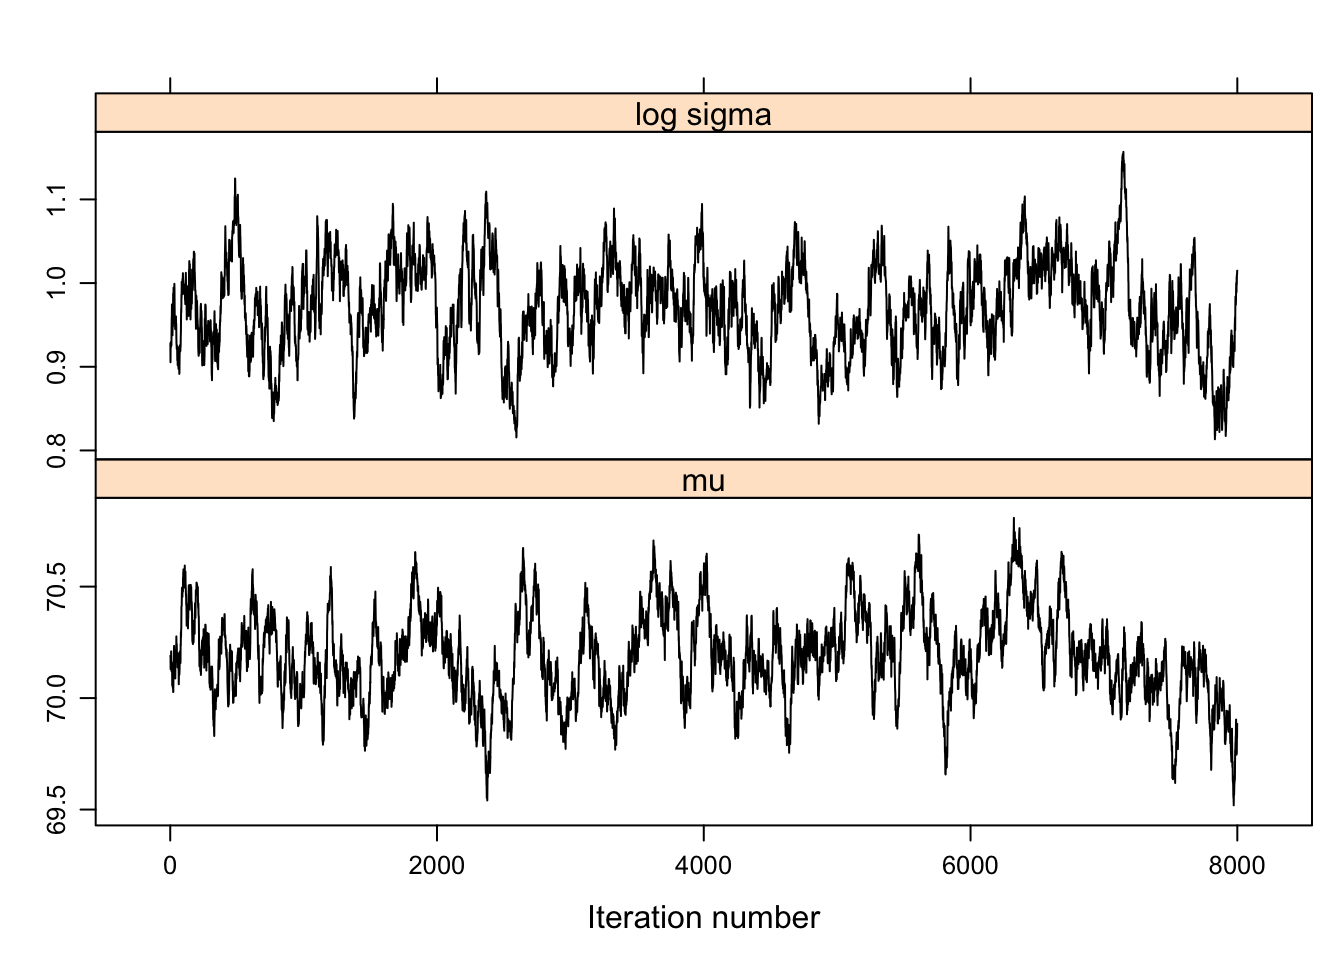
\includegraphics{bookdown-demo_files/figure-latex/unnamed-chunk-113-1.pdf}

\begin{Shaded}
\begin{Highlighting}[]
\FunctionTok{par}\NormalTok{(}\AttributeTok{mfrow=}\FunctionTok{c}\NormalTok{(}\DecValTok{2}\NormalTok{, }\DecValTok{1}\NormalTok{))}
 \FunctionTok{autocorr.plot}\NormalTok{(}\FunctionTok{mcmc}\NormalTok{(bayesfit}\SpecialCharTok{$}\NormalTok{par[}\SpecialCharTok{{-}}\FunctionTok{c}\NormalTok{(}\DecValTok{1}\SpecialCharTok{:}\DecValTok{2000}\NormalTok{), ]),}
               \AttributeTok{auto.layout=}\ConstantTok{FALSE}\NormalTok{)}
\end{Highlighting}
\end{Shaded}

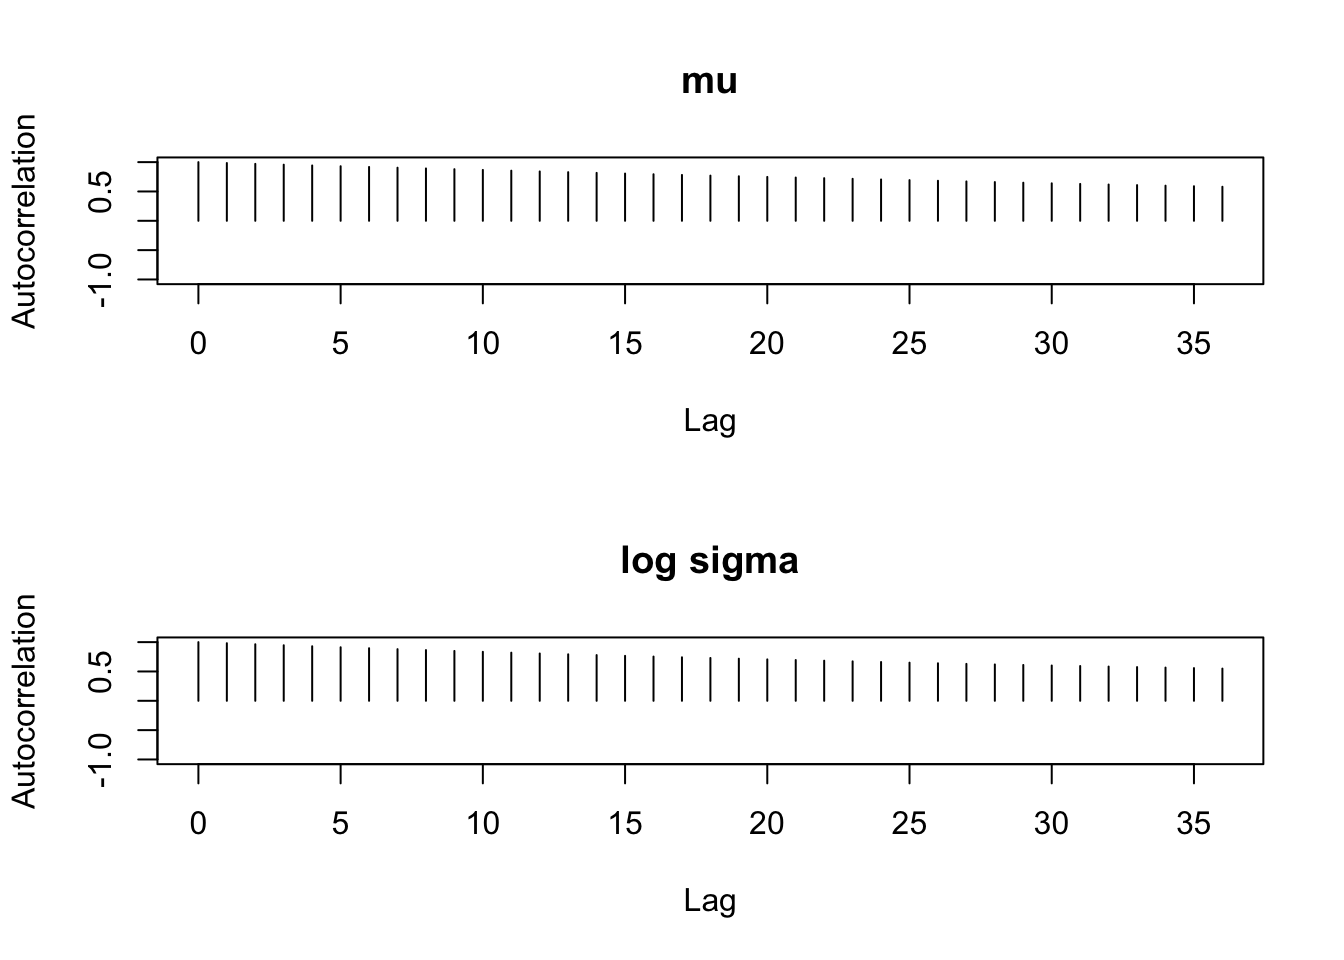
\includegraphics{bookdown-demo_files/figure-latex/unnamed-chunk-114-1.pdf}

\begin{Shaded}
\begin{Highlighting}[]
 \FunctionTok{summary}\NormalTok{(}\FunctionTok{mcmc}\NormalTok{(bayesfit}\SpecialCharTok{$}\NormalTok{par[}\SpecialCharTok{{-}}\FunctionTok{c}\NormalTok{(}\DecValTok{1}\SpecialCharTok{:}\DecValTok{2000}\NormalTok{), ]))}
\end{Highlighting}
\end{Shaded}

\begin{verbatim}
## 
## Iterations = 1:8000
## Thinning interval = 1 
## Number of chains = 1 
## Sample size per chain = 8000 
## 
## 1. Empirical mean and standard deviation for each variable,
##    plus standard error of the mean:
## 
##              Mean      SD  Naive SE Time-series SE
## mu        70.1703 0.21342 0.0023861       0.028804
## log sigma  0.9774 0.05308 0.0005934       0.005875
## 
## 2. Quantiles for each variable:
## 
##              2.5%     25%     50%    75%  97.5%
## mu        69.7478 70.0242 70.1792 70.316 70.589
## log sigma  0.8756  0.9395  0.9761  1.017  1.076
\end{verbatim}

\begin{Shaded}
\begin{Highlighting}[]
 \FunctionTok{batchSE}\NormalTok{(}\FunctionTok{mcmc}\NormalTok{(bayesfit}\SpecialCharTok{$}\NormalTok{par[}\SpecialCharTok{{-}}\FunctionTok{c}\NormalTok{(}\DecValTok{1}\SpecialCharTok{:}\DecValTok{2000}\NormalTok{), ]),}
         \AttributeTok{batchSize=}\DecValTok{50}\NormalTok{)}
\end{Highlighting}
\end{Shaded}

\begin{verbatim}
##          mu   log sigma 
## 0.015097003 0.003629486
\end{verbatim}

\begin{Shaded}
\begin{Highlighting}[]
\NormalTok{start }\OtherTok{\textless{}{-}} \FunctionTok{c}\NormalTok{(}\DecValTok{70}\NormalTok{,}\DecValTok{1}\NormalTok{)}
\NormalTok{ proposal }\OtherTok{\textless{}{-}} \FunctionTok{list}\NormalTok{(}\AttributeTok{var=}\NormalTok{fit}\SpecialCharTok{$}\NormalTok{var, }\AttributeTok{scale=}\FloatTok{2.0}\NormalTok{)}
\NormalTok{ bayesfit }\OtherTok{\textless{}{-}} \FunctionTok{rwmetrop}\NormalTok{(groupeddatapost, }
\NormalTok{                      proposal, }
\NormalTok{                      start,}
                      \DecValTok{10000}\NormalTok{, d)}
\end{Highlighting}
\end{Shaded}

\begin{Shaded}
\begin{Highlighting}[]
\FunctionTok{dimnames}\NormalTok{(bayesfit}\SpecialCharTok{$}\NormalTok{par)[[}\DecValTok{2}\NormalTok{]] }\OtherTok{\textless{}{-}} \FunctionTok{c}\NormalTok{(}\StringTok{"mu"}\NormalTok{, }\StringTok{"log sigma"}\NormalTok{)}
\NormalTok{sim.parameters }\OtherTok{\textless{}{-}} \FunctionTok{mcmc}\NormalTok{(bayesfit}\SpecialCharTok{$}\NormalTok{par[}\SpecialCharTok{{-}}\FunctionTok{c}\NormalTok{(}\DecValTok{1}\SpecialCharTok{:}\DecValTok{2000}\NormalTok{), ])}
 \FunctionTok{xyplot}\NormalTok{(}\FunctionTok{mcmc}\NormalTok{(bayesfit}\SpecialCharTok{$}\NormalTok{par[}\SpecialCharTok{{-}}\FunctionTok{c}\NormalTok{(}\DecValTok{1}\SpecialCharTok{:}\DecValTok{2000}\NormalTok{), ]), }
        \AttributeTok{col=}\StringTok{"black"}\NormalTok{)}
\end{Highlighting}
\end{Shaded}

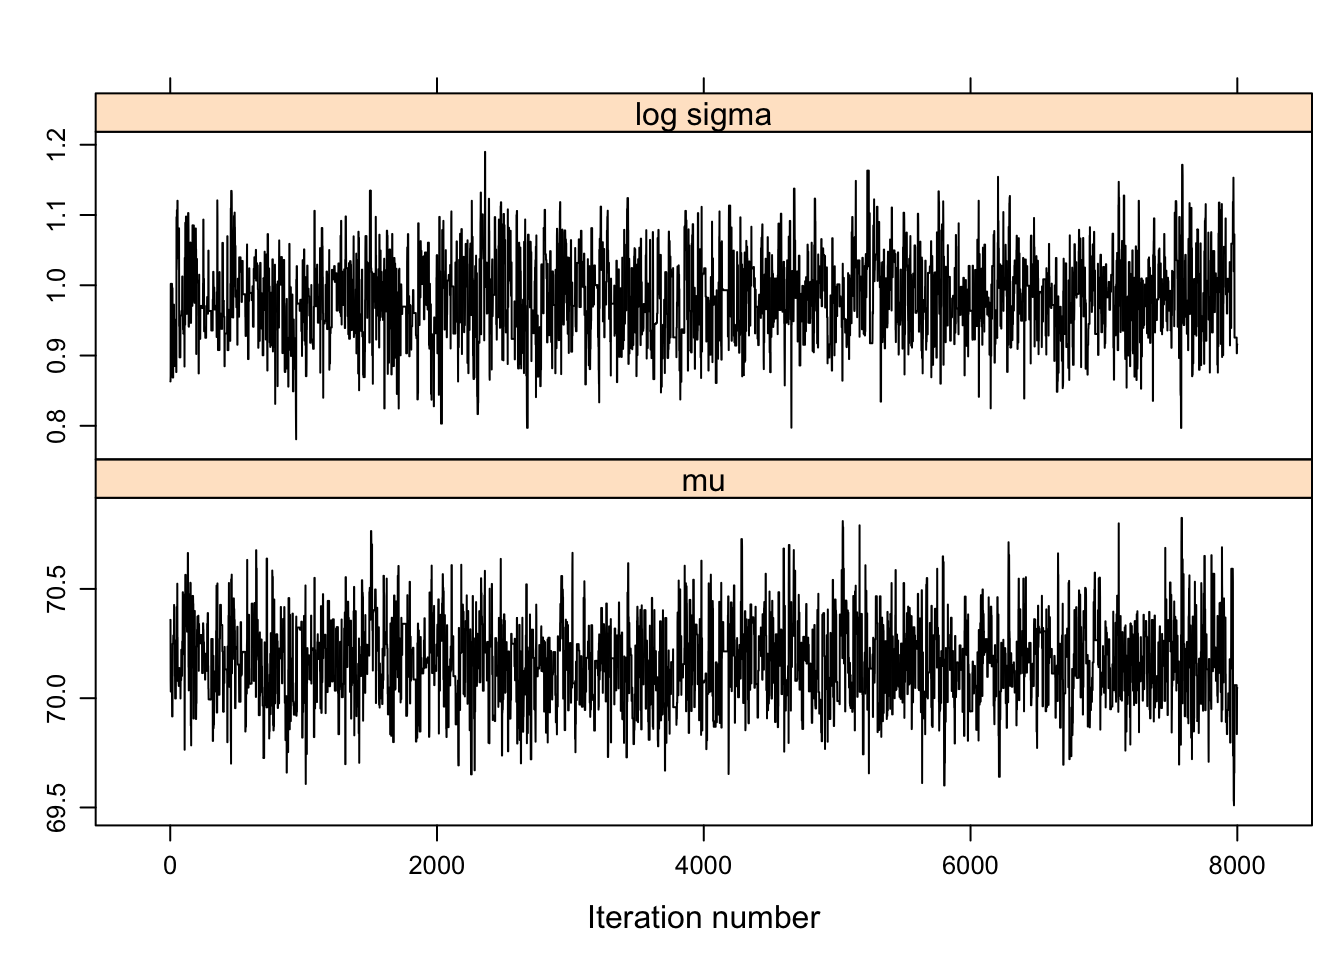
\includegraphics{bookdown-demo_files/figure-latex/unnamed-chunk-116-1.pdf}

\begin{Shaded}
\begin{Highlighting}[]
\FunctionTok{par}\NormalTok{(}\AttributeTok{mfrow=}\FunctionTok{c}\NormalTok{(}\DecValTok{2}\NormalTok{,}\DecValTok{1}\NormalTok{))}
 \FunctionTok{autocorr.plot}\NormalTok{(sim.parameters,}\AttributeTok{auto.layout=}\ConstantTok{FALSE}\NormalTok{)}
\end{Highlighting}
\end{Shaded}

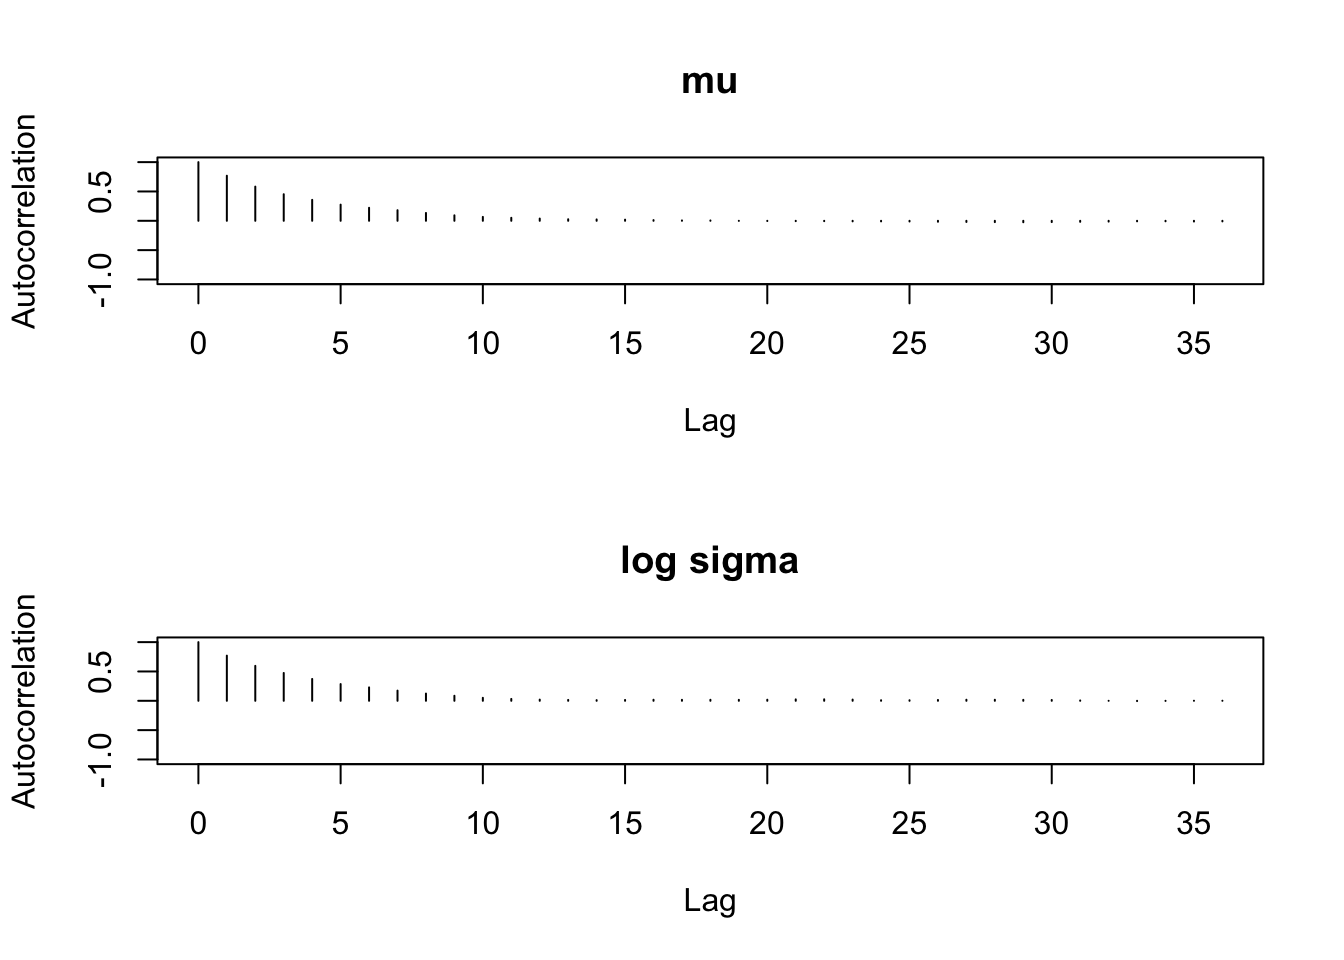
\includegraphics{bookdown-demo_files/figure-latex/unnamed-chunk-117-1.pdf}

\begin{Shaded}
\begin{Highlighting}[]
 \FunctionTok{summary}\NormalTok{(sim.parameters)}
\end{Highlighting}
\end{Shaded}

\begin{verbatim}
## 
## Iterations = 1:8000
## Thinning interval = 1 
## Number of chains = 1 
## Sample size per chain = 8000 
## 
## 1. Empirical mean and standard deviation for each variable,
##    plus standard error of the mean:
## 
##              Mean      SD  Naive SE Time-series SE
## mu        70.1768 0.19412 0.0021703       0.005967
## log sigma  0.9795 0.05732 0.0006409       0.001795
## 
## 2. Quantiles for each variable:
## 
##              2.5%     25%     50%    75%  97.5%
## mu        69.7923 70.0437 70.1745 70.309 70.556
## log sigma  0.8677  0.9398  0.9804  1.019  1.088
\end{verbatim}

\begin{Shaded}
\begin{Highlighting}[]
 \FunctionTok{batchSE}\NormalTok{(sim.parameters, }\AttributeTok{batchSize=}\DecValTok{50}\NormalTok{)}
\end{Highlighting}
\end{Shaded}

\begin{verbatim}
##          mu   log sigma 
## 0.006082428 0.001632771
\end{verbatim}

\hypertarget{modeling-data-with-cauchy-errors}{%
\section{Modeling Data with Cauchy Errors}\label{modeling-data-with-cauchy-errors}}

Assuming data that is sampled from a Cauchy density with a noninformative prior placed on the location and scale parameters.

\begin{Shaded}
\begin{Highlighting}[]
\FunctionTok{mean}\NormalTok{(darwin}\SpecialCharTok{$}\NormalTok{difference)}
\end{Highlighting}
\end{Shaded}

\begin{verbatim}
## [1] 21.66667
\end{verbatim}

\begin{Shaded}
\begin{Highlighting}[]
\FunctionTok{log}\NormalTok{(}\FunctionTok{sd}\NormalTok{(darwin}\SpecialCharTok{$}\NormalTok{difference))}
\end{Highlighting}
\end{Shaded}

\begin{verbatim}
## [1] 3.65253
\end{verbatim}

First illustrate normal approximation.

\begin{Shaded}
\begin{Highlighting}[]
\FunctionTok{laplace}\NormalTok{(cauchyerrorpost, }
        \FunctionTok{c}\NormalTok{(}\FloatTok{21.6}\NormalTok{, }\FloatTok{3.6}\NormalTok{), }
\NormalTok{        darwin}\SpecialCharTok{$}\NormalTok{difference)}
\end{Highlighting}
\end{Shaded}

\begin{verbatim}
## $mode
## [1] 24.701745  2.772619
## 
## $var
##            [,1]      [,2]
## [1,] 34.9600525 0.3672899
## [2,]  0.3672899 0.1378279
## 
## $int
## [1] -73.2404
## 
## $converge
## [1] TRUE
\end{verbatim}

\begin{Shaded}
\begin{Highlighting}[]
\FunctionTok{laplace}\NormalTok{(cauchyerrorpost, }
\NormalTok{        .}\DecValTok{1} \SpecialCharTok{*} \FunctionTok{c}\NormalTok{(}\FloatTok{21.6}\NormalTok{,}\FloatTok{3.6}\NormalTok{), }
\NormalTok{        darwin}\SpecialCharTok{$}\NormalTok{difference)}\SpecialCharTok{$}\NormalTok{mode}
\end{Highlighting}
\end{Shaded}

\begin{verbatim}
## [1] 24.698151  2.772345
\end{verbatim}

\begin{Shaded}
\begin{Highlighting}[]
\FunctionTok{c}\NormalTok{(}\FloatTok{24.7} \SpecialCharTok{{-}} \DecValTok{4} \SpecialCharTok{*} \FunctionTok{sqrt}\NormalTok{(}\FloatTok{34.96}\NormalTok{), }\FloatTok{24.7} \SpecialCharTok{+} \DecValTok{4} \SpecialCharTok{*} \FunctionTok{sqrt}\NormalTok{(}\FloatTok{34.96}\NormalTok{))}
\end{Highlighting}
\end{Shaded}

\begin{verbatim}
## [1]  1.049207 48.350793
\end{verbatim}

\begin{Shaded}
\begin{Highlighting}[]
\FunctionTok{c}\NormalTok{(}\FloatTok{2.77} \SpecialCharTok{{-}} \DecValTok{4} \SpecialCharTok{*} \FunctionTok{sqrt}\NormalTok{(.}\DecValTok{138}\NormalTok{), }\FloatTok{2.77} \SpecialCharTok{+} \DecValTok{4} \SpecialCharTok{*} \FunctionTok{sqrt}\NormalTok{(.}\DecValTok{138}\NormalTok{))}
\end{Highlighting}
\end{Shaded}

\begin{verbatim}
## [1] 1.284066 4.255934
\end{verbatim}

\begin{Shaded}
\begin{Highlighting}[]
\FunctionTok{mycontour}\NormalTok{(cauchyerrorpost,}
          \FunctionTok{c}\NormalTok{(}\SpecialCharTok{{-}}\DecValTok{10}\NormalTok{, }\DecValTok{60}\NormalTok{, }\DecValTok{1}\NormalTok{, }\FloatTok{4.5}\NormalTok{),}
\NormalTok{          darwin}\SpecialCharTok{$}\NormalTok{difference,}
          \AttributeTok{xlab=}\StringTok{"mu"}\NormalTok{, }\AttributeTok{ylab=}\StringTok{"log sigma"}\NormalTok{)}
\end{Highlighting}
\end{Shaded}

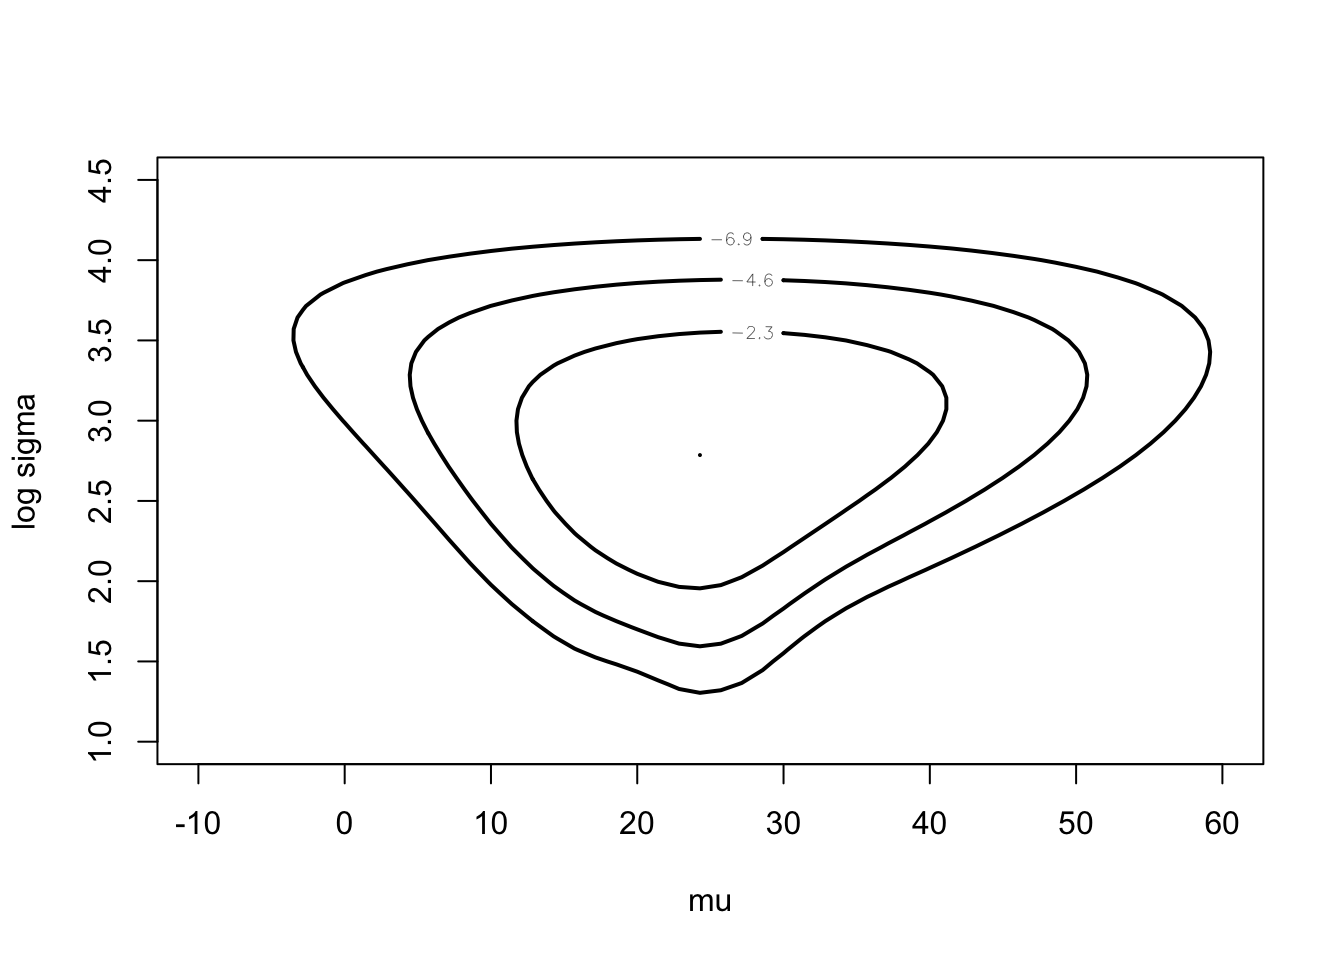
\includegraphics{bookdown-demo_files/figure-latex/unnamed-chunk-123-1.pdf}

\begin{Shaded}
\begin{Highlighting}[]
\NormalTok{fitlaplace }\OtherTok{\textless{}{-}} \FunctionTok{laplace}\NormalTok{(cauchyerrorpost,}
                      \FunctionTok{c}\NormalTok{(}\FloatTok{21.6}\NormalTok{, }\FloatTok{3.6}\NormalTok{), }
\NormalTok{                      darwin}\SpecialCharTok{$}\NormalTok{difference)}
\end{Highlighting}
\end{Shaded}

\begin{Shaded}
\begin{Highlighting}[]
\FunctionTok{mycontour}\NormalTok{(lbinorm,}
          \FunctionTok{c}\NormalTok{(}\SpecialCharTok{{-}}\DecValTok{10}\NormalTok{, }\DecValTok{60}\NormalTok{, }\DecValTok{1}\NormalTok{, }\FloatTok{4.5}\NormalTok{),}
          \FunctionTok{list}\NormalTok{(}\AttributeTok{m=}\NormalTok{fitlaplace}\SpecialCharTok{$}\NormalTok{mode,}
               \AttributeTok{v=}\NormalTok{fitlaplace}\SpecialCharTok{$}\NormalTok{var), }
           \AttributeTok{xlab=}\StringTok{"mu"}\NormalTok{,}\AttributeTok{ylab=}\StringTok{"log sigma"}\NormalTok{)}
\end{Highlighting}
\end{Shaded}

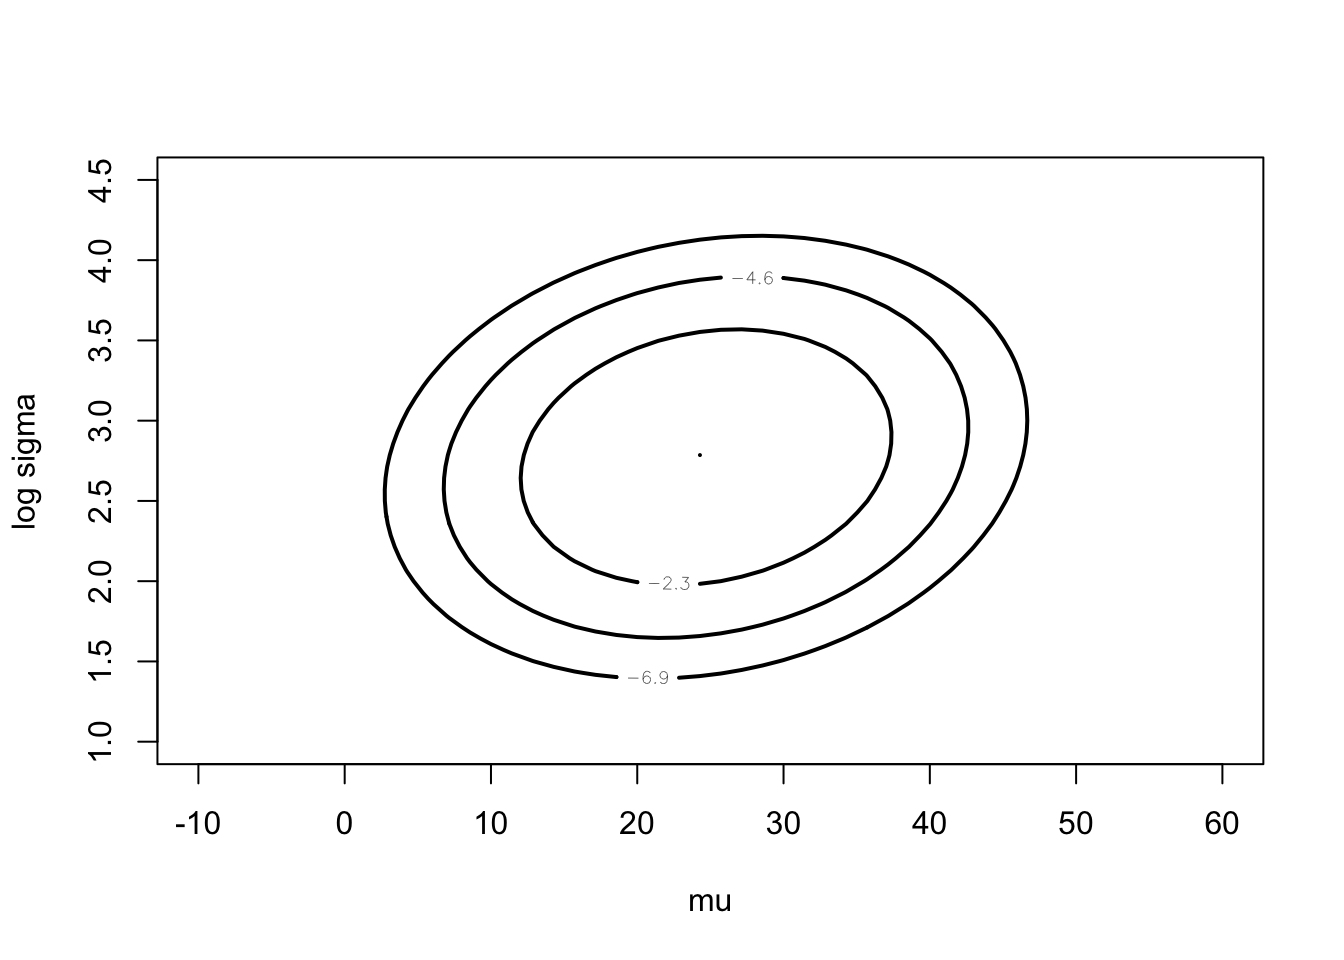
\includegraphics{bookdown-demo_files/figure-latex/unnamed-chunk-125-1.pdf}

Next illustrate random walk Metropolis.

\begin{Shaded}
\begin{Highlighting}[]
\NormalTok{proposal }\OtherTok{\textless{}{-}} \FunctionTok{list}\NormalTok{(}\AttributeTok{var=}\NormalTok{fitlaplace}\SpecialCharTok{$}\NormalTok{var, }\AttributeTok{scale=}\FloatTok{2.5}\NormalTok{)}
\NormalTok{start }\OtherTok{\textless{}{-}} \FunctionTok{c}\NormalTok{(}\DecValTok{20}\NormalTok{, }\DecValTok{3}\NormalTok{)}
\NormalTok{m }\OtherTok{\textless{}{-}} \DecValTok{1000}
\NormalTok{s }\OtherTok{\textless{}{-}} \FunctionTok{rwmetrop}\NormalTok{(cauchyerrorpost, proposal, }
\NormalTok{              start, m, darwin}\SpecialCharTok{$}\NormalTok{difference)}
\end{Highlighting}
\end{Shaded}

\begin{Shaded}
\begin{Highlighting}[]
\FunctionTok{mycontour}\NormalTok{(cauchyerrorpost, }
          \FunctionTok{c}\NormalTok{(}\SpecialCharTok{{-}}\DecValTok{10}\NormalTok{, }\DecValTok{60}\NormalTok{, }\DecValTok{1}\NormalTok{, }\FloatTok{4.5}\NormalTok{),}
\NormalTok{          darwin}\SpecialCharTok{$}\NormalTok{difference,}
          \AttributeTok{xlab=}\StringTok{"mu"}\NormalTok{, }\AttributeTok{ylab=}\StringTok{"log sigma"}\NormalTok{)}
 \FunctionTok{points}\NormalTok{(s}\SpecialCharTok{$}\NormalTok{par[,}\DecValTok{1}\NormalTok{], s}\SpecialCharTok{$}\NormalTok{par[,}\DecValTok{2}\NormalTok{])}
\end{Highlighting}
\end{Shaded}

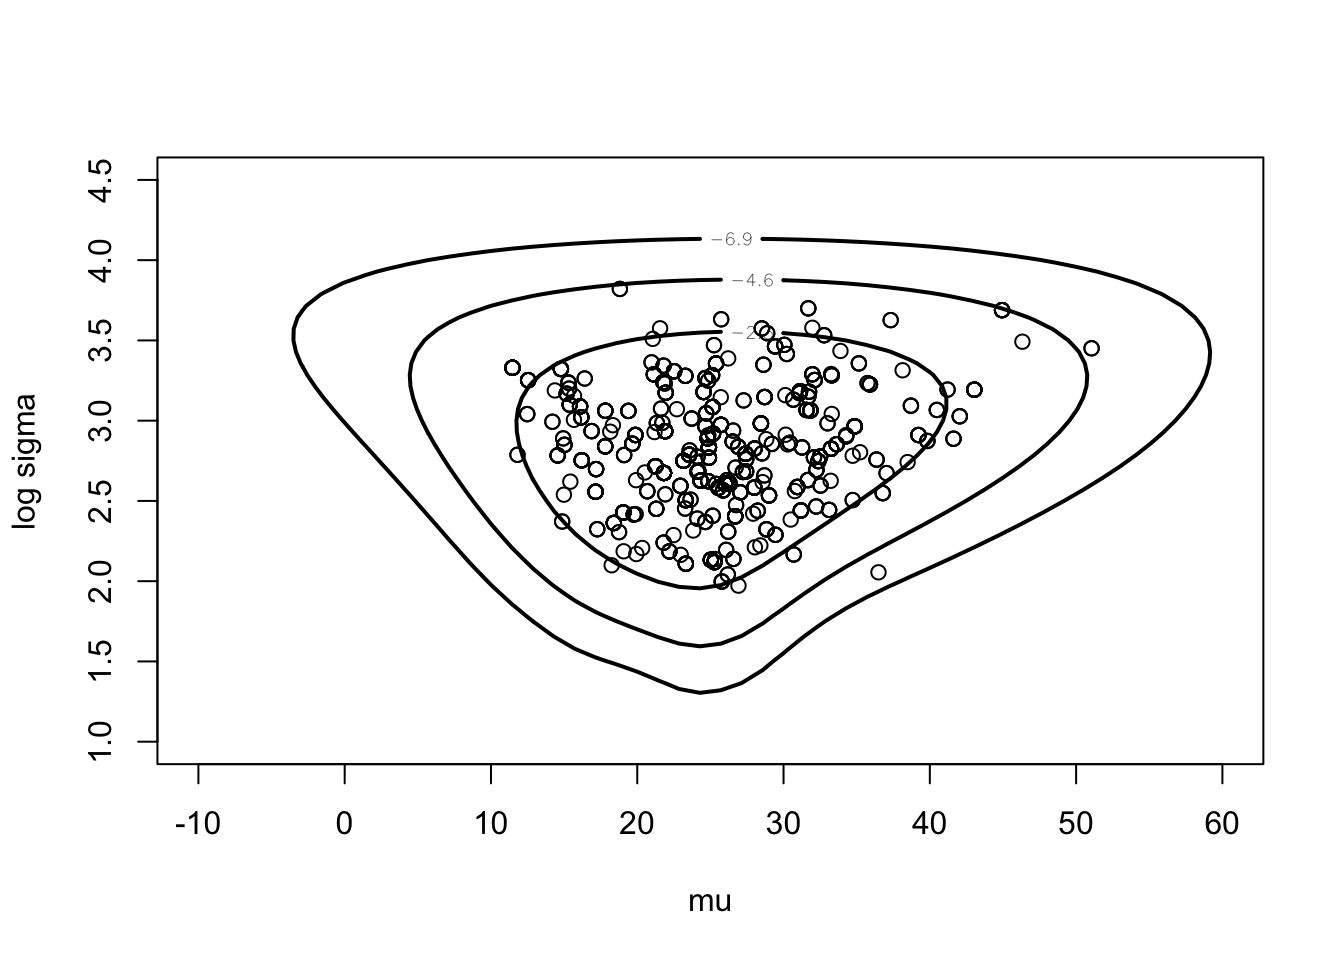
\includegraphics{bookdown-demo_files/figure-latex/unnamed-chunk-127-1.pdf}

\begin{Shaded}
\begin{Highlighting}[]
\NormalTok{fitgrid }\OtherTok{\textless{}{-}} \FunctionTok{simcontour}\NormalTok{(cauchyerrorpost,}
                      \FunctionTok{c}\NormalTok{(}\SpecialCharTok{{-}}\DecValTok{10}\NormalTok{,}\DecValTok{60}\NormalTok{,}\DecValTok{1}\NormalTok{,}\FloatTok{4.5}\NormalTok{),}
\NormalTok{                      darwin}\SpecialCharTok{$}\NormalTok{difference,}
                      \DecValTok{50000}\NormalTok{)}
\end{Highlighting}
\end{Shaded}

\begin{Shaded}
\begin{Highlighting}[]
\NormalTok{proposal }\OtherTok{\textless{}{-}} \FunctionTok{list}\NormalTok{(}\AttributeTok{var=}\NormalTok{fitlaplace}\SpecialCharTok{$}\NormalTok{var, }
                 \AttributeTok{scale=}\FloatTok{2.5}\NormalTok{)}
\NormalTok{                 start}\OtherTok{=}\FunctionTok{c}\NormalTok{(}\DecValTok{20}\NormalTok{, }\DecValTok{3}\NormalTok{)}
\NormalTok{fitrw}\OtherTok{=}\FunctionTok{rwmetrop}\NormalTok{(cauchyerrorpost,}
\NormalTok{                proposal, }
\NormalTok{                start,}
                \DecValTok{50000}\NormalTok{,}
\NormalTok{                darwin}\SpecialCharTok{$}\NormalTok{difference)}
\end{Highlighting}
\end{Shaded}

Illustrate metropolis-hastings independence chain.

\begin{Shaded}
\begin{Highlighting}[]
\NormalTok{proposal2 }\OtherTok{\textless{}{-}} \FunctionTok{list}\NormalTok{(}\AttributeTok{var=}\NormalTok{fitlaplace}\SpecialCharTok{$}\NormalTok{var,}
                  \AttributeTok{mu=}\FunctionTok{t}\NormalTok{(fitlaplace}\SpecialCharTok{$}\NormalTok{mode))}
\NormalTok{fitindep }\OtherTok{\textless{}{-}} \FunctionTok{indepmetrop}\NormalTok{(cauchyerrorpost, }
\NormalTok{                        proposal2,}
\NormalTok{                        start,}
                        \DecValTok{50000}\NormalTok{,}
\NormalTok{                        darwin}\SpecialCharTok{$}\NormalTok{difference)}
\end{Highlighting}
\end{Shaded}

Illustrate metropolis-within-Gibbs.

\begin{Shaded}
\begin{Highlighting}[]
\NormalTok{fitgibbs }\OtherTok{\textless{}{-}} \FunctionTok{gibbs}\NormalTok{(cauchyerrorpost,}
\NormalTok{                  start,}
                  \DecValTok{50000}\NormalTok{,}
                  \FunctionTok{c}\NormalTok{(}\DecValTok{12}\NormalTok{,.}\DecValTok{75}\NormalTok{),}
\NormalTok{                  darwin}\SpecialCharTok{$}\NormalTok{difference)}
\end{Highlighting}
\end{Shaded}

\begin{Shaded}
\begin{Highlighting}[]
\FunctionTok{apply}\NormalTok{(fitrw}\SpecialCharTok{$}\NormalTok{par,}\DecValTok{2}\NormalTok{,mean)}
\end{Highlighting}
\end{Shaded}

\begin{verbatim}
## [1] 25.461642  2.838586
\end{verbatim}

\begin{Shaded}
\begin{Highlighting}[]
\FunctionTok{apply}\NormalTok{(fitrw}\SpecialCharTok{$}\NormalTok{par,}\DecValTok{2}\NormalTok{,sd)}
\end{Highlighting}
\end{Shaded}

\begin{verbatim}
## [1] 6.9419258 0.3693491
\end{verbatim}

\hypertarget{analysis-of-the-stanford-heart-transplant-data}{%
\section{Analysis of the Stanford Heart Transplant Data}\label{analysis-of-the-stanford-heart-transplant-data}}

Using a Pareto model to analyze heart transplant data.

Laplace fit.

\begin{Shaded}
\begin{Highlighting}[]
\NormalTok{start }\OtherTok{\textless{}{-}} \FunctionTok{c}\NormalTok{(}\DecValTok{0}\NormalTok{, }\DecValTok{3}\NormalTok{, }\SpecialCharTok{{-}}\DecValTok{1}\NormalTok{)}
\NormalTok{laplacefit }\OtherTok{\textless{}{-}} \FunctionTok{laplace}\NormalTok{(transplantpost, }
\NormalTok{                      start, stanfordheart)}
\NormalTok{laplacefit}
\end{Highlighting}
\end{Shaded}

\begin{verbatim}
## $mode
## [1] -0.09210954  3.38385249 -0.72334008
## 
## $var
##              [,1]         [,2]        [,3]
## [1,]  0.172788525 -0.009282308 -0.04995160
## [2,] -0.009282308  0.214737054  0.09301323
## [3,] -0.049951602  0.093013230  0.06891796
## 
## $int
## [1] -376.2504
## 
## $converge
## [1] TRUE
\end{verbatim}

Random walk metropolis.

\begin{Shaded}
\begin{Highlighting}[]
\NormalTok{proposal }\OtherTok{\textless{}{-}} \FunctionTok{list}\NormalTok{(}\AttributeTok{var=}\NormalTok{laplacefit}\SpecialCharTok{$}\NormalTok{var, }\AttributeTok{scale=}\DecValTok{2}\NormalTok{)}
\NormalTok{s }\OtherTok{\textless{}{-}} \FunctionTok{rwmetrop}\NormalTok{(transplantpost, }
\NormalTok{              proposal, }
\NormalTok{              start, }\DecValTok{10000}\NormalTok{, stanfordheart)}
\NormalTok{s}\SpecialCharTok{$}\NormalTok{accept}
\end{Highlighting}
\end{Shaded}

\begin{verbatim}
## [1] 0.1878
\end{verbatim}

\begin{Shaded}
\begin{Highlighting}[]
\FunctionTok{par}\NormalTok{(}\AttributeTok{mfrow=}\FunctionTok{c}\NormalTok{(}\DecValTok{2}\NormalTok{,}\DecValTok{2}\NormalTok{))}
\NormalTok{tau }\OtherTok{\textless{}{-}} \FunctionTok{exp}\NormalTok{(s}\SpecialCharTok{$}\NormalTok{par[,}\DecValTok{1}\NormalTok{])}
\FunctionTok{plot}\NormalTok{(}\FunctionTok{density}\NormalTok{(tau), }\AttributeTok{main=}\StringTok{"TAU"}\NormalTok{)}
\NormalTok{lambda }\OtherTok{\textless{}{-}} \FunctionTok{exp}\NormalTok{(s}\SpecialCharTok{$}\NormalTok{par[,}\DecValTok{2}\NormalTok{])}
\FunctionTok{plot}\NormalTok{(}\FunctionTok{density}\NormalTok{(lambda), }\AttributeTok{main=}\StringTok{"LAMBDA"}\NormalTok{)}
\NormalTok{p }\OtherTok{\textless{}{-}} \FunctionTok{exp}\NormalTok{(s}\SpecialCharTok{$}\NormalTok{par[,}\DecValTok{3}\NormalTok{])}
\FunctionTok{plot}\NormalTok{(}\FunctionTok{density}\NormalTok{(p), }\AttributeTok{main=}\StringTok{"P"}\NormalTok{)}
\end{Highlighting}
\end{Shaded}

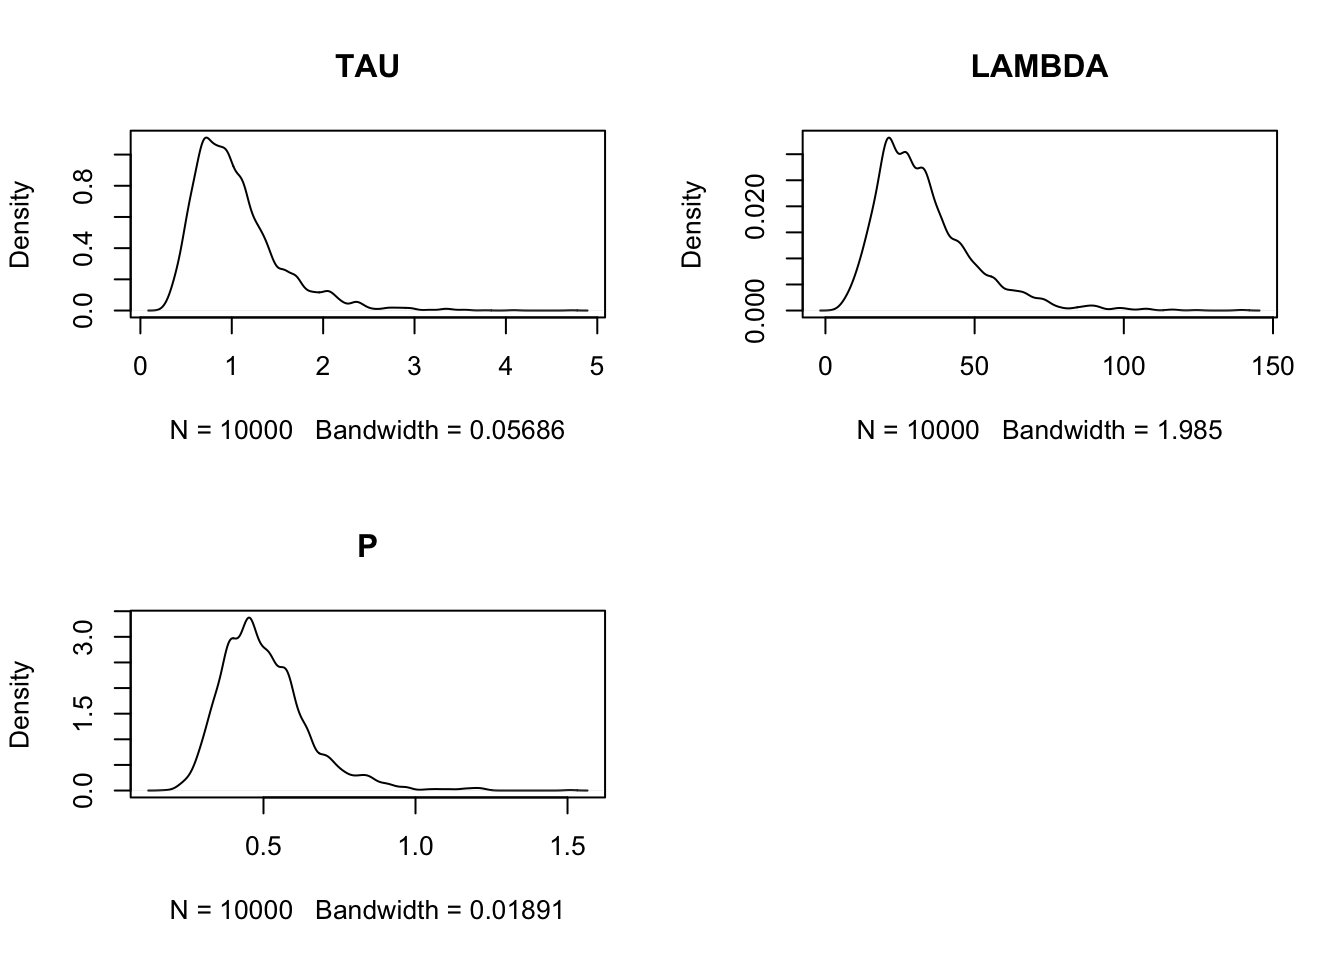
\includegraphics{bookdown-demo_files/figure-latex/unnamed-chunk-136-1.pdf}

\begin{Shaded}
\begin{Highlighting}[]
\FunctionTok{apply}\NormalTok{(}\FunctionTok{exp}\NormalTok{(s}\SpecialCharTok{$}\NormalTok{par), }\DecValTok{2}\NormalTok{, quantile, }\FunctionTok{c}\NormalTok{(.}\DecValTok{05}\NormalTok{, .}\DecValTok{5}\NormalTok{, .}\DecValTok{95}\NormalTok{))}
\end{Highlighting}
\end{Shaded}

\begin{verbatim}
##          [,1]     [,2]      [,3]
## 5%  0.4816982 13.52028 0.3185855
## 50% 0.9500635 30.09466 0.4760481
## 95% 1.8746643 65.04539 0.7455402
\end{verbatim}

\begin{Shaded}
\begin{Highlighting}[]
\FunctionTok{par}\NormalTok{(}\AttributeTok{mfrow=}\FunctionTok{c}\NormalTok{(}\DecValTok{1}\NormalTok{, }\DecValTok{1}\NormalTok{))}
\NormalTok{t }\OtherTok{\textless{}{-}} \FunctionTok{seq}\NormalTok{(}\DecValTok{1}\NormalTok{, }\DecValTok{240}\NormalTok{)}
\NormalTok{p5 }\OtherTok{\textless{}{-}} \DecValTok{0}\SpecialCharTok{*}\NormalTok{t}
\NormalTok{p50 }\OtherTok{\textless{}{-}} \DecValTok{0} \SpecialCharTok{*}\NormalTok{ t}
\NormalTok{p95 }\OtherTok{\textless{}{-}} \DecValTok{0} \SpecialCharTok{*}\NormalTok{ t}
\ControlFlowTok{for}\NormalTok{ (j }\ControlFlowTok{in} \DecValTok{1}\SpecialCharTok{:}\DecValTok{240}\NormalTok{)\{ }
\NormalTok{   S }\OtherTok{\textless{}{-}}\NormalTok{ (lambda }\SpecialCharTok{/}\NormalTok{ (lambda }\SpecialCharTok{+}\NormalTok{ t[j])) }\SpecialCharTok{\^{}}\NormalTok{ p}
\NormalTok{   q }\OtherTok{\textless{}{-}} \FunctionTok{quantile}\NormalTok{(S, }\FunctionTok{c}\NormalTok{(.}\DecValTok{05}\NormalTok{, .}\DecValTok{5}\NormalTok{, .}\DecValTok{95}\NormalTok{))}
\NormalTok{   p5[j] }\OtherTok{\textless{}{-}}\NormalTok{ q[}\DecValTok{1}\NormalTok{]}
\NormalTok{   p50[j] }\OtherTok{\textless{}{-}}\NormalTok{ q[}\DecValTok{2}\NormalTok{] }
\NormalTok{   p95[j] }\OtherTok{\textless{}{-}}\NormalTok{ q[}\DecValTok{3}\NormalTok{]}
\NormalTok{\}}
\end{Highlighting}
\end{Shaded}

Estimating a patient's survival curve.

\begin{Shaded}
\begin{Highlighting}[]
\FunctionTok{plot}\NormalTok{(t, p50, }\AttributeTok{type=}\StringTok{"l"}\NormalTok{, }
     \AttributeTok{ylim=}\FunctionTok{c}\NormalTok{(}\DecValTok{0}\NormalTok{,}\DecValTok{1}\NormalTok{), }
     \AttributeTok{ylab=}\StringTok{"Prob(Survival)"}\NormalTok{,}
     \AttributeTok{xlab=}\StringTok{"time"}\NormalTok{)}
 \FunctionTok{lines}\NormalTok{(t, p5, }\AttributeTok{lty=}\DecValTok{2}\NormalTok{)}
 \FunctionTok{lines}\NormalTok{(t, p95, }\AttributeTok{lty=}\DecValTok{2}\NormalTok{)}
\end{Highlighting}
\end{Shaded}

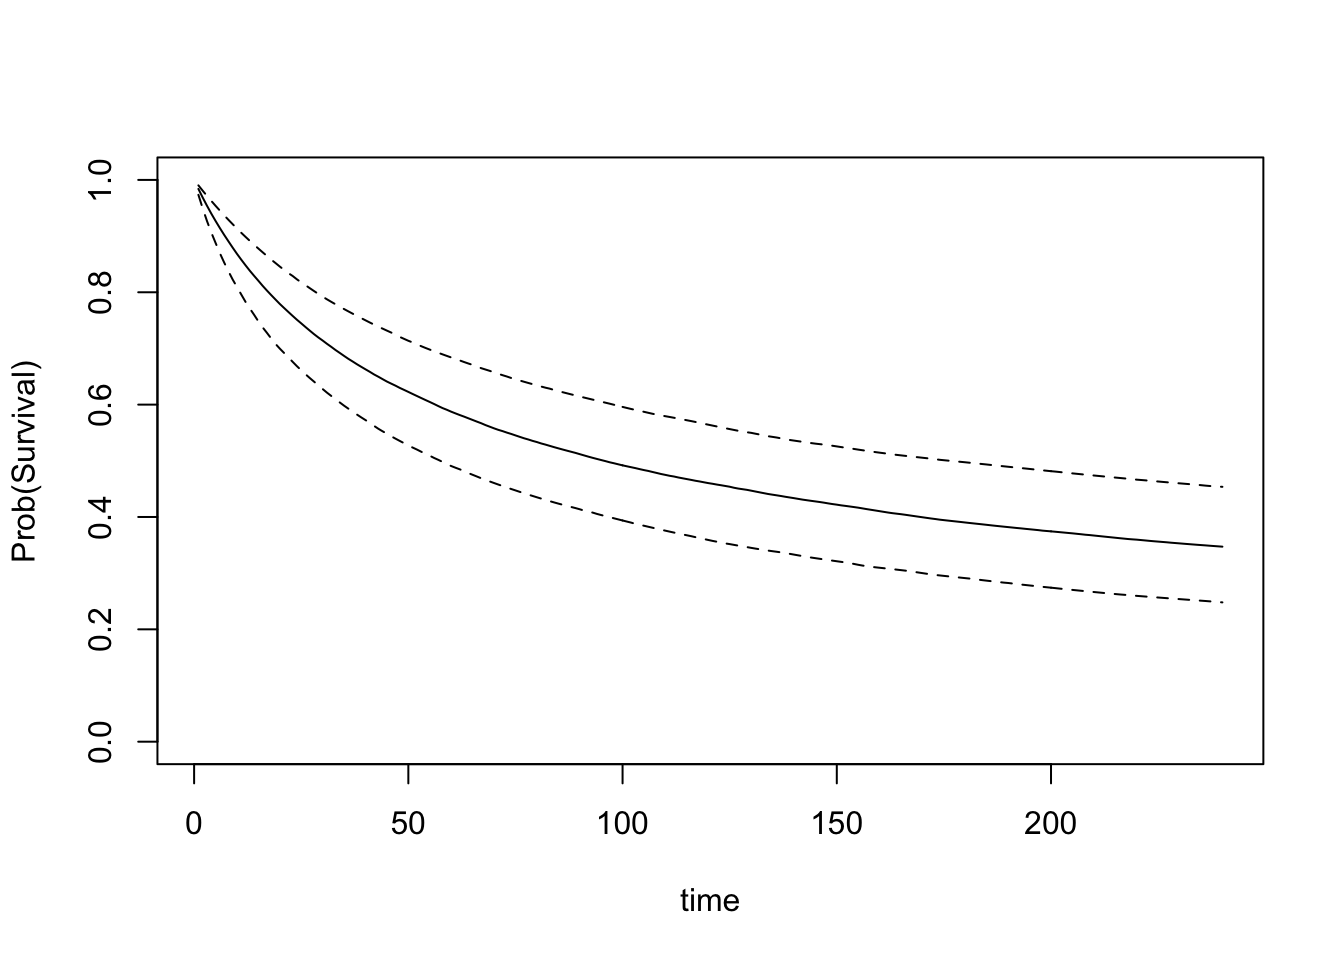
\includegraphics{bookdown-demo_files/figure-latex/unnamed-chunk-139-1.pdf}

\hypertarget{hierarchical-modeling}{%
\chapter{Hierarchical Modeling}\label{hierarchical-modeling}}

\hypertarget{introduction-to-hierarchical-modeling}{%
\section{Introduction to Hierarchical Modeling}\label{introduction-to-hierarchical-modeling}}

\begin{Shaded}
\begin{Highlighting}[]
\FunctionTok{library}\NormalTok{(LearnBayes)}
\FunctionTok{library}\NormalTok{(lattice)}
\end{Highlighting}
\end{Shaded}

Fit logistic model for home run data for a particular player

\begin{Shaded}
\begin{Highlighting}[]
\NormalTok{logistic.fit }\OtherTok{\textless{}{-}} \ControlFlowTok{function}\NormalTok{(player)\{}
\NormalTok{  d }\OtherTok{\textless{}{-}} \FunctionTok{subset}\NormalTok{(sluggerdata, Player}\SpecialCharTok{==}\NormalTok{player)}
\NormalTok{  x }\OtherTok{\textless{}{-}}\NormalTok{ d}\SpecialCharTok{$}\NormalTok{Age}
\NormalTok{  x2 }\OtherTok{\textless{}{-}}\NormalTok{ d}\SpecialCharTok{$}\NormalTok{Age}\SpecialCharTok{\^{}}\DecValTok{2}
\NormalTok{  response }\OtherTok{\textless{}{-}} \FunctionTok{cbind}\NormalTok{(d}\SpecialCharTok{$}\NormalTok{HR, d}\SpecialCharTok{$}\NormalTok{AB }\SpecialCharTok{{-}}\NormalTok{ d}\SpecialCharTok{$}\NormalTok{HR)}
  \FunctionTok{list}\NormalTok{(}\AttributeTok{Age=}\NormalTok{x,}
       \AttributeTok{p=}\FunctionTok{glm}\NormalTok{(response }\SpecialCharTok{\textasciitilde{}}\NormalTok{ x }\SpecialCharTok{+}\NormalTok{ x2,}
             \AttributeTok{family=}\NormalTok{binomial)}\SpecialCharTok{$}\NormalTok{fitted)}
\NormalTok{\}}
\end{Highlighting}
\end{Shaded}

\begin{Shaded}
\begin{Highlighting}[]
\NormalTok{names }\OtherTok{\textless{}{-}} \FunctionTok{unique}\NormalTok{(sluggerdata}\SpecialCharTok{$}\NormalTok{Player)}
\NormalTok{newdata }\OtherTok{\textless{}{-}} \ConstantTok{NULL}
\ControlFlowTok{for}\NormalTok{ (j }\ControlFlowTok{in} \DecValTok{1}\SpecialCharTok{:}\DecValTok{9}\NormalTok{)\{}
\NormalTok{  fit }\OtherTok{\textless{}{-}}\FunctionTok{logistic.fit}\NormalTok{(}\FunctionTok{as.character}\NormalTok{(names[j]))}
\NormalTok{  newdata }\OtherTok{\textless{}{-}} \FunctionTok{rbind}\NormalTok{(newdata,}
            \FunctionTok{data.frame}\NormalTok{(}\FunctionTok{as.character}\NormalTok{(names[j]),}
\NormalTok{                       fit}\SpecialCharTok{$}\NormalTok{Age, fit}\SpecialCharTok{$}\NormalTok{p))}
\NormalTok{\}}
\FunctionTok{names}\NormalTok{(newdata) }\OtherTok{\textless{}{-}} \FunctionTok{c}\NormalTok{(}\StringTok{"Player"}\NormalTok{, }\StringTok{"Age"}\NormalTok{, }\StringTok{"Fitted"}\NormalTok{)}
\FunctionTok{xyplot}\NormalTok{(Fitted }\SpecialCharTok{\textasciitilde{}}\NormalTok{ Age }\SpecialCharTok{|}\NormalTok{ Player, }
       \AttributeTok{data=}\NormalTok{newdata, }
       \AttributeTok{type=}\StringTok{"l"}\NormalTok{, }\AttributeTok{lwd=}\DecValTok{3}\NormalTok{, }\AttributeTok{col=}\StringTok{"black"}\NormalTok{)}
\end{Highlighting}
\end{Shaded}

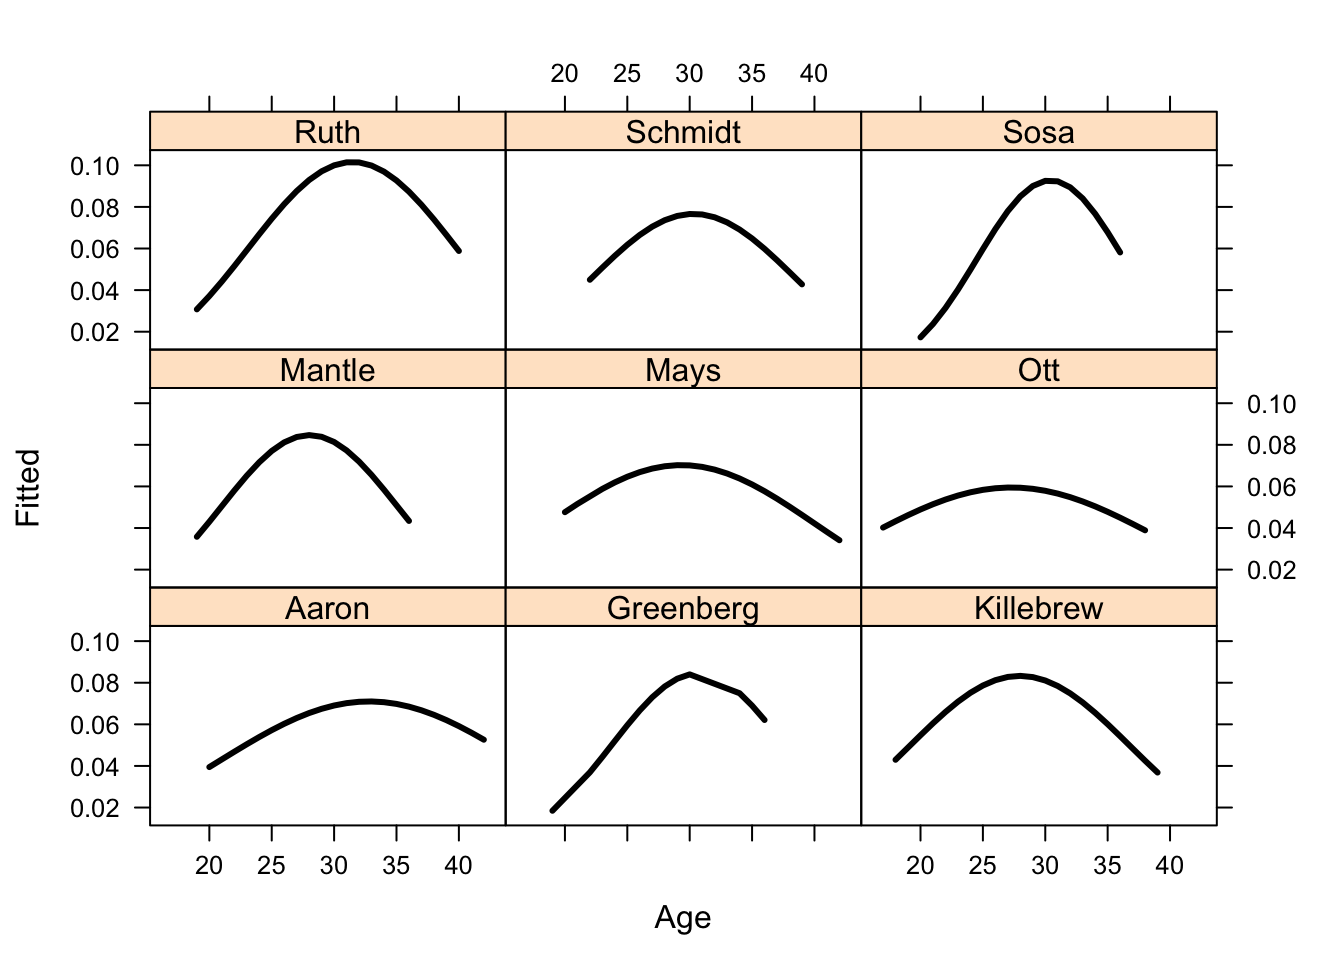
\includegraphics{bookdown-demo_files/figure-latex/unnamed-chunk-142-1.pdf}

\hypertarget{individual-or-combined-estimates}{%
\section{Individual or Combined Estimates}\label{individual-or-combined-estimates}}

\begin{Shaded}
\begin{Highlighting}[]
\FunctionTok{with}\NormalTok{(hearttransplants,}
      \FunctionTok{plot}\NormalTok{(}\FunctionTok{log}\NormalTok{(e), y }\SpecialCharTok{/}\NormalTok{ e, }\AttributeTok{xlim=}\FunctionTok{c}\NormalTok{(}\DecValTok{6}\NormalTok{, }\FloatTok{9.7}\NormalTok{),}
           \AttributeTok{xlab=}\StringTok{"log(e)"}\NormalTok{, }\AttributeTok{ylab=}\StringTok{"y/e"}\NormalTok{))}
 \FunctionTok{with}\NormalTok{(hearttransplants,}
      \FunctionTok{text}\NormalTok{(}\FunctionTok{log}\NormalTok{(e), y }\SpecialCharTok{/}\NormalTok{ e,}
           \AttributeTok{labels=}\FunctionTok{as.character}\NormalTok{(y), }\AttributeTok{pos=}\DecValTok{4}\NormalTok{))}
\end{Highlighting}
\end{Shaded}

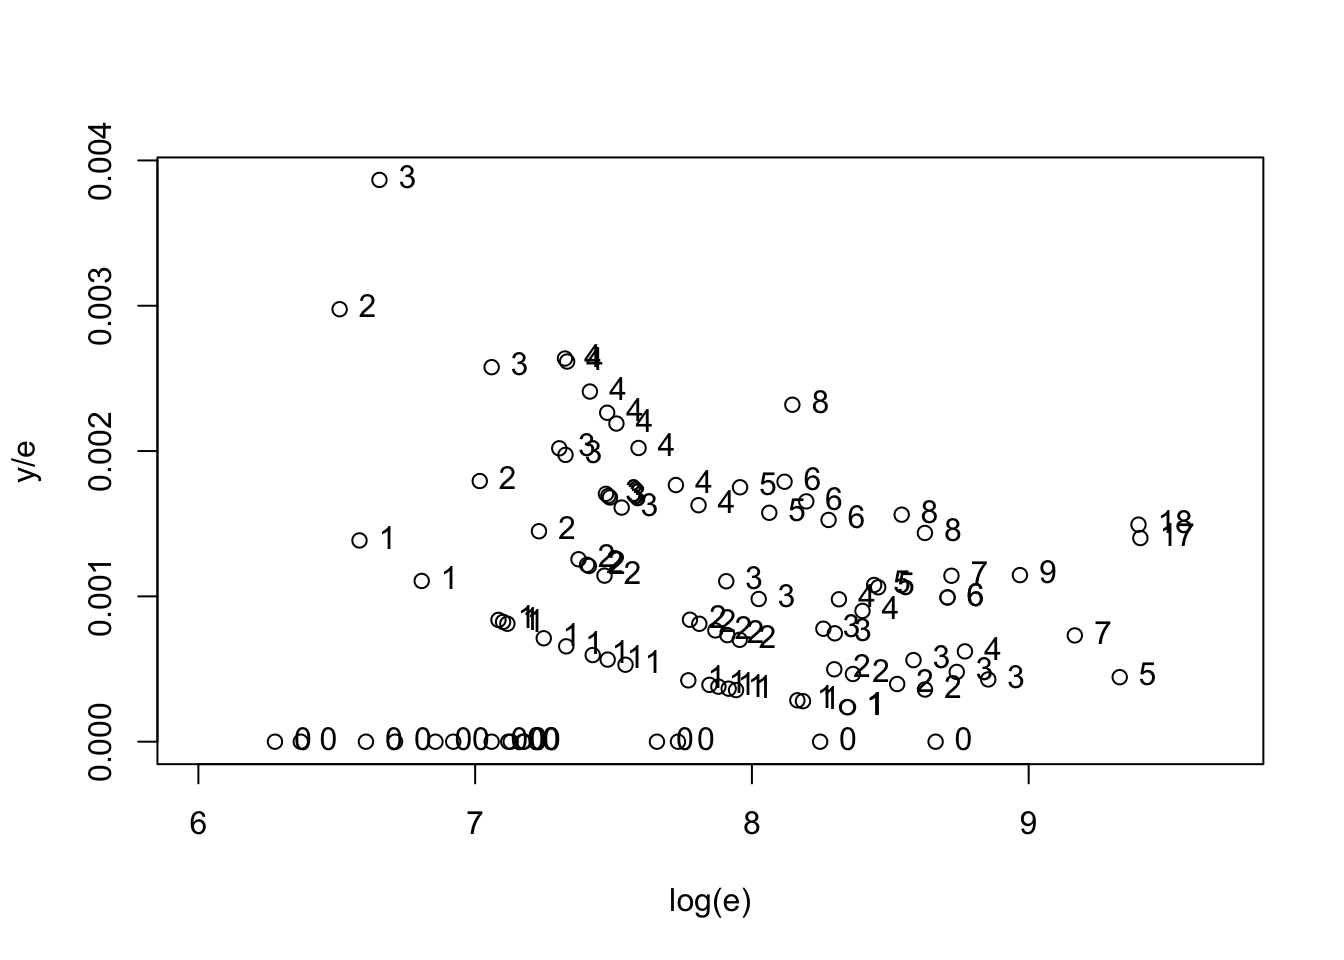
\includegraphics{bookdown-demo_files/figure-latex/unnamed-chunk-143-1.pdf}

\hypertarget{equal-mortality-rates}{%
\section{Equal Mortality Rates?}\label{equal-mortality-rates}}

Using posterior predictive checks to see if equal mortality rate model is appropriate.

\begin{Shaded}
\begin{Highlighting}[]
\FunctionTok{with}\NormalTok{(hearttransplants, }\FunctionTok{sum}\NormalTok{(y))}
\end{Highlighting}
\end{Shaded}

\begin{verbatim}
## [1] 277
\end{verbatim}

\begin{Shaded}
\begin{Highlighting}[]
\FunctionTok{with}\NormalTok{(hearttransplants, }\FunctionTok{sum}\NormalTok{(e))}
\end{Highlighting}
\end{Shaded}

\begin{verbatim}
## [1] 294681
\end{verbatim}

\begin{Shaded}
\begin{Highlighting}[]
\NormalTok{lambda }\OtherTok{\textless{}{-}} \FunctionTok{rgamma}\NormalTok{(}\DecValTok{1000}\NormalTok{, }\AttributeTok{shape=}\DecValTok{277}\NormalTok{, }\AttributeTok{rate=}\DecValTok{294681}\NormalTok{)}
\NormalTok{ys94 }\OtherTok{\textless{}{-}} \FunctionTok{with}\NormalTok{(hearttransplants,}
      \FunctionTok{rpois}\NormalTok{(}\DecValTok{1000}\NormalTok{, e[}\DecValTok{94}\NormalTok{] }\SpecialCharTok{*}\NormalTok{ lambda))}
\end{Highlighting}
\end{Shaded}

\begin{Shaded}
\begin{Highlighting}[]
\FunctionTok{hist}\NormalTok{(ys94, }\AttributeTok{breaks=}\FunctionTok{seq}\NormalTok{(}\FloatTok{0.5}\NormalTok{, }\FunctionTok{max}\NormalTok{(ys94) }\SpecialCharTok{+} \FloatTok{0.5}\NormalTok{))}
\FunctionTok{with}\NormalTok{(hearttransplants,}
      \FunctionTok{lines}\NormalTok{(}\FunctionTok{c}\NormalTok{(y[}\DecValTok{94}\NormalTok{], y[}\DecValTok{94}\NormalTok{]), }\FunctionTok{c}\NormalTok{(}\DecValTok{0}\NormalTok{, }\DecValTok{120}\NormalTok{), }\AttributeTok{lwd=}\DecValTok{3}\NormalTok{))}
\end{Highlighting}
\end{Shaded}

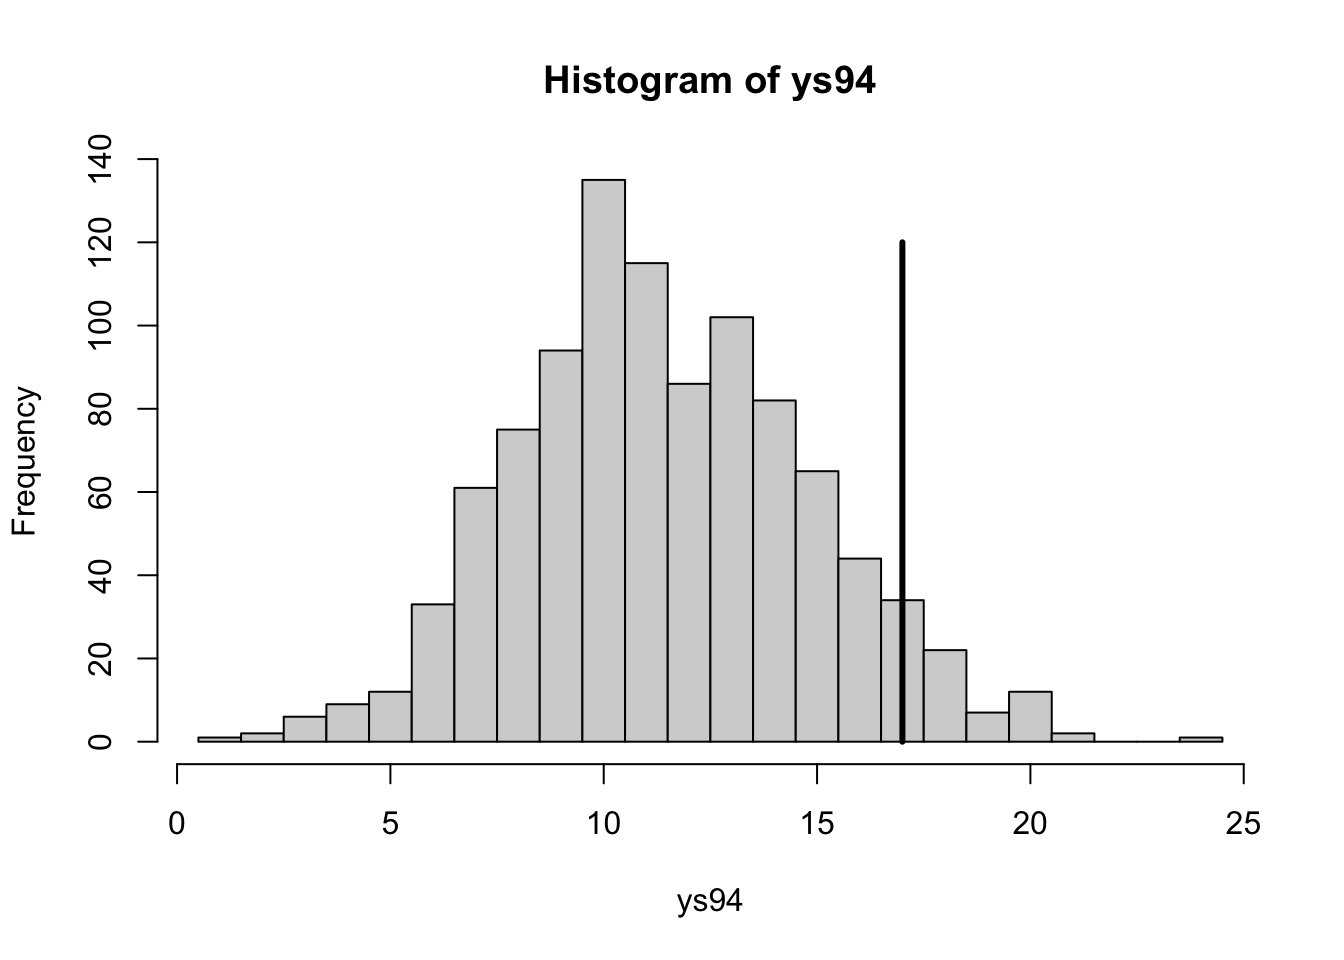
\includegraphics{bookdown-demo_files/figure-latex/unnamed-chunk-146-1.pdf}

Find posterior predictive distribution of each observation with its posterior predictive distribution.

\begin{Shaded}
\begin{Highlighting}[]
\NormalTok{lambda }\OtherTok{\textless{}{-}} \FunctionTok{rgamma}\NormalTok{(}\DecValTok{1000}\NormalTok{, }\AttributeTok{shape=}\DecValTok{277}\NormalTok{, }\AttributeTok{rate=}\DecValTok{294681}\NormalTok{)}
\NormalTok{prob.out }\OtherTok{\textless{}{-}} \ControlFlowTok{function}\NormalTok{(i)\{}
\NormalTok{   ysi }\OtherTok{\textless{}{-}} \FunctionTok{with}\NormalTok{(hearttransplants,}
            \FunctionTok{rpois}\NormalTok{(}\DecValTok{1000}\NormalTok{, e[i] }\SpecialCharTok{*}\NormalTok{ lambda))}
\NormalTok{   pleft }\OtherTok{\textless{}{-}} \FunctionTok{with}\NormalTok{(hearttransplants,}
              \FunctionTok{sum}\NormalTok{(ysi }\SpecialCharTok{\textless{}=}\NormalTok{ y[i]) }\SpecialCharTok{/} \DecValTok{1000}\NormalTok{)}
\NormalTok{   pright }\OtherTok{\textless{}{-}} \FunctionTok{with}\NormalTok{(hearttransplants,}
               \FunctionTok{sum}\NormalTok{(ysi }\SpecialCharTok{\textgreater{}=}\NormalTok{ y[i]) }\SpecialCharTok{/} \DecValTok{1000}\NormalTok{)}
   \FunctionTok{min}\NormalTok{(pleft, pright)}
\NormalTok{ \}}
\NormalTok{pout }\OtherTok{\textless{}{-}} \FunctionTok{sapply}\NormalTok{(}\DecValTok{1}\SpecialCharTok{:}\DecValTok{94}\NormalTok{, prob.out)}
\end{Highlighting}
\end{Shaded}

\begin{Shaded}
\begin{Highlighting}[]
\FunctionTok{with}\NormalTok{(hearttransplants,}
     \FunctionTok{plot}\NormalTok{(}\FunctionTok{log}\NormalTok{(e), pout, }\AttributeTok{ylab=}\StringTok{"Prob(extreme)"}\NormalTok{))}
\end{Highlighting}
\end{Shaded}

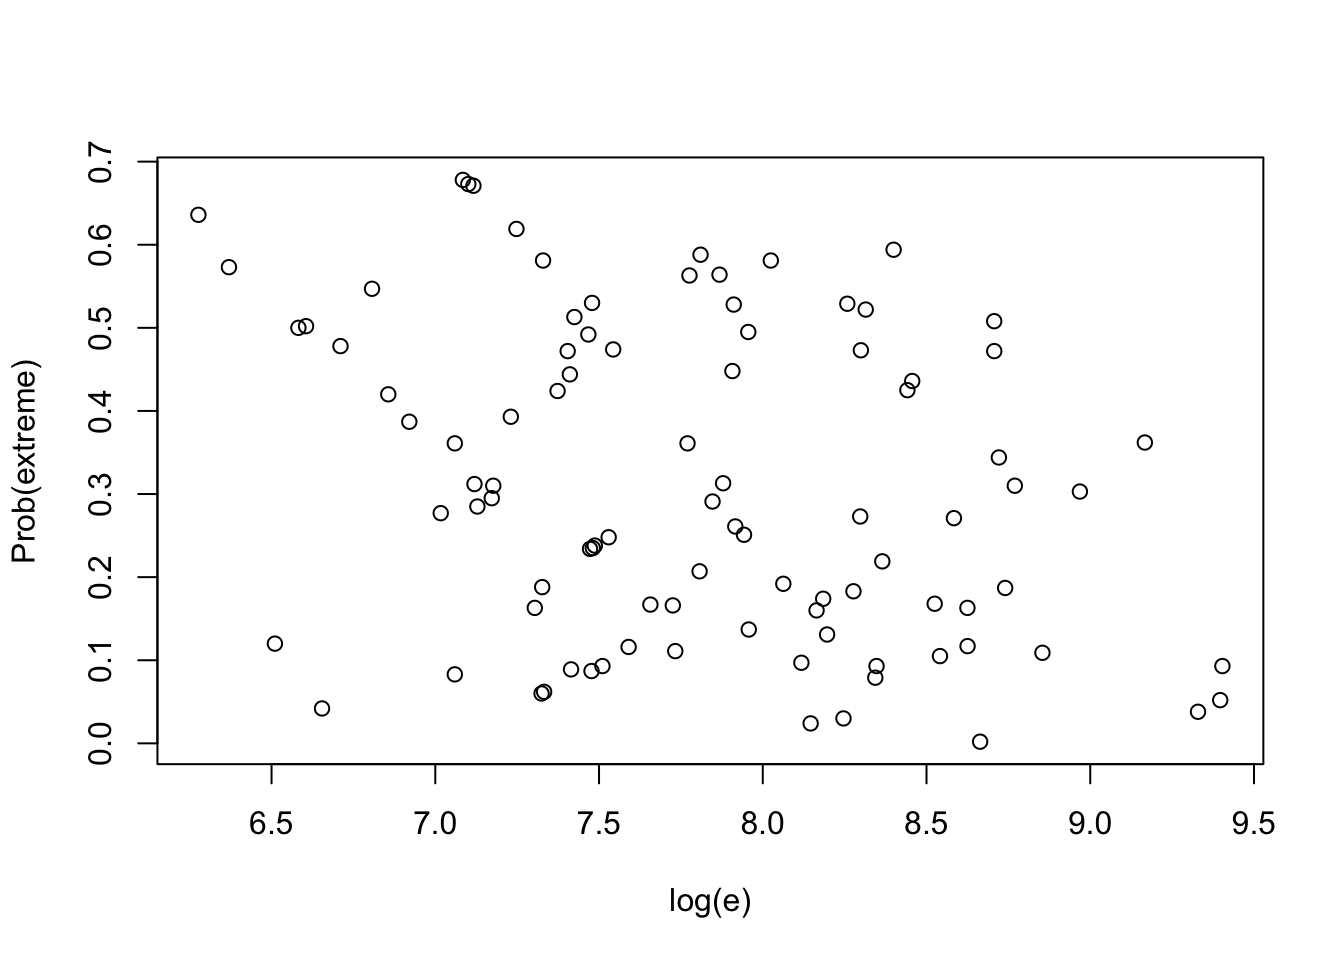
\includegraphics{bookdown-demo_files/figure-latex/unnamed-chunk-148-1.pdf}

\hypertarget{modeling-a-prior-belief-of-exchangeability}{%
\section{Modeling a Prior Belief of Exchangeability}\label{modeling-a-prior-belief-of-exchangeability}}

Graph of two-stage prior to model a belief in exchangeability of the Poisson rates.

\begin{Shaded}
\begin{Highlighting}[]
\NormalTok{pgexchprior }\OtherTok{\textless{}{-}} \ControlFlowTok{function}\NormalTok{(lambda, pars)\{}
\NormalTok{alpha }\OtherTok{\textless{}{-}}\NormalTok{ pars[}\DecValTok{1}\NormalTok{]}
\NormalTok{a }\OtherTok{\textless{}{-}}\NormalTok{ pars[}\DecValTok{2}\NormalTok{]}
\NormalTok{b }\OtherTok{\textless{}{-}}\NormalTok{ pars[}\DecValTok{3}\NormalTok{]}
\NormalTok{(alpha }\SpecialCharTok{{-}} \DecValTok{1}\NormalTok{) }\SpecialCharTok{*} \FunctionTok{log}\NormalTok{(}\FunctionTok{prod}\NormalTok{(lambda)) }\SpecialCharTok{{-}} 
\NormalTok{  (}\DecValTok{2} \SpecialCharTok{*}\NormalTok{ alpha }\SpecialCharTok{+}\NormalTok{ a) }\SpecialCharTok{*} \FunctionTok{log}\NormalTok{(alpha }\SpecialCharTok{*} \FunctionTok{sum}\NormalTok{(lambda) }\SpecialCharTok{+}\NormalTok{ b)}
\NormalTok{\}}
\end{Highlighting}
\end{Shaded}

\begin{Shaded}
\begin{Highlighting}[]
\NormalTok{alpha }\OtherTok{\textless{}{-}} \FunctionTok{c}\NormalTok{(}\DecValTok{5}\NormalTok{, }\DecValTok{20}\NormalTok{, }\DecValTok{80}\NormalTok{, }\DecValTok{400}\NormalTok{)}
\FunctionTok{par}\NormalTok{(}\AttributeTok{mfrow=}\FunctionTok{c}\NormalTok{(}\DecValTok{2}\NormalTok{, }\DecValTok{2}\NormalTok{))}
\ControlFlowTok{for}\NormalTok{ (j }\ControlFlowTok{in} \DecValTok{1}\SpecialCharTok{:}\DecValTok{4}\NormalTok{)\{}
    \FunctionTok{mycontour}\NormalTok{(pgexchprior,}
              \FunctionTok{c}\NormalTok{(.}\DecValTok{001}\NormalTok{, }\DecValTok{5}\NormalTok{, .}\DecValTok{001}\NormalTok{, }\DecValTok{5}\NormalTok{),}
              \FunctionTok{c}\NormalTok{(alpha[j], }\DecValTok{10}\NormalTok{, }\DecValTok{10}\NormalTok{),}
          \AttributeTok{main=}\FunctionTok{paste}\NormalTok{(}\StringTok{"ALPHA = "}\NormalTok{,alpha[j]),}
         \AttributeTok{xlab=}\StringTok{"LAMBDA 1"}\NormalTok{, }\AttributeTok{ylab=}\StringTok{"LAMBDA 2"}\NormalTok{)}
\NormalTok{\}}
\end{Highlighting}
\end{Shaded}

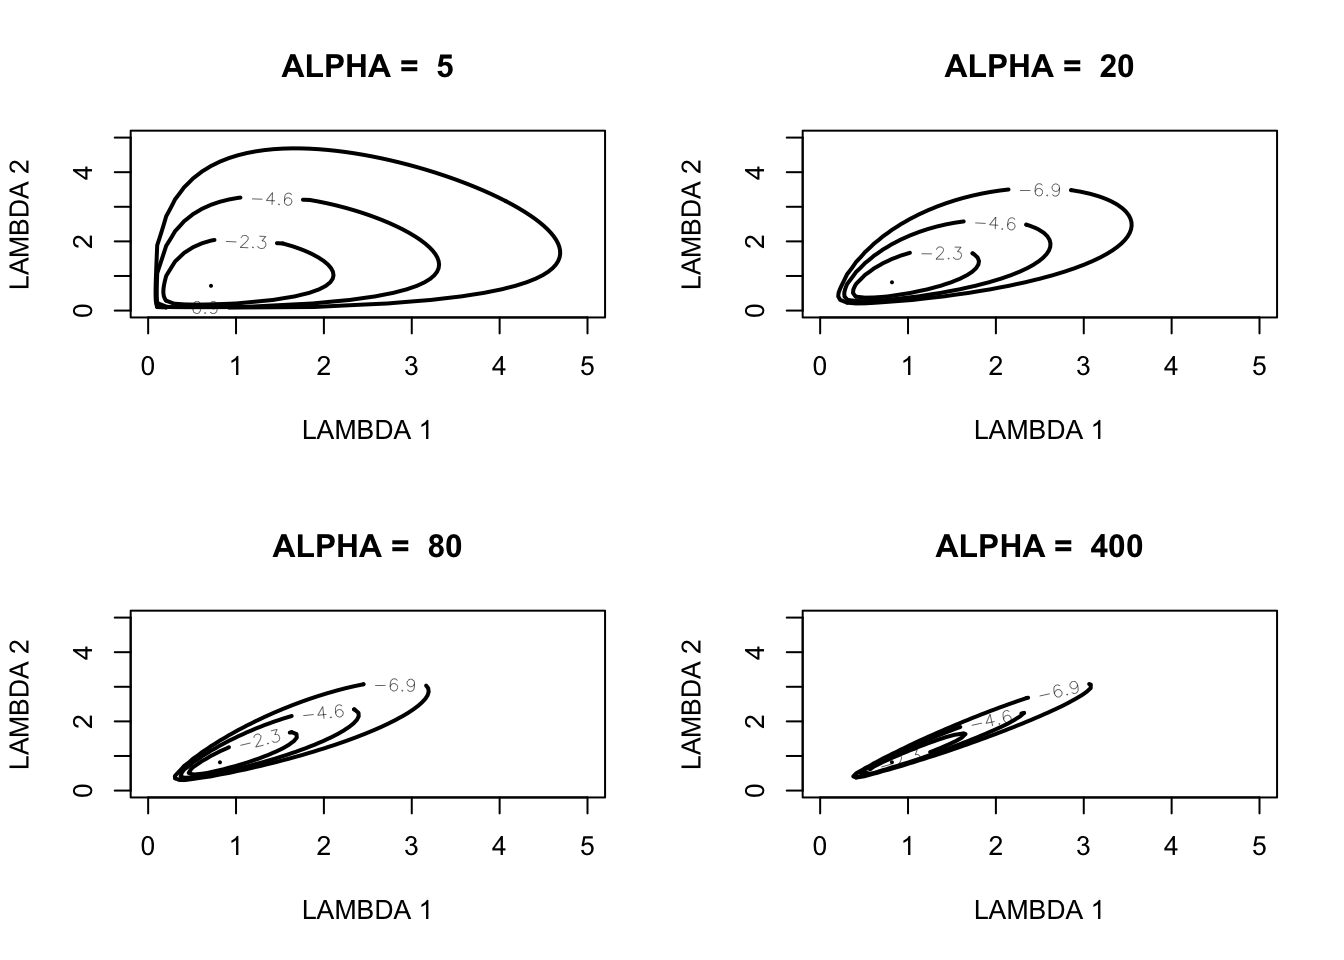
\includegraphics{bookdown-demo_files/figure-latex/unnamed-chunk-150-1.pdf}

\hypertarget{simulating-from-the-posterior}{%
\section{Simulating from the Posterior}\label{simulating-from-the-posterior}}

Representing posterior as {[}\(\mu, \alpha\){]} {[}\(\{\lambda_j\} | \mu, \alpha\){]}.

Focus on posterior of {[}\(\mu, \alpha\){]}:

\begin{Shaded}
\begin{Highlighting}[]
\NormalTok{datapar }\OtherTok{\textless{}{-}} \FunctionTok{list}\NormalTok{(}\AttributeTok{data =}\NormalTok{ hearttransplants, }\AttributeTok{z0 =} \FloatTok{0.53}\NormalTok{)}
\NormalTok{start }\OtherTok{\textless{}{-}} \FunctionTok{c}\NormalTok{(}\DecValTok{2}\NormalTok{, }\SpecialCharTok{{-}}\DecValTok{7}\NormalTok{)}
\NormalTok{fit }\OtherTok{\textless{}{-}} \FunctionTok{laplace}\NormalTok{(poissgamexch, start, datapar)}
\NormalTok{ fit}
\end{Highlighting}
\end{Shaded}

\begin{verbatim}
## $mode
## [1]  1.883954 -6.955446
## 
## $var
##              [,1]         [,2]
## [1,]  0.233694921 -0.003086655
## [2,] -0.003086655  0.005866020
## 
## $int
## [1] -2208.503
## 
## $converge
## [1] TRUE
\end{verbatim}

\begin{Shaded}
\begin{Highlighting}[]
\FunctionTok{par}\NormalTok{(}\AttributeTok{mfrow =} \FunctionTok{c}\NormalTok{(}\DecValTok{1}\NormalTok{, }\DecValTok{1}\NormalTok{))}
\FunctionTok{mycontour}\NormalTok{(poissgamexch, }\FunctionTok{c}\NormalTok{(}\DecValTok{0}\NormalTok{, }\DecValTok{8}\NormalTok{, }\SpecialCharTok{{-}}\FloatTok{7.3}\NormalTok{, }\SpecialCharTok{{-}}\FloatTok{6.6}\NormalTok{),}
\NormalTok{          datapar,}
          \AttributeTok{xlab=}\StringTok{"log alpha"}\NormalTok{, }\AttributeTok{ylab=}\StringTok{"log mu"}\NormalTok{)}
\end{Highlighting}
\end{Shaded}

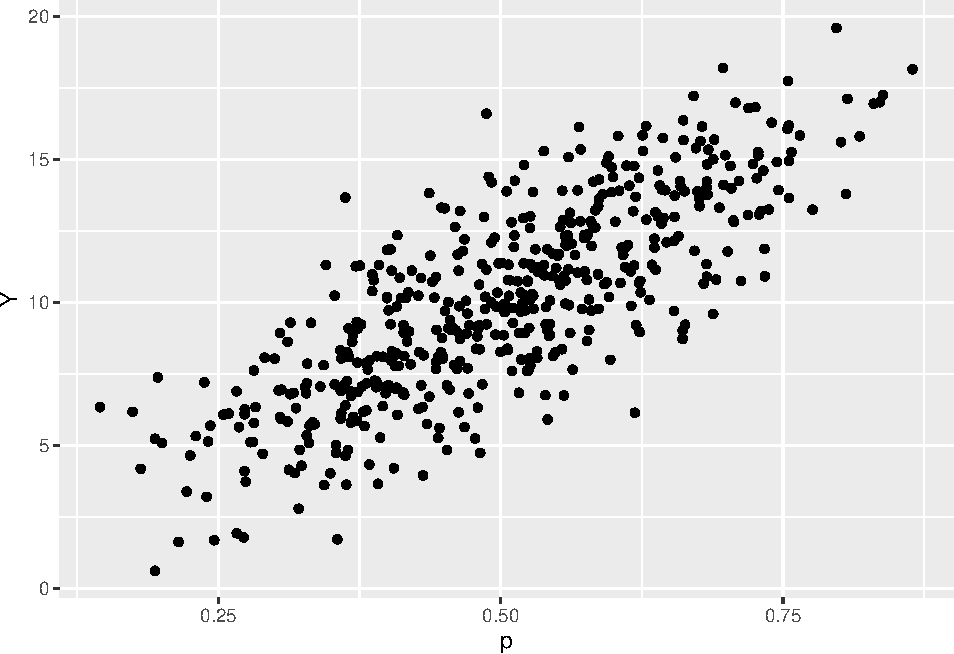
\includegraphics{bookdown-demo_files/figure-latex/unnamed-chunk-152-1.pdf}

\begin{Shaded}
\begin{Highlighting}[]
\NormalTok{start }\OtherTok{\textless{}{-}} \FunctionTok{c}\NormalTok{(}\DecValTok{4}\NormalTok{, }\SpecialCharTok{{-}}\DecValTok{7}\NormalTok{)}
\NormalTok{fitgibbs }\OtherTok{\textless{}{-}} \FunctionTok{gibbs}\NormalTok{(poissgamexch, }
\NormalTok{                  start, }\DecValTok{1000}\NormalTok{, }
                  \FunctionTok{c}\NormalTok{(}\DecValTok{1}\NormalTok{, .}\DecValTok{15}\NormalTok{), datapar)}
\NormalTok{fitgibbs}\SpecialCharTok{$}\NormalTok{accept}
\end{Highlighting}
\end{Shaded}

\begin{verbatim}
##       [,1]  [,2]
## [1,] 0.502 0.476
\end{verbatim}

\begin{Shaded}
\begin{Highlighting}[]
\FunctionTok{mycontour}\NormalTok{(poissgamexch, }
         \FunctionTok{c}\NormalTok{(}\DecValTok{0}\NormalTok{, }\DecValTok{8}\NormalTok{, }\SpecialCharTok{{-}}\FloatTok{7.3}\NormalTok{, }\SpecialCharTok{{-}}\FloatTok{6.6}\NormalTok{), }
\NormalTok{         datapar,}
         \AttributeTok{xlab=}\StringTok{"log alpha"}\NormalTok{, }\AttributeTok{ylab=}\StringTok{"log mu"}\NormalTok{)}
\FunctionTok{points}\NormalTok{(fitgibbs}\SpecialCharTok{$}\NormalTok{par[, }\DecValTok{1}\NormalTok{], fitgibbs}\SpecialCharTok{$}\NormalTok{par[, }\DecValTok{2}\NormalTok{])}
\end{Highlighting}
\end{Shaded}

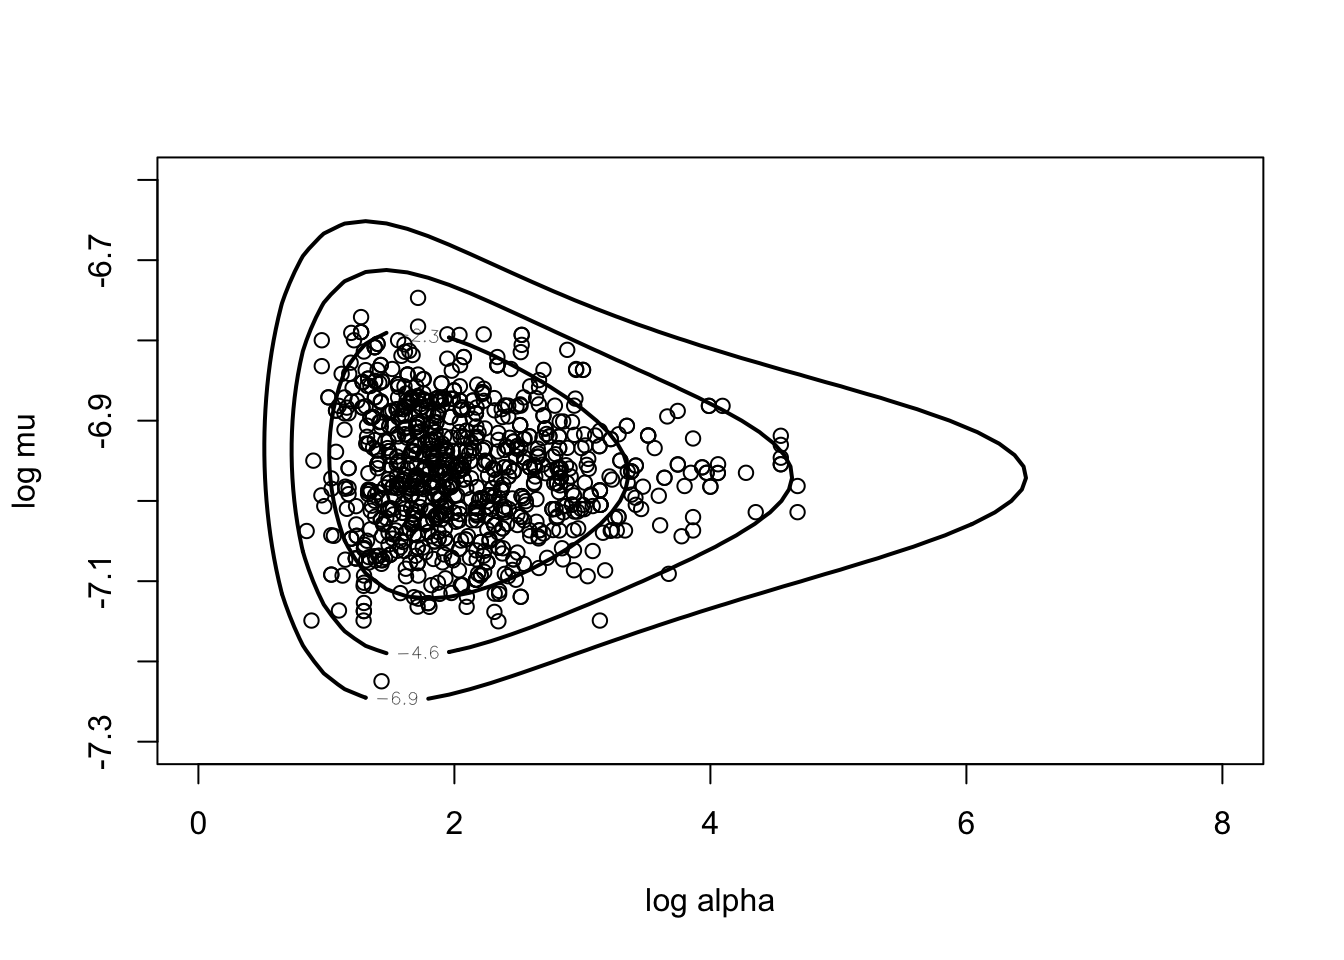
\includegraphics{bookdown-demo_files/figure-latex/unnamed-chunk-154-1.pdf}

\begin{Shaded}
\begin{Highlighting}[]
\FunctionTok{plot}\NormalTok{(}\FunctionTok{density}\NormalTok{(fitgibbs}\SpecialCharTok{$}\NormalTok{par[, }\DecValTok{1}\NormalTok{], }\AttributeTok{bw =} \FloatTok{0.2}\NormalTok{))}
\end{Highlighting}
\end{Shaded}

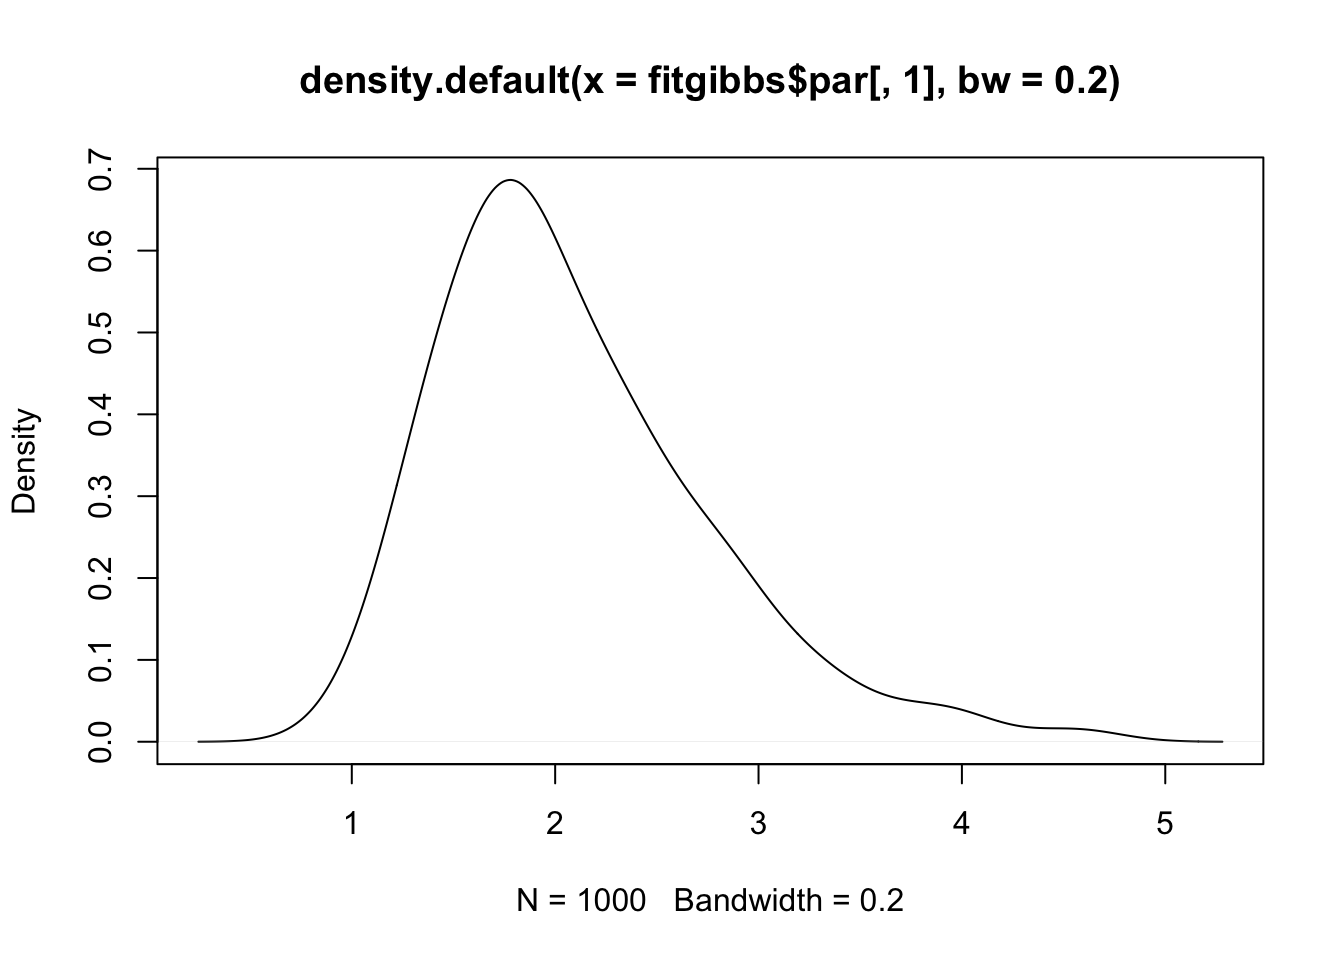
\includegraphics{bookdown-demo_files/figure-latex/unnamed-chunk-155-1.pdf}

Posterior of rates:

\begin{Shaded}
\begin{Highlighting}[]
\NormalTok{alpha }\OtherTok{\textless{}{-}} \FunctionTok{exp}\NormalTok{(fitgibbs}\SpecialCharTok{$}\NormalTok{par[, }\DecValTok{1}\NormalTok{])}
\NormalTok{mu }\OtherTok{\textless{}{-}} \FunctionTok{exp}\NormalTok{(fitgibbs}\SpecialCharTok{$}\NormalTok{par[, }\DecValTok{2}\NormalTok{])}
\NormalTok{lam1 }\OtherTok{\textless{}{-}} \FunctionTok{rgamma}\NormalTok{(}\DecValTok{1000}\NormalTok{, y[}\DecValTok{1}\NormalTok{] }\SpecialCharTok{+}\NormalTok{ alpha, }
\NormalTok{               hearttransplants}\SpecialCharTok{$}\NormalTok{e[}\DecValTok{1}\NormalTok{] }\SpecialCharTok{+}\NormalTok{ alpha }\SpecialCharTok{/}\NormalTok{ mu)}
\NormalTok{alpha }\OtherTok{\textless{}{-}} \FunctionTok{exp}\NormalTok{(fitgibbs}\SpecialCharTok{$}\NormalTok{par[, }\DecValTok{1}\NormalTok{])}
\NormalTok{mu }\OtherTok{\textless{}{-}} \FunctionTok{exp}\NormalTok{(fitgibbs}\SpecialCharTok{$}\NormalTok{par[, }\DecValTok{2}\NormalTok{])}
\end{Highlighting}
\end{Shaded}

\begin{Shaded}
\begin{Highlighting}[]
\FunctionTok{with}\NormalTok{(hearttransplants,}
     \FunctionTok{plot}\NormalTok{(}\FunctionTok{log}\NormalTok{(e), y}\SpecialCharTok{/}\NormalTok{e, }\AttributeTok{pch =} \FunctionTok{as.character}\NormalTok{(y)))}
 \ControlFlowTok{for}\NormalTok{ (i }\ControlFlowTok{in} \DecValTok{1}\SpecialCharTok{:}\DecValTok{94}\NormalTok{) \{}
\NormalTok{     lami }\OtherTok{\textless{}{-}} \FunctionTok{with}\NormalTok{(hearttransplants,}
           \FunctionTok{rgamma}\NormalTok{(}\DecValTok{1000}\NormalTok{, y[i] }\SpecialCharTok{+}\NormalTok{ alpha, }
\NormalTok{               e[i] }\SpecialCharTok{+}\NormalTok{ alpha}\SpecialCharTok{/}\NormalTok{mu))}
\NormalTok{     probint }\OtherTok{\textless{}{-}} \FunctionTok{quantile}\NormalTok{(lami, }\FunctionTok{c}\NormalTok{(}\FloatTok{0.05}\NormalTok{, }\FloatTok{0.95}\NormalTok{))}
     \FunctionTok{with}\NormalTok{(hearttransplants,}
          \FunctionTok{lines}\NormalTok{(}\FunctionTok{log}\NormalTok{(e[i]) }\SpecialCharTok{*} \FunctionTok{c}\NormalTok{(}\DecValTok{1}\NormalTok{, }\DecValTok{1}\NormalTok{), probint))}
\NormalTok{ \}}
\end{Highlighting}
\end{Shaded}

\includegraphics{bookdown-demo_files/figure-latex/unnamed-chunk-157-1.pdf}

\hypertarget{posterior-inferences}{%
\section{Posterior Inferences}\label{posterior-inferences}}

\begin{Shaded}
\begin{Highlighting}[]
\NormalTok{datapar }\OtherTok{\textless{}{-}} \FunctionTok{list}\NormalTok{(}\AttributeTok{data =}\NormalTok{ hearttransplants, }\AttributeTok{z0 =} \FloatTok{0.53}\NormalTok{)}
\NormalTok{start }\OtherTok{\textless{}{-}} \FunctionTok{c}\NormalTok{(}\DecValTok{2}\NormalTok{, }\SpecialCharTok{{-}}\DecValTok{7}\NormalTok{)}
\NormalTok{fit }\OtherTok{\textless{}{-}} \FunctionTok{laplace}\NormalTok{(poissgamexch, start, datapar)}
\NormalTok{fit}
\end{Highlighting}
\end{Shaded}

\begin{verbatim}
## $mode
## [1]  1.883954 -6.955446
## 
## $var
##              [,1]         [,2]
## [1,]  0.233694921 -0.003086655
## [2,] -0.003086655  0.005866020
## 
## $int
## [1] -2208.503
## 
## $converge
## [1] TRUE
\end{verbatim}

\begin{Shaded}
\begin{Highlighting}[]
\FunctionTok{par}\NormalTok{(}\AttributeTok{mfrow =} \FunctionTok{c}\NormalTok{(}\DecValTok{1}\NormalTok{, }\DecValTok{1}\NormalTok{))}
\FunctionTok{mycontour}\NormalTok{(poissgamexch, }
          \FunctionTok{c}\NormalTok{(}\DecValTok{0}\NormalTok{, }\DecValTok{8}\NormalTok{, }\SpecialCharTok{{-}}\FloatTok{7.3}\NormalTok{, }\SpecialCharTok{{-}}\FloatTok{6.6}\NormalTok{), datapar,}
          \AttributeTok{xlab=}\StringTok{"log alpha"}\NormalTok{,}\AttributeTok{ylab=}\StringTok{"log mu"}\NormalTok{)}
\end{Highlighting}
\end{Shaded}

\includegraphics{bookdown-demo_files/figure-latex/unnamed-chunk-159-1.pdf}

\begin{Shaded}
\begin{Highlighting}[]
\NormalTok{start }\OtherTok{\textless{}{-}} \FunctionTok{c}\NormalTok{(}\DecValTok{4}\NormalTok{, }\SpecialCharTok{{-}}\DecValTok{7}\NormalTok{)}
\NormalTok{fitgibbs }\OtherTok{\textless{}{-}} \FunctionTok{gibbs}\NormalTok{(poissgamexch, }
\NormalTok{                  start, }\DecValTok{1000}\NormalTok{, }
                  \FunctionTok{c}\NormalTok{(}\DecValTok{1}\NormalTok{,.}\DecValTok{15}\NormalTok{), datapar)}
\end{Highlighting}
\end{Shaded}

\begin{Shaded}
\begin{Highlighting}[]
\NormalTok{alpha }\OtherTok{\textless{}{-}} \FunctionTok{exp}\NormalTok{(fitgibbs}\SpecialCharTok{$}\NormalTok{par[, }\DecValTok{1}\NormalTok{])}
\NormalTok{mu }\OtherTok{\textless{}{-}} \FunctionTok{exp}\NormalTok{(fitgibbs}\SpecialCharTok{$}\NormalTok{par[, }\DecValTok{2}\NormalTok{])}
\end{Highlighting}
\end{Shaded}

Look at posteriors of shrinkages.

\begin{Shaded}
\begin{Highlighting}[]
\NormalTok{shrink }\OtherTok{\textless{}{-}}\ControlFlowTok{function}\NormalTok{(i)}
\FunctionTok{with}\NormalTok{(hearttransplants,}
       \FunctionTok{mean}\NormalTok{(alpha }\SpecialCharTok{/}\NormalTok{ (alpha }\SpecialCharTok{+}\NormalTok{ e[i] }\SpecialCharTok{*}\NormalTok{ mu)))}
\NormalTok{shrinkage}\OtherTok{=}\FunctionTok{sapply}\NormalTok{(}\DecValTok{1}\SpecialCharTok{:}\DecValTok{94}\NormalTok{, shrink)}
\end{Highlighting}
\end{Shaded}

\begin{Shaded}
\begin{Highlighting}[]
\FunctionTok{with}\NormalTok{(hearttransplants,}
     \FunctionTok{plot}\NormalTok{(}\FunctionTok{log}\NormalTok{(e), shrinkage))}
\end{Highlighting}
\end{Shaded}

\includegraphics{bookdown-demo_files/figure-latex/unnamed-chunk-163-1.pdf}

Comparing hospitals.

\begin{Shaded}
\begin{Highlighting}[]
\NormalTok{mrate }\OtherTok{\textless{}{-}} \ControlFlowTok{function}\NormalTok{(i)\{}
   \FunctionTok{with}\NormalTok{(hearttransplants,}
       \FunctionTok{mean}\NormalTok{(}\FunctionTok{rgamma}\NormalTok{(}\DecValTok{1000}\NormalTok{, y[i] }\SpecialCharTok{+}\NormalTok{ alpha, }
\NormalTok{                  e[i] }\SpecialCharTok{+}\NormalTok{ alpha}\SpecialCharTok{/}\NormalTok{mu)))}
\NormalTok{\}}
\NormalTok{hospital }\OtherTok{\textless{}{-}} \DecValTok{1}\SpecialCharTok{:}\DecValTok{94}
\NormalTok{meanrate }\OtherTok{\textless{}{-}} \FunctionTok{sapply}\NormalTok{(hospital,mrate)}
\NormalTok{hospital[meanrate }\SpecialCharTok{==} \FunctionTok{min}\NormalTok{(meanrate)]}
\end{Highlighting}
\end{Shaded}

\begin{verbatim}
## [1] 85
\end{verbatim}

\begin{Shaded}
\begin{Highlighting}[]
\NormalTok{sim.lambda }\OtherTok{\textless{}{-}} \ControlFlowTok{function}\NormalTok{(i) \{}
  \FunctionTok{with}\NormalTok{(hearttransplants,}
       \FunctionTok{rgamma}\NormalTok{(}\DecValTok{1000}\NormalTok{, y[i] }\SpecialCharTok{+}\NormalTok{ alpha, }
\NormalTok{              e[i] }\SpecialCharTok{+}\NormalTok{ alpha }\SpecialCharTok{/}\NormalTok{ mu))}
\NormalTok{\}}
\NormalTok{LAM }\OtherTok{\textless{}{-}} \FunctionTok{sapply}\NormalTok{(}\DecValTok{1}\SpecialCharTok{:}\DecValTok{94}\NormalTok{, sim.lambda)}
\end{Highlighting}
\end{Shaded}

\begin{Shaded}
\begin{Highlighting}[]
\NormalTok{compare.rates }\OtherTok{\textless{}{-}} \ControlFlowTok{function}\NormalTok{(x) \{}
\NormalTok{  nc }\OtherTok{\textless{}{-}} \FunctionTok{NCOL}\NormalTok{(x)}
\NormalTok{  ij }\OtherTok{\textless{}{-}} \FunctionTok{as.matrix}\NormalTok{(}\FunctionTok{expand.grid}\NormalTok{(}\DecValTok{1}\SpecialCharTok{:}\NormalTok{nc, }\DecValTok{1}\SpecialCharTok{:}\NormalTok{nc))}
\NormalTok{  m }\OtherTok{\textless{}{-}} \FunctionTok{as.matrix}\NormalTok{(x[,ij[,}\DecValTok{1}\NormalTok{]] }\SpecialCharTok{\textgreater{}}\NormalTok{ x[,ij[,}\DecValTok{2}\NormalTok{]])}
  \FunctionTok{matrix}\NormalTok{(}\FunctionTok{colMeans}\NormalTok{(m), nc, nc, }\AttributeTok{byrow =} \ConstantTok{TRUE}\NormalTok{)}
\NormalTok{\}}
\end{Highlighting}
\end{Shaded}

\begin{Shaded}
\begin{Highlighting}[]
\NormalTok{better }\OtherTok{\textless{}{-}} \FunctionTok{compare.rates}\NormalTok{(LAM)}
\end{Highlighting}
\end{Shaded}

\begin{Shaded}
\begin{Highlighting}[]
\NormalTok{better[}\DecValTok{1}\SpecialCharTok{:}\DecValTok{24}\NormalTok{, }\DecValTok{85}\NormalTok{]}
\end{Highlighting}
\end{Shaded}

\begin{verbatim}
##  [1] 0.195 0.197 0.095 0.124 0.141 0.231 0.214 0.168 0.079 0.198 0.197 0.162
## [13] 0.198 0.098 0.069 0.209 0.231 0.095 0.265 0.153 0.140 0.154 0.051 0.067
\end{verbatim}

\hypertarget{bayesian-sensitivity-analysis}{%
\section{Bayesian Sensitivity Analysis}\label{bayesian-sensitivity-analysis}}

Explore sensitivity of inference with respect to the choice of \(z_0\) in prior.

\begin{Shaded}
\begin{Highlighting}[]
\NormalTok{datapar }\OtherTok{\textless{}{-}} \FunctionTok{list}\NormalTok{(}\AttributeTok{data =}\NormalTok{ hearttransplants, }
                \AttributeTok{z0 =} \FloatTok{0.53}\NormalTok{)}
\end{Highlighting}
\end{Shaded}

\begin{Shaded}
\begin{Highlighting}[]
\NormalTok{start }\OtherTok{\textless{}{-}} \FunctionTok{c}\NormalTok{(}\DecValTok{4}\NormalTok{, }\SpecialCharTok{{-}}\DecValTok{7}\NormalTok{)}
\NormalTok{fitgibbs }\OtherTok{\textless{}{-}}\FunctionTok{gibbs}\NormalTok{(poissgamexch, }
\NormalTok{                 start, }\DecValTok{1000}\NormalTok{, }
                 \FunctionTok{c}\NormalTok{(}\DecValTok{1}\NormalTok{,.}\DecValTok{15}\NormalTok{), datapar)}
\end{Highlighting}
\end{Shaded}

\begin{Shaded}
\begin{Highlighting}[]
\NormalTok{sir.old.new }\OtherTok{\textless{}{-}} \ControlFlowTok{function}\NormalTok{(theta, prior, prior.new)\{}
\NormalTok{  log.g }\OtherTok{\textless{}{-}} \FunctionTok{log}\NormalTok{(}\FunctionTok{prior}\NormalTok{(theta))}
\NormalTok{  log.g.new }\OtherTok{\textless{}{-}} \FunctionTok{log}\NormalTok{(}\FunctionTok{prior.new}\NormalTok{(theta))}
\NormalTok{  wt }\OtherTok{\textless{}{-}} \FunctionTok{exp}\NormalTok{(log.g.new }\SpecialCharTok{{-}}\NormalTok{ log.g }\SpecialCharTok{{-}}
              \FunctionTok{max}\NormalTok{(log.g.new }\SpecialCharTok{{-}}\NormalTok{ log.g))}
\NormalTok{  probs }\OtherTok{\textless{}{-}}\NormalTok{ wt }\SpecialCharTok{/} \FunctionTok{sum}\NormalTok{(wt)}
\NormalTok{  n }\OtherTok{\textless{}{-}} \FunctionTok{length}\NormalTok{(probs)}
\NormalTok{  indices }\OtherTok{\textless{}{-}} \FunctionTok{sample}\NormalTok{(}\DecValTok{1}\SpecialCharTok{:}\NormalTok{n, }\AttributeTok{size=}\NormalTok{n, }
                    \AttributeTok{prob=}\NormalTok{probs, }\AttributeTok{replace=}\ConstantTok{TRUE}\NormalTok{)}
\NormalTok{  theta[indices]}
\NormalTok{\}}
\end{Highlighting}
\end{Shaded}

\begin{Shaded}
\begin{Highlighting}[]
\NormalTok{prior }\OtherTok{\textless{}{-}} \ControlFlowTok{function}\NormalTok{(theta)\{}
  \FloatTok{0.53} \SpecialCharTok{*} \FunctionTok{exp}\NormalTok{(theta) }\SpecialCharTok{/}\NormalTok{ (}\FunctionTok{exp}\NormalTok{(theta) }\SpecialCharTok{+} \FloatTok{0.53}\NormalTok{) }\SpecialCharTok{\^{}} \DecValTok{2}
\NormalTok{\}}
\NormalTok{prior.new }\OtherTok{\textless{}{-}} \ControlFlowTok{function}\NormalTok{(theta)\{}
  \DecValTok{5} \SpecialCharTok{*} \FunctionTok{exp}\NormalTok{(theta) }\SpecialCharTok{/}\NormalTok{ (}\FunctionTok{exp}\NormalTok{(theta) }\SpecialCharTok{+} \DecValTok{5}\NormalTok{) }\SpecialCharTok{\^{}} \DecValTok{2}
\NormalTok{\}}
\end{Highlighting}
\end{Shaded}

\begin{Shaded}
\begin{Highlighting}[]
\NormalTok{log.alpha }\OtherTok{\textless{}{-}}\NormalTok{ fitgibbs}\SpecialCharTok{$}\NormalTok{par[, }\DecValTok{1}\NormalTok{]}
\NormalTok{log.alpha.new }\OtherTok{\textless{}{-}} \FunctionTok{sir.old.new}\NormalTok{(log.alpha, }
\NormalTok{                             prior, prior.new)}
\end{Highlighting}
\end{Shaded}

\begin{Shaded}
\begin{Highlighting}[]
\FunctionTok{library}\NormalTok{(lattice)}
\end{Highlighting}
\end{Shaded}

\begin{Shaded}
\begin{Highlighting}[]
\NormalTok{draw.graph }\OtherTok{\textless{}{-}} \ControlFlowTok{function}\NormalTok{()\{}
\NormalTok{  LOG.ALPHA }\OtherTok{\textless{}{-}} \FunctionTok{data.frame}\NormalTok{(}\StringTok{"prior"}\NormalTok{, log.alpha)}
  \FunctionTok{names}\NormalTok{(LOG.ALPHA) }\OtherTok{\textless{}{-}} \FunctionTok{c}\NormalTok{(}\StringTok{"Prior"}\NormalTok{, }\StringTok{"log.alpha"}\NormalTok{)}
\NormalTok{  LOG.ALPHA.NEW }\OtherTok{\textless{}{-}} \FunctionTok{data.frame}\NormalTok{(}\StringTok{"new.prior"}\NormalTok{,}
\NormalTok{                              log.alpha.new)}
  \FunctionTok{names}\NormalTok{(LOG.ALPHA.NEW) }\OtherTok{\textless{}{-}} \FunctionTok{c}\NormalTok{(}\StringTok{"Prior"}\NormalTok{,}\StringTok{"log.alpha"}\NormalTok{)}
\NormalTok{  D }\OtherTok{\textless{}{-}} \FunctionTok{densityplot}\NormalTok{(}\SpecialCharTok{\textasciitilde{}}\NormalTok{ log.alpha,}
            \AttributeTok{group=}\NormalTok{Prior,}
            \AttributeTok{data =} \FunctionTok{rbind}\NormalTok{(LOG.ALPHA, LOG.ALPHA.NEW),}
            \AttributeTok{plot.points=}\ConstantTok{FALSE}\NormalTok{,}
        \AttributeTok{main=}\StringTok{"Original Prior and Posterior (solid), }\SpecialCharTok{\textbackslash{}n}\StringTok{New Prior and Posterior (dashed)"}\NormalTok{,}
        \AttributeTok{lwd=}\DecValTok{4}\NormalTok{, }\AttributeTok{adjust=}\DecValTok{2}\NormalTok{, }\AttributeTok{lty=}\FunctionTok{c}\NormalTok{(}\DecValTok{1}\NormalTok{,}\DecValTok{2}\NormalTok{),}
        \AttributeTok{xlab=}\StringTok{"log alpha"}\NormalTok{,}\AttributeTok{xlim=}\FunctionTok{c}\NormalTok{(}\SpecialCharTok{{-}}\DecValTok{3}\NormalTok{,}\DecValTok{5}\NormalTok{),}\AttributeTok{col=}\StringTok{"black"}\NormalTok{)}
    \FunctionTok{update}\NormalTok{(D, }\AttributeTok{panel=}\ControlFlowTok{function}\NormalTok{(...)\{}
      \FunctionTok{panel.curve}\NormalTok{(}\FunctionTok{prior}\NormalTok{(x), }\AttributeTok{lty=}\DecValTok{1}\NormalTok{, }\AttributeTok{lwd=}\DecValTok{2}\NormalTok{,}
                  \AttributeTok{col=}\StringTok{"black"}\NormalTok{)}
      \FunctionTok{panel.curve}\NormalTok{(}\FunctionTok{prior.new}\NormalTok{(x), }\AttributeTok{lty=}\DecValTok{2}\NormalTok{, }\AttributeTok{lwd=}\DecValTok{2}\NormalTok{,}
                  \AttributeTok{col=}\StringTok{"black"}\NormalTok{)}
    \FunctionTok{panel.densityplot}\NormalTok{(...)}
\NormalTok{\})\}}
\end{Highlighting}
\end{Shaded}

\begin{Shaded}
\begin{Highlighting}[]
\FunctionTok{draw.graph}\NormalTok{()}
\end{Highlighting}
\end{Shaded}

\includegraphics{bookdown-demo_files/figure-latex/unnamed-chunk-176-1.pdf}

\hypertarget{posterior-predictive-model-checking}{%
\section{Posterior Predictive Model Checking}\label{posterior-predictive-model-checking}}

Study predictive distributions of observations.

\begin{Shaded}
\begin{Highlighting}[]
\NormalTok{datapar }\OtherTok{\textless{}{-}} \FunctionTok{list}\NormalTok{(}\AttributeTok{data =}\NormalTok{ hearttransplants, }\AttributeTok{z0 =} \FloatTok{0.53}\NormalTok{)}
\end{Highlighting}
\end{Shaded}

\begin{Shaded}
\begin{Highlighting}[]
\NormalTok{start }\OtherTok{\textless{}{-}} \FunctionTok{c}\NormalTok{(}\DecValTok{4}\NormalTok{, }\SpecialCharTok{{-}}\DecValTok{7}\NormalTok{)}
\NormalTok{fitgibbs }\OtherTok{\textless{}{-}} \FunctionTok{gibbs}\NormalTok{(poissgamexch, }
\NormalTok{                  start, }\DecValTok{1000}\NormalTok{, }\FunctionTok{c}\NormalTok{(}\DecValTok{1}\NormalTok{,.}\DecValTok{15}\NormalTok{), }
\NormalTok{                  datapar)}
\end{Highlighting}
\end{Shaded}

\begin{Shaded}
\begin{Highlighting}[]
\NormalTok{lam94 }\OtherTok{\textless{}{-}} \FunctionTok{with}\NormalTok{(hearttransplants,}
      \FunctionTok{rgamma}\NormalTok{(}\DecValTok{1000}\NormalTok{, y[}\DecValTok{94}\NormalTok{] }\SpecialCharTok{+}\NormalTok{ alpha, }
\NormalTok{             e[}\DecValTok{94}\NormalTok{] }\SpecialCharTok{+}\NormalTok{ alpha }\SpecialCharTok{/}\NormalTok{ mu))}
\end{Highlighting}
\end{Shaded}

\begin{Shaded}
\begin{Highlighting}[]
\NormalTok{ys94 }\OtherTok{\textless{}{-}} \FunctionTok{with}\NormalTok{(hearttransplants,}
           \FunctionTok{rpois}\NormalTok{(}\DecValTok{1000}\NormalTok{, e[}\DecValTok{94}\NormalTok{] }\SpecialCharTok{*}\NormalTok{ lam94))}
\end{Highlighting}
\end{Shaded}

\begin{Shaded}
\begin{Highlighting}[]
\FunctionTok{hist}\NormalTok{(ys94, }\AttributeTok{breaks=}\FunctionTok{seq}\NormalTok{(}\SpecialCharTok{{-}}\FloatTok{0.5}\NormalTok{, }\FunctionTok{max}\NormalTok{(ys94) }\SpecialCharTok{+} \FloatTok{0.5}\NormalTok{))}
\FunctionTok{lines}\NormalTok{(y[}\DecValTok{94}\NormalTok{] }\SpecialCharTok{*} \FunctionTok{c}\NormalTok{(}\DecValTok{1}\NormalTok{, }\DecValTok{1}\NormalTok{), }\FunctionTok{c}\NormalTok{(}\DecValTok{0}\NormalTok{, }\DecValTok{100}\NormalTok{), }\AttributeTok{lwd=}\DecValTok{3}\NormalTok{)}
\end{Highlighting}
\end{Shaded}

\includegraphics{bookdown-demo_files/figure-latex/unnamed-chunk-181-1.pdf}

Explore the probabilities that the predictive distribution of each observation is at least as large as observed \(y_i\).

\begin{Shaded}
\begin{Highlighting}[]
\NormalTok{prob.out }\OtherTok{\textless{}{-}} \ControlFlowTok{function}\NormalTok{(i)\{}
\NormalTok{   lami }\OtherTok{\textless{}{-}} \FunctionTok{with}\NormalTok{(hearttransplants,}
      \FunctionTok{rgamma}\NormalTok{(}\DecValTok{1000}\NormalTok{, y[i] }\SpecialCharTok{+}\NormalTok{ alpha, }
\NormalTok{             e[i] }\SpecialCharTok{+}\NormalTok{ alpha }\SpecialCharTok{/}\NormalTok{ mu))}
\NormalTok{   ysi }\OtherTok{\textless{}{-}} \FunctionTok{with}\NormalTok{(hearttransplants,}
      \FunctionTok{rpois}\NormalTok{(}\DecValTok{1000}\NormalTok{, e[i] }\SpecialCharTok{*}\NormalTok{ lami))}
\NormalTok{   pleft }\OtherTok{\textless{}{-}} \FunctionTok{with}\NormalTok{(hearttransplants,}
      \FunctionTok{sum}\NormalTok{(ysi }\SpecialCharTok{\textless{}=}\NormalTok{ y[i]) }\SpecialCharTok{/} \DecValTok{1000}\NormalTok{)}
\NormalTok{   pright }\OtherTok{\textless{}{-}} \FunctionTok{with}\NormalTok{(hearttransplants,}
      \FunctionTok{sum}\NormalTok{(ysi }\SpecialCharTok{\textgreater{}=}\NormalTok{ y[i]) }\SpecialCharTok{/} \DecValTok{1000}\NormalTok{)}
   \FunctionTok{min}\NormalTok{(pleft, pright)}
\NormalTok{ \}}
\NormalTok{pout.exchange }\OtherTok{\textless{}{-}} \FunctionTok{sapply}\NormalTok{(}\DecValTok{1}\SpecialCharTok{:}\DecValTok{94}\NormalTok{, prob.out)}
\end{Highlighting}
\end{Shaded}

\begin{Shaded}
\begin{Highlighting}[]
\FunctionTok{plot}\NormalTok{(pout, pout.exchange,}
     \AttributeTok{xlab=}\StringTok{"P(extreme), equal means"}\NormalTok{,}
     \AttributeTok{ylab=}\StringTok{"P(extreme), exchangeable"}\NormalTok{)}
\FunctionTok{abline}\NormalTok{(}\DecValTok{0}\NormalTok{,}\DecValTok{1}\NormalTok{)}
\end{Highlighting}
\end{Shaded}

\includegraphics{bookdown-demo_files/figure-latex/unnamed-chunk-183-1.pdf}

\hypertarget{model-comparison}{%
\chapter{Model Comparison}\label{model-comparison}}

\hypertarget{a-one-sided-test-of-a-normal-mean}{%
\section{A One-Sided Test of a Normal Mean}\label{a-one-sided-test-of-a-normal-mean}}

Bayesian testing of \(\mu \le \mu_0\) against \(\mu > \mu_0\).

\begin{Shaded}
\begin{Highlighting}[]
\FunctionTok{library}\NormalTok{(LearnBayes)}
\end{Highlighting}
\end{Shaded}

\begin{Shaded}
\begin{Highlighting}[]
\NormalTok{pmean }\OtherTok{\textless{}{-}} \DecValTok{170}
\NormalTok{pvar }\OtherTok{\textless{}{-}} \DecValTok{25}
\NormalTok{probH }\OtherTok{\textless{}{-}} \FunctionTok{pnorm}\NormalTok{(}\DecValTok{175}\NormalTok{, pmean, }\FunctionTok{sqrt}\NormalTok{(pvar))}
\NormalTok{probA }\OtherTok{\textless{}{-}} \DecValTok{1} \SpecialCharTok{{-}}\NormalTok{ probH}
\NormalTok{prior.odds }\OtherTok{\textless{}{-}}\NormalTok{ probH }\SpecialCharTok{/}\NormalTok{ probA}
\NormalTok{prior.odds}
\end{Highlighting}
\end{Shaded}

\begin{verbatim}
## [1] 5.302974
\end{verbatim}

\begin{Shaded}
\begin{Highlighting}[]
\NormalTok{weights }\OtherTok{\textless{}{-}} \FunctionTok{c}\NormalTok{(}\DecValTok{182}\NormalTok{, }\DecValTok{172}\NormalTok{, }\DecValTok{173}\NormalTok{, }\DecValTok{176}\NormalTok{, }\DecValTok{176}\NormalTok{, }\DecValTok{180}\NormalTok{,}
             \DecValTok{173}\NormalTok{, }\DecValTok{174}\NormalTok{, }\DecValTok{179}\NormalTok{, }\DecValTok{175}\NormalTok{)}
\NormalTok{xbar }\OtherTok{\textless{}{-}} \FunctionTok{mean}\NormalTok{(weights)}
\NormalTok{sigma2 }\OtherTok{\textless{}{-}} \DecValTok{3} \SpecialCharTok{\^{}} \DecValTok{2} \SpecialCharTok{/} \FunctionTok{length}\NormalTok{(weights)}
\end{Highlighting}
\end{Shaded}

\begin{Shaded}
\begin{Highlighting}[]
\NormalTok{post.precision }\OtherTok{\textless{}{-}} \DecValTok{1} \SpecialCharTok{/}\NormalTok{ sigma2 }\SpecialCharTok{+} \DecValTok{1} \SpecialCharTok{/}\NormalTok{ pvar}
\NormalTok{post.var }\OtherTok{\textless{}{-}} \DecValTok{1} \SpecialCharTok{/}\NormalTok{ post.precision}
\end{Highlighting}
\end{Shaded}

\begin{Shaded}
\begin{Highlighting}[]
\NormalTok{post.mean }\OtherTok{\textless{}{-}}\NormalTok{ (xbar }\SpecialCharTok{/}\NormalTok{ sigma2 }\SpecialCharTok{+}\NormalTok{ pmean }\SpecialCharTok{/}\NormalTok{ pvar) }\SpecialCharTok{/} 
\NormalTok{          post.precision}
\FunctionTok{c}\NormalTok{(post.mean, }\FunctionTok{sqrt}\NormalTok{(post.var))}
\end{Highlighting}
\end{Shaded}

\begin{verbatim}
## [1] 175.7915058   0.9320546
\end{verbatim}

\begin{Shaded}
\begin{Highlighting}[]
\NormalTok{post.odds }\OtherTok{\textless{}{-}} \FunctionTok{pnorm}\NormalTok{(}\DecValTok{175}\NormalTok{, post.mean, }
                   \FunctionTok{sqrt}\NormalTok{(post.var)) }\SpecialCharTok{/}
\NormalTok{           (}\DecValTok{1} \SpecialCharTok{{-}} \FunctionTok{pnorm}\NormalTok{(}\DecValTok{175}\NormalTok{, post.mean,}
                   \FunctionTok{sqrt}\NormalTok{(post.var)))}
\NormalTok{post.odds}
\end{Highlighting}
\end{Shaded}

\begin{verbatim}
## [1] 0.2467017
\end{verbatim}

\begin{Shaded}
\begin{Highlighting}[]
\NormalTok{BF }\OtherTok{\textless{}{-}}\NormalTok{ post.odds }\SpecialCharTok{/}\NormalTok{ prior.odds}
\NormalTok{BF}
\end{Highlighting}
\end{Shaded}

\begin{verbatim}
## [1] 0.04652139
\end{verbatim}

\begin{Shaded}
\begin{Highlighting}[]
\NormalTok{postH  }\OtherTok{\textless{}{-}}\NormalTok{ probH }\SpecialCharTok{*}\NormalTok{ BF }\SpecialCharTok{/}\NormalTok{ (probH }\SpecialCharTok{*}\NormalTok{ BF }\SpecialCharTok{+}\NormalTok{ probA)}
\NormalTok{postH}
\end{Highlighting}
\end{Shaded}

\begin{verbatim}
## [1] 0.1978835
\end{verbatim}

Contrast with a frequentist p-value calculation.

\begin{Shaded}
\begin{Highlighting}[]
\NormalTok{z }\OtherTok{\textless{}{-}} \FunctionTok{sqrt}\NormalTok{(}\FunctionTok{length}\NormalTok{(weights)) }\SpecialCharTok{*} 
\NormalTok{  (}\FunctionTok{mean}\NormalTok{(weights) }\SpecialCharTok{{-}} \DecValTok{175}\NormalTok{) }\SpecialCharTok{/} \DecValTok{3}
\DecValTok{1} \SpecialCharTok{{-}} \FunctionTok{pnorm}\NormalTok{(z)}
\end{Highlighting}
\end{Shaded}

\begin{verbatim}
## [1] 0.1459203
\end{verbatim}

\begin{Shaded}
\begin{Highlighting}[]
\NormalTok{weights }\OtherTok{\textless{}{-}} \FunctionTok{c}\NormalTok{(}\DecValTok{182}\NormalTok{, }\DecValTok{172}\NormalTok{, }\DecValTok{173}\NormalTok{, }\DecValTok{176}\NormalTok{, }\DecValTok{176}\NormalTok{, }\DecValTok{180}\NormalTok{,}
          \DecValTok{173}\NormalTok{, }\DecValTok{174}\NormalTok{, }\DecValTok{179}\NormalTok{, }\DecValTok{175}\NormalTok{)}
\NormalTok{data }\OtherTok{\textless{}{-}} \FunctionTok{c}\NormalTok{(}\FunctionTok{mean}\NormalTok{(weights), }\FunctionTok{length}\NormalTok{(weights), }\DecValTok{3}\NormalTok{)}
\NormalTok{prior.par }\OtherTok{\textless{}{-}} \FunctionTok{c}\NormalTok{(}\DecValTok{170}\NormalTok{, }\DecValTok{1000}\NormalTok{)}
\FunctionTok{mnormt.onesided}\NormalTok{(}\DecValTok{175}\NormalTok{, prior.par, data)}
\end{Highlighting}
\end{Shaded}

\begin{verbatim}
## $BF
## [1] 0.1694947
## 
## $prior.odds
## [1] 1.008011
## 
## $post.odds
## [1] 0.1708525
## 
## $postH
## [1] 0.1459215
\end{verbatim}

\hypertarget{a-two-sided-test-of-a-normal-mean}{%
\section{A Two-Sided Test of a Normal Mean}\label{a-two-sided-test-of-a-normal-mean}}

Bayesian testing of \(\mu = \mu_0\) against \(\mu \neq \mu_0\).

\begin{Shaded}
\begin{Highlighting}[]
\NormalTok{weights }\OtherTok{\textless{}{-}} \FunctionTok{c}\NormalTok{(}\DecValTok{182}\NormalTok{, }\DecValTok{172}\NormalTok{, }\DecValTok{173}\NormalTok{, }\DecValTok{176}\NormalTok{, }\DecValTok{176}\NormalTok{, }\DecValTok{180}\NormalTok{,}
             \DecValTok{173}\NormalTok{, }\DecValTok{174}\NormalTok{, }\DecValTok{179}\NormalTok{, }\DecValTok{175}\NormalTok{)}
\end{Highlighting}
\end{Shaded}

\begin{Shaded}
\begin{Highlighting}[]
\NormalTok{data }\OtherTok{\textless{}{-}} \FunctionTok{c}\NormalTok{(}\FunctionTok{mean}\NormalTok{(weights), }\FunctionTok{length}\NormalTok{(weights), }\DecValTok{3}\NormalTok{)}
\NormalTok{t }\OtherTok{\textless{}{-}} \FunctionTok{c}\NormalTok{(.}\DecValTok{5}\NormalTok{, }\DecValTok{1}\NormalTok{, }\DecValTok{2}\NormalTok{, }\DecValTok{4}\NormalTok{, }\DecValTok{8}\NormalTok{)}
\FunctionTok{mnormt.twosided}\NormalTok{(}\DecValTok{170}\NormalTok{, .}\DecValTok{5}\NormalTok{, t, data)}
\end{Highlighting}
\end{Shaded}

\begin{verbatim}
## $bf
## [1] 1.462146e-02 3.897038e-05 1.894326e-07 2.591162e-08 2.309739e-08
## 
## $post
## [1] 1.441076e-02 3.896887e-05 1.894325e-07 2.591162e-08 2.309739e-08
\end{verbatim}

\hypertarget{models-for-soccer-goals}{%
\section{Models for Soccer Goals}\label{models-for-soccer-goals}}

Illustrates the use of the marginal likelihood to compare several Bayesian models for soccer goals.

\begin{Shaded}
\begin{Highlighting}[]
\NormalTok{datapar }\OtherTok{\textless{}{-}} \FunctionTok{list}\NormalTok{(}\AttributeTok{data=}\NormalTok{soccergoals}\SpecialCharTok{$}\NormalTok{goals,}
                \AttributeTok{par=}\FunctionTok{c}\NormalTok{(}\FloatTok{4.57}\NormalTok{, }\FloatTok{1.43}\NormalTok{))}
\NormalTok{fit1 }\OtherTok{\textless{}{-}} \FunctionTok{laplace}\NormalTok{(logpoissgamma, .}\DecValTok{5}\NormalTok{, datapar)}
\NormalTok{datapar }\OtherTok{\textless{}{-}} \FunctionTok{list}\NormalTok{(}\AttributeTok{data=}\NormalTok{soccergoals}\SpecialCharTok{$}\NormalTok{goals,}
                \AttributeTok{par=}\FunctionTok{c}\NormalTok{(}\DecValTok{1}\NormalTok{, .}\DecValTok{5}\NormalTok{))}
\NormalTok{fit2 }\OtherTok{\textless{}{-}} \FunctionTok{laplace}\NormalTok{(logpoissnormal, .}\DecValTok{5}\NormalTok{, datapar)}
\NormalTok{datapar }\OtherTok{\textless{}{-}} \FunctionTok{list}\NormalTok{(}\AttributeTok{data=}\NormalTok{soccergoals}\SpecialCharTok{$}\NormalTok{goals,}
                \AttributeTok{par=}\FunctionTok{c}\NormalTok{(}\DecValTok{2}\NormalTok{, .}\DecValTok{5}\NormalTok{))}
\NormalTok{fit3 }\OtherTok{\textless{}{-}} \FunctionTok{laplace}\NormalTok{(logpoissnormal, .}\DecValTok{5}\NormalTok{, datapar)}
\NormalTok{datapar }\OtherTok{\textless{}{-}} \FunctionTok{list}\NormalTok{(}\AttributeTok{data=}\NormalTok{soccergoals}\SpecialCharTok{$}\NormalTok{goals,}
                \AttributeTok{par=}\FunctionTok{c}\NormalTok{(}\DecValTok{1}\NormalTok{, }\DecValTok{2}\NormalTok{))}
\NormalTok{fit4 }\OtherTok{\textless{}{-}} \FunctionTok{laplace}\NormalTok{(logpoissnormal, .}\DecValTok{5}\NormalTok{, datapar)}
\end{Highlighting}
\end{Shaded}

\begin{Shaded}
\begin{Highlighting}[]
\NormalTok{postmode }\OtherTok{\textless{}{-}} \FunctionTok{c}\NormalTok{(fit1}\SpecialCharTok{$}\NormalTok{mode, fit2}\SpecialCharTok{$}\NormalTok{mode, fit3}\SpecialCharTok{$}\NormalTok{mode,}
\NormalTok{              fit4}\SpecialCharTok{$}\NormalTok{mode)}
\NormalTok{postsd }\OtherTok{\textless{}{-}} \FunctionTok{sqrt}\NormalTok{(}\FunctionTok{c}\NormalTok{(fit1}\SpecialCharTok{$}\NormalTok{var, fit2}\SpecialCharTok{$}\NormalTok{var, fit3}\SpecialCharTok{$}\NormalTok{var,}
\NormalTok{                 fit4}\SpecialCharTok{$}\NormalTok{var))}
\NormalTok{logmarg }\OtherTok{\textless{}{-}} \FunctionTok{c}\NormalTok{(fit1}\SpecialCharTok{$}\NormalTok{int, fit2}\SpecialCharTok{$}\NormalTok{int, fit3}\SpecialCharTok{$}\NormalTok{int,}
\NormalTok{             fit4}\SpecialCharTok{$}\NormalTok{int)}
\FunctionTok{cbind}\NormalTok{(postmode,postsd,logmarg)}
\end{Highlighting}
\end{Shaded}

\begin{verbatim}
##       postmode    postsd   logmarg
## [1,] 0.5248047 0.1274414 -1.502977
## [2,] 0.5207825 0.1260712 -1.255171
## [3,] 0.5825195 0.1224723 -5.076316
## [4,] 0.4899414 0.1320165 -2.137216
\end{verbatim}

\hypertarget{is-a-baseball-hitter-really-streaky}{%
\section{Is a Baseball Hitter Really Streaky?}\label{is-a-baseball-hitter-really-streaky}}

Defines a family of streaky models to measure the level of support for streakiness by a Bayes factor.

\begin{Shaded}
\begin{Highlighting}[]
\NormalTok{data }\OtherTok{\textless{}{-}} \FunctionTok{cbind}\NormalTok{(jeter2004}\SpecialCharTok{$}\NormalTok{H, jeter2004}\SpecialCharTok{$}\NormalTok{AB)}
\NormalTok{data1 }\OtherTok{\textless{}{-}} \FunctionTok{regroup}\NormalTok{(data, }\DecValTok{5}\NormalTok{)}
\end{Highlighting}
\end{Shaded}

\begin{Shaded}
\begin{Highlighting}[]
\NormalTok{log.marg }\OtherTok{\textless{}{-}} \ControlFlowTok{function}\NormalTok{(logK)\{}
     \FunctionTok{laplace}\NormalTok{(bfexch, }\DecValTok{0}\NormalTok{, }
          \FunctionTok{list}\NormalTok{(}\AttributeTok{data=}\NormalTok{data1, }\AttributeTok{K=}\FunctionTok{exp}\NormalTok{(logK)))}\SpecialCharTok{$}\NormalTok{int}
\NormalTok{\}}
\end{Highlighting}
\end{Shaded}

\begin{Shaded}
\begin{Highlighting}[]
\NormalTok{log.K }\OtherTok{\textless{}{-}} \FunctionTok{seq}\NormalTok{(}\DecValTok{2}\NormalTok{, }\DecValTok{6}\NormalTok{)}
\NormalTok{K }\OtherTok{\textless{}{-}} \FunctionTok{exp}\NormalTok{(log.K)}
\NormalTok{log.BF }\OtherTok{\textless{}{-}} \FunctionTok{sapply}\NormalTok{(log.K, log.marg)}
\NormalTok{BF }\OtherTok{\textless{}{-}} \FunctionTok{exp}\NormalTok{(log.BF)}
\FunctionTok{round}\NormalTok{(}\FunctionTok{data.frame}\NormalTok{(log.K, K, log.BF, BF), }\DecValTok{2}\NormalTok{)}
\end{Highlighting}
\end{Shaded}

\begin{verbatim}
##   log.K      K log.BF   BF
## 1     2   7.39  -4.04 0.02
## 2     3  20.09   0.17 1.19
## 3     4  54.60   0.92 2.51
## 4     5 148.41   0.57 1.78
## 5     6 403.43   0.26 1.29
\end{verbatim}

\hypertarget{a-test-of-independence-in-a-two-way-contingency-table}{%
\section{A Test of Independence in a Two-Way Contingency Table}\label{a-test-of-independence-in-a-two-way-contingency-table}}

Constructs several Bayes factor statistics for two-way contingency tables.

\begin{Shaded}
\begin{Highlighting}[]
\NormalTok{data }\OtherTok{\textless{}{-}} \FunctionTok{matrix}\NormalTok{(}\FunctionTok{c}\NormalTok{(}\DecValTok{11}\NormalTok{, }\DecValTok{9}\NormalTok{, }\DecValTok{68}\NormalTok{, }\DecValTok{23}\NormalTok{, }\DecValTok{3}\NormalTok{, }\DecValTok{5}\NormalTok{),}
               \FunctionTok{c}\NormalTok{(}\DecValTok{2}\NormalTok{, }\DecValTok{3}\NormalTok{))}
\NormalTok{data}
\end{Highlighting}
\end{Shaded}

\begin{verbatim}
##      [,1] [,2] [,3]
## [1,]   11   68    3
## [2,]    9   23    5
\end{verbatim}

Traditional chi-square test of independence.

\begin{Shaded}
\begin{Highlighting}[]
\FunctionTok{chisq.test}\NormalTok{(data)}
\end{Highlighting}
\end{Shaded}

\begin{verbatim}
## Warning in chisq.test(data): Chi-squared approximation may be incorrect
\end{verbatim}

\begin{verbatim}
## 
##  Pearson's Chi-squared test
## 
## data:  data
## X-squared = 6.9264, df = 2, p-value = 0.03133
\end{verbatim}

Bayes factor against independence using uniform priors.

\begin{Shaded}
\begin{Highlighting}[]
\NormalTok{a}\OtherTok{=}\FunctionTok{matrix}\NormalTok{(}\FunctionTok{rep}\NormalTok{(}\DecValTok{1}\NormalTok{, }\DecValTok{6}\NormalTok{), }\FunctionTok{c}\NormalTok{(}\DecValTok{2}\NormalTok{, }\DecValTok{3}\NormalTok{))}
\NormalTok{a}
\end{Highlighting}
\end{Shaded}

\begin{verbatim}
##      [,1] [,2] [,3]
## [1,]    1    1    1
## [2,]    1    1    1
\end{verbatim}

\begin{Shaded}
\begin{Highlighting}[]
\FunctionTok{ctable}\NormalTok{(data, a)}
\end{Highlighting}
\end{Shaded}

\begin{verbatim}
## [1] 1.662173
\end{verbatim}

Consider Bayes factors against independence for alternatives close to independence.

\begin{Shaded}
\begin{Highlighting}[]
\NormalTok{log.K }\OtherTok{\textless{}{-}} \FunctionTok{seq}\NormalTok{(}\DecValTok{2}\NormalTok{,}\DecValTok{7}\NormalTok{)}
\NormalTok{compute.log.BF }\OtherTok{\textless{}{-}} \ControlFlowTok{function}\NormalTok{(log.K)\{}
     \FunctionTok{log}\NormalTok{(}\FunctionTok{bfindep}\NormalTok{(data, }\FunctionTok{exp}\NormalTok{(log.K), }\DecValTok{100000}\NormalTok{)}\SpecialCharTok{$}\NormalTok{bf)}
\NormalTok{\}}
\NormalTok{log.BF }\OtherTok{\textless{}{-}} \FunctionTok{sapply}\NormalTok{(log.K, compute.log.BF)}
\NormalTok{BF }\OtherTok{\textless{}{-}} \FunctionTok{exp}\NormalTok{(log.BF)}
\end{Highlighting}
\end{Shaded}

\begin{Shaded}
\begin{Highlighting}[]
\FunctionTok{round}\NormalTok{(}\FunctionTok{data.frame}\NormalTok{(log.K, log.BF, BF), }\DecValTok{2}\NormalTok{)}
\end{Highlighting}
\end{Shaded}

\begin{verbatim}
##   log.K log.BF   BF
## 1     2  -0.59 0.55
## 2     3   0.26 1.30
## 3     4   0.77 2.16
## 4     5   0.73 2.08
## 5     6   0.43 1.54
## 6     7   0.20 1.22
\end{verbatim}

\hypertarget{regression-models}{%
\chapter{Regression Models}\label{regression-models}}

\hypertarget{an-example-of-bayesian-regression}{%
\section{An Example of Bayesian Regression}\label{an-example-of-bayesian-regression}}

\begin{Shaded}
\begin{Highlighting}[]
\FunctionTok{library}\NormalTok{(LearnBayes)}
\end{Highlighting}
\end{Shaded}

\begin{Shaded}
\begin{Highlighting}[]
\NormalTok{logtime }\OtherTok{\textless{}{-}} \FunctionTok{log}\NormalTok{(birdextinct}\SpecialCharTok{$}\NormalTok{time)}
\FunctionTok{plot}\NormalTok{(birdextinct}\SpecialCharTok{$}\NormalTok{nesting, logtime)}
\NormalTok{out }\OtherTok{\textless{}{-}}\NormalTok{ (logtime }\SpecialCharTok{\textgreater{}} \DecValTok{3}\NormalTok{)}
\FunctionTok{text}\NormalTok{(birdextinct}\SpecialCharTok{$}\NormalTok{nesting[out], logtime[out],}
     \AttributeTok{label=}\NormalTok{birdextinct}\SpecialCharTok{$}\NormalTok{species[out], }\AttributeTok{pos =} \DecValTok{2}\NormalTok{)   }
\end{Highlighting}
\end{Shaded}

\includegraphics{bookdown-demo_files/figure-latex/unnamed-chunk-208-1.pdf}

\begin{Shaded}
\begin{Highlighting}[]
\FunctionTok{plot}\NormalTok{(}\FunctionTok{jitter}\NormalTok{(birdextinct}\SpecialCharTok{$}\NormalTok{size), logtime, }
     \AttributeTok{xaxp=}\FunctionTok{c}\NormalTok{(}\DecValTok{0}\NormalTok{, }\DecValTok{1}\NormalTok{, }\DecValTok{1}\NormalTok{))}
\end{Highlighting}
\end{Shaded}

\includegraphics{bookdown-demo_files/figure-latex/unnamed-chunk-209-1.pdf}

\begin{Shaded}
\begin{Highlighting}[]
\FunctionTok{plot}\NormalTok{(}\FunctionTok{jitter}\NormalTok{(birdextinct}\SpecialCharTok{$}\NormalTok{status), logtime,}
     \AttributeTok{xaxp=}\FunctionTok{c}\NormalTok{(}\DecValTok{0}\NormalTok{, }\DecValTok{1}\NormalTok{, }\DecValTok{1}\NormalTok{))}
\end{Highlighting}
\end{Shaded}

\includegraphics{bookdown-demo_files/figure-latex/unnamed-chunk-210-1.pdf}

Least-squares fit:

\begin{Shaded}
\begin{Highlighting}[]
\NormalTok{fit }\OtherTok{\textless{}{-}} \FunctionTok{lm}\NormalTok{(logtime }\SpecialCharTok{\textasciitilde{}}\NormalTok{ nesting }\SpecialCharTok{+}\NormalTok{ size }\SpecialCharTok{+}\NormalTok{ status,}
          \AttributeTok{data=}\NormalTok{birdextinct, }\AttributeTok{x=}\ConstantTok{TRUE}\NormalTok{, }\AttributeTok{y=}\ConstantTok{TRUE}\NormalTok{)}
\FunctionTok{summary}\NormalTok{(fit)}
\end{Highlighting}
\end{Shaded}

\begin{verbatim}
## 
## Call:
## lm(formula = logtime ~ nesting + size + status, data = birdextinct, 
##     x = TRUE, y = TRUE)
## 
## Residuals:
##     Min      1Q  Median      3Q     Max 
## -1.8410 -0.2932 -0.0709  0.2165  2.5167 
## 
## Coefficients:
##             Estimate Std. Error t value Pr(>|t|)    
## (Intercept)  0.43087    0.20706   2.081 0.041870 *  
## nesting      0.26501    0.03679   7.203 1.33e-09 ***
## size        -0.65220    0.16667  -3.913 0.000242 ***
## status       0.50417    0.18263   2.761 0.007712 ** 
## ---
## Signif. codes:  0 '***' 0.001 '**' 0.01 '*' 0.05 '.' 0.1 ' ' 1
## 
## Residual standard error: 0.6524 on 58 degrees of freedom
## Multiple R-squared:  0.5982, Adjusted R-squared:  0.5775 
## F-statistic: 28.79 on 3 and 58 DF,  p-value: 1.577e-11
\end{verbatim}

Sampling from posterior using vague priors for parameters.

\begin{Shaded}
\begin{Highlighting}[]
\NormalTok{theta.sample }\OtherTok{\textless{}{-}} \FunctionTok{blinreg}\NormalTok{(fit}\SpecialCharTok{$}\NormalTok{y, fit}\SpecialCharTok{$}\NormalTok{x, }\DecValTok{5000}\NormalTok{)}
\end{Highlighting}
\end{Shaded}

\begin{Shaded}
\begin{Highlighting}[]
\FunctionTok{par}\NormalTok{(}\AttributeTok{mfrow=}\FunctionTok{c}\NormalTok{(}\DecValTok{2}\NormalTok{,}\DecValTok{2}\NormalTok{))}
\FunctionTok{hist}\NormalTok{(theta.sample}\SpecialCharTok{$}\NormalTok{beta[,}\DecValTok{2}\NormalTok{], }\AttributeTok{main=}\StringTok{"NESTING"}\NormalTok{,}
  \AttributeTok{xlab=}\FunctionTok{expression}\NormalTok{(beta[}\DecValTok{1}\NormalTok{]))}
\FunctionTok{hist}\NormalTok{(theta.sample}\SpecialCharTok{$}\NormalTok{beta[,}\DecValTok{3}\NormalTok{], }\AttributeTok{main=}\StringTok{"SIZE"}\NormalTok{,}
  \AttributeTok{xlab=}\FunctionTok{expression}\NormalTok{(beta[}\DecValTok{2}\NormalTok{]))}
\FunctionTok{hist}\NormalTok{(theta.sample}\SpecialCharTok{$}\NormalTok{beta[,}\DecValTok{4}\NormalTok{], }\AttributeTok{main=}\StringTok{"STATUS"}\NormalTok{,}
  \AttributeTok{xlab=}\FunctionTok{expression}\NormalTok{(beta[}\DecValTok{3}\NormalTok{]))}
\FunctionTok{hist}\NormalTok{(theta.sample}\SpecialCharTok{$}\NormalTok{sigma, }\AttributeTok{main=}\StringTok{"ERROR SD"}\NormalTok{,}
  \AttributeTok{xlab=}\FunctionTok{expression}\NormalTok{(sigma))}
\end{Highlighting}
\end{Shaded}

\includegraphics{bookdown-demo_files/figure-latex/unnamed-chunk-213-1.pdf}

\begin{Shaded}
\begin{Highlighting}[]
\FunctionTok{apply}\NormalTok{(theta.sample}\SpecialCharTok{$}\NormalTok{beta, }\DecValTok{2}\NormalTok{, quantile,}
      \FunctionTok{c}\NormalTok{(.}\DecValTok{05}\NormalTok{, .}\DecValTok{5}\NormalTok{, .}\DecValTok{95}\NormalTok{))}
\end{Highlighting}
\end{Shaded}

\begin{verbatim}
##     X(Intercept)  Xnesting      Xsize   Xstatus
## 5%    0.09782926 0.2060394 -0.9349520 0.1973827
## 50%   0.42879649 0.2654044 -0.6539278 0.5011496
## 95%   0.78922321 0.3268835 -0.3771980 0.8145627
\end{verbatim}

\begin{Shaded}
\begin{Highlighting}[]
\FunctionTok{quantile}\NormalTok{(theta.sample}\SpecialCharTok{$}\NormalTok{sigma, }\FunctionTok{c}\NormalTok{(.}\DecValTok{05}\NormalTok{, .}\DecValTok{5}\NormalTok{, .}\DecValTok{95}\NormalTok{))}
\end{Highlighting}
\end{Shaded}

\begin{verbatim}
##        5%       50%       95% 
## 0.5691949 0.6548724 0.7692441
\end{verbatim}

Estimating mean extinction times:

\begin{Shaded}
\begin{Highlighting}[]
\NormalTok{cov1 }\OtherTok{\textless{}{-}} \FunctionTok{c}\NormalTok{(}\DecValTok{1}\NormalTok{, }\DecValTok{4}\NormalTok{, }\DecValTok{0}\NormalTok{, }\DecValTok{0}\NormalTok{)}
\NormalTok{cov2 }\OtherTok{\textless{}{-}} \FunctionTok{c}\NormalTok{(}\DecValTok{1}\NormalTok{, }\DecValTok{4}\NormalTok{, }\DecValTok{1}\NormalTok{, }\DecValTok{0}\NormalTok{)}
\NormalTok{cov3 }\OtherTok{\textless{}{-}} \FunctionTok{c}\NormalTok{(}\DecValTok{1}\NormalTok{, }\DecValTok{4}\NormalTok{, }\DecValTok{0}\NormalTok{, }\DecValTok{1}\NormalTok{)}
\NormalTok{cov4 }\OtherTok{\textless{}{-}} \FunctionTok{c}\NormalTok{(}\DecValTok{1}\NormalTok{, }\DecValTok{4}\NormalTok{, }\DecValTok{1}\NormalTok{, }\DecValTok{1}\NormalTok{)}
\NormalTok{X1 }\OtherTok{\textless{}{-}} \FunctionTok{rbind}\NormalTok{(cov1, cov2, cov3, cov4)}
\NormalTok{mean.draws }\OtherTok{\textless{}{-}} \FunctionTok{blinregexpected}\NormalTok{(X1, theta.sample)}
\end{Highlighting}
\end{Shaded}

\begin{Shaded}
\begin{Highlighting}[]
\NormalTok{c.labels }\OtherTok{\textless{}{-}} \FunctionTok{c}\NormalTok{(}\StringTok{"A"}\NormalTok{, }\StringTok{"B"}\NormalTok{, }\StringTok{"C"}\NormalTok{, }\StringTok{"D"}\NormalTok{)}
\FunctionTok{par}\NormalTok{(}\AttributeTok{mfrow=}\FunctionTok{c}\NormalTok{(}\DecValTok{2}\NormalTok{, }\DecValTok{2}\NormalTok{))}
 \ControlFlowTok{for}\NormalTok{ (j }\ControlFlowTok{in} \DecValTok{1}\SpecialCharTok{:}\DecValTok{4}\NormalTok{)\{}
   \FunctionTok{hist}\NormalTok{(mean.draws[, j],}
      \AttributeTok{main=}\FunctionTok{paste}\NormalTok{(}\StringTok{"Covariate set"}\NormalTok{,}
\NormalTok{                 c.labels[j]),}
      \AttributeTok{xlab=}\StringTok{"log TIME"}\NormalTok{)}
\NormalTok{\}}
\end{Highlighting}
\end{Shaded}

\includegraphics{bookdown-demo_files/figure-latex/unnamed-chunk-217-1.pdf}

Predicting future extinction times:

\begin{Shaded}
\begin{Highlighting}[]
\NormalTok{cov1 }\OtherTok{\textless{}{-}} \FunctionTok{c}\NormalTok{(}\DecValTok{1}\NormalTok{, }\DecValTok{4}\NormalTok{, }\DecValTok{0}\NormalTok{, }\DecValTok{0}\NormalTok{)}
\NormalTok{cov2 }\OtherTok{\textless{}{-}} \FunctionTok{c}\NormalTok{(}\DecValTok{1}\NormalTok{, }\DecValTok{4}\NormalTok{, }\DecValTok{1}\NormalTok{, }\DecValTok{0}\NormalTok{)}
\NormalTok{cov3 }\OtherTok{\textless{}{-}} \FunctionTok{c}\NormalTok{(}\DecValTok{1}\NormalTok{, }\DecValTok{4}\NormalTok{, }\DecValTok{0}\NormalTok{, }\DecValTok{1}\NormalTok{)}
\NormalTok{cov4 }\OtherTok{\textless{}{-}} \FunctionTok{c}\NormalTok{(}\DecValTok{1}\NormalTok{, }\DecValTok{4}\NormalTok{, }\DecValTok{1}\NormalTok{, }\DecValTok{1}\NormalTok{)}
\NormalTok{X1 }\OtherTok{\textless{}{-}} \FunctionTok{rbind}\NormalTok{(cov1, cov2, cov3, cov4)}
\NormalTok{pred.draws }\OtherTok{\textless{}{-}} \FunctionTok{blinregpred}\NormalTok{(X1, theta.sample)}
\end{Highlighting}
\end{Shaded}

\begin{Shaded}
\begin{Highlighting}[]
\NormalTok{c.labels }\OtherTok{\textless{}{-}} \FunctionTok{c}\NormalTok{(}\StringTok{"A"}\NormalTok{, }\StringTok{"B"}\NormalTok{, }\StringTok{"C"}\NormalTok{, }\StringTok{"D"}\NormalTok{)}
\FunctionTok{par}\NormalTok{(}\AttributeTok{mfrow=}\FunctionTok{c}\NormalTok{(}\DecValTok{2}\NormalTok{,}\DecValTok{2}\NormalTok{))}
\ControlFlowTok{for}\NormalTok{ (j }\ControlFlowTok{in} \DecValTok{1}\SpecialCharTok{:}\DecValTok{4}\NormalTok{)\{}
   \FunctionTok{hist}\NormalTok{(pred.draws[, j],}
      \AttributeTok{main=}\FunctionTok{paste}\NormalTok{(}\StringTok{"Covariate set"}\NormalTok{,}
\NormalTok{                 c.labels[j]),}
      \AttributeTok{xlab=}\StringTok{"log TIME"}\NormalTok{)}
\NormalTok{\}}
\end{Highlighting}
\end{Shaded}

\includegraphics{bookdown-demo_files/figure-latex/unnamed-chunk-219-1.pdf}

Model checking: posterior predictive distribution distributions of each future observation, showing actual observation as solid dot.

\begin{Shaded}
\begin{Highlighting}[]
\NormalTok{pred.draws }\OtherTok{\textless{}{-}} \FunctionTok{blinregpred}\NormalTok{(fit}\SpecialCharTok{$}\NormalTok{x, theta.sample)}
\NormalTok{pred.sum }\OtherTok{\textless{}{-}} \FunctionTok{apply}\NormalTok{(pred.draws, }\DecValTok{2}\NormalTok{, }
\NormalTok{                  quantile, }\FunctionTok{c}\NormalTok{(.}\DecValTok{05}\NormalTok{,.}\DecValTok{95}\NormalTok{))}
\FunctionTok{par}\NormalTok{(}\AttributeTok{mfrow=}\FunctionTok{c}\NormalTok{(}\DecValTok{1}\NormalTok{, }\DecValTok{1}\NormalTok{))}
\NormalTok{ind }\OtherTok{\textless{}{-}} \DecValTok{1}\SpecialCharTok{:}\FunctionTok{length}\NormalTok{(logtime)}
\FunctionTok{matplot}\NormalTok{(}\FunctionTok{rbind}\NormalTok{(ind, ind), pred.sum, }
        \AttributeTok{type=}\StringTok{"l"}\NormalTok{, }\AttributeTok{lty=}\DecValTok{1}\NormalTok{, }\AttributeTok{col=}\DecValTok{1}\NormalTok{,}
        \AttributeTok{xlab=}\StringTok{"INDEX"}\NormalTok{, }\AttributeTok{ylab=}\StringTok{"log TIME"}\NormalTok{)}
\FunctionTok{points}\NormalTok{(ind, logtime, }\AttributeTok{pch=}\DecValTok{19}\NormalTok{)}
\NormalTok{out }\OtherTok{\textless{}{-}}\NormalTok{ (logtime }\SpecialCharTok{\textgreater{}}\NormalTok{ pred.sum[}\DecValTok{2}\NormalTok{, ])}
\FunctionTok{text}\NormalTok{(ind[out], logtime[out], }
     \AttributeTok{label=}\NormalTok{birdextinct}\SpecialCharTok{$}\NormalTok{species[out], }\AttributeTok{pos =} \DecValTok{4}\NormalTok{)}
\end{Highlighting}
\end{Shaded}

\includegraphics{bookdown-demo_files/figure-latex/unnamed-chunk-220-1.pdf}

Model checking via bayes residuals \(y_i - x_i \beta\). Graph of absolute values of residuals that exceeds a particular constant.

\begin{Shaded}
\begin{Highlighting}[]
\NormalTok{prob.out }\OtherTok{\textless{}{-}} \FunctionTok{bayesresiduals}\NormalTok{(fit, theta.sample, }\DecValTok{2}\NormalTok{)}
\FunctionTok{par}\NormalTok{(}\AttributeTok{mfrow=}\FunctionTok{c}\NormalTok{(}\DecValTok{1}\NormalTok{, }\DecValTok{1}\NormalTok{))}
\FunctionTok{plot}\NormalTok{(birdextinct}\SpecialCharTok{$}\NormalTok{nesting, prob.out)}
\NormalTok{out }\OtherTok{=}\NormalTok{ (prob.out }\SpecialCharTok{\textgreater{}} \FloatTok{0.35}\NormalTok{)}
\FunctionTok{text}\NormalTok{(birdextinct}\SpecialCharTok{$}\NormalTok{nesting[out], prob.out[out],}
     \AttributeTok{label=}\NormalTok{birdextinct}\SpecialCharTok{$}\NormalTok{species[out], }\AttributeTok{pos =} \DecValTok{4}\NormalTok{)   }
\end{Highlighting}
\end{Shaded}

\includegraphics{bookdown-demo_files/figure-latex/unnamed-chunk-221-1.pdf}

\hypertarget{modeling-using-zellners-g-prior}{%
\section{Modeling Using Zellner's g Prior}\label{modeling-using-zellners-g-prior}}

Illustrating the role of the parameter c:

\begin{Shaded}
\begin{Highlighting}[]
\NormalTok{X }\OtherTok{\textless{}{-}} \FunctionTok{cbind}\NormalTok{(}\DecValTok{1}\NormalTok{, puffin}\SpecialCharTok{$}\NormalTok{Distance }\SpecialCharTok{{-}}
             \FunctionTok{mean}\NormalTok{(puffin}\SpecialCharTok{$}\NormalTok{Distance))}
\NormalTok{c.prior }\OtherTok{\textless{}{-}} \FunctionTok{c}\NormalTok{(}\FloatTok{0.1}\NormalTok{, }\FloatTok{0.5}\NormalTok{, }\DecValTok{5}\NormalTok{, }\DecValTok{2}\NormalTok{)}
\NormalTok{fit }\OtherTok{\textless{}{-}} \FunctionTok{vector}\NormalTok{(}\StringTok{"list"}\NormalTok{, }\DecValTok{4}\NormalTok{)}
\ControlFlowTok{for}\NormalTok{ (j }\ControlFlowTok{in} \DecValTok{1}\SpecialCharTok{:}\DecValTok{4}\NormalTok{)\{}
\NormalTok{  prior }\OtherTok{\textless{}{-}} \FunctionTok{list}\NormalTok{(}\AttributeTok{b0=}\FunctionTok{c}\NormalTok{(}\DecValTok{8}\NormalTok{, }\DecValTok{0}\NormalTok{), }\AttributeTok{c0=}\NormalTok{c.prior[j])}
\NormalTok{  fit[[j]] }\OtherTok{\textless{}{-}} \FunctionTok{blinreg}\NormalTok{(puffin}\SpecialCharTok{$}\NormalTok{Nest, X, }\DecValTok{1000}\NormalTok{, prior)}
\NormalTok{\}}
\NormalTok{BETA }\OtherTok{\textless{}{-}} \ConstantTok{NULL}
\ControlFlowTok{for}\NormalTok{ (j }\ControlFlowTok{in} \DecValTok{1}\SpecialCharTok{:}\DecValTok{4}\NormalTok{)\{}
\NormalTok{  s}\OtherTok{=}\FunctionTok{data.frame}\NormalTok{(}\AttributeTok{Prior=}\FunctionTok{paste}\NormalTok{(}\StringTok{"c ="}\NormalTok{,}
                \FunctionTok{as.character}\NormalTok{(c.prior[j])),}
         \AttributeTok{beta0=}\NormalTok{fit[[j]]}\SpecialCharTok{$}\NormalTok{beta[, }\DecValTok{1}\NormalTok{],}
         \AttributeTok{beta1=}\NormalTok{fit[[j]]}\SpecialCharTok{$}\NormalTok{beta[, }\DecValTok{2}\NormalTok{])}
\NormalTok{  BETA }\OtherTok{\textless{}{-}} \FunctionTok{rbind}\NormalTok{(BETA, s)}
\NormalTok{\}}
\FunctionTok{library}\NormalTok{(lattice)}
\FunctionTok{with}\NormalTok{(BETA,}
     \FunctionTok{xyplot}\NormalTok{(beta1 }\SpecialCharTok{\textasciitilde{}}\NormalTok{ beta0 }\SpecialCharTok{|}\NormalTok{ Prior, }
            \AttributeTok{type=}\FunctionTok{c}\NormalTok{(}\StringTok{"p"}\NormalTok{,}\StringTok{"g"}\NormalTok{),}
            \AttributeTok{col=}\StringTok{"black"}\NormalTok{))}
\end{Highlighting}
\end{Shaded}

\includegraphics{bookdown-demo_files/figure-latex/unnamed-chunk-222-1.pdf}

Model selection of all regression models using g priors:

\begin{Shaded}
\begin{Highlighting}[]
\NormalTok{data }\OtherTok{\textless{}{-}} \FunctionTok{list}\NormalTok{(}\AttributeTok{y=}\NormalTok{puffin}\SpecialCharTok{$}\NormalTok{Nest,}
             \AttributeTok{X=}\FunctionTok{cbind}\NormalTok{(}\DecValTok{1}\NormalTok{, puffin}\SpecialCharTok{$}\NormalTok{Grass, puffin}\SpecialCharTok{$}\NormalTok{Soil))}
\NormalTok{prior }\OtherTok{\textless{}{-}} \FunctionTok{list}\NormalTok{(}\AttributeTok{b0=}\FunctionTok{c}\NormalTok{(}\DecValTok{0}\NormalTok{, }\DecValTok{0}\NormalTok{, }\DecValTok{0}\NormalTok{), }\AttributeTok{c0=}\DecValTok{100}\NormalTok{)}
\NormalTok{beta.start }\OtherTok{\textless{}{-}} \FunctionTok{with}\NormalTok{(puffin,}
          \FunctionTok{lm}\NormalTok{(Nest }\SpecialCharTok{\textasciitilde{}}\NormalTok{ Grass }\SpecialCharTok{+}\NormalTok{ Soil)}\SpecialCharTok{$}\NormalTok{coef)}
\FunctionTok{laplace}\NormalTok{(reg.gprior.post,}
        \FunctionTok{c}\NormalTok{(beta.start, }\DecValTok{0}\NormalTok{),}
        \FunctionTok{list}\NormalTok{(}\AttributeTok{data=}\NormalTok{data, }\AttributeTok{prior=}\NormalTok{prior))}\SpecialCharTok{$}\NormalTok{int}
\end{Highlighting}
\end{Shaded}

\begin{verbatim}
## [1] -136.3957
\end{verbatim}

\begin{Shaded}
\begin{Highlighting}[]
\NormalTok{X }\OtherTok{\textless{}{-}}\NormalTok{ puffin[, }\SpecialCharTok{{-}}\DecValTok{1}\NormalTok{]}
\NormalTok{y }\OtherTok{\textless{}{-}}\NormalTok{ puffin}\SpecialCharTok{$}\NormalTok{Nest}
\NormalTok{c }\OtherTok{\textless{}{-}} \DecValTok{100}
\FunctionTok{bayes.model.selection}\NormalTok{(y, X, c, }\AttributeTok{constant=}\ConstantTok{FALSE}\NormalTok{)}
\end{Highlighting}
\end{Shaded}

\begin{verbatim}
## $mod.prob
##    Grass  Soil Angle Distance   log.m    Prob
## 1  FALSE FALSE FALSE    FALSE -132.18 0.00000
## 2   TRUE FALSE FALSE    FALSE -134.05 0.00000
## 3  FALSE  TRUE FALSE    FALSE -134.51 0.00000
## 4   TRUE  TRUE FALSE    FALSE -136.40 0.00000
## 5  FALSE FALSE  TRUE    FALSE -112.67 0.00000
## 6   TRUE FALSE  TRUE    FALSE -113.18 0.00000
## 7  FALSE  TRUE  TRUE    FALSE -114.96 0.00000
## 8   TRUE  TRUE  TRUE    FALSE -115.40 0.00000
## 9  FALSE FALSE FALSE     TRUE -103.30 0.03500
## 10  TRUE FALSE FALSE     TRUE -105.57 0.00360
## 11 FALSE  TRUE FALSE     TRUE -100.37 0.65065
## 12  TRUE  TRUE FALSE     TRUE -102.35 0.08992
## 13 FALSE FALSE  TRUE     TRUE -102.81 0.05682
## 14  TRUE FALSE  TRUE     TRUE -105.09 0.00581
## 15 FALSE  TRUE  TRUE     TRUE -101.88 0.14386
## 16  TRUE  TRUE  TRUE     TRUE -104.19 0.01434
## 
## $converge
##  [1] TRUE TRUE TRUE TRUE TRUE TRUE TRUE TRUE TRUE TRUE TRUE TRUE TRUE TRUE TRUE
## [16] TRUE
\end{verbatim}

\hypertarget{survival-modeling}{%
\section{Survival Modeling}\label{survival-modeling}}

Traditional fit using a Weibull model:

\begin{Shaded}
\begin{Highlighting}[]
\FunctionTok{library}\NormalTok{(survival)}
\FunctionTok{survreg}\NormalTok{(}\FunctionTok{Surv}\NormalTok{(time, status) }\SpecialCharTok{\textasciitilde{}} \FunctionTok{factor}\NormalTok{(treat) }\SpecialCharTok{+}\NormalTok{ age,}
        \AttributeTok{dist=}\StringTok{"weibull"}\NormalTok{,}
        \AttributeTok{data =}\NormalTok{ chemotherapy)}
\end{Highlighting}
\end{Shaded}

\begin{verbatim}
## Call:
## survreg(formula = Surv(time, status) ~ factor(treat) + age, data = chemotherapy, 
##     dist = "weibull")
## 
## Coefficients:
##    (Intercept) factor(treat)2            age 
##    10.98683919     0.56145663    -0.07897718 
## 
## Scale= 0.5489202 
## 
## Loglik(model)= -88.7   Loglik(intercept only)= -98
##  Chisq= 18.41 on 2 degrees of freedom, p= 0.000101 
## n= 26
\end{verbatim}

Bayesian fit:

\begin{Shaded}
\begin{Highlighting}[]
\NormalTok{start }\OtherTok{\textless{}{-}} \FunctionTok{c}\NormalTok{(}\SpecialCharTok{{-}}\NormalTok{.}\DecValTok{5}\NormalTok{, }\DecValTok{9}\NormalTok{, .}\DecValTok{5}\NormalTok{, }\SpecialCharTok{{-}}\NormalTok{.}\DecValTok{05}\NormalTok{)}
\NormalTok{d }\OtherTok{\textless{}{-}} \FunctionTok{with}\NormalTok{(chemotherapy,}
          \FunctionTok{cbind}\NormalTok{(time, status, treat }\SpecialCharTok{{-}} \DecValTok{1}\NormalTok{, age))}
\NormalTok{fit }\OtherTok{\textless{}{-}} \FunctionTok{laplace}\NormalTok{(weibullregpost, start, d)}
\NormalTok{fit}
\end{Highlighting}
\end{Shaded}

\begin{verbatim}
## $mode
## [1] -0.59986796 10.98663371  0.56151088 -0.07897316
## 
## $var
##              [,1]        [,2]         [,3]          [,4]
## [1,]  0.057298875  0.13530436  0.004541435 -0.0020828431
## [2,]  0.135304360  1.67428176 -0.156631948 -0.0255278352
## [3,]  0.004541435 -0.15663195  0.115450201  0.0017880712
## [4,] -0.002082843 -0.02552784  0.001788071  0.0003995202
## 
## $int
## [1] -25.31207
## 
## $converge
## [1] TRUE
\end{verbatim}

\begin{Shaded}
\begin{Highlighting}[]
\NormalTok{proposal }\OtherTok{\textless{}{-}} \FunctionTok{list}\NormalTok{(}\AttributeTok{var=}\NormalTok{fit}\SpecialCharTok{$}\NormalTok{var, }\AttributeTok{scale=}\FloatTok{1.5}\NormalTok{)}
\NormalTok{bayesfit }\OtherTok{\textless{}{-}} \FunctionTok{rwmetrop}\NormalTok{(weibullregpost,}
\NormalTok{                     proposal,}
\NormalTok{                     fit}\SpecialCharTok{$}\NormalTok{mode,}
                     \DecValTok{10000}\NormalTok{, d)}
\NormalTok{bayesfit}\SpecialCharTok{$}\NormalTok{accept}
\end{Highlighting}
\end{Shaded}

\begin{verbatim}
## [1] 0.271
\end{verbatim}

\begin{Shaded}
\begin{Highlighting}[]
\FunctionTok{par}\NormalTok{(}\AttributeTok{mfrow=}\FunctionTok{c}\NormalTok{(}\DecValTok{2}\NormalTok{, }\DecValTok{2}\NormalTok{))}
\NormalTok{sigma }\OtherTok{\textless{}{-}} \FunctionTok{exp}\NormalTok{(bayesfit}\SpecialCharTok{$}\NormalTok{par[, }\DecValTok{1}\NormalTok{])}
\NormalTok{mu }\OtherTok{\textless{}{-}}\NormalTok{ bayesfit}\SpecialCharTok{$}\NormalTok{par[, }\DecValTok{2}\NormalTok{]}
\NormalTok{beta1 }\OtherTok{\textless{}{-}}\NormalTok{ bayesfit}\SpecialCharTok{$}\NormalTok{par[, }\DecValTok{3}\NormalTok{]}
\NormalTok{beta2 }\OtherTok{\textless{}{-}}\NormalTok{ bayesfit}\SpecialCharTok{$}\NormalTok{par[, }\DecValTok{4}\NormalTok{]}
\FunctionTok{hist}\NormalTok{(beta1, }\AttributeTok{xlab=}\StringTok{"treatment"}\NormalTok{, }\AttributeTok{main=}\StringTok{""}\NormalTok{)}
\FunctionTok{hist}\NormalTok{(beta2, }\AttributeTok{xlab=}\StringTok{"age"}\NormalTok{, }\AttributeTok{main=}\StringTok{""}\NormalTok{)}
\FunctionTok{hist}\NormalTok{(sigma, }\AttributeTok{xlab=}\StringTok{"sigma"}\NormalTok{, }\AttributeTok{main=}\StringTok{""}\NormalTok{)}
\end{Highlighting}
\end{Shaded}

\includegraphics{bookdown-demo_files/figure-latex/unnamed-chunk-228-1.pdf}

\hypertarget{gibbs-sampling}{%
\chapter{Gibbs Sampling}\label{gibbs-sampling}}

\hypertarget{robust-modeling}{%
\section{Robust Modeling}\label{robust-modeling}}

Illustrating Gibbs sampling using a t sampling model.

\begin{Shaded}
\begin{Highlighting}[]
\FunctionTok{library}\NormalTok{(LearnBayes)}
\end{Highlighting}
\end{Shaded}

\begin{Shaded}
\begin{Highlighting}[]
\NormalTok{fit }\OtherTok{\textless{}{-}} \FunctionTok{robustt}\NormalTok{(darwin}\SpecialCharTok{$}\NormalTok{difference, }\DecValTok{4}\NormalTok{, }\DecValTok{10000}\NormalTok{)}
\end{Highlighting}
\end{Shaded}

\begin{Shaded}
\begin{Highlighting}[]
\FunctionTok{plot}\NormalTok{(}\FunctionTok{density}\NormalTok{(fit}\SpecialCharTok{$}\NormalTok{mu), }\AttributeTok{xlab=}\StringTok{"mu"}\NormalTok{)}
\end{Highlighting}
\end{Shaded}

\includegraphics{bookdown-demo_files/figure-latex/unnamed-chunk-231-1.pdf}

The \(\lambda_j\) parameters indicate the outlying observations.

\begin{Shaded}
\begin{Highlighting}[]
\NormalTok{mean.lambda }\OtherTok{\textless{}{-}} \FunctionTok{apply}\NormalTok{(fit}\SpecialCharTok{$}\NormalTok{lam, }\DecValTok{2}\NormalTok{, mean)}
\NormalTok{lam5 }\OtherTok{\textless{}{-}} \FunctionTok{apply}\NormalTok{(fit}\SpecialCharTok{$}\NormalTok{lam, }\DecValTok{2}\NormalTok{, quantile, .}\DecValTok{05}\NormalTok{)}
\NormalTok{lam95 }\OtherTok{\textless{}{-}} \FunctionTok{apply}\NormalTok{(fit}\SpecialCharTok{$}\NormalTok{lam, }\DecValTok{2}\NormalTok{, quantile, .}\DecValTok{95}\NormalTok{)}
\end{Highlighting}
\end{Shaded}

\begin{Shaded}
\begin{Highlighting}[]
\FunctionTok{plot}\NormalTok{(darwin}\SpecialCharTok{$}\NormalTok{difference, mean.lambda, }
     \AttributeTok{lwd=}\DecValTok{2}\NormalTok{, }\AttributeTok{ylim=}\FunctionTok{c}\NormalTok{(}\DecValTok{0}\NormalTok{,}\DecValTok{3}\NormalTok{), }\AttributeTok{ylab=}\StringTok{"Lambda"}\NormalTok{)}
\ControlFlowTok{for}\NormalTok{ (i }\ControlFlowTok{in} \DecValTok{1}\SpecialCharTok{:}\FunctionTok{length}\NormalTok{(darwin}\SpecialCharTok{$}\NormalTok{difference))\{}
   \FunctionTok{lines}\NormalTok{(}\FunctionTok{c}\NormalTok{(}\DecValTok{1}\NormalTok{, }\DecValTok{1}\NormalTok{) }\SpecialCharTok{*}\NormalTok{ darwin}\SpecialCharTok{$}\NormalTok{difference[i], }
         \FunctionTok{c}\NormalTok{(lam5[i], lam95[i]))}
\NormalTok{\}}
\FunctionTok{points}\NormalTok{(darwin}\SpecialCharTok{$}\NormalTok{difference,}
       \DecValTok{0} \SpecialCharTok{*}\NormalTok{ darwin}\SpecialCharTok{$}\NormalTok{difference}\FloatTok{{-}.05}\NormalTok{, }
       \AttributeTok{pch=}\DecValTok{19}\NormalTok{, }\AttributeTok{cex=}\DecValTok{2}\NormalTok{)}
\end{Highlighting}
\end{Shaded}

\includegraphics{bookdown-demo_files/figure-latex/unnamed-chunk-233-1.pdf}

\hypertarget{binary-response-regression-with-a-probit-link}{%
\section{Binary Response Regression with a Probit Link}\label{binary-response-regression-with-a-probit-link}}

Missing data and Gibbs sampling

\begin{Shaded}
\begin{Highlighting}[]
\NormalTok{X }\OtherTok{\textless{}{-}} \FunctionTok{with}\NormalTok{(donner,}
          \FunctionTok{cbind}\NormalTok{(}\DecValTok{1}\NormalTok{, age, male))}
\end{Highlighting}
\end{Shaded}

Traditional probit fit:

\begin{Shaded}
\begin{Highlighting}[]
\NormalTok{fit }\OtherTok{\textless{}{-}} \FunctionTok{glm}\NormalTok{(survival }\SpecialCharTok{\textasciitilde{}}\NormalTok{ X }\SpecialCharTok{{-}} \DecValTok{1}\NormalTok{,}
           \AttributeTok{family=}\FunctionTok{binomial}\NormalTok{(}\AttributeTok{link=}\NormalTok{probit),}
           \AttributeTok{data =}\NormalTok{ donner)}
\FunctionTok{summary}\NormalTok{(fit)}
\end{Highlighting}
\end{Shaded}

\begin{verbatim}
## 
## Call:
## glm(formula = survival ~ X - 1, family = binomial(link = probit), 
##     data = donner)
## 
## Deviance Residuals: 
##     Min       1Q   Median       3Q      Max  
## -1.7420  -1.0555  -0.2756   0.8861   2.0339  
## 
## Coefficients:
##       Estimate Std. Error z value Pr(>|z|)  
## X      1.91730    0.76438   2.508   0.0121 *
## Xage  -0.04571    0.02076  -2.202   0.0277 *
## Xmale -0.95828    0.43983  -2.179   0.0293 *
## ---
## Signif. codes:  0 '***' 0.001 '**' 0.01 '*' 0.05 '.' 0.1 ' ' 1
## 
## (Dispersion parameter for binomial family taken to be 1)
## 
##     Null deviance: 62.383  on 45  degrees of freedom
## Residual deviance: 51.283  on 42  degrees of freedom
## AIC: 57.283
## 
## Number of Fisher Scoring iterations: 5
\end{verbatim}

Bayesian fit of the probit model using data augmentation.

\begin{Shaded}
\begin{Highlighting}[]
\NormalTok{m }\OtherTok{\textless{}{-}} \DecValTok{10000}
\NormalTok{fit }\OtherTok{\textless{}{-}} \FunctionTok{bayes.probit}\NormalTok{(donner}\SpecialCharTok{$}\NormalTok{survival, X, m)}
\end{Highlighting}
\end{Shaded}

\begin{Shaded}
\begin{Highlighting}[]
\FunctionTok{apply}\NormalTok{(fit}\SpecialCharTok{$}\NormalTok{beta,}\DecValTok{2}\NormalTok{,mean)}
\end{Highlighting}
\end{Shaded}

\begin{verbatim}
## [1]  2.08778647 -0.05013532 -1.02079631
\end{verbatim}

\begin{Shaded}
\begin{Highlighting}[]
\FunctionTok{apply}\NormalTok{(fit}\SpecialCharTok{$}\NormalTok{beta,}\DecValTok{2}\NormalTok{,sd)}
\end{Highlighting}
\end{Shaded}

\begin{verbatim}
## [1] 0.81408634 0.02171058 0.45311813
\end{verbatim}

Posterior distributions of specific probabilities.

\begin{Shaded}
\begin{Highlighting}[]
\NormalTok{a }\OtherTok{\textless{}{-}} \FunctionTok{seq}\NormalTok{(}\DecValTok{15}\NormalTok{, }\DecValTok{65}\NormalTok{)}
\NormalTok{X1 }\OtherTok{\textless{}{-}} \FunctionTok{cbind}\NormalTok{(}\DecValTok{1}\NormalTok{, a, }\DecValTok{1}\NormalTok{)}
\NormalTok{p.male }\OtherTok{\textless{}{-}} \FunctionTok{bprobit.probs}\NormalTok{(X1, fit}\SpecialCharTok{$}\NormalTok{beta)}
\end{Highlighting}
\end{Shaded}

\begin{Shaded}
\begin{Highlighting}[]
\FunctionTok{plot}\NormalTok{(a, }\FunctionTok{apply}\NormalTok{(p.male, }\DecValTok{2}\NormalTok{, quantile, .}\DecValTok{5}\NormalTok{), }
     \AttributeTok{type=}\StringTok{"l"}\NormalTok{, }\AttributeTok{ylim=}\FunctionTok{c}\NormalTok{(}\DecValTok{0}\NormalTok{,}\DecValTok{1}\NormalTok{),}
   \AttributeTok{xlab=}\StringTok{"age"}\NormalTok{, }\AttributeTok{ylab=}\StringTok{"Probability of Survival"}\NormalTok{)}
\FunctionTok{lines}\NormalTok{(a,}\FunctionTok{apply}\NormalTok{(p.male, }\DecValTok{2}\NormalTok{, quantile, .}\DecValTok{05}\NormalTok{), }\AttributeTok{lty=}\DecValTok{2}\NormalTok{)}
\FunctionTok{lines}\NormalTok{(a,}\FunctionTok{apply}\NormalTok{(p.male, }\DecValTok{2}\NormalTok{, quantile, .}\DecValTok{95}\NormalTok{), }\AttributeTok{lty=}\DecValTok{2}\NormalTok{)}
\end{Highlighting}
\end{Shaded}

\includegraphics{bookdown-demo_files/figure-latex/unnamed-chunk-239-1.pdf}

Proper priors and model selection of probit models.

\begin{Shaded}
\begin{Highlighting}[]
\NormalTok{y }\OtherTok{\textless{}{-}}\NormalTok{ donner}\SpecialCharTok{$}\NormalTok{survival}
\NormalTok{X }\OtherTok{\textless{}{-}} \FunctionTok{cbind}\NormalTok{(}\DecValTok{1}\NormalTok{, donner}\SpecialCharTok{$}\NormalTok{age, donner}\SpecialCharTok{$}\NormalTok{male)}
\end{Highlighting}
\end{Shaded}

\begin{Shaded}
\begin{Highlighting}[]
\NormalTok{beta0 }\OtherTok{\textless{}{-}} \FunctionTok{c}\NormalTok{(}\DecValTok{0}\NormalTok{,}\DecValTok{0}\NormalTok{,}\DecValTok{0}\NormalTok{)}
\NormalTok{c0 }\OtherTok{\textless{}{-}} \DecValTok{100}
\NormalTok{P0 }\OtherTok{\textless{}{-}} \FunctionTok{t}\NormalTok{(X) }\SpecialCharTok{\%*\%}\NormalTok{ X }\SpecialCharTok{/}\NormalTok{ c0}
\end{Highlighting}
\end{Shaded}

\begin{Shaded}
\begin{Highlighting}[]
\FunctionTok{bayes.probit}\NormalTok{(y, X, }\DecValTok{1000}\NormalTok{, }
             \FunctionTok{list}\NormalTok{(}\AttributeTok{beta=}\NormalTok{beta0, }\AttributeTok{P=}\NormalTok{P0))}\SpecialCharTok{$}\NormalTok{log.marg}
\end{Highlighting}
\end{Shaded}

\begin{verbatim}
## [1] -31.5737
\end{verbatim}

\begin{Shaded}
\begin{Highlighting}[]
\FunctionTok{bayes.probit}\NormalTok{(y, X[, }\SpecialCharTok{{-}}\DecValTok{2}\NormalTok{], }\DecValTok{1000}\NormalTok{,}
   \FunctionTok{list}\NormalTok{(}\AttributeTok{beta=}\NormalTok{beta0[}\SpecialCharTok{{-}}\DecValTok{2}\NormalTok{], }\AttributeTok{P=}\NormalTok{P0[}\SpecialCharTok{{-}}\DecValTok{2}\NormalTok{, }\SpecialCharTok{{-}}\DecValTok{2}\NormalTok{]))}\SpecialCharTok{$}\NormalTok{log.marg}
\end{Highlighting}
\end{Shaded}

\begin{verbatim}
## [1] -32.77612
\end{verbatim}

\begin{Shaded}
\begin{Highlighting}[]
\FunctionTok{bayes.probit}\NormalTok{(y, X[, }\SpecialCharTok{{-}}\DecValTok{3}\NormalTok{], }\DecValTok{1000}\NormalTok{,}
   \FunctionTok{list}\NormalTok{(}\AttributeTok{beta=}\NormalTok{beta0[}\SpecialCharTok{{-}}\DecValTok{3}\NormalTok{], }\AttributeTok{P=}\NormalTok{P0[}\SpecialCharTok{{-}}\DecValTok{3}\NormalTok{, }\SpecialCharTok{{-}}\DecValTok{3}\NormalTok{]))}\SpecialCharTok{$}\NormalTok{log.marg}
\end{Highlighting}
\end{Shaded}

\begin{verbatim}
## [1] -32.06246
\end{verbatim}

\begin{Shaded}
\begin{Highlighting}[]
\FunctionTok{bayes.probit}\NormalTok{(y, X[, }\SpecialCharTok{{-}}\FunctionTok{c}\NormalTok{(}\DecValTok{2}\NormalTok{, }\DecValTok{3}\NormalTok{)], }\DecValTok{1000}\NormalTok{,}
              \FunctionTok{list}\NormalTok{(}\AttributeTok{beta=}\NormalTok{beta0[}\SpecialCharTok{{-}} \FunctionTok{c}\NormalTok{(}\DecValTok{2}\NormalTok{, }\DecValTok{3}\NormalTok{)],}
      \AttributeTok{P=}\NormalTok{P0[}\SpecialCharTok{{-}}\FunctionTok{c}\NormalTok{(}\DecValTok{2}\NormalTok{, }\DecValTok{3}\NormalTok{), }\SpecialCharTok{{-}}\FunctionTok{c}\NormalTok{(}\DecValTok{2}\NormalTok{, }\DecValTok{3}\NormalTok{)]))}\SpecialCharTok{$}\NormalTok{log.marg}
\end{Highlighting}
\end{Shaded}

\begin{verbatim}
## [1] -32.98507
\end{verbatim}

\hypertarget{estimating-a-table-of-means}{%
\section{Estimating a Table of Means}\label{estimating-a-table-of-means}}

\begin{Shaded}
\begin{Highlighting}[]
\NormalTok{rlabels }\OtherTok{\textless{}{-}} \FunctionTok{c}\NormalTok{(}\StringTok{"91{-}99"}\NormalTok{, }\StringTok{"81{-}90"}\NormalTok{, }\StringTok{"71{-}80"}\NormalTok{, }
             \StringTok{"61{-}70"}\NormalTok{, }\StringTok{"51{-}60"}\NormalTok{, }\StringTok{"41{-}50"}\NormalTok{,}
             \StringTok{"31{-}40"}\NormalTok{, }\StringTok{"21{-}30"}\NormalTok{)}
\NormalTok{clabels }\OtherTok{\textless{}{-}} \FunctionTok{c}\NormalTok{(}\StringTok{"16{-}18"}\NormalTok{, }\StringTok{"19{-}21"}\NormalTok{, }\StringTok{"22{-}24"}\NormalTok{, }
             \StringTok{"25{-}27"}\NormalTok{, }\StringTok{"28{-}30"}\NormalTok{)}
\NormalTok{gpa }\OtherTok{\textless{}{-}} \FunctionTok{matrix}\NormalTok{(iowagpa[, }\DecValTok{1}\NormalTok{], }
              \AttributeTok{nrow =} \DecValTok{8}\NormalTok{, }\AttributeTok{ncol =} \DecValTok{5}\NormalTok{, }\AttributeTok{byrow =}\NormalTok{ T)}
\FunctionTok{dimnames}\NormalTok{(gpa) }\OtherTok{\textless{}{-}} \FunctionTok{list}\NormalTok{(}\AttributeTok{HSR =}\NormalTok{ rlabels, }
                      \AttributeTok{ACTC =}\NormalTok{ clabels)}
\NormalTok{gpa}
\end{Highlighting}
\end{Shaded}

\begin{verbatim}
##        ACTC
## HSR     16-18 19-21 22-24 25-27 28-30
##   91-99  2.64  3.10  3.01  3.07  3.34
##   81-90  2.24  2.63  2.74  2.76  2.91
##   71-80  2.43  2.47  2.64  2.73  2.47
##   61-70  2.31  2.37  2.32  2.24  2.31
##   51-60  2.04  2.20  2.01  2.43  2.38
##   41-50  1.88  1.82  1.84  2.12  2.05
##   31-40  1.86  2.28  1.67  1.89  1.79
##   21-30  1.70  1.65  1.51  1.67  2.33
\end{verbatim}

\begin{Shaded}
\begin{Highlighting}[]
\NormalTok{samplesizes }\OtherTok{\textless{}{-}} \FunctionTok{matrix}\NormalTok{(iowagpa[, }\DecValTok{2}\NormalTok{], }
                  \AttributeTok{nrow =} \DecValTok{8}\NormalTok{, }\AttributeTok{ncol =} \DecValTok{5}\NormalTok{, }\AttributeTok{byrow =}\NormalTok{ T)}
\FunctionTok{dimnames}\NormalTok{(samplesizes) }\OtherTok{\textless{}{-}} \FunctionTok{list}\NormalTok{(}\AttributeTok{HSR =}\NormalTok{ rlabels, }
                              \AttributeTok{ACTC =}\NormalTok{ clabels)}
\NormalTok{samplesizes}
\end{Highlighting}
\end{Shaded}

\begin{verbatim}
##        ACTC
## HSR     16-18 19-21 22-24 25-27 28-30
##   91-99     8    15    78   182   166
##   81-90    20    71   168   178    91
##   71-80    40   116   180   133    46
##   61-70    34    93   124   101    19
##   51-60    41    73    62    58     9
##   41-50    19    25    36    49    16
##   31-40     8     9    15    29     9
##   21-30     4     5     9    11     1
\end{verbatim}

\begin{Shaded}
\begin{Highlighting}[]
\NormalTok{act }\OtherTok{\textless{}{-}} \FunctionTok{seq}\NormalTok{(}\DecValTok{17}\NormalTok{, }\DecValTok{29}\NormalTok{, }\AttributeTok{by =} \DecValTok{3}\NormalTok{)}
\FunctionTok{matplot}\NormalTok{(act, }\FunctionTok{t}\NormalTok{(gpa), }\AttributeTok{type =} \StringTok{"l"}\NormalTok{, }\AttributeTok{lwd =} \DecValTok{3}\NormalTok{, }
  \AttributeTok{xlim =} \FunctionTok{c}\NormalTok{(}\DecValTok{17}\NormalTok{, }\DecValTok{34}\NormalTok{), }\AttributeTok{col=}\DecValTok{1}\SpecialCharTok{:}\DecValTok{8}\NormalTok{, }\AttributeTok{lty=}\DecValTok{1}\SpecialCharTok{:}\DecValTok{8}\NormalTok{)}
\FunctionTok{legend}\NormalTok{(}\DecValTok{30}\NormalTok{, }\DecValTok{3}\NormalTok{, }\AttributeTok{lty =} \DecValTok{1}\SpecialCharTok{:}\DecValTok{8}\NormalTok{, }\AttributeTok{lwd =} \DecValTok{3}\NormalTok{, }
       \AttributeTok{legend =} \FunctionTok{c}\NormalTok{(}\StringTok{"HSR=9"}\NormalTok{, }\StringTok{"HSR=8"}\NormalTok{, }
     \StringTok{"HSR=7"}\NormalTok{, }\StringTok{"HSR=6"}\NormalTok{, }\StringTok{"HSR=5"}\NormalTok{, }\StringTok{"HSR=4"}\NormalTok{, }
     \StringTok{"HSR=3"}\NormalTok{, }\StringTok{"HSR=2"}\NormalTok{), }\AttributeTok{col=}\DecValTok{1}\SpecialCharTok{:}\DecValTok{8}\NormalTok{)}
\end{Highlighting}
\end{Shaded}

\includegraphics{bookdown-demo_files/figure-latex/unnamed-chunk-248-1.pdf}

Fitting a Bayesian model with a flat prior over the restricted space.

\begin{Shaded}
\begin{Highlighting}[]
\NormalTok{MU }\OtherTok{\textless{}{-}} \FunctionTok{ordergibbs}\NormalTok{(iowagpa, }\DecValTok{5000}\NormalTok{)}
\end{Highlighting}
\end{Shaded}

\begin{Shaded}
\begin{Highlighting}[]
\NormalTok{postmeans }\OtherTok{\textless{}{-}} \FunctionTok{apply}\NormalTok{(MU, }\DecValTok{2}\NormalTok{, mean)}
\NormalTok{postmeans }\OtherTok{\textless{}{-}} \FunctionTok{matrix}\NormalTok{(postmeans, }\AttributeTok{nrow =} \DecValTok{8}\NormalTok{, }\AttributeTok{ncol =} \DecValTok{5}\NormalTok{)}
\NormalTok{postmeans }\OtherTok{\textless{}{-}}\NormalTok{ postmeans[}\FunctionTok{seq}\NormalTok{(}\DecValTok{8}\NormalTok{, }\DecValTok{1}\NormalTok{, }\SpecialCharTok{{-}}\DecValTok{1}\NormalTok{), ]}
\FunctionTok{dimnames}\NormalTok{(postmeans) }\OtherTok{\textless{}{-}}
  \FunctionTok{list}\NormalTok{(}\AttributeTok{HSR=}\NormalTok{rlabels, }\AttributeTok{ACTC=}\NormalTok{clabels)}
\FunctionTok{round}\NormalTok{(postmeans, }\DecValTok{2}\NormalTok{)}
\end{Highlighting}
\end{Shaded}

\begin{verbatim}
##        ACTC
## HSR     16-18 19-21 22-24 25-27 28-30
##   91-99  2.65  2.92  3.01  3.09  3.34
##   81-90  2.41  2.62  2.73  2.78  2.92
##   71-80  2.33  2.47  2.62  2.67  2.71
##   61-70  2.21  2.30  2.33  2.37  2.50
##   51-60  1.99  2.11  2.15  2.31  2.41
##   41-50  1.76  1.86  1.94  2.10  2.21
##   31-40  1.59  1.74  1.81  1.91  2.04
##   21-30  1.23  1.42  1.55  1.69  1.88
\end{verbatim}

\begin{Shaded}
\begin{Highlighting}[]
\FunctionTok{matplot}\NormalTok{(act, }\FunctionTok{t}\NormalTok{(postmeans), }\AttributeTok{type =} \StringTok{"l"}\NormalTok{, }
        \AttributeTok{lty=}\DecValTok{1}\SpecialCharTok{:}\DecValTok{8}\NormalTok{, }\AttributeTok{lwd =} \DecValTok{3}\NormalTok{, }\AttributeTok{col =} \DecValTok{1}\NormalTok{, }
        \AttributeTok{xlim =} \FunctionTok{c}\NormalTok{(}\DecValTok{17}\NormalTok{, }\DecValTok{34}\NormalTok{))}
\FunctionTok{legend}\NormalTok{(}\DecValTok{30}\NormalTok{, }\DecValTok{3}\NormalTok{, }\AttributeTok{lty =} \DecValTok{1}\SpecialCharTok{:}\DecValTok{8}\NormalTok{, }\AttributeTok{lwd =} \DecValTok{2}\NormalTok{, }
       \AttributeTok{legend =} \FunctionTok{c}\NormalTok{(}\StringTok{"HSR=9"}\NormalTok{, }\StringTok{"HSR=8"}\NormalTok{, }
     \StringTok{"HSR=7"}\NormalTok{, }\StringTok{"HSR=6"}\NormalTok{, }\StringTok{"HSR=5"}\NormalTok{, }\StringTok{"HSR=4"}\NormalTok{, }
     \StringTok{"HSR=3"}\NormalTok{, }\StringTok{"HSR=2"}\NormalTok{))}
\end{Highlighting}
\end{Shaded}

\includegraphics{bookdown-demo_files/figure-latex/unnamed-chunk-251-1.pdf}

\begin{Shaded}
\begin{Highlighting}[]
\NormalTok{postsds }\OtherTok{\textless{}{-}} \FunctionTok{apply}\NormalTok{(MU, }\DecValTok{2}\NormalTok{, sd)}
\NormalTok{postsds }\OtherTok{\textless{}{-}} \FunctionTok{matrix}\NormalTok{(postsds, }\AttributeTok{nrow =} \DecValTok{8}\NormalTok{, }\AttributeTok{ncol =} \DecValTok{5}\NormalTok{)}
\NormalTok{postsds }\OtherTok{\textless{}{-}}\NormalTok{ postsds[}\FunctionTok{seq}\NormalTok{(}\DecValTok{8}\NormalTok{, }\DecValTok{1}\NormalTok{, }\SpecialCharTok{{-}}\DecValTok{1}\NormalTok{), ]}
\FunctionTok{dimnames}\NormalTok{(postsds) }\OtherTok{\textless{}{-}} \FunctionTok{list}\NormalTok{(}\AttributeTok{HSR=}\NormalTok{rlabels,}
                          \AttributeTok{ACTC=}\NormalTok{clabels)}
\FunctionTok{round}\NormalTok{(postsds, }\DecValTok{3}\NormalTok{)}
\end{Highlighting}
\end{Shaded}

\begin{verbatim}
##        ACTC
## HSR     16-18 19-21 22-24 25-27 28-30
##   91-99 0.141 0.085 0.054 0.043 0.051
##   81-90 0.075 0.059 0.038 0.038 0.063
##   71-80 0.064 0.051 0.038 0.039 0.047
##   61-70 0.066 0.039 0.036 0.038 0.080
##   51-60 0.076 0.053 0.055 0.049 0.075
##   41-50 0.082 0.067 0.067 0.071 0.086
##   31-40 0.115 0.078 0.072 0.075 0.099
##   21-30 0.183 0.139 0.118 0.113 0.131
\end{verbatim}

\begin{Shaded}
\begin{Highlighting}[]
\NormalTok{s }\OtherTok{\textless{}{-}}\NormalTok{ .}\DecValTok{65}
\NormalTok{se }\OtherTok{\textless{}{-}}\NormalTok{ s }\SpecialCharTok{/} \FunctionTok{sqrt}\NormalTok{(samplesizes)}
\FunctionTok{round}\NormalTok{(postsds }\SpecialCharTok{/}\NormalTok{ se, }\DecValTok{2}\NormalTok{)}
\end{Highlighting}
\end{Shaded}

\begin{verbatim}
##        ACTC
## HSR     16-18 19-21 22-24 25-27 28-30
##   91-99  0.61  0.51  0.74  0.90  1.00
##   81-90  0.52  0.76  0.75  0.79  0.92
##   71-80  0.62  0.85  0.78  0.69  0.49
##   61-70  0.59  0.59  0.62  0.59  0.53
##   51-60  0.75  0.70  0.66  0.57  0.34
##   41-50  0.55  0.52  0.62  0.76  0.53
##   31-40  0.50  0.36  0.43  0.62  0.46
##   21-30  0.56  0.48  0.54  0.58  0.20
\end{verbatim}

Fit of a hierarchical regression prior:

\begin{Shaded}
\begin{Highlighting}[]
\NormalTok{FIT }\OtherTok{\textless{}{-}} \FunctionTok{hiergibbs}\NormalTok{(iowagpa, }\DecValTok{5000}\NormalTok{)}
\end{Highlighting}
\end{Shaded}

\begin{Shaded}
\begin{Highlighting}[]
\FunctionTok{par}\NormalTok{(}\AttributeTok{mfrow=}\FunctionTok{c}\NormalTok{(}\DecValTok{2}\NormalTok{,}\DecValTok{1}\NormalTok{))}
\FunctionTok{plot}\NormalTok{(}\FunctionTok{density}\NormalTok{(FIT}\SpecialCharTok{$}\NormalTok{beta[, }\DecValTok{2}\NormalTok{]),}
     \AttributeTok{xlab=}\FunctionTok{expression}\NormalTok{(beta[}\DecValTok{2}\NormalTok{]),}
     \AttributeTok{main=}\StringTok{"HIGH SCHOOL RANK"}\NormalTok{)}
\FunctionTok{plot}\NormalTok{(}\FunctionTok{density}\NormalTok{(FIT}\SpecialCharTok{$}\NormalTok{beta[, }\DecValTok{3}\NormalTok{]),}
     \AttributeTok{xlab=}\FunctionTok{expression}\NormalTok{(beta[}\DecValTok{3}\NormalTok{]),}
     \AttributeTok{main=}\StringTok{"ACT SCORE"}\NormalTok{)}
\end{Highlighting}
\end{Shaded}

\includegraphics{bookdown-demo_files/figure-latex/unnamed-chunk-255-1.pdf}

\begin{Shaded}
\begin{Highlighting}[]
\FunctionTok{quantile}\NormalTok{(FIT}\SpecialCharTok{$}\NormalTok{beta[, }\DecValTok{2}\NormalTok{],}
         \FunctionTok{c}\NormalTok{(.}\DecValTok{025}\NormalTok{, .}\DecValTok{25}\NormalTok{, .}\DecValTok{5}\NormalTok{, .}\DecValTok{75}\NormalTok{, .}\DecValTok{975}\NormalTok{))}
\end{Highlighting}
\end{Shaded}

\begin{verbatim}
##       2.5%        25%        50%        75%      97.5% 
## 0.01798691 0.01882042 0.01927662 0.01968910 0.02051474
\end{verbatim}

\begin{Shaded}
\begin{Highlighting}[]
\FunctionTok{quantile}\NormalTok{(FIT}\SpecialCharTok{$}\NormalTok{beta[, }\DecValTok{3}\NormalTok{],}
         \FunctionTok{c}\NormalTok{(.}\DecValTok{025}\NormalTok{, .}\DecValTok{25}\NormalTok{, .}\DecValTok{5}\NormalTok{, .}\DecValTok{75}\NormalTok{, .}\DecValTok{975}\NormalTok{))}
\end{Highlighting}
\end{Shaded}

\begin{verbatim}
##       2.5%        25%        50%        75%      97.5% 
## 0.02224535 0.02619811 0.02835767 0.03049379 0.03455889
\end{verbatim}

\begin{Shaded}
\begin{Highlighting}[]
\FunctionTok{quantile}\NormalTok{(FIT}\SpecialCharTok{$}\NormalTok{var, }
         \FunctionTok{c}\NormalTok{(.}\DecValTok{025}\NormalTok{, .}\DecValTok{25}\NormalTok{, .}\DecValTok{5}\NormalTok{, .}\DecValTok{75}\NormalTok{, .}\DecValTok{975}\NormalTok{))}
\end{Highlighting}
\end{Shaded}

\begin{verbatim}
##        2.5%         25%         50%         75%       97.5% 
## 0.001099840 0.001967612 0.002783425 0.003925143 0.007472338
\end{verbatim}

\begin{Shaded}
\begin{Highlighting}[]
\NormalTok{posterior.means }\OtherTok{\textless{}{-}} \FunctionTok{apply}\NormalTok{(FIT}\SpecialCharTok{$}\NormalTok{mu, }\DecValTok{2}\NormalTok{, mean)}
\NormalTok{posterior.means }\OtherTok{\textless{}{-}} \FunctionTok{matrix}\NormalTok{(posterior.means, }
                          \AttributeTok{nrow =} \DecValTok{8}\NormalTok{, }\AttributeTok{ncol =} \DecValTok{5}\NormalTok{,}
                          \AttributeTok{byrow =}\NormalTok{ T)}
\end{Highlighting}
\end{Shaded}

\begin{Shaded}
\begin{Highlighting}[]
\FunctionTok{par}\NormalTok{(}\AttributeTok{mfrow=}\FunctionTok{c}\NormalTok{(}\DecValTok{1}\NormalTok{, }\DecValTok{1}\NormalTok{))}
\FunctionTok{matplot}\NormalTok{(act, }\FunctionTok{t}\NormalTok{(posterior.means), }
        \AttributeTok{type =} \StringTok{"l"}\NormalTok{, }\AttributeTok{lwd =} \DecValTok{3}\NormalTok{, }\AttributeTok{lty=}\DecValTok{1}\SpecialCharTok{:}\DecValTok{8}\NormalTok{, }\AttributeTok{col=}\DecValTok{1}\NormalTok{,}
        \AttributeTok{xlim =} \FunctionTok{c}\NormalTok{(}\DecValTok{17}\NormalTok{, }\DecValTok{34}\NormalTok{))}
\FunctionTok{legend}\NormalTok{(}\DecValTok{30}\NormalTok{, }\DecValTok{3}\NormalTok{, }\AttributeTok{lty =} \DecValTok{1}\SpecialCharTok{:}\DecValTok{8}\NormalTok{, }\AttributeTok{lwd =} \DecValTok{2}\NormalTok{, }
       \AttributeTok{legend =} \FunctionTok{c}\NormalTok{(}\StringTok{"HSR=9"}\NormalTok{, }\StringTok{"HSR=8"}\NormalTok{, }\StringTok{"HSR=7"}\NormalTok{,}
                  \StringTok{"HSR=6"}\NormalTok{, }\StringTok{"HSR=5"}\NormalTok{, }\StringTok{"HSR=4"}\NormalTok{,}
                  \StringTok{"HSR=3"}\NormalTok{, }\StringTok{"HSR=2"}\NormalTok{))}
\end{Highlighting}
\end{Shaded}

\includegraphics{bookdown-demo_files/figure-latex/unnamed-chunk-260-1.pdf}

\begin{Shaded}
\begin{Highlighting}[]
\NormalTok{p }\OtherTok{\textless{}{-}} \DecValTok{1} \SpecialCharTok{{-}} \FunctionTok{pnorm}\NormalTok{((}\FloatTok{2.5} \SpecialCharTok{{-}}\NormalTok{ FIT}\SpecialCharTok{$}\NormalTok{mu) }\SpecialCharTok{/}\NormalTok{ .}\DecValTok{65}\NormalTok{)}
\NormalTok{prob.success }\OtherTok{\textless{}{-}} \FunctionTok{apply}\NormalTok{(p, }\DecValTok{2}\NormalTok{, mean)}
\end{Highlighting}
\end{Shaded}

\begin{Shaded}
\begin{Highlighting}[]
\NormalTok{prob.success }\OtherTok{\textless{}{-}} \FunctionTok{matrix}\NormalTok{(prob.success, }
                       \AttributeTok{nrow=}\DecValTok{8}\NormalTok{, }\AttributeTok{ncol=}\DecValTok{5}\NormalTok{, }\AttributeTok{byrow=}\NormalTok{T)}
\FunctionTok{dimnames}\NormalTok{(prob.success) }\OtherTok{\textless{}{-}} \FunctionTok{list}\NormalTok{(}\AttributeTok{HSR=}\NormalTok{rlabels,}
                               \AttributeTok{ACTC=}\NormalTok{clabels)}
\FunctionTok{round}\NormalTok{(prob.success,}\DecValTok{3}\NormalTok{)}
\end{Highlighting}
\end{Shaded}

\begin{verbatim}
##        ACTC
## HSR     16-18 19-21 22-24 25-27 28-30
##   91-99 0.690 0.749 0.781 0.813 0.879
##   81-90 0.556 0.617 0.663 0.690 0.757
##   71-80 0.466 0.503 0.579 0.630 0.628
##   61-70 0.360 0.411 0.425 0.439 0.538
##   51-60 0.249 0.304 0.304 0.409 0.440
##   41-50 0.168 0.193 0.221 0.282 0.319
##   31-40 0.107 0.140 0.152 0.189 0.224
##   21-30 0.061 0.078 0.095 0.121 0.153
\end{verbatim}

  \bibliography{book.bib,packages.bib}

\end{document}
